\chapter{Tools and Methods}
\label{ch:tools}

Evaluation of the capabilities of DUNE/LBNF to realize the scientific program envisioned requires a detailed understanding of the experimental signatures of the relevant physical processes, the response of detection elements, and the performance of calibration systems and event reconstruction and other tools that enable analysis of data from the DUNE detectors.  It is the aim of this chapter to introduce the network of calibration, simulation, and reconstruction tools that form the basis for the demonstration of science capabilities presented in the chapters that follow.  The presentation here covers general components, namely those that are commonly utilized across the science program, although many of these are geared toward application to the long-baseline oscillation physics at the heart of this program.  Other tools and methods developed for specific physics applications are described in the corresponding chapters that follow.

Where appropriate, the performance of reconstruction tools and algorithms is quantified.  Some of these characterizations form the basis for parameterized-response simulations used by physics sensitivity studies that have not yet advanced to the level of analysis of fully reconstructed simulated data.  They also serve as metrics that allow linkages to be drawn between detector configuration specifications and physics sensitivity.

Another critical role for the simulation and reconstruction tools described in this chapter, implicit above, is to enable detailed study of sources of systematic error that can affect physics capability, which can also lead to the development of mitigation strategies.  Thus, where possible, assessments of systematic uncertainties in the modeling of LBNF/DUNE conditions and performance are presented.


%%%%%%%%%%%%%%%%%%%%%%%%%%%%%%%%%%%%%%%%%%%%%%%%%%%%%%%%%%%%%%%%
\section{Monte Carlo Simulations}
\label{sec:tools-mc}

%Liquid argon time projection chambers (LArTPCs) provide a robust and elegant method for measuring the properties of neutrino interactions above a few tens of MeV by providing 3D event imaging with excellent spatial and energy resolution. For simulations, we produce large samples of Monte Carlo events (Monte Carlo Challenge - MCC) on a regular basis. The purpose is to test the latest simulation and reconstruction chain as well as the grid job submission tools and sam/tape interfaces and provide standard samples for various physics working groups to analyze. All the MCC samples are produced using the batch tool larbatch~\cite{ref:larbatch}.

%MCC1.0 was produced in January 2015 with three 35t samples. We include far detector and protoDUNE samples in later MCCs and incorporate more sophisticated detector simulation and reconstruction software. A more recent MC production MCC6.0, which was produced in May 2016, consists of 50 samples using the 35t, far detector and protoDUNE single-phase geometries. MCC6.0 was produced using LArSoft v05\_09\_01. The locations of the samples can be found in Ref~\cite{ref:mcc6}. 



Many physics processes are simulated in the DUNE \dword{fd}; these include beam neutrinos, atmospheric neutrinos, \dword{snb} neutrinos, proton decays and cosmogenic events. Figure~\ref{fig:dune_tpc} shows a portion of the DUNE \single TPC consisting of \dword{apa}s and \dword{cpa}s.

\begin{dunefigure}[Schematic view of a DUNE \single TPC module]{fig:dune_tpc}{A portion of DUNE \single TPC is shown. Four separate drift regions are separated by \dword{apa}s and \dword{cpa}s.}
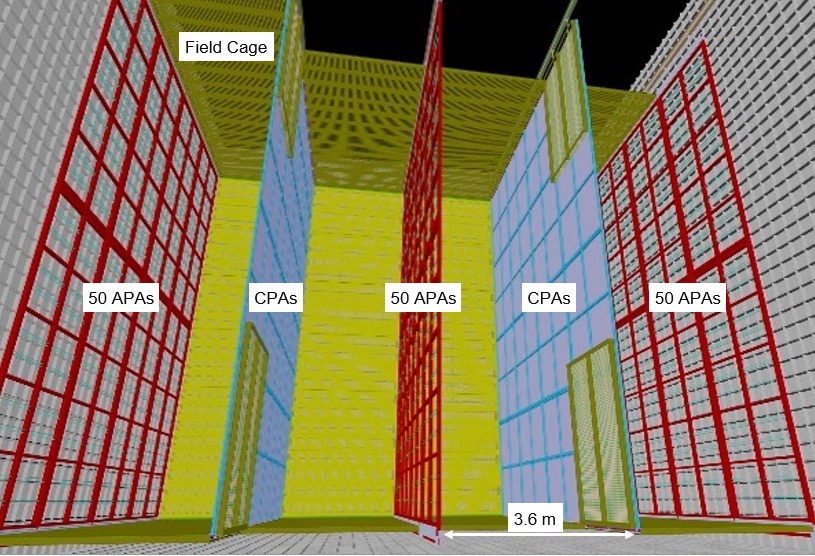
\includegraphics[width=0.7\textwidth]{DUNE_TPC.PNG}
\end{dunefigure}

%In MCC6.0, we simulated 3 types of beam neutrinos (unoscillated $\nu_\mu$'s, fully-oscillated $\nu_{e}$'s and fully-oscillated $\nu_\tau$'s), atmospheric neutrinos, supernova neutrinos, proton decays and cosmogenic events in the far detector. 
To save processing time, all the \dword{fd} samples except the cosmogenics sample were simulated using a smaller version of the full \nominalmodsize far \dword{detmodule} geometry. This geometry is \SI{13.9}{m} long, \SI{12}{m} high and \SI{13.3}{m} wide, which consists of 12 \dword{apa}s and 24 \dword{cpa}s. % anne fixed TPCs. 
%In the default configuration, the TPC wire spacing is 5 mm, the wire angle is 36$^{\circ}$ and the neutrino beam is parallel to the wire planes. 
Figure~\ref{fig:dune_apa} shows the detailed structure of an \dword{apa}. %We also generated special samples where the wire spacing is 3 mm or the wire angle is 45$^{\circ}$ or the neutrino beam is perpendicular to the wire planes for the detector optimization studies. 

\begin{figure}[!ht]
\centering
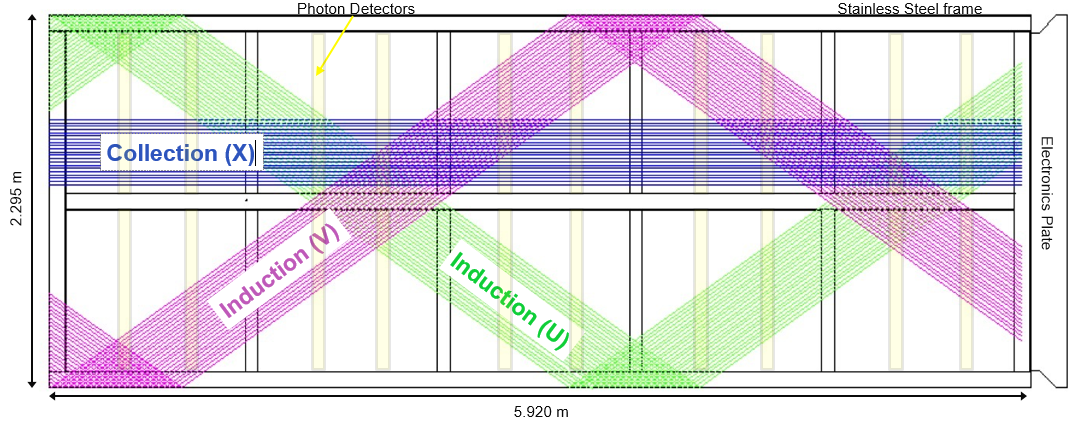
\includegraphics[width=0.7\textwidth]{DUNE_APA.PNG}
\caption{The detailed structure of the \dword{apa} is shown. Each \dword{apa} consists of four wrapped induction wire planes and two collection wire planes.
The \dword{pd} is sandwiched between the two collection wire planes.}
\label{fig:dune_apa}
\end{figure}

For the simulation chain, each sample is simulated in three steps: generation (gen), {\sc geant4} tracking (g4), TPC signal simulation, and digitization (detsim). The first step is unique for each sample while the second and the third steps are mostly identical for all samples. 

%%%%%%%%%%%%%%%%%%%%%%%%%%%%%%%
\subsection{Neutrino Flux Modeling}
\label{sec:tools-mc-flux}
%{\it Assigned to:} {\bf Laura Fields} with contributions from Zarko Pavlovic and Luke Pickering.

Neutrino fluxes were generated using G4LBNF, a \textsc{Geant}4\xspace-based simulation of the LBNF neutrino beam.  The simulation was configured to use a detailed description of the LBNF optimized beam design~\cite{optimizedbeamcdr}.  That design starts with a \SI{1.2}{MW}, \SI{120}{\GeV} primary proton beam that impinges on a \SI{2.2}{m} long, \SI{16}{mm} diameter cylindrical graphite target.  Hadrons produced in the target are focused by three magnetic horns operated with \SI{300}{kA} currents.  The target chase is followed by a \SI{194}{m} helium-filled decay pipe and a hadron absorber.  The focusing horns can be operated in forward or reverse current configurations, creating neutrino and antineutrino beams, respectively.   

\begin{dunefigure}[Visualization of the focusing system as simulated in g4lbnf]{fig:beam_vis}
{Visualization of the focusing system as simulated in g4lbnf.}
    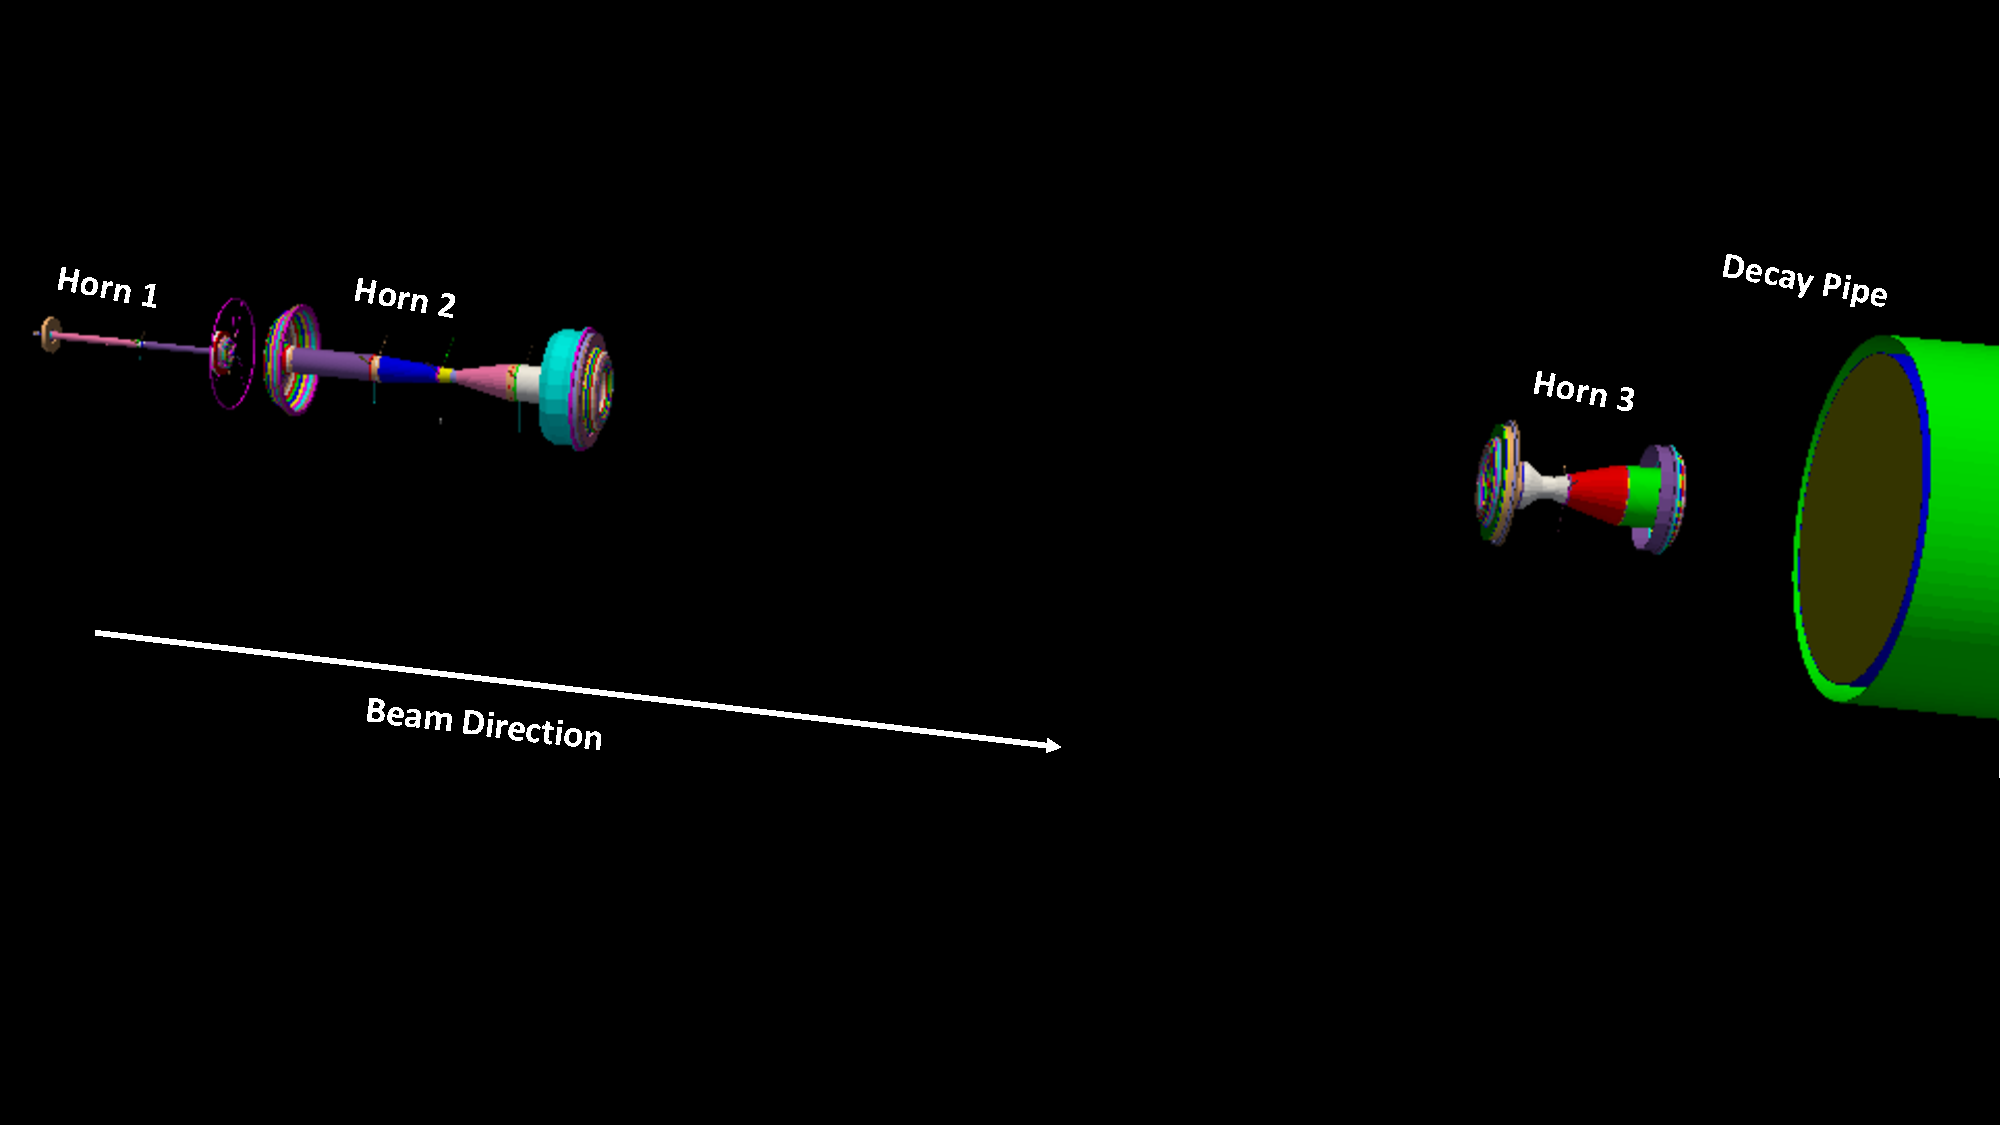
\includegraphics[width=0.7\textwidth]{Beamline_optimized_sept2017.pdf}\end{dunefigure}


The optimized LBNF neutrino beam design is the result of several years of effort by LBNF and DUNE to identify a focusing system optimized to DUNE's long-baseline physics goals.  This process began with a genetic algorithm that scanned simulations of many different horn and target geometries to identify those that produced the optimal sensitivity to \dword{cpv}.  The specific metric used was estimated sensitivity to 75\% of \dword{cp} phase space after \ktmwyr{300}  %kT MW years 
of exposure, taking into account the number and neutrino spectra of all neutrino flavors. The resulting beam effectively optimized flux at the first and second oscillation maxima, which also benefits measurements of other oscillation parameters.  The output of the genetic algorithm was a simple design including horn conductor and target shapes.  This design was transformed into a detailed conceptual design by LBNF engineers, and iterated with DUNE physicists to ensure that engineering changes had minimal impact on physics performance.  Relative to the previous NuMI-like design, the optimized design reduces the time to three-sigma coverage of 75\% of \dword{cp} phase space by 42\%, which is equivalent to increasing the mass of the far detector by 70\%.  It also substantially increases sensitivity to the mass hierarchy and improves projected resolution to quantities such as $\sin^22\theta_{13}$ and $\sin^2\theta_{23}$~\cite{fields_doc_2901}.        

\subsubsection{On-axis Neutrino Flux and Uncertainties}

%\fixme{in figure 4, near or far? the captions don't match. anne}
%ZP: It is near. Fixed the caption
\begin{dunefigure}[Neutrino fluxes at the near detector]{fig:flux_flavor}
{Predicted neutrino fluxes at the near detector for neutrino mode (left) and antineutrino mode (right). From top to bottom shown are muon neutrino, muon antineutrino, electron neutrino, and electron antineutrino fluxes.}
    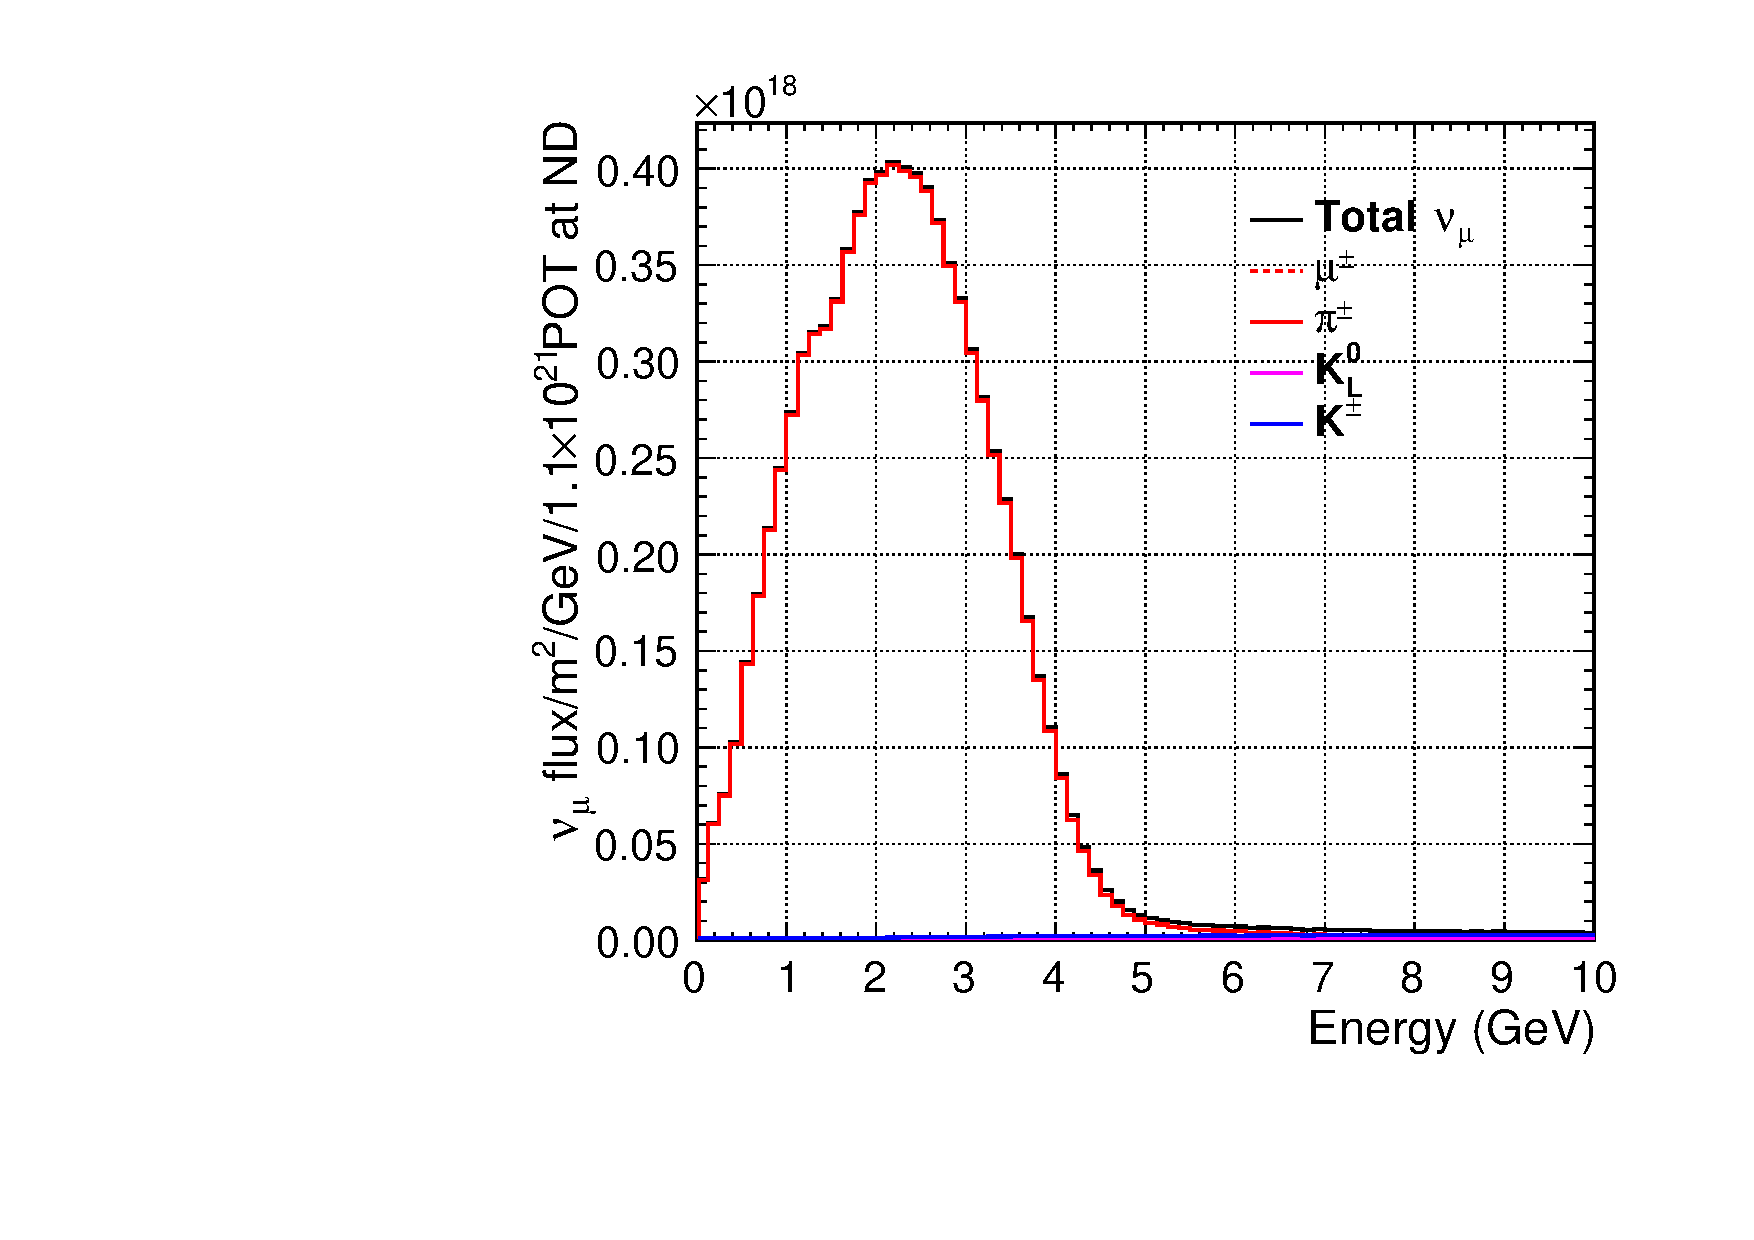
\includegraphics[width=0.35\textwidth]{graphics/dune_neutrino_nd_numu.pdf}
     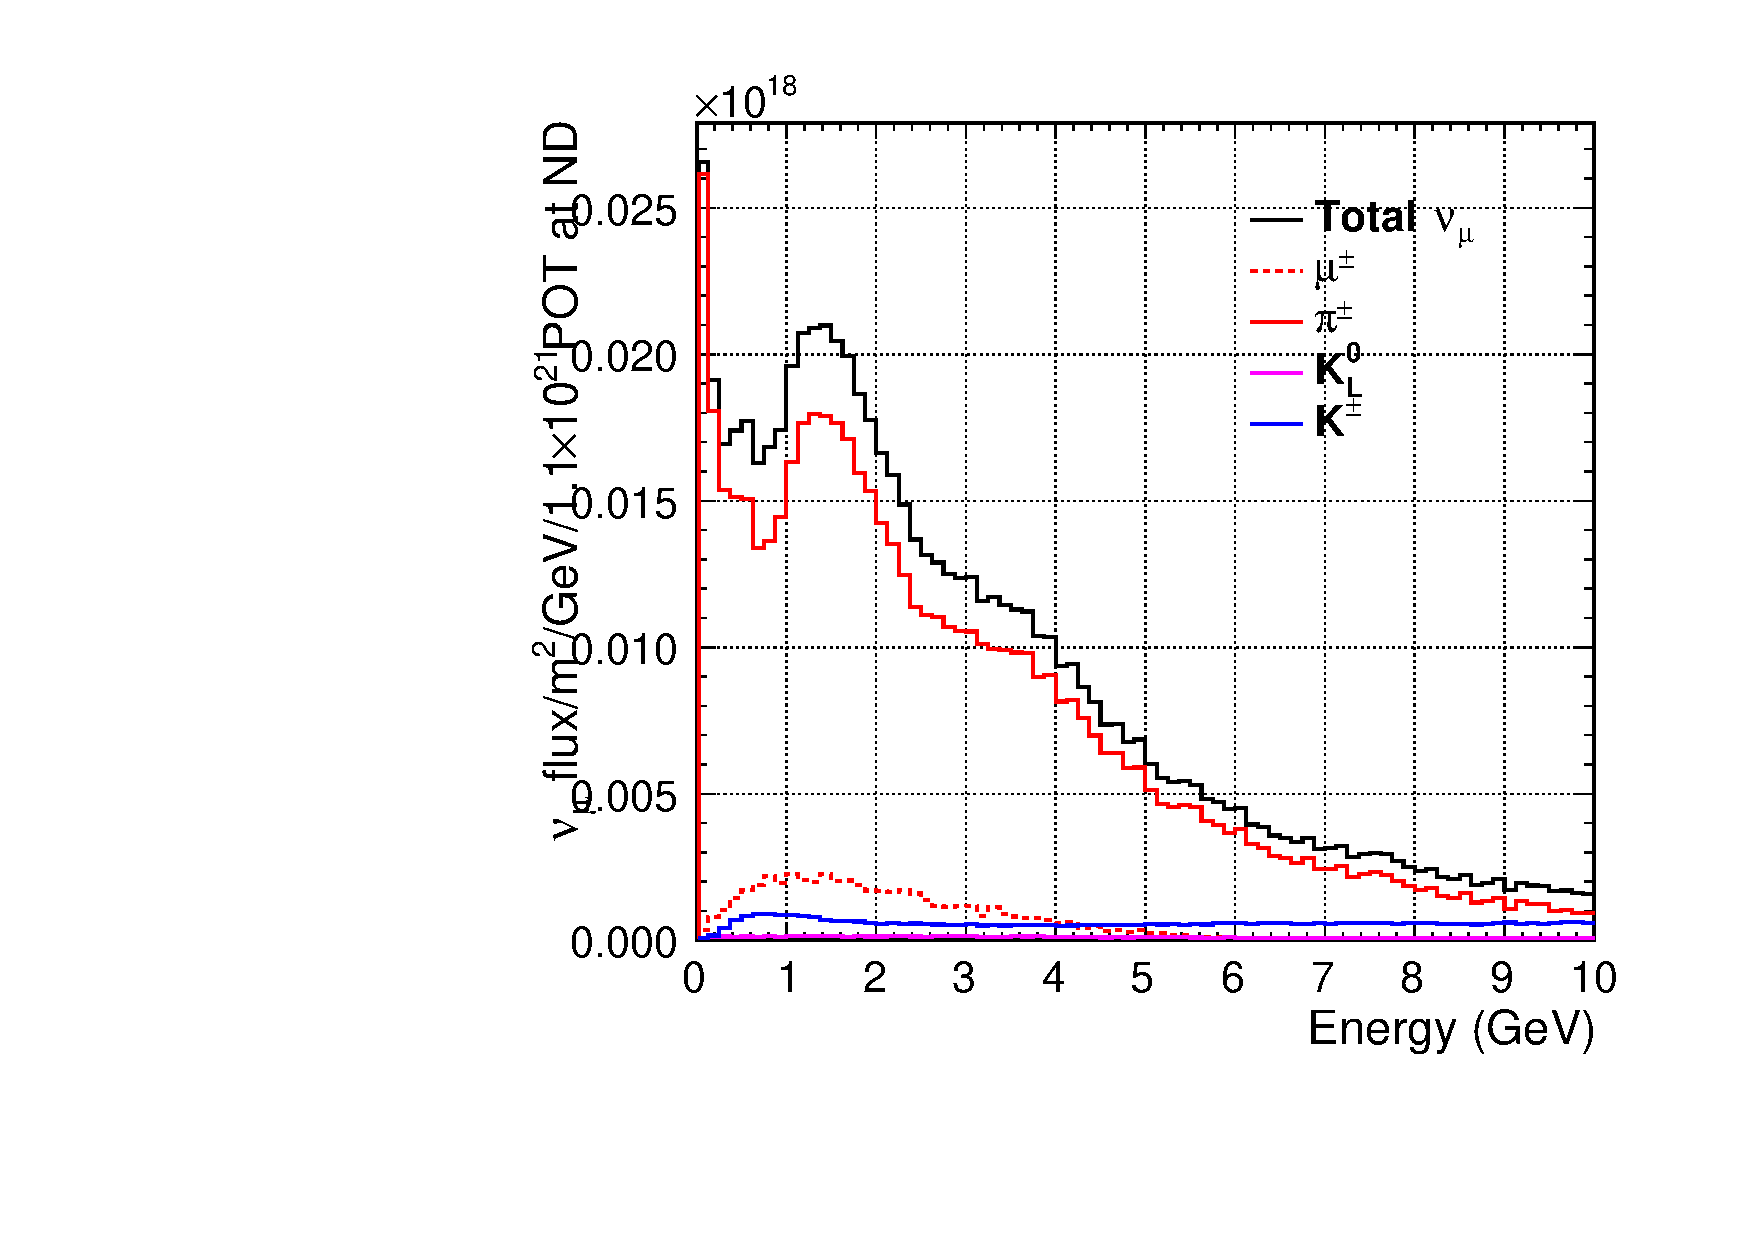
\includegraphics[width=0.35\textwidth]{graphics/dune_antineutrino_nd_numu.pdf}
    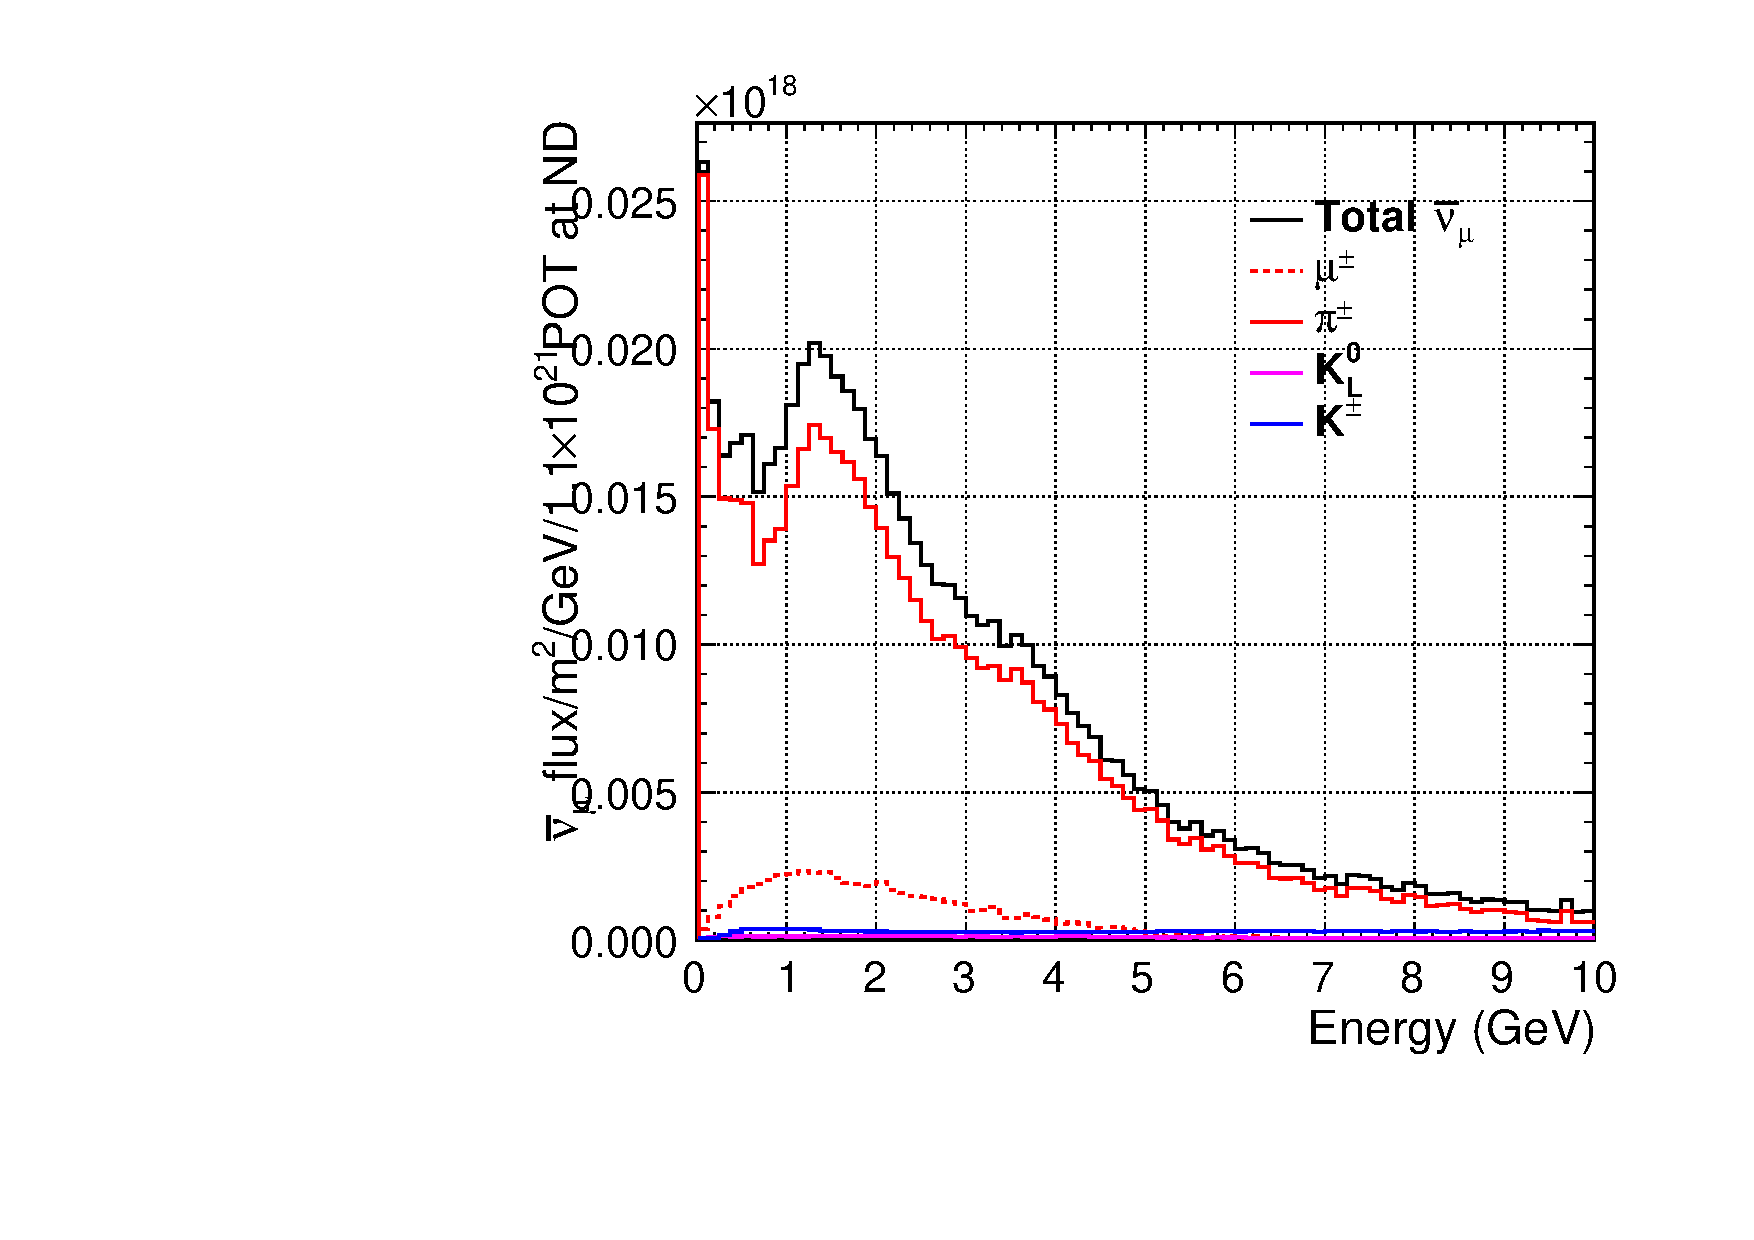
\includegraphics[width=0.35\textwidth]{graphics/dune_neutrino_nd_numubar.pdf}
     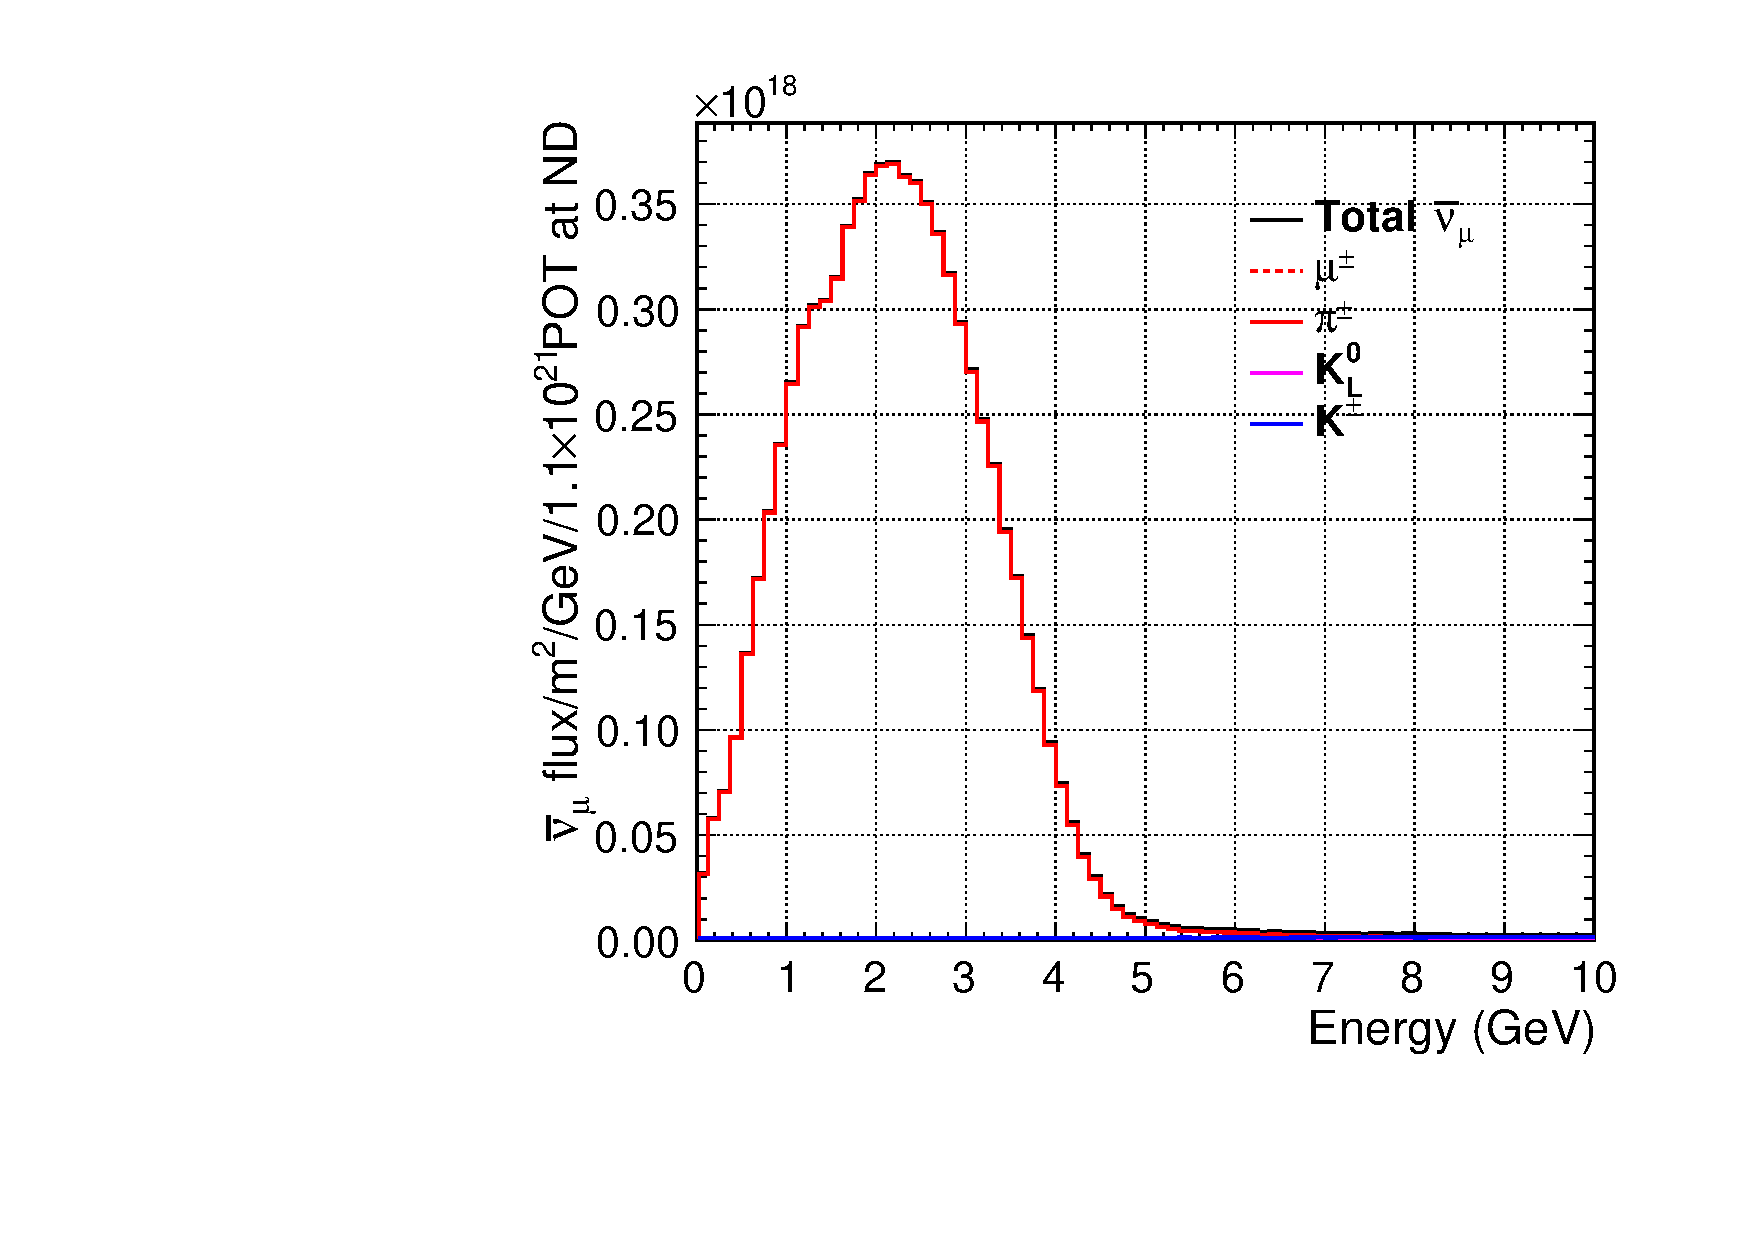
\includegraphics[width=0.35\textwidth]{graphics/dune_antineutrino_nd_numubar.pdf}
    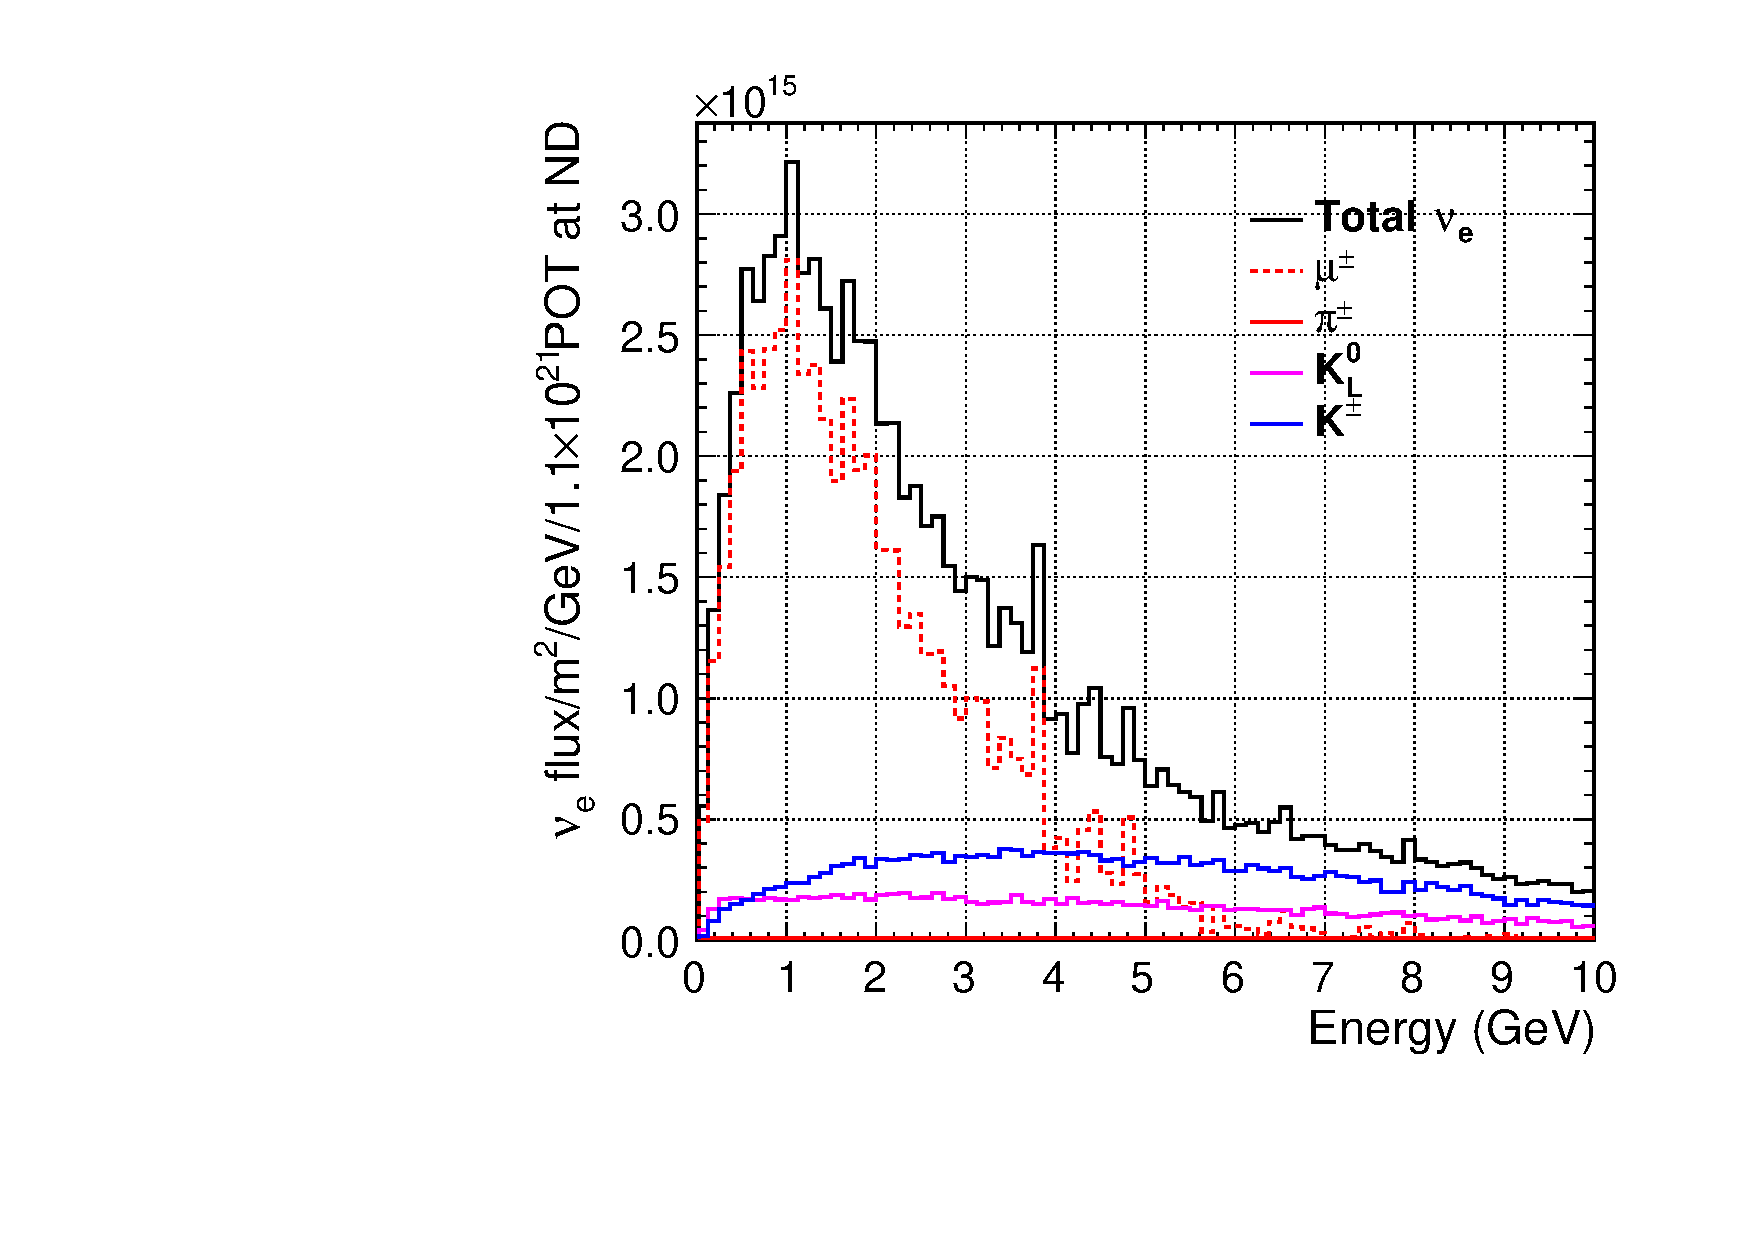
\includegraphics[width=0.35\textwidth]{graphics/dune_neutrino_nd_nue.pdf}
     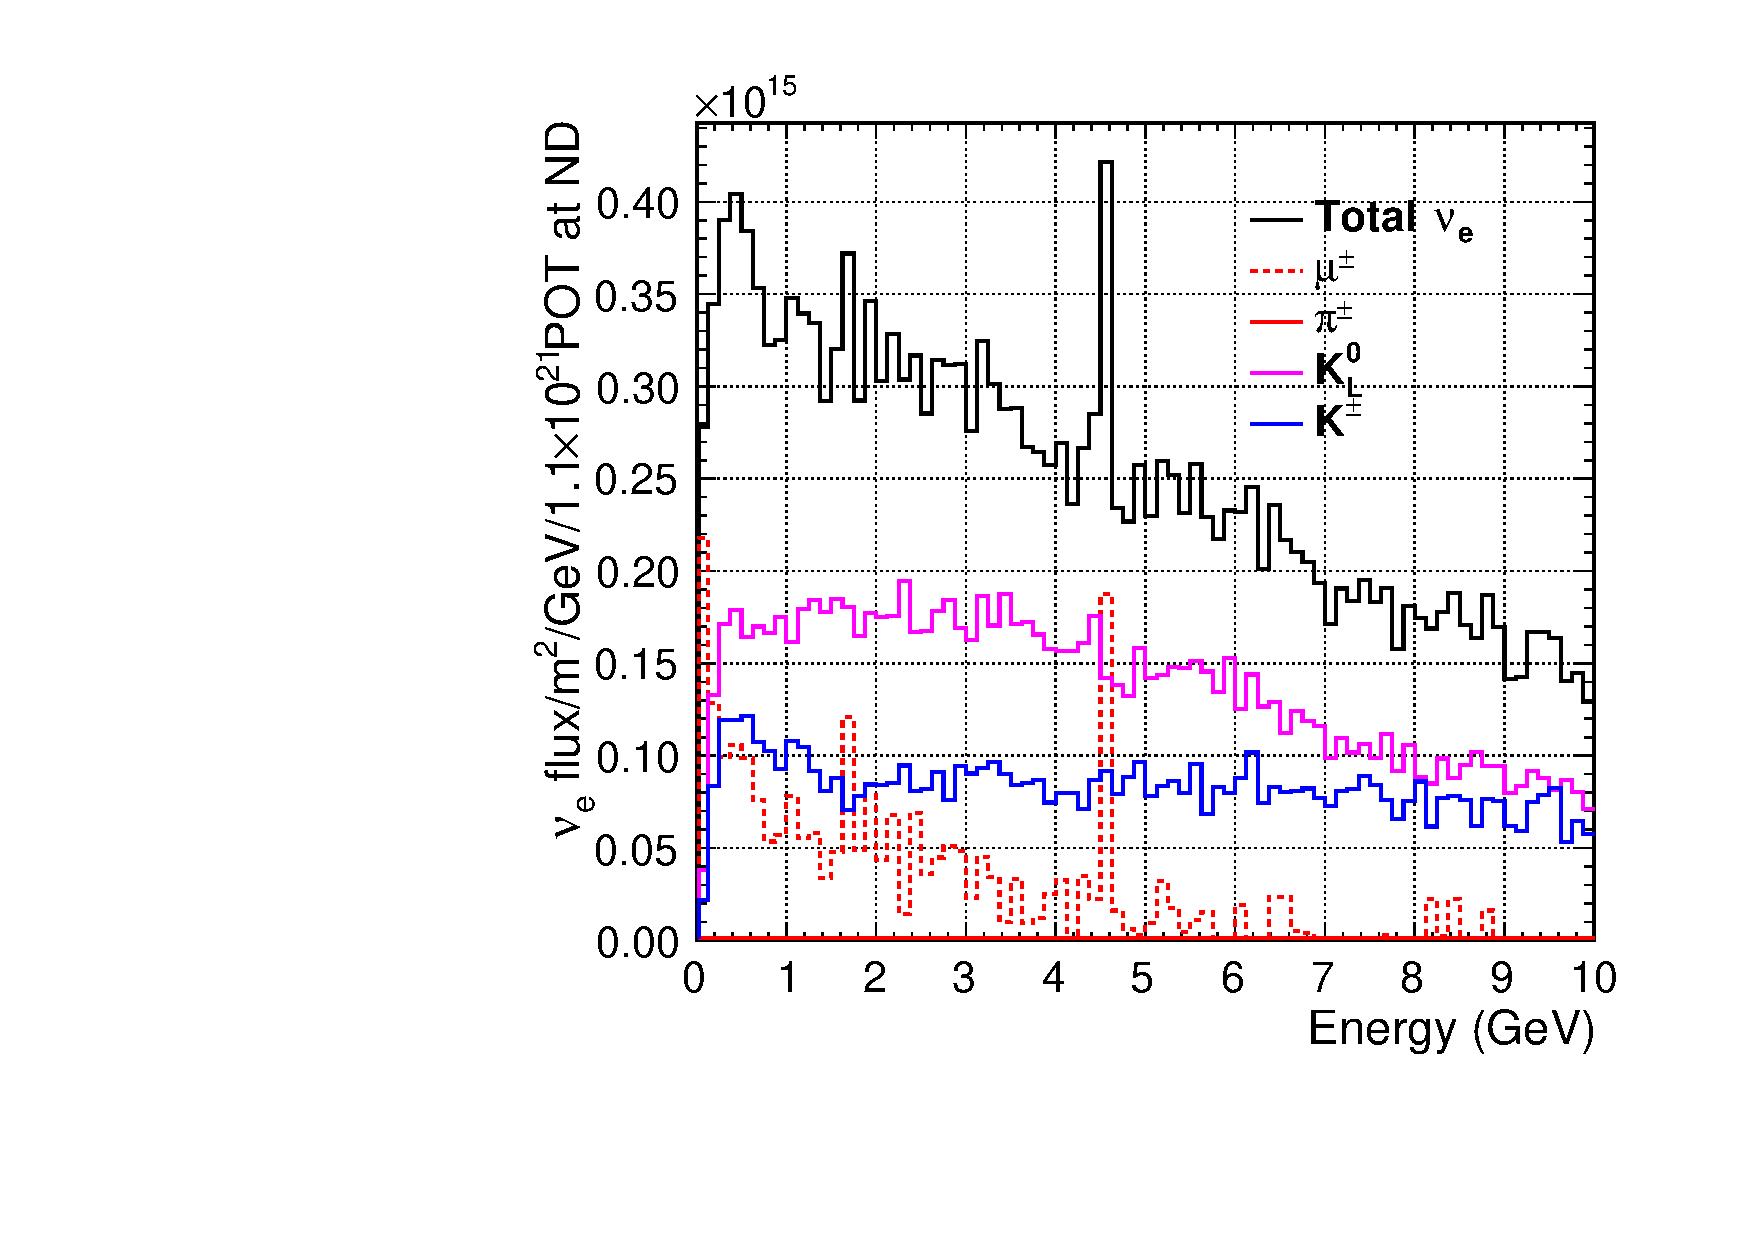
\includegraphics[width=0.35\textwidth]{graphics/dune_antineutrino_nd_nue.pdf}
    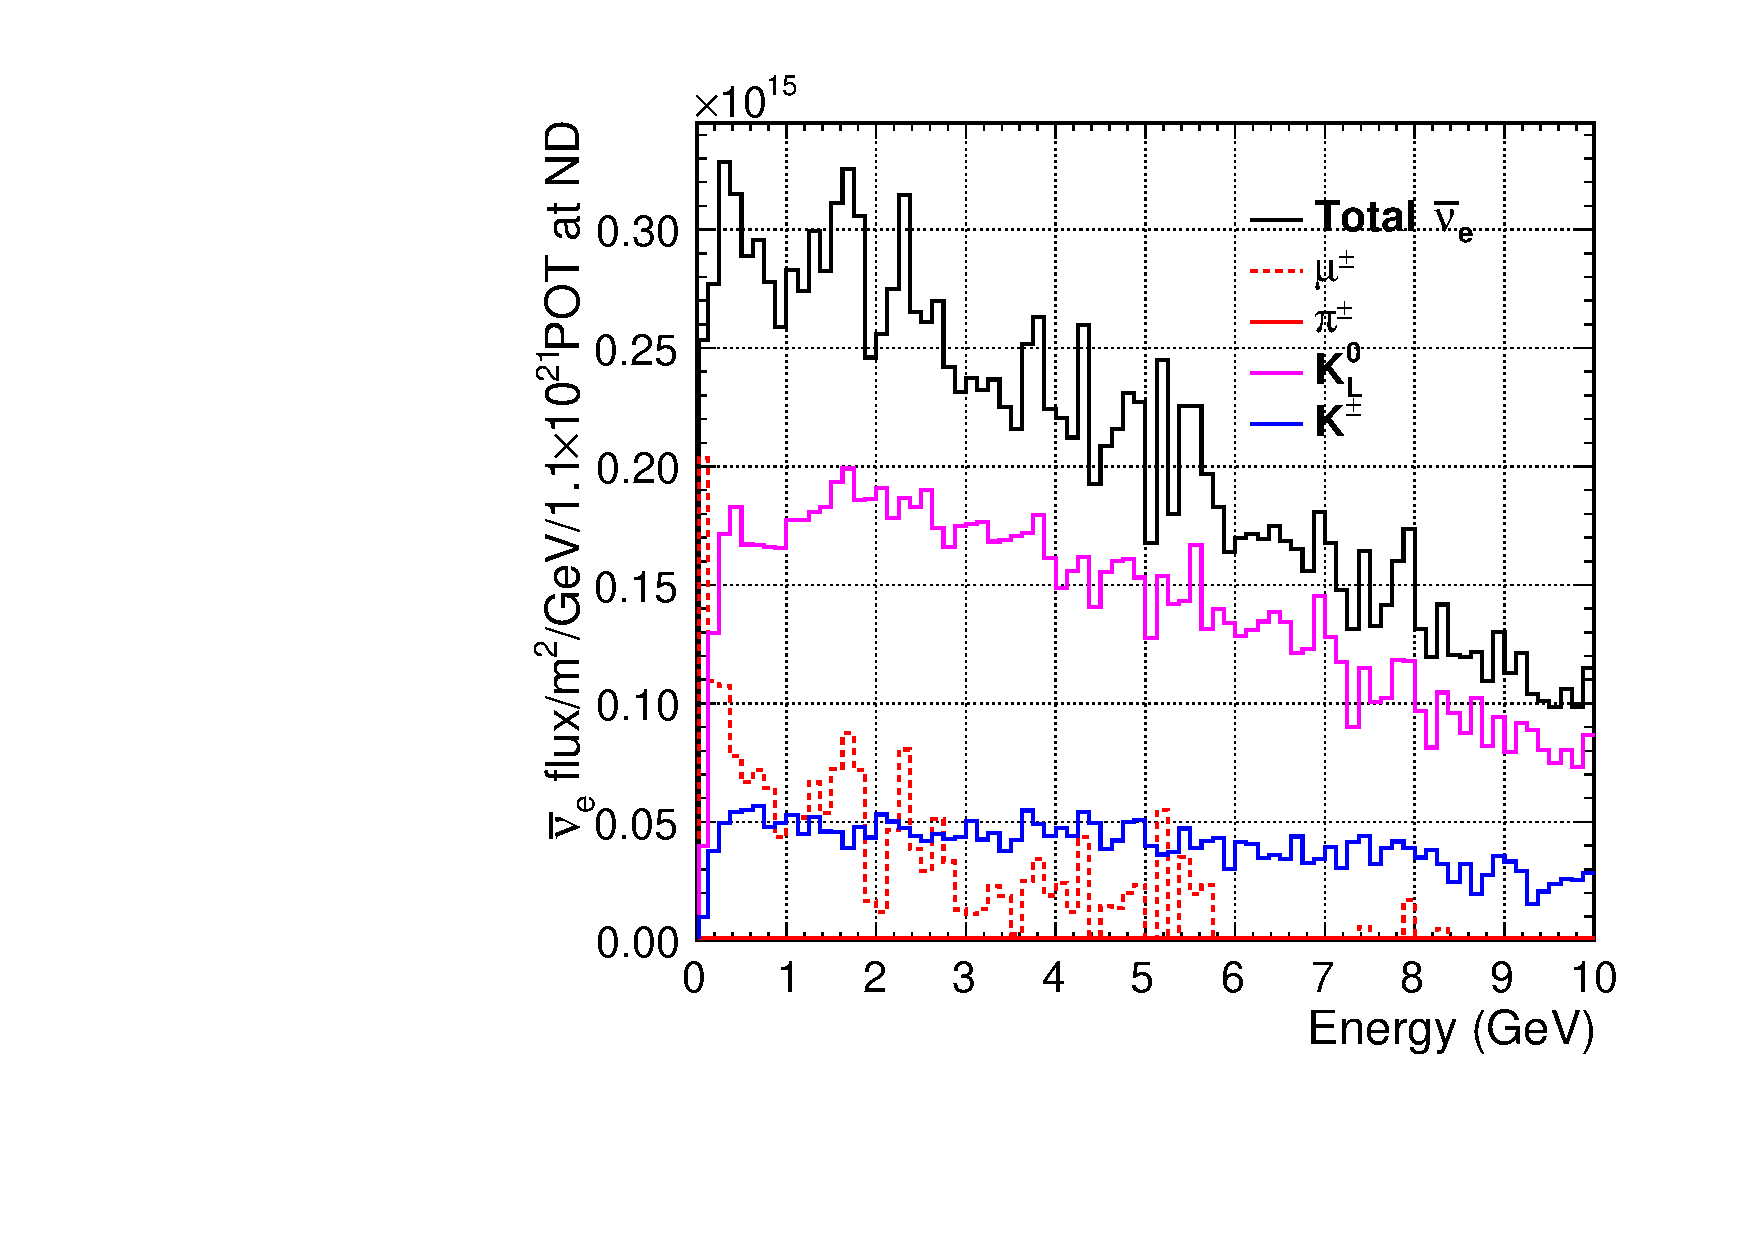
\includegraphics[width=0.35\textwidth]{graphics/dune_neutrino_nd_nuebar.pdf}
     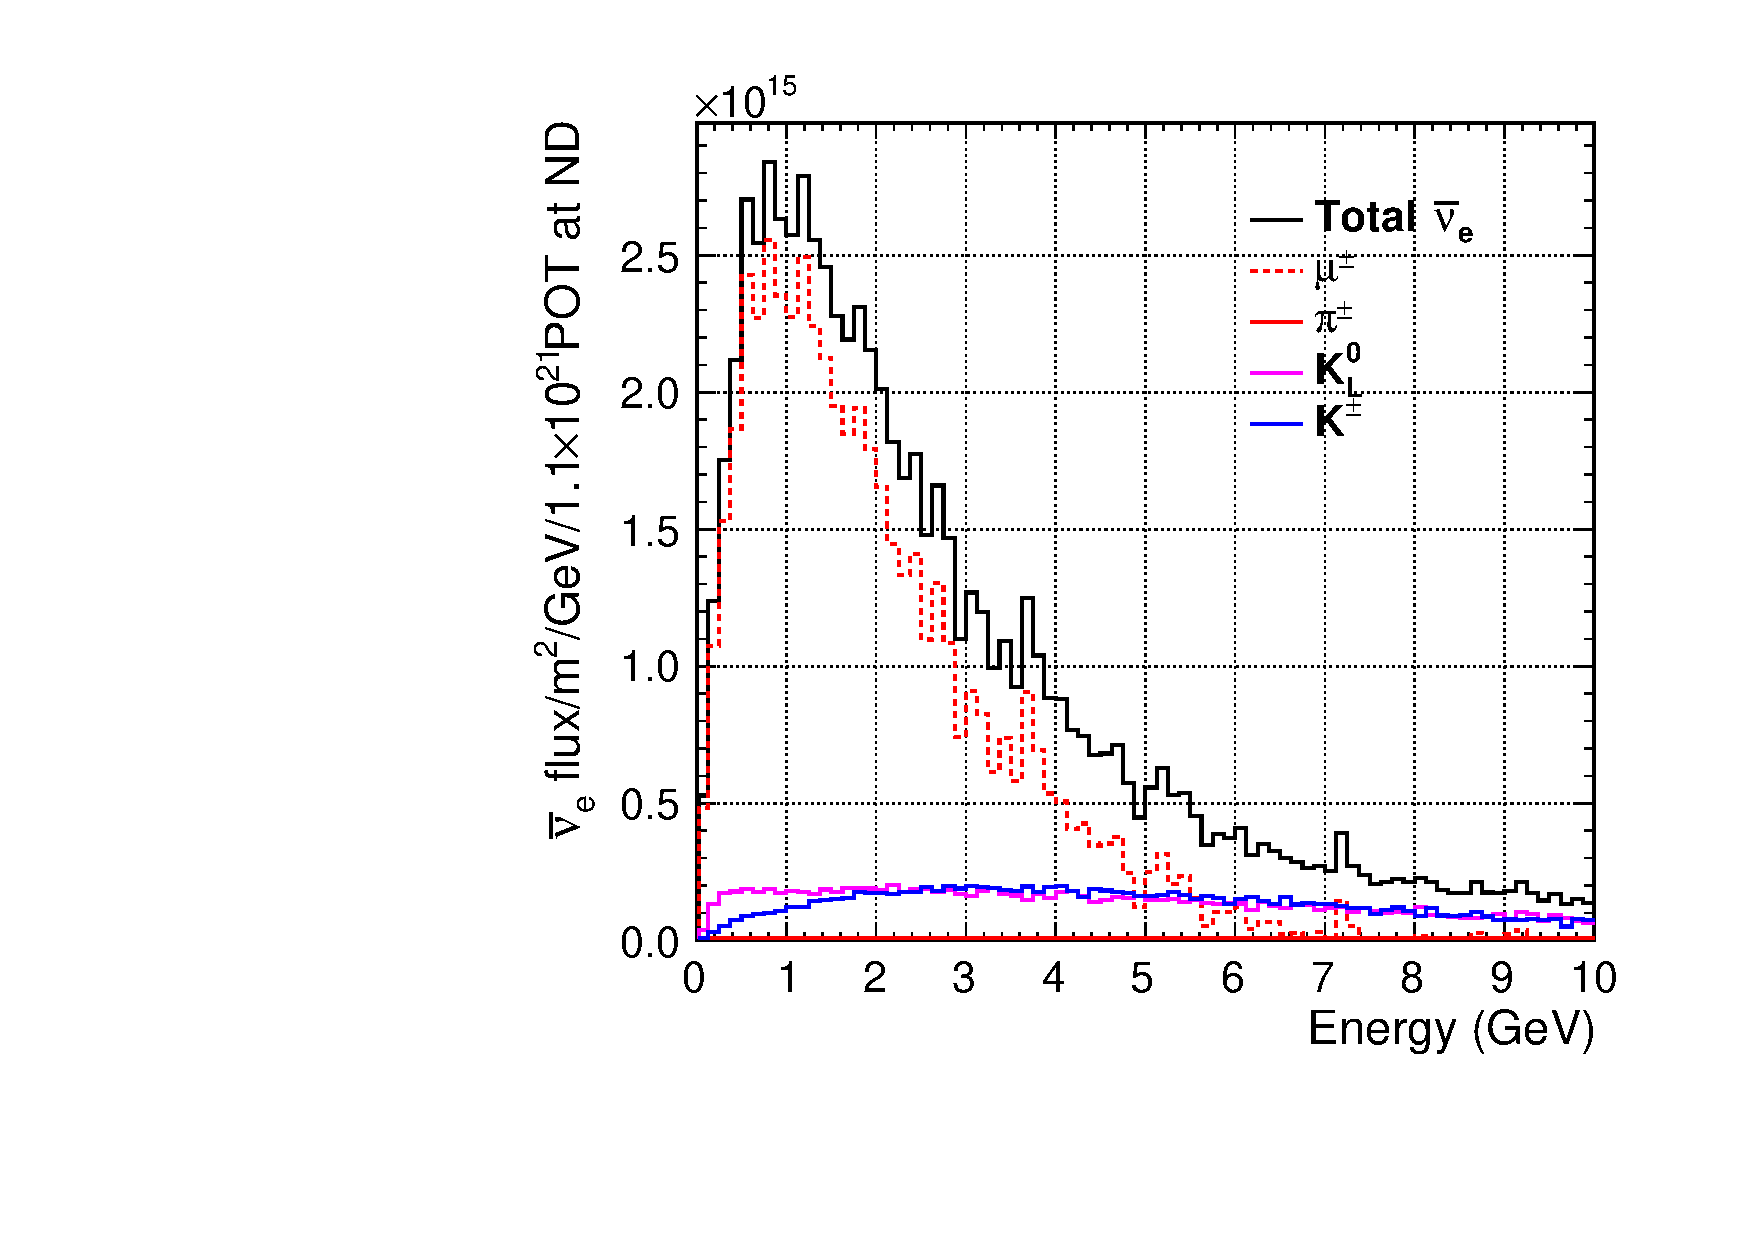
\includegraphics[width=0.35\textwidth]{graphics/dune_antineutrino_nd_nuebar.pdf}
\end{dunefigure}

%\todo{Add numbers for flavor composition of beam}
%zp: added fractions for optimized beam at FD
%zp: updated fig:flux_flavor to Optimized 
The predicted neutrino fluxes for neutrino and antineutrino mode configurations of LBNF are shown in Figure~\ref{fig:flux_flavor}.  In neutrino (antineutrino) mode, the beams are 92\% (90.4\%) muon neutrinos (antineutrinos), with wrong-sign contamination making up 7\% (8.6\%) and electron neutrino and antineutrino backgrounds 1\% (1\%).  Although %there is also expected to be 
we expect a small non-zero intrinsic tau neutrino flux, this is not simulated by G4LBNF.  Nor are neutrinos arising from hadron decay at rest. % are also not simulated.  

\begin{dunefigure}[Flux uncertainties at the \dword{fd} as a function of neutrino energy]{fig:flux_uncertainties_flavor}
{Flux uncertainties at the far detector as a function of neutrino energy in neutrino mode (left) and antineutrino mode (right) for, from top to bottom, muon neutrinos, muon antineutrinos, electron neutrinos and electron antineutrinos. (To be updated.)   }
    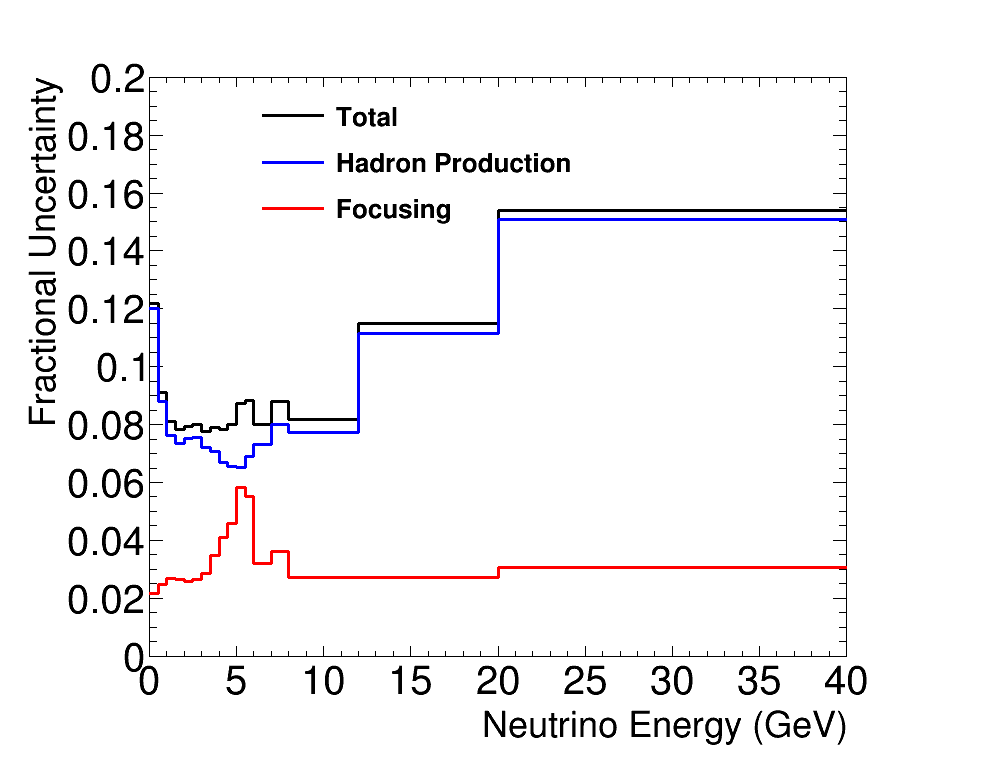
\includegraphics[width=0.4\textwidth]{error_overlay_numu_neutrino_FD_opt.png}
    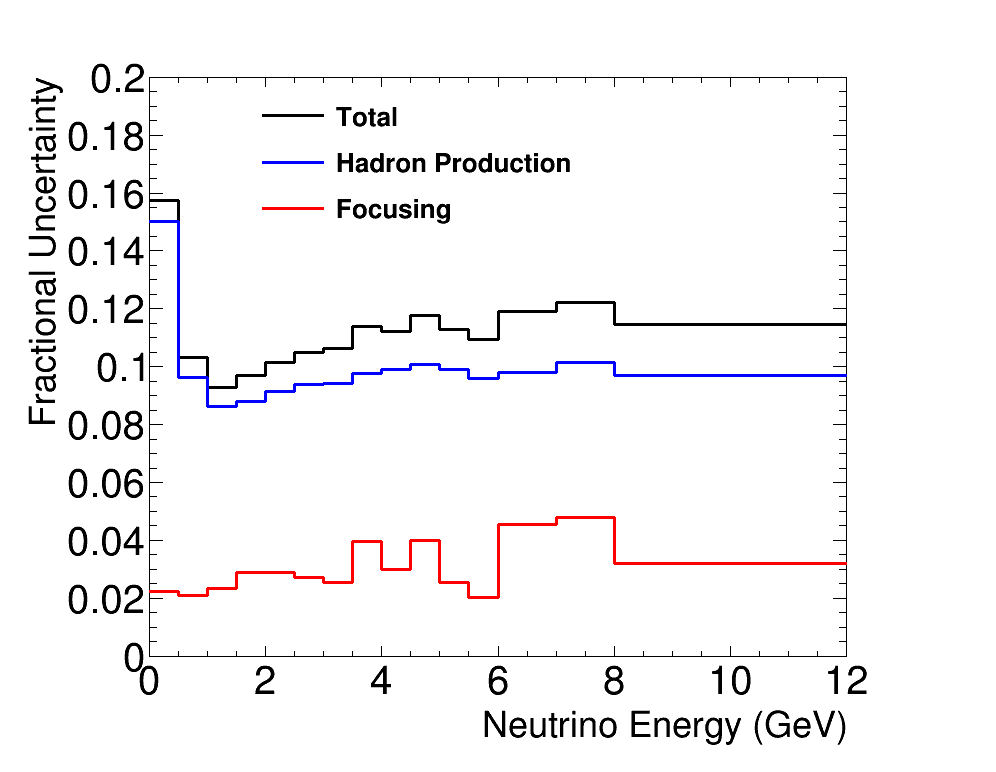
\includegraphics[width=0.4\textwidth]{error_overlay_numu_antineutrino_FD_opt.png}
    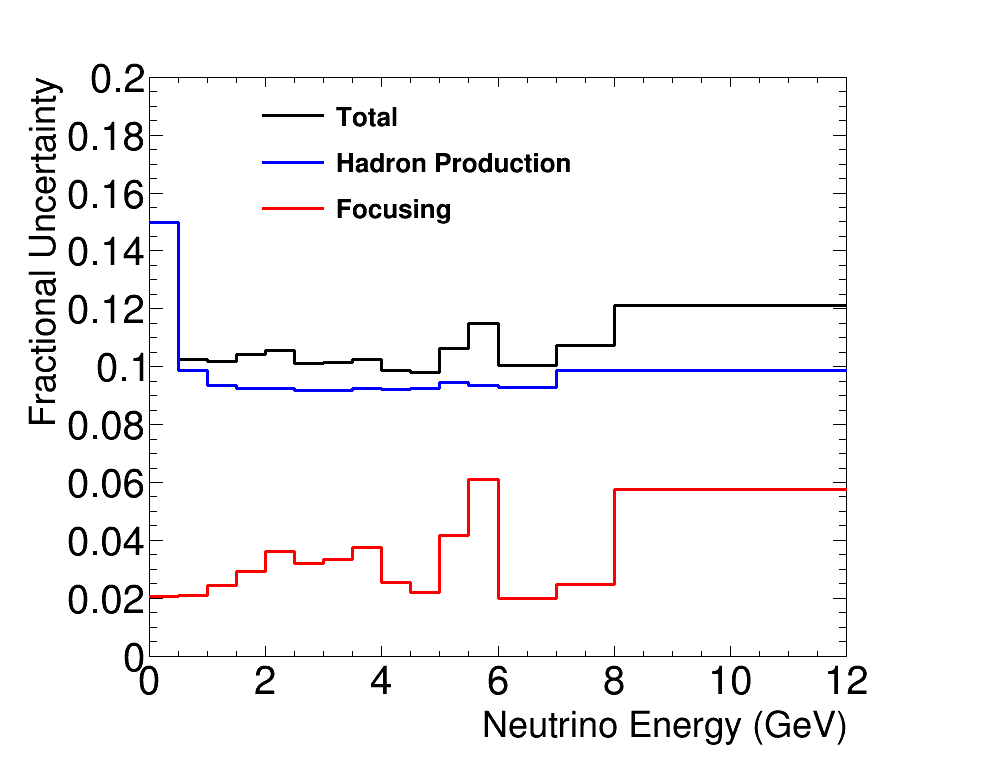
\includegraphics[width=0.4\textwidth]{error_overlay_numubar_neutrino_FD_opt.png}
    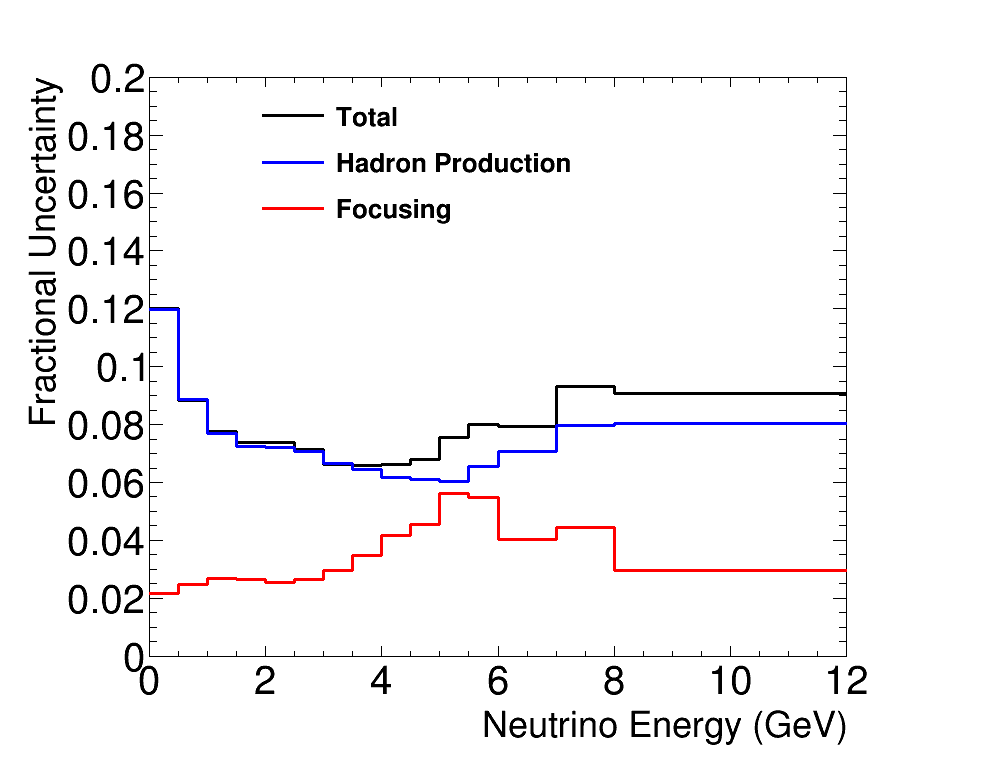
\includegraphics[width=0.4\textwidth]{error_overlay_numubar_antineutrino_FD_opt.png}
        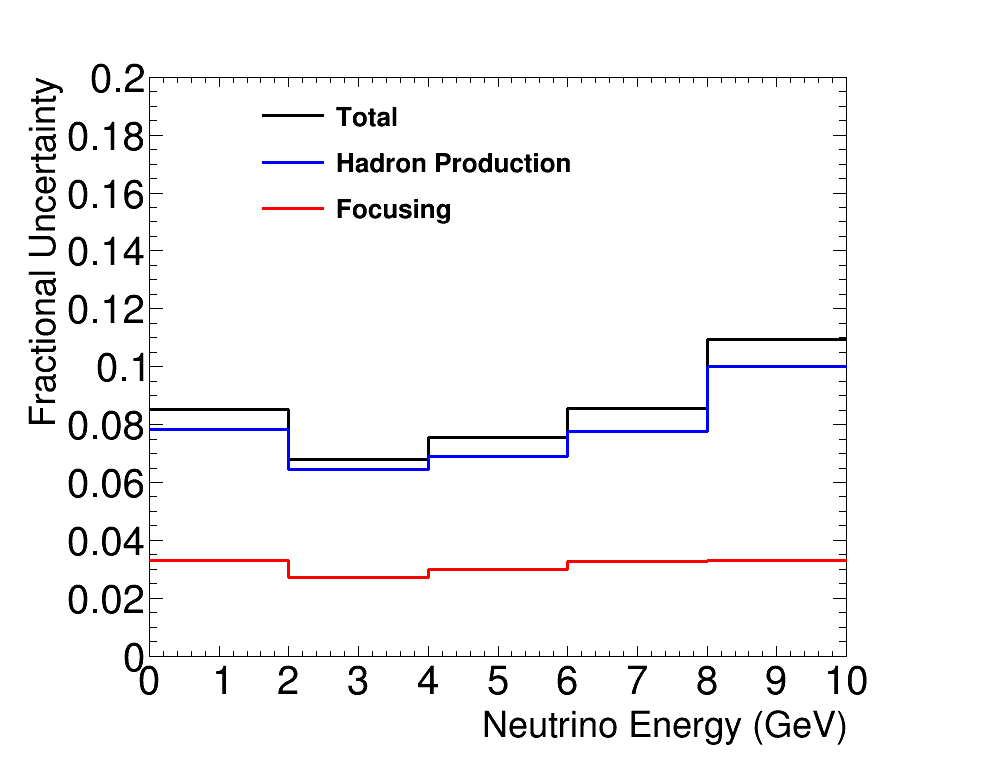
\includegraphics[width=0.4\textwidth]{error_overlay_nue_neutrino_FD_opt.png}
    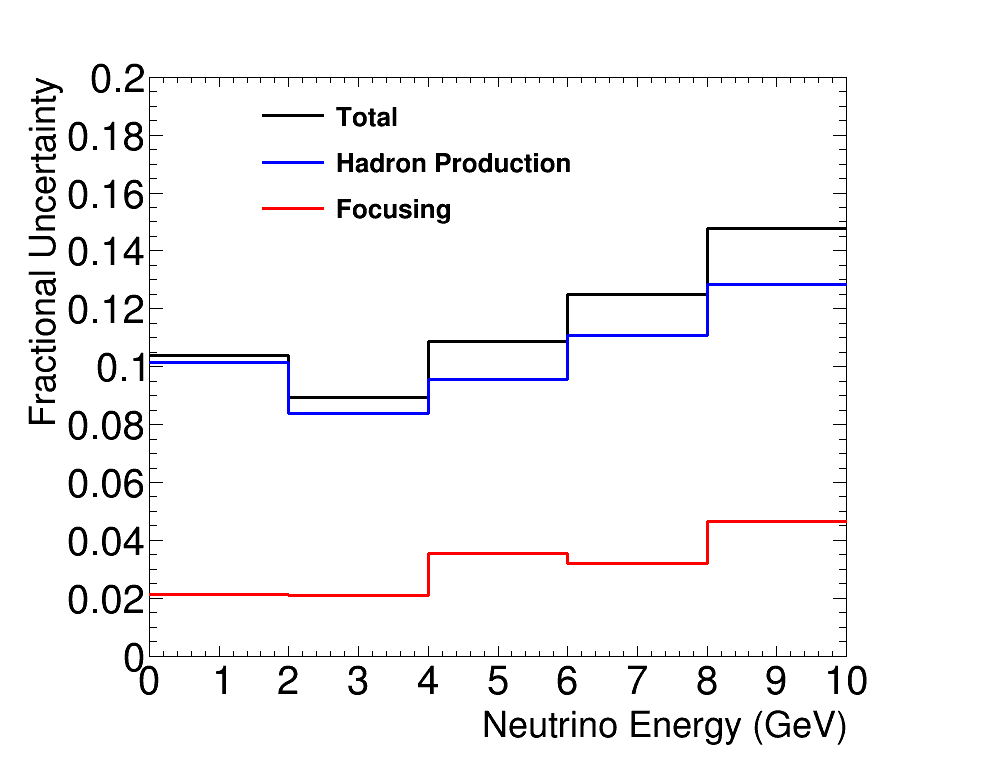
\includegraphics[width=0.4\textwidth]{error_overlay_nue_antineutrino_FD_opt.png}
        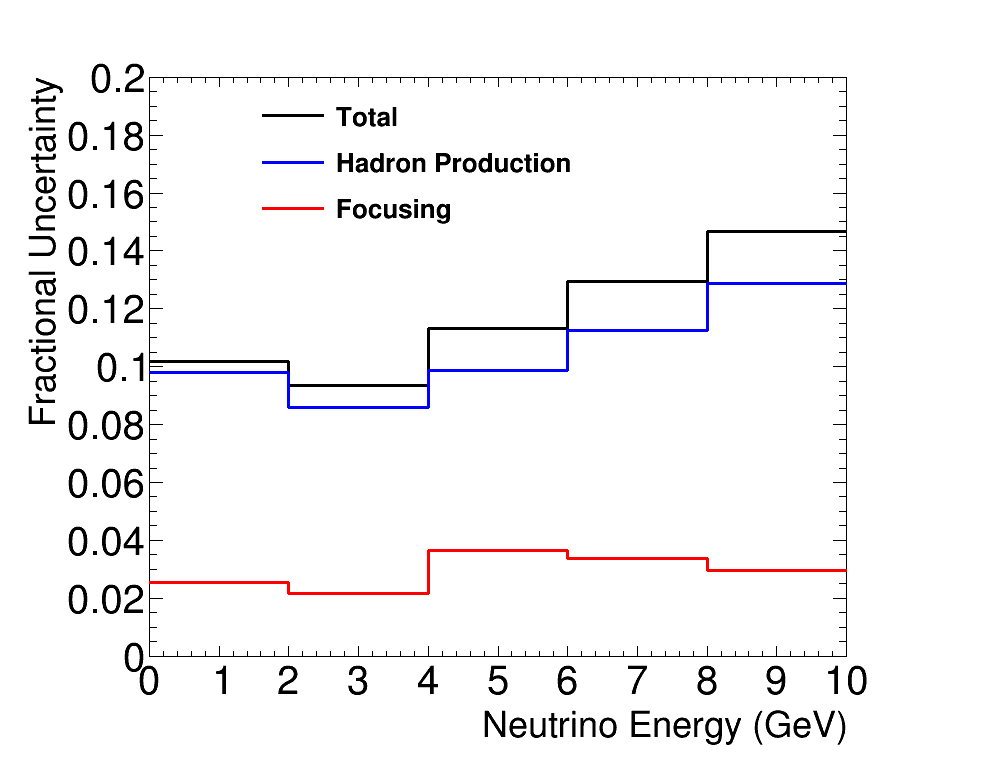
\includegraphics[width=0.4\textwidth]{error_overlay_nuebar_neutrino_FD_opt.png}
    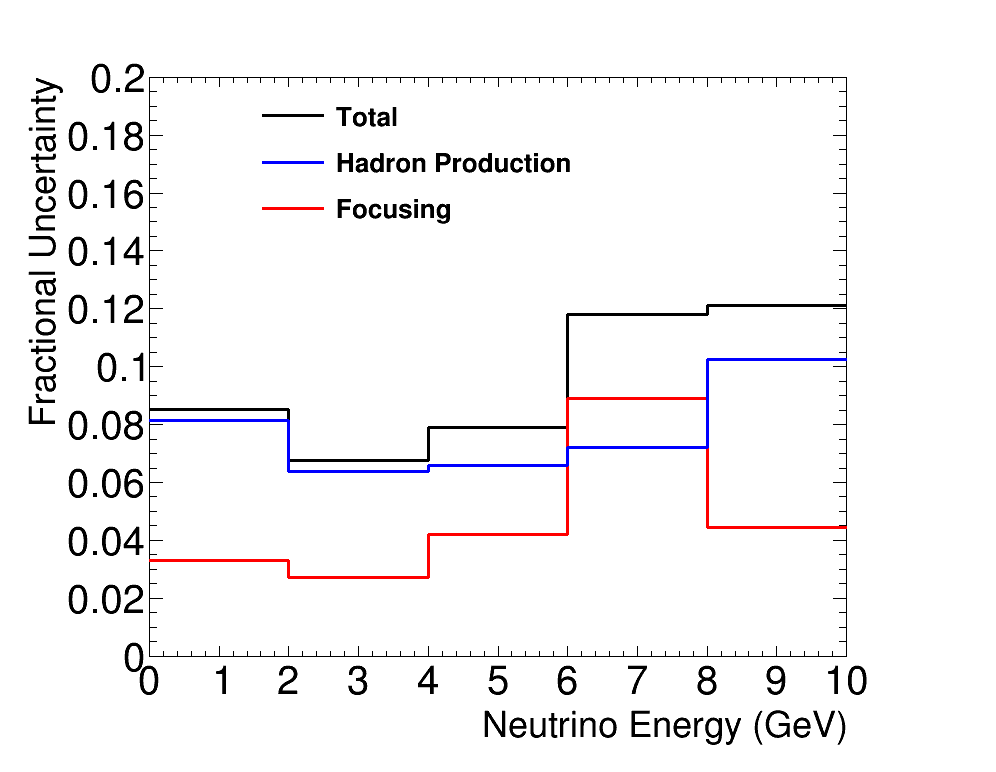
\includegraphics[width=0.4\textwidth]{error_overlay_nuebar_antineutrino_FD_opt.png}
    \end{dunefigure}

%\fixme{defin NDTF, PPFX. anne}
%ZP: expanded PPFX to Package to Predict the FluX (PPFX) and citation is also given for the package
%ZP: Removed NDTF since it will not be mentioned in final caption, just left comment that plots still need to be updated

\begin{dunefigure}[Focusing and hadron production uncertainties on the $\nu$ mode $\nu_{\mu}$ flux]{fig:flux_uncertainty_breakdown}
{Focusing (left) and hadron production (right) uncertainties on the neutrino mode muon neutrino flux at the \dword{fd}.  This is for an older beam design and will be updated to the latest.  }
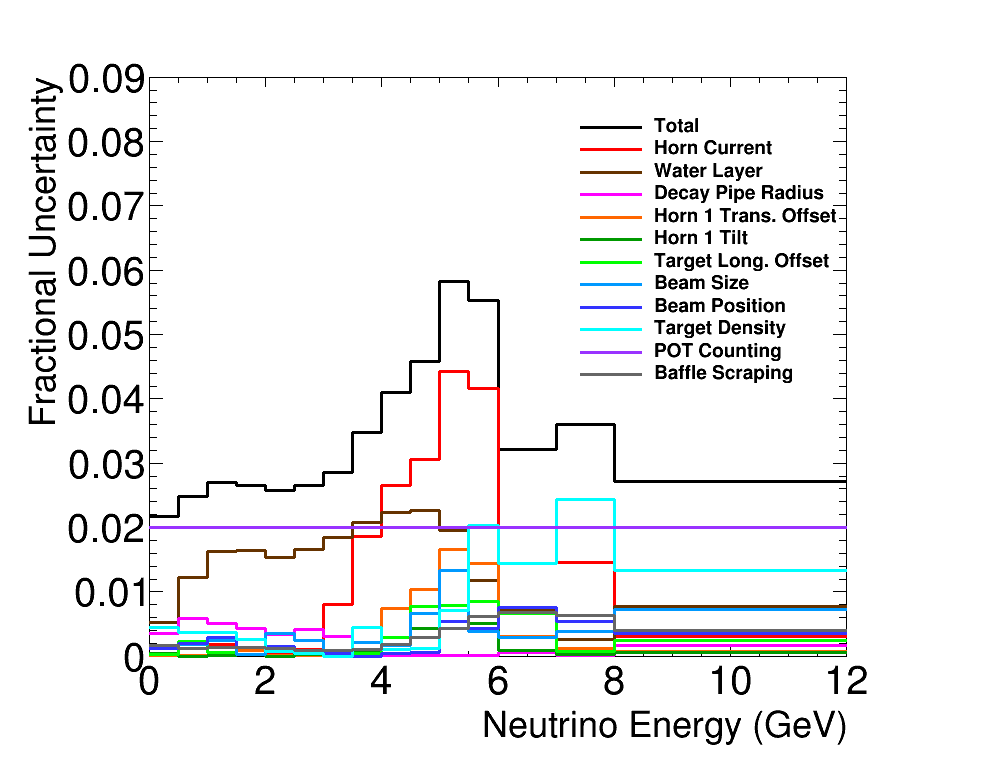
\includegraphics[width=0.45\textwidth]{focusing_error_overlay_numu_neutrino_FD_opt.png}
    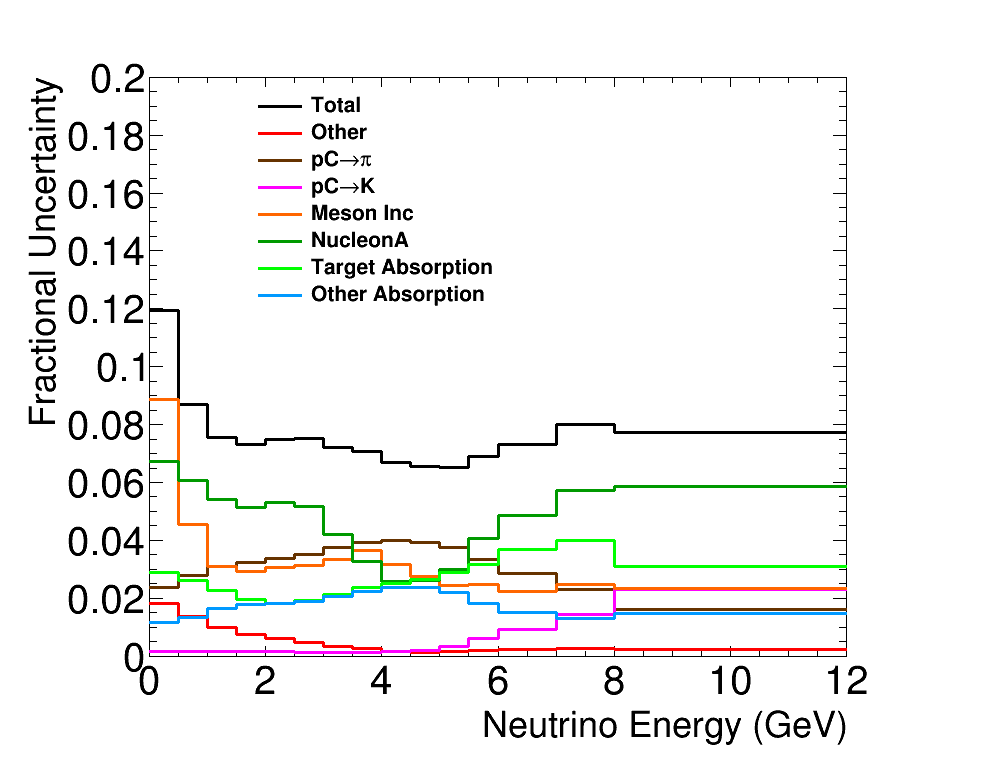
\includegraphics[width=0.45\textwidth]{HP_error_overlay_numu_neutrino_FD_opt.png}\end{dunefigure}

Uncertainties on the neutrino fluxes arise primarily from uncertainties in hadrons produced off the target and uncertainties in parameters of the beam such as horn currents and horn and target positioning (commonly called ``focusing uncertainties'').  Uncertainties on the neutrino fluxes arising from both of these categories of sources are shown in Figure~\ref{fig:flux_uncertainties_flavor}.  Hadron production uncertainties are estimated using the Package to Predict the FluX (PPFX) framework developed by the \minerva collaboration~\cite{Aliaga:2016oaz, AliagaSoplin:2016shs}, which assigns uncertainties for each hadronic interaction leading to a neutrino in the beam simulation, with uncertainties taken from thin target data (from e.g., the NA49~\cite{NA49} experiment) where available, and large uncertainties assigned to interactions not covered by data.  Focusing uncertainties are assessed by altering beamline parameters in the simulation within their tolerances and observing the resulting change in predicted flux.  A breakdown of the hadron production and focusing uncertainties into various components are shown in Figure~\ref{fig:flux_uncertainty_breakdown} for the neutrino mode muon neutrino flux at the \dword{fd}.    

At most energies, hadron production uncertainties are dominated by the ``NucleonA'' category, which includes proton and neutron interactions that are not covered by external data.  At low energies, uncertainties due to pion reinteractions (denoted ``Meson Inc'') dominate.   The largest source of focusing uncertainty arises from a 1\% uncertainty in the horn current, followed by a 2\% flat uncertainty in the number of protons impinging on the target.   For all neutrino flavors and all neutrino energies, hadron production uncertainties are larger than focusing uncertainties.  However, hadron production uncertainties are expected to decrease in the next decade, as more thin target data becomes available.  Hadron production measurements taken with a replica target are also being considered and would substantially reduce the uncertainties.  

\begin{dunefigure}[Correlation of flux uncertainties]{fig:flux_uncertainty_correlation}
{Correlation of flux uncertainties.  Each block of neutrino flavor corresponds to bins of energy with bin boundaries of [0.0, 0.5, 1.0, 1.5, 2.0, 2.5, 3.0, 3.5, 4.0, 4.5, 5.0, 5.5, 6.0, 8.0, 10.0, 15.0, 20.0, 40.0, 100.0] for muon neutrinos and antineutrinos and of [0.0, 2.0, 4.0, 6.0, 8.0, 10.0, 20.0, 100.0] for electron neutrinos and antineutrinos. }
    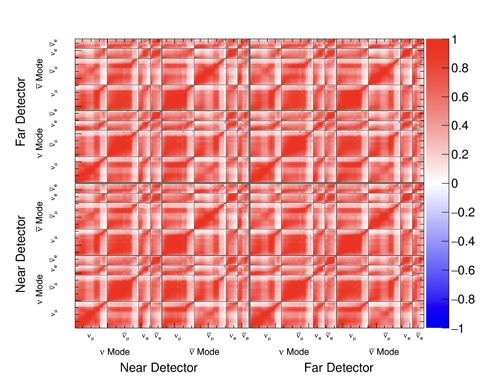
\includegraphics[width=0.9\textwidth]{correlation_ndtf_opt.png}\end{dunefigure}

Figure~\ref{fig:flux_uncertainty_correlation} shows correlations of the total flux uncertainties.  In general, the uncertainties are highly correlated across energy bins. However, the flux in the very high energy, coming predominantly from kaons, tends to be uncorrelated with flux at the peak, %dominated 
arising predominantly from pion decays.  Flux uncertainties are also highly correlated between the near and far detectors and between neutrino-mode and antineutrino-mode running.  The focusing uncertainties do not affect wrong-sign backgrounds, which reduces correlations between e.g., muon neutrinos and muon antineutrinos in the same running configuration in the energy bins where focusing uncertainties are significant.    

%Although the fluxes at the \dword{nd} and \dword{fd} are similar, they are not identical.  
The fluxes at the \dword{nd} and \dword{fd} are similar but not identical. Figure~\ref{fig:flux_nearfar} shows the ratio of the near and far neutrino-mode muon neutrino fluxes %at the near and far detectors 
and the uncertainties on the ratio.  The uncertainties are approximately 1\% or smaller except at the falling edge of the focusing peak, where they rise to 2\%, but are still much smaller than the uncertainty on the absolute fluxes.    And unlike the case for absolute fluxes, the uncertainty on the near-to-far flux ratio is dominated by focusing rather than hadron production uncertainties.  This ratio and its uncertainty are for the fluxes at the center of the near and far detectors,
%\fixme{which, near or far?}
%ZP: inserted "near and far" since it is for both thought this is not so relevant for far.
and do not take into account small variations in flux across the face of the \dword{nd}.     

\begin{dunefigure}[Ratio of neutrino-mode muon neutrino fluxes at the near and far detectors]{fig:flux_nearfar}
{Ratio of neutrino-mode muon neutrino fluxes at the near and far detectors (left) and uncertainties on the ratio (right).  To be updated. }
    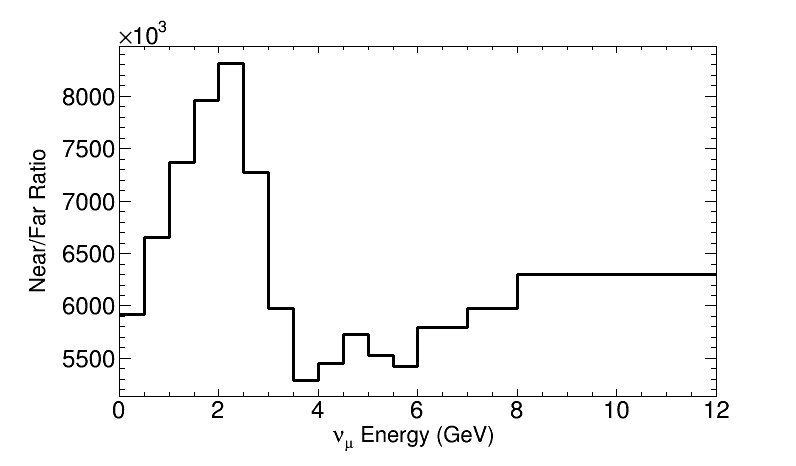
\includegraphics[width=0.45\textwidth]{nearfar.png}
     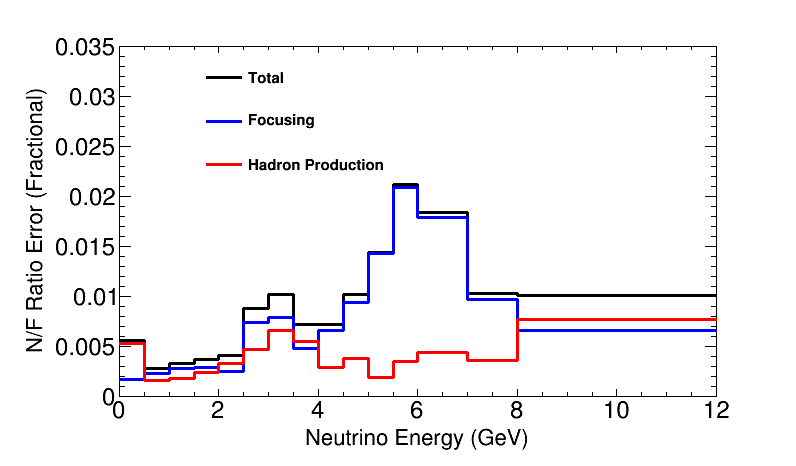
\includegraphics[width=0.45\textwidth]{nearfarunc.png}
\end{dunefigure}
\fixme{see the 'to be updated in figure}

\subsubsection{Off-axis Neutrino Flux and Uncertainties}

The neutrino flux spreads beyond the beam aimed directly at the \dword{fd}, and viable neutrino fluxes extend outward at the \dword{nd} hall.  For an ``off-axis'' angle relative to the initial beam direction, the subsequent neutrino energy spectrum is narrower and peaked at a lower energy than the on-axis spectrum. At \SI{575}{m}, the location of the \dword{nd} hall, a lateral shift of \SI{1}{m} corresponds to approximately a \ang{0.1} change in off-axis angle.  Furthermore, the DUNE-PRISM concept, in which the near detector \lartpc %is movable 
can be moved to enable  off-axis measurements, relies on this feature to help constrain systematic errors for the \dword{lbl} oscillation program as described in Section~\ref{sec:ch-nu-osc-06-ndconcept-offaxis}. A discussion of off-axis flux modeling is given in %the Appendix, in 
Section~\ref{sec:tools-app-flx-offaxis}.

\subsubsection{Alternate Beamline Configurations}

Although the LBNF beamline is expected to run for many years in a \dword{cp}-optimized configuration, it could potentially be modified in the future for other physics goals.  For example, it could be altered to produce a higher energy spectrum %in order 
to measure tau neutrino appearance.  In the standard \dword{cp}-optimized configuration, we expect about 130 tau neutrino \dword{cc} interactions per year %are expected 
at the \dword{fd}, before detector efficiency and assuming \SI{1.2}{MW} beam power.  However, replacing the three \dword{cp}-optimized horns with two NuMI-like parabolic horns can raise this number to approximately \num{1000} tau neutrinos per year.  Figure~\ref{fig:tau-optimized} shows the muon neutrino flux for one such configuration.  Although the flux in the \SIrange{0}{5}{\GeV} region critical to $\delta_{CP}$ measurements is much smaller, the flux above \SI{5}{\GeV}, where the tau neutrino interaction cross section becomes significant, is much larger.  Many other energy distributions are possible by modifying the position of the targets and horns.  Even altering parameters of the \dword{cp}-optimized horns offers some variablity in energy spectrum, but the parabolic NuMI horns offer more configurability.  Because the LBNF horns are not expected to be remotely movable, such reconfigurations of the beamline would require lengthy downtimes to reconfigure target chase shielding and horn modules.   

\begin{dunefigure}[Comparison of standard and tau-optimized neutrino fluxes]{fig:tau-optimized}
{Comparison of standard and tau-optimized neutrino fluxes.  The tau optimized flux was simulated with a \SI{120}{\GeV} proton beam and two NuMI parabolic horns, with the second horn starting \SI{17.5}{m}
%\fixme{check m unit}
%ZP: horn 2 is at 17.5m in this config
downstream from the start of the first horn, and a \SI{1.5}{m} long, \SI{10}{mm} wide carbon fin target starting \SI{2}{m} from the upstream face of the first horn.  
%To be updated
}
%ZP: Updated plot (made legend bigger)
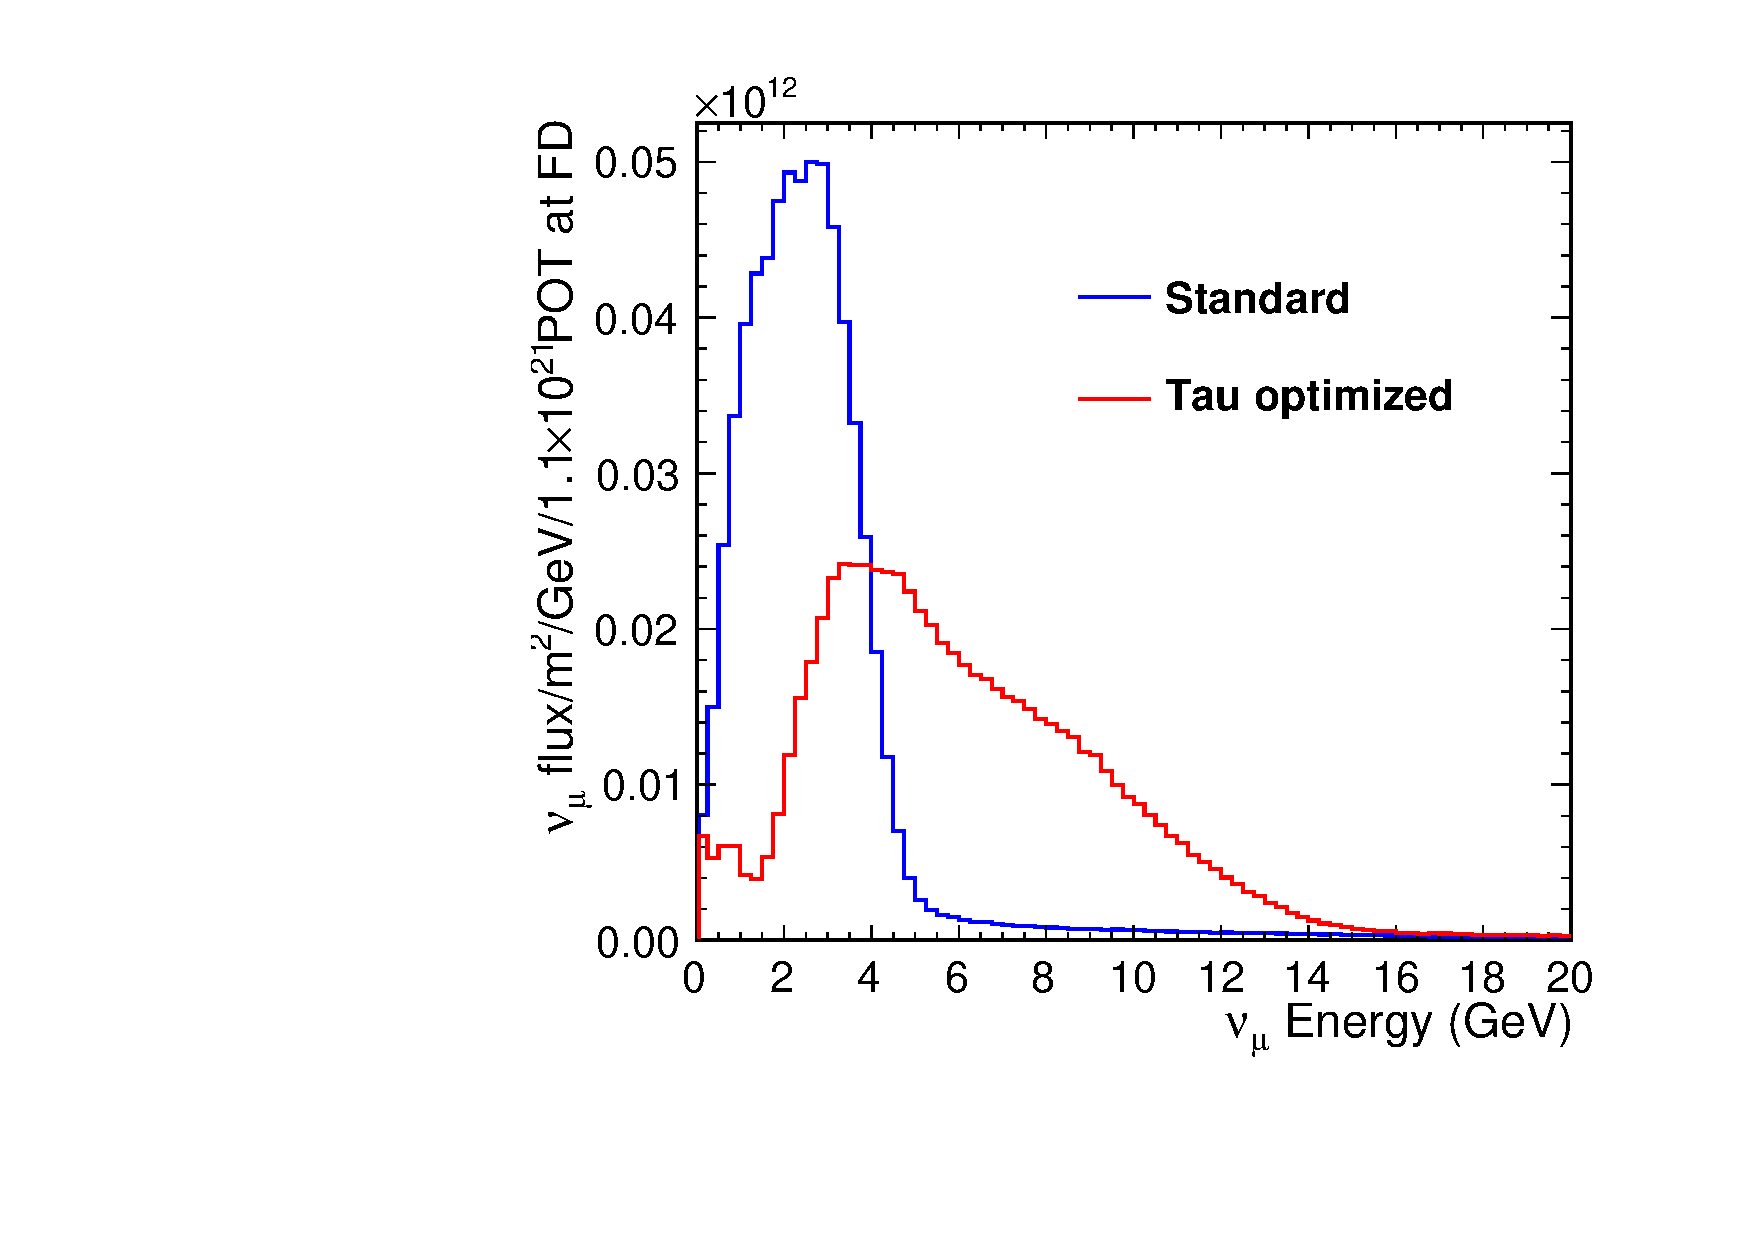
\includegraphics[width=0.5\textwidth]{tau_vs_nominal_neutrino_fd.pdf}
\end{dunefigure}

%\fixme{figure To be updated}



%%%%%%%%%%%%%%%%%%%%%%%%%%%%%%%
\subsection{Neutrino Interaction Generators} 
\label{sec:tools-mc-gen}

%\begin{itemize}
%\item Have this section owned by a Genie expert. Costas?
%\end{itemize}

%Both the beam neutrinos and atmospheric neutrinos were simulated using {\sc genie} v2\_10\_6. The beam neutrinos were simulated using the reference flux. We simulated unoscillated samples in both the neutrino and antineutrino modes. We also simulated fully oscillated samples where we convert all $\nu_\mu$'s in the beam to either $\nu_e$'s or $\nu_\tau$'s. 

%The atmospheric neutrinos were simulated using the Bartol flux for the Soudan site~\cite{ref:bartol}. There is a plan to use the Honda flux for the Homestake site~\cite{ref:honda} when the {\sc genie} flux interface is updated. 

\subsubsection{Supernova Neutrinos}

The \dword{snb} neutrino events were generated using custom code wrapped in a \dword{larsoft} module.
This code simulates \dword{cc} $\nu_e$-$^{40}$Ar interactions.
For each electron neutrino it calculates probabilities to produce a $^{40}$K nucleus
in different excited states (using a model from~\cite{Bhattacharya:1998hc}),
randomly selects one, and (with energy levels from~\cite{Cameron:2004myb}) 
produces several de-excitation $\gamma$s and an electron carrying the remaining energy.
All particles are produced isotropically, and 
there is no delay between the electron and corresponding de-excitation $\gamma$s
(in this model the $^{40}$K nucleus de-excites instantaneously) and they share a vertex,
which is simulated with equal probability anywhere in the active volume.
The primary neutrino energy distribution used in these samples is the cross-section-weighted 
energy spectrum obtained from SNOwGLoBES~\cite{snowglobes} (using the ``GKVM'' flux~\cite{GKVM}).
The \dword{snb} neutrino generator also allows to simulate a Poisson-distributed random number 
of neutrino interactions per event. These samples were simulated with, on average, 2 or 20 neutrinos.
In addition, one of the samples was generated with $1.01$~Bq/kg of $^{39}$Ar background.

\subsubsection{GENIE}

The DUNE \dword{mc} simulation chain is interfaced to the \dword{genie} event generator \cite{Andreopoulos:2009rq}. This is an open-source product of the \dword{genie} collaboration\footnote{www.genie-mc.org}  that provides state-of-the-art modeling of neutrino-nucleus interactions, as well as simulation of several other non-neutrino processes (nucleon decay, neutron-antineutron oscillation, boosted dark matter interactions, hadron and charged lepton scattering off nuclei). The generator product also includes off-the-shelf components (flux drivers and interfaces to outputs of detailed neutrino beamline simulations, detector geometry drivers, and several specialized event generation applications) for the simulation of realistic experimental setups. The \dword{genie} collaboration performs an advanced global analysis of neutrino scattering data, and is leading the development and characterization of comprehensive interaction models. The \dword{genie} comprehensive models and physics tunes which are developed using its proprietary Comparisons and Tuning products, are fully integrated in the \dword{genie} Generator product. Finally, the open-source \dword{genie} Reweight product provides means for propagating modeling uncertainties. 

At the time of the \dword{tdr} writing, the DUNE simulation uses a version in the v2 series of the \dword{genie} Generator, which includes empirical comprehensive models, based on home-grown hadronic simulations (AGKY model \cite{Yang:2009zx} for neutrino-induced hadronization and INTRANUKE/hA model \cite{Dytman:2015taa} for hadronic re-interactions) and nuclear neutrino cross sections calculated within the framework of the simple Relativistic Fermi Gas model \cite{Bodek:1981wr}. Several processes are simulated within that framework with the most important ones, in terms of the size of the corresponding cross section at a few GeV, being: (1) quasi-elastic scattering, simulated using an implementation of the Llewellyn Smith model \cite{LlewellynSmith:1971uhs}, (2) multi-nucleon interactions, simulated with an empirical model motivated by the Lightbody model \cite{Lightbody:1988gcu} and using a nucleon cluster model for the simulation of the hadronic system, (3) baryon resonance neutrino-production simulated using an implementation of the Rein-Sehgal model \cite{Rein:1980wg}, and (4) deep-inelastic scattering, simulated using the model of Bodek and Yang \cite{Bodek:2002ps}.  These comprehensive models, as well as the \dword{genie} procedure for tuning the cross section model in the transition region, have been used for several years and are well understood and documented \cite{Andreopoulos:2009rq}. The actual tune used is the one produced for the analysis of data from the MINOS experiment and, as it was already known at that time, it has several caveats as it emphasizes inclusive data and does not address tensions with exclusive data. The future DUNE simulation will be done using the v3 \dword{genie} Generator where improved models and tunes are available. %These comprehensive models and tunes are now unsupported, as they are superseded by the substantially improved versions listed below. However, they are included in v3 as they provide a connection with a large body of neutrino interaction studies.

%Building a comprehensive model for the simulation of neutrino interactions in the energy range of interest to current and near-future experiments poses significant challenges. This broad energy range bridges the perturbative and non-perturbative pictures of the nucleon and a variety of scattering mechanisms are important. In many areas, including elementary cross sections, hadronization models, and nuclear physics, one is required to piece together models with different ranges of validity in order to generate events over all of the available phase space. This inevitably introduces challenges in merging and tuning models, making sure that double counting and discontinuities are avoided. In addition, there are kinematic regimes which are outside the stated range of validity of all available models, in which case we are left with the challenge of developing our own models or deciding which model best extrapolates into this region. 
%
%At the time of writing this document, Generator v3.0.0 was the most recent version released by the GENIE Collaboration [(1) Paper on GENIE3 in progress -- Will provide reference ASAP]. This version includes several new, state-of-the-art comprehensive models and tunes, whose performance against a large collection of neutrino, charged-lepton and hadron scattering data was characterised in detail [(2) Paper with detailed model characterization in progress -- Will provide reference ASAP]. The following comprehensive models and tunes are currently available:
%
%{\bf G00\_00a\_00\_000} and {\bf G00\_00b\_00\_000}: They are equivalent to the historical ``Default'' and``Default+MEC'' models, as they were implemented in the latest releases of the v2 series of the GENIE Generator. They are empirical comprehensive models, based on home-grown hadronic simulations (AGKY model \cite{Yang:2009zx} for neutrino-induced hadronization and INTRANUKE/hA model \cite{Dytman:2015taa} for hadronic re-interactions) and nuclear neutrino cross-sections calculated within the framework of the simple Relativistic Fermi Gas model \cite{Bodek:1981wr}. Several processes are simulated within that framework with the most important ones, in terms of the size of the corresponding cross-section at few-GeV, being: a) quasi-elastic scattering, simulated using an implementation of the Llewellyn Smith model \cite{LlewellynSmith:1971uhs}, b) multi-nucleon interactions, simulated with an empirical model motivated by the Lightbody model \cite{Lightbody:1988gcu} and using a nucleon cluster model for the simulation of the hadronic system, c) baryon resonance neutrino-production simulated using an implementation of the Rein-Sehgal model \cite{Rein:1980wg}, and d) deep-inelastic scattering, simulated using the model of Bodek and Yang \cite{Bodek:2002ps}.  These comprehensive models, as well as the GENIE procedure for tuning the cross-section model in the transition region, have been used for several years and are well understood and documented \cite{Andreopoulos:2009rq}. The actual tune used is the one produced for the analysis of data from the MINOS experiment and, as it was already known at that time, it has several caveats as it emphasises inclusive data and does not address tensions with exclusive data. These comprehensive models and tunes are now unsupported, as they are superseded by the substantially improved versions listed below. However, they are included in v3 as they provide a connection with a large body of neutrino interaction studies.
%
%{\bf G18\_01a\_02\_11a} and {\bf G18\_01b\_02\_11a}: They are adiabatically improved versions of the historical comprehensive models. They include new processes (diffractive production of pions, hyperon production) and major upgrades to the final-state hadronic re-interaction models (the `01a' version uses the INTRANUKE/hA2018 hadronic re-interaction model, whereas `01b' uses the INTRANUKE/hN2018 model) [(1) Paper on GENIE3 in progress], but leave the base cross-section model unchanged with respect to the historical model. However, the cross-section model was re-tuned to deuterium data and shows much improved agreement with several exclusive $1\pi$ and $2\pi$ channels, while it maintained good agreement with inclusive data. [(3) Paper on tunes in progress -- Will provide reference ASAP]
%
%{\bf G18\_02a\_02\_11a} and {\bf G18\_02b\_02\_11a}: They are improved empirical models that share many of the features of G18\_01a\_02\_11a and G18\_01b\_02\_11a (new processes, improved hadronic simulations, new tunes), but introduced changes to the base cross-section model. In these comprehensive models, the Rein-Sehgal coherent and resonance neutrino-production models \cite{Rein:2006di, Rein:1980wg} were replaced with the better-motivated models produced by Berger-Sehgal \cite{Berger:2008xs, Berger:2007rq}.
%
%{\bf G18\_10a\_02\_11a} and {\bf G18\_10b\_02\_11a}: They are comprehensive models anchored on the best theory currently impleented in GENIE. They are similar to G18\_02a\_02\_11a and G18\_02b\_02\_11a, respectively, but for the simulation of quasielastic-like processes they implement a modern microscopic calculation by the Valencia group. Quasi-elastic processes, within a Local Fermi Gas (LFG) model and simulating Coulomb and Random Phase Approximation (RPA) corrections are implemented based on Ref. \cite{Nieves:2004wx}, whereas 2p2h processes are implemented based on Ref. \cite{Nieves:2011pp}.
%
%{\bf G18\_10i\_00\_000} and {\bf G18\_10j\_00\_000}: They are similar to G18\_10a\_02\_11a and G18\_10b\_02\_11a, but using the better-motivated $z$-expansion \cite{Hill:2010yb} of the axial form factor. However, due to extra complications in incorporating deuterium experiment flux constraints when using the $z$-expansion model in the GENIE tunes, both of these comprehensive models were untuned in v3.0.0, though a tune will be made available in a future revision. 

Besides simulation of neutrino-nucleus interactions, \dword{genie} provides simulation of several \dword{bsm} physics channels:

\textit{\dword{bsm}}: The implementation of a \dword{bsm} \dword{mc} simulation has been motivated by several theory studies \cite{Agashe:2014yua,Berger:2014sqa, Kong:2014mia, Cherry:2015oca, Kopp:2015bfa, Necib:2016aez, Alhazmi:2016qcs,Kim:2016zjx}. The current implementation focuses on two models presented in  \cite{Berger:2014sqa}. The first has a fermionic \dword{dm} candidate, a $Z^\prime$ mediator, and a $u^0$ velocity dependence of the spin-dependent cross section in the non-relativistic limit. The second model has a scalar \dword{dm} candidate, a $Z^\prime$ mediator, and a $u^2$ velocity dependence of the spin-dependent cross section in the non-relativistic limit.

\textit{Nucleon decay}: \dword{genie} simulates several nucleon decay topologies. For the initial nuclear state environment and intranuclear hadron transport, it uses the same modeling as is does for neutrino event simulation. In the nucleon decay simulation, the nucleon binding and momentum distribution is simulated using one of the nuclear models implemented in \dword{genie} (typically a Fermi Gas model), and it is decayed to one of many topologies using a phase space decay. The decay products are produced within the nucleus and further re-interactions of hadrons are simulated by the \dword{genie} hadron transport models. The simulated nucleon decay topologies are given in Table~\ref{tab:genie_ndk}, presented in the Appendix
in Sec.~\ref{sec:tools-app-generator}.

\textit{Neutron-antineutron oscillation}: \dword{genie} simulates several event topologies that may emerge following the annihilation of the antineutron produced from a bound neutron to antineutron transition. For the initial nuclear state environment and intranuclear hadron transport, the simulation, as in the case of nucleon decay, uses the same modeling as  is does for the neutrino event simulation. The simulated reactions are listed in Table~\ref{tab:nnbar-br} in 
Sec.~\ref{subsec:nonaccel-nnbar-dunesensitivity}.


%%%%%%%%%%%%%%%%%%%%%%%%%%%%%%%
\subsection{Detector Simulation}
\label{sec:tools-mc-detsim}

%\begin{itemize}
%\item Charged particle-argon interactions
%\item Radiologicals
%\begin{itemize} \item Table from Jason Stock \end{itemize}
%\item Geometries
%\begin{itemize} \item Figure showing ProtoDUNE, 1x2x6 \end{itemize}
%\item LArG4
%\item Photon Simulation
%\begin{itemize}
%\item LAr optical properties
%\item Photon Library (or replacement) method
%\item Photon library figure
%\end{itemize}
%\item TPC detector signal simulation (Xin et al.)
%\end{itemize}

\subsubsection{LArG4}\label{sec:larg4}

The truth particles generated in the event generator step are passed to a {\sc geant4} v4\_10\_1\_p03-based detector simulation. In this step, each primary particle from the generator and its decay or interaction daughter particles are tracked when they traverse \lar. The energy deposition is converted to ionization electrons and scintillation photons. Some electrons are recombined with the positive ions~\cite{Acciarri:2013met,Amoruso:2004dy} while the rest of the electrons are drifted towards the wire planes. The number of electrons is further reduced due to the existence of impurities in the \lar, which is commonly parameterized as the electron lifetime. The default electron lifetime is \SI{3}{ms} in the simulation. The longitudinal diffusion smears the arrival time of the electrons at the wires and the transverse diffusion smears the electron location among neighboring wires. More details
regarding the recent measurements of diffusion coefficients can be found
in~\cite{Li:2015rqa,larpropertiesbnl}.

\subsubsection{Photon Simulation}

When ionization is calculated, the amount of scintillation light is also calculated. The response of the \dwords{pd} is simulated using a ``photon library,'' a pre-generated table giving the likelihood that photons produced within a voxel in the detector volume  will reach any of the \dwords{pd}. The photon library is generated using \dword{geant4}'s photon transport simulation, including \SI{66}{cm} scattering length, \SI{20}{m} attenuation length, and reflections off of the interior surface detectors. The library also incorporates the response versus location of the \dwords{pd}, capturing the attenuation between the initial conversion location of the photon and the \dwords{sipm}.

\subsubsection{TPC Detector Signal Simulation}\label{sec:tpc_sim}

When ionization electrons drift through the induction wire planes toward the collection wire plane, current is
induced on nearby wires. The principle of current induction is described by the Ramo theorem~\cite{Shockley1938,Ramo:1939vr}. 
For an element of ionization charge, the instantaneous induced current $i$ is proportional to the amount of drifted charge $q$: 
\begin{equation}\label{eq:shockley_ramo}
  i = - q \cdot \vec{E}_w \cdot \vec{v}_q.
\end{equation}
The proportionality factor is a product of the weighting field $\vec{E}_w$ at the location of the charge and 
the charge's drifting velocity $\vec{v}_q$. The weighting field $\vec{E}_w$ depends on the geometry of 
the electrodes. The charge's drifting velocity $\vec{v}_q$ is a function of the external \efield, which 
also depends on the geometry of the electrodes as well as the applied drifting and bias voltages. The current induced at a given electrode and electron drift path ($x$)
  sampled over a period of time ($t$) is called a ``field response function'' $R(x,t)$.

\begin{figure}[!htp]
\centering
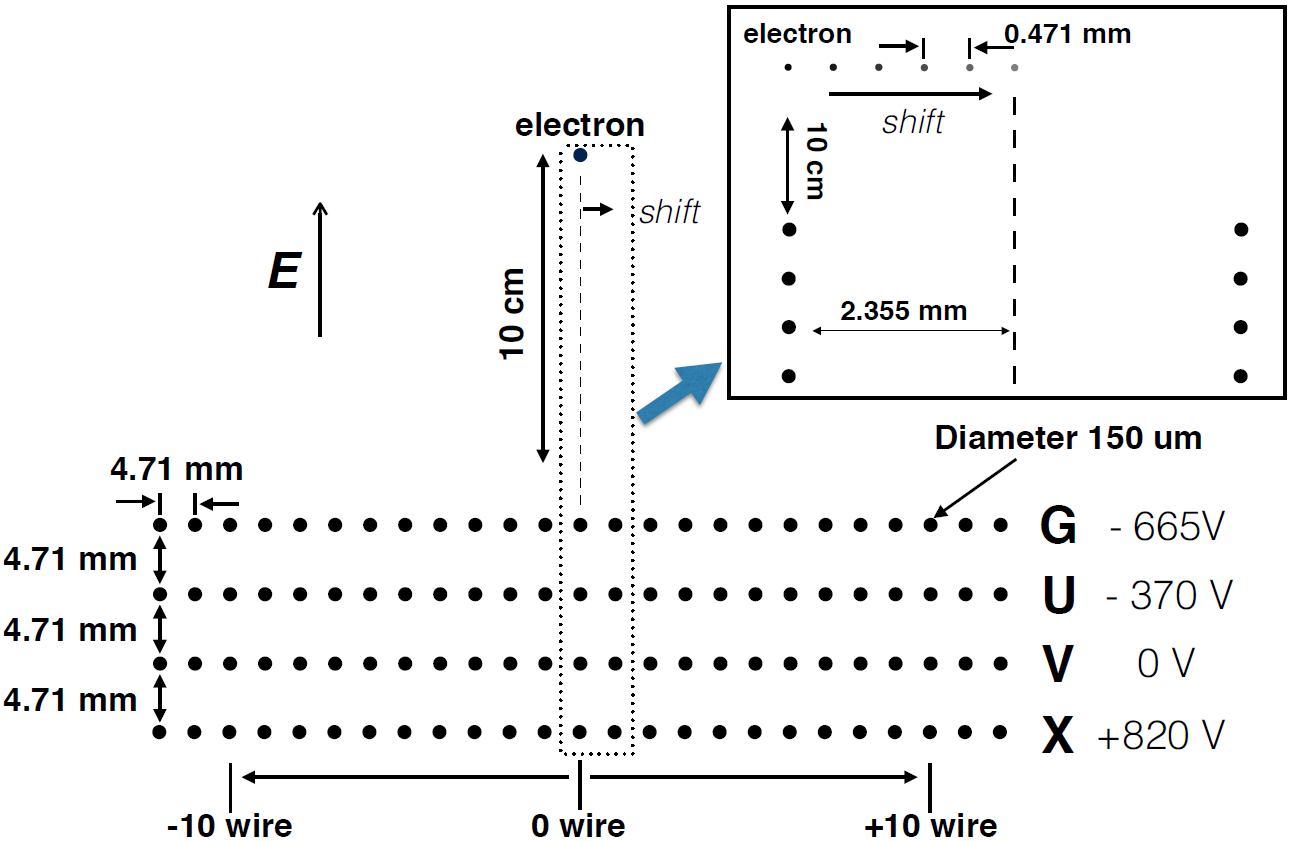
\includegraphics[width=0.85\textwidth]{apa_cell.png}
\caption[Garfield configuration for simulating the field response functions]{Garfield configuration for simulating the field response functions.}
\label{field_resp_geometry}
\end{figure}

The field response functions for a single ionization electron are simulated with Garfield~\cite{garfield}. \fixme{add to glossary?} 
In the Garfield simulation, a region with \SI{22}{cm} (along the \efield or drift direction) $\times$ 
\SI{30}{cm} (perpendicular to the field direction and wire orientation) is configured as shown in 
Figure~\ref{field_resp_geometry}. There are five wire planes with \SI{4.71}{mm} spacing, referred to as G, U, V, X, and 
M with operating bias voltages of \SI{-665}{V}, \SI{-370}{V}, \SI{0}{V}, \SI{820}{V}, \SI{0}{V}, respectively.  
These bias voltages ensure 100\% transmission of electrons through the grid plane (G) and the 
first two induction planes (U and V) and complete collection by the collection plane X with the main drift 
field at \SI{500}{V/cm}. In the simulation, each wire plane contains 101 wires with \SI{150}{\micro\meter} diameter
  separated at $\sim\,$\SI{4.71}{\mm} wire pitch. The electron drift velocity as a function of electric
  field is taken from recent measurements~\cite{Li:2015rqa,larpropertiesbnl}. 

 \begin{figure}[!htp]
  \centering
  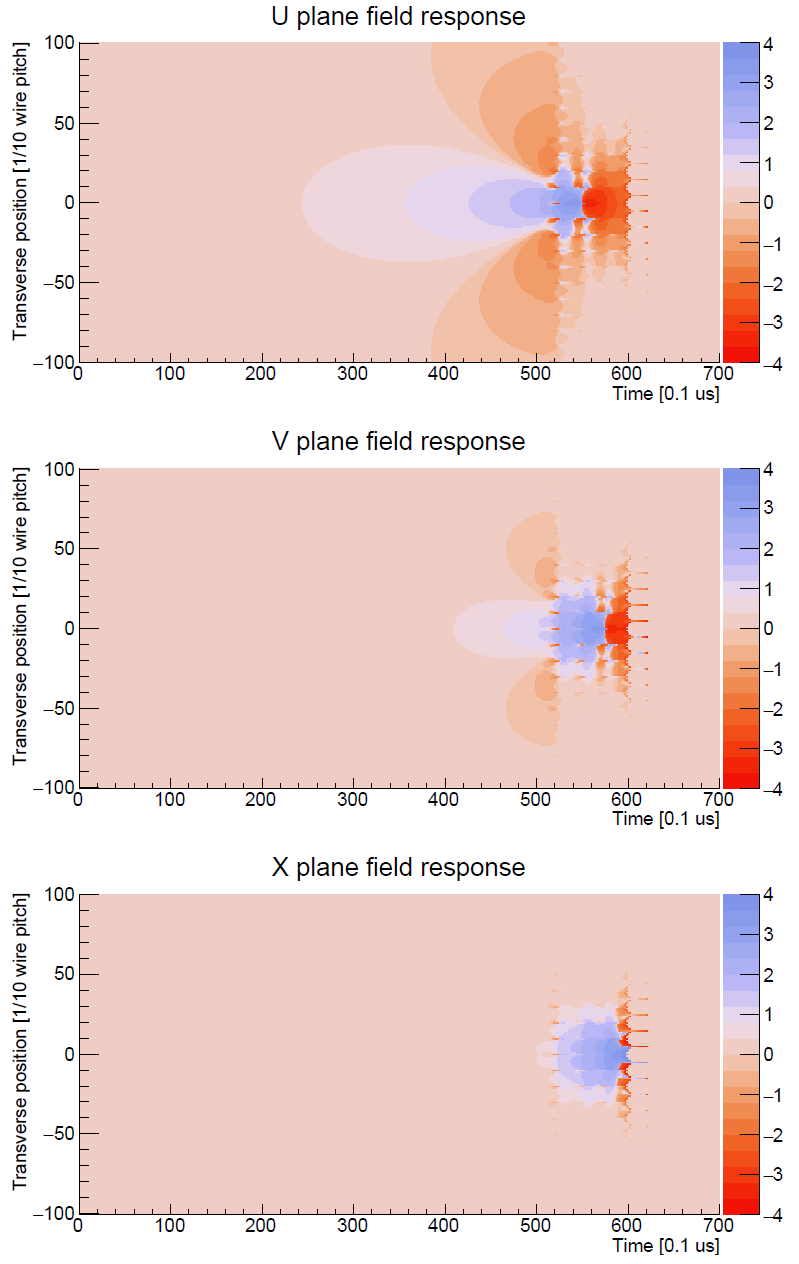
\includegraphics[width=0.7\textwidth]{field_response_data.png}
\caption[Position-dependent field response simulated with the Garfield program]{Position-dependent field response simulated with the Garfield program 
for two induction and one collection planes in the ``Log~10'' format. The wire of interest 
is assumed to locate at position zero. The ionization electron is assumed at different
positions in the transverse direction. See text for more discussion.}
\label{field_resp}
\end{figure}

 Given the above configuration, the field response function can then be calculated in Garfield
  for each individual wire  for an
  electron starting from any position within the region of simulation. 
  The field response functions for $\pm\,$10 wires on both sides of the central wire (21 wires in total) are 
  recorded. In addition to this position, five other positions with
  \SIlist{0.471;0.942;1.413;1.884;2.355}{\mm} horizontal shift towards one direction are also simulated.
  In total, 126 field responses (six positions for 21 readout wires) are calculated for each wire plane and stored for later
  application in the TPC detector signal simulation.
  Figure~\ref{field_resp} shows the simulated field response ($i$ in $\mu A$ with 0.1 $\mu s$ time bin) 
   in the ``Log~10'' format:
   \begin{equation}\label{eq:log10}
    i \text{ in ``Log 10'' } =
    \begin{cases}
      \text{log}_{10}(i\cdot4\times10^{10}),& \text{if }i>2.5\times10^{-11},\\
      0,& \text{if }  -2.5 \times10^{-11} \leq i \leq 2.5 \times 10^{-11},\\
      -\text{log}_{10}(- i\cdot4\times10^{10})& \text{if }i<-2.5\times10^{-11}.\\
      \end{cases}
  \end{equation}
  
  Following the earlier work in MicroBooNE~\cite{Adams:2018dra}, the TPC detector signal simulation
  is implemented in the software package Wire-Cell Toolkit~\cite{ref:wire_cell_toolkit,ref:full_simulation}, which is 
  further interfaced with \dword{larsoft}. This simulation procedure has been validated in the MicroBooNE experiment~\cite{Adams:2018gbi}. In
  the following, we summarize the major features. The TPC signal simulation takes input from the \dword{geant4}-simulated energy deposition when particles traverse the detector, and outputs digitized waveforms on the \dword{fe} electronics.
   A data-driven, analytical simulation of the inherent electronics noise is also performed. 
Figure~\ref{fig:simevent_wf} shows the example waveform for minimum ionizing particles traveling parallel to 
the wire plane, but perpendicular to the wire orientation.  Figure~\ref{fig:simevent} shows one example event of 
a \dword{mip} traveling through one \dword{apa}. 

\begin{figure}[htbp]
  \centering
        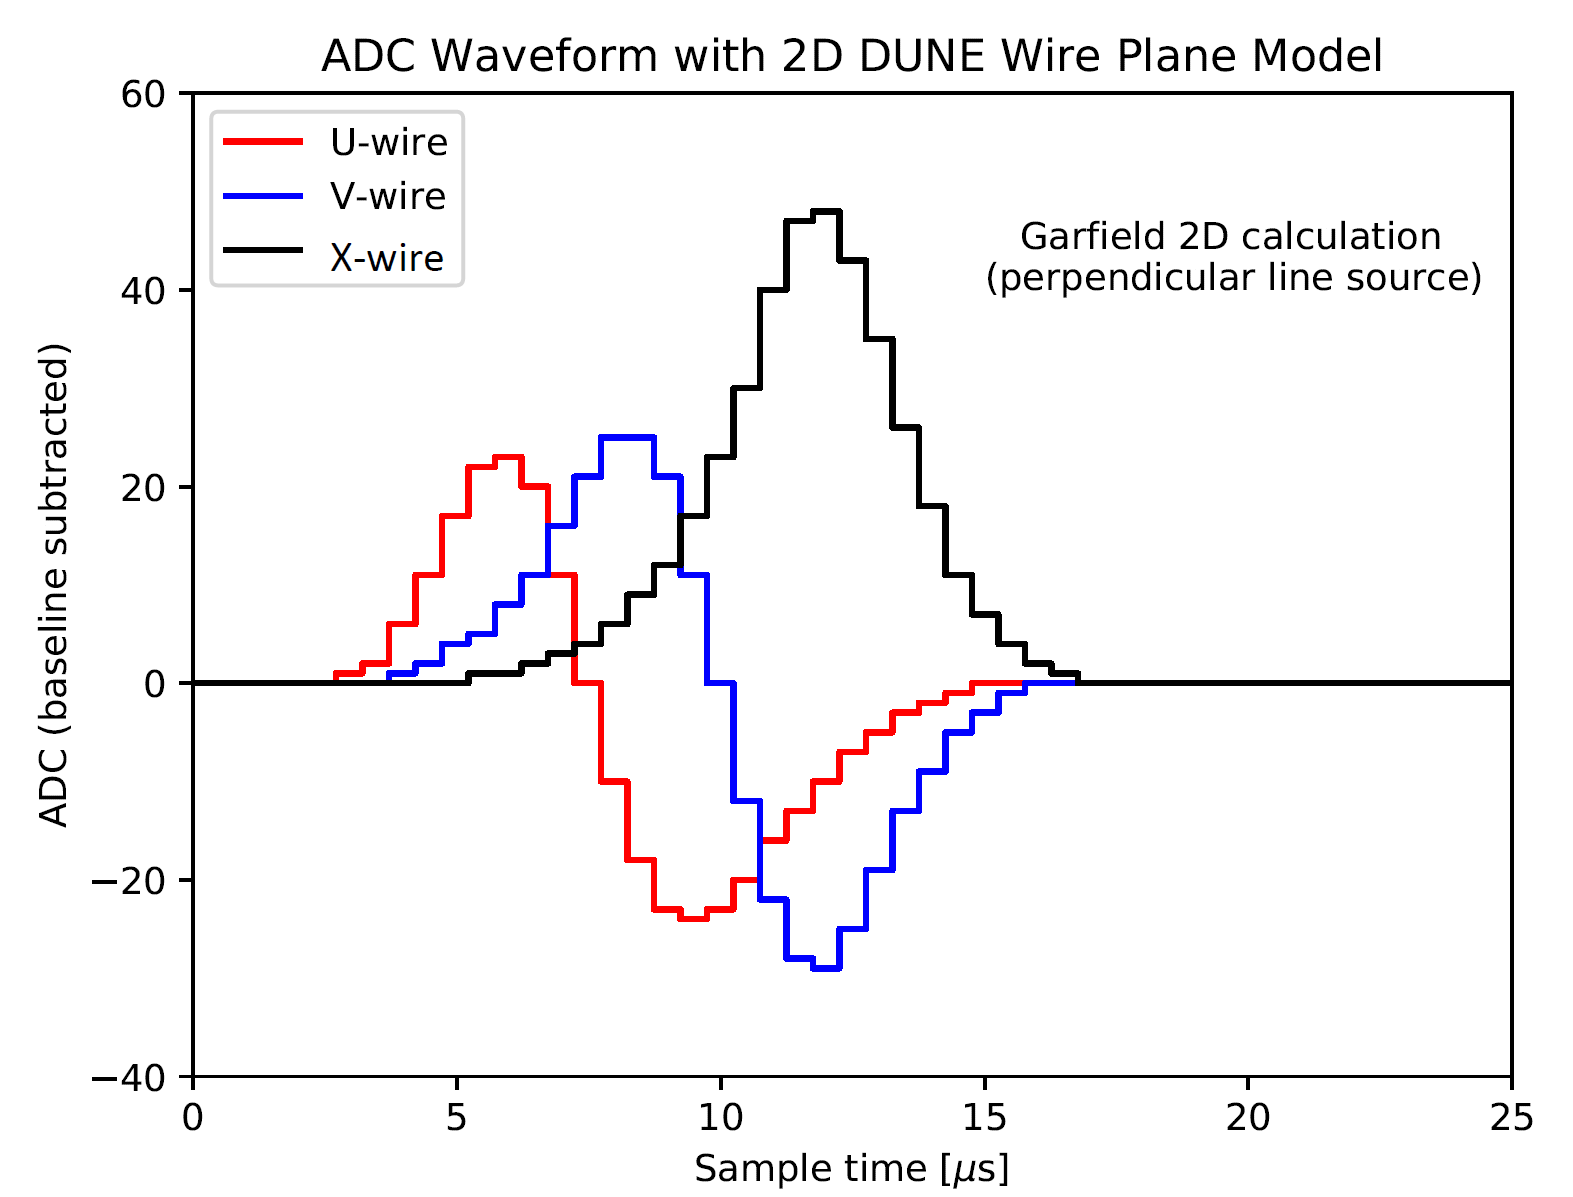
\includegraphics[width=0.6\textwidth]{DUNE_line_source_wf.png}
        \caption{Waveform for minimum ionizing particles traveling parallel to the wire plane. For different
        wire plane, the corresponding track is assumed to travel perpendicular to the wire orientation. 
        }\label{fig:simevent_wf}
         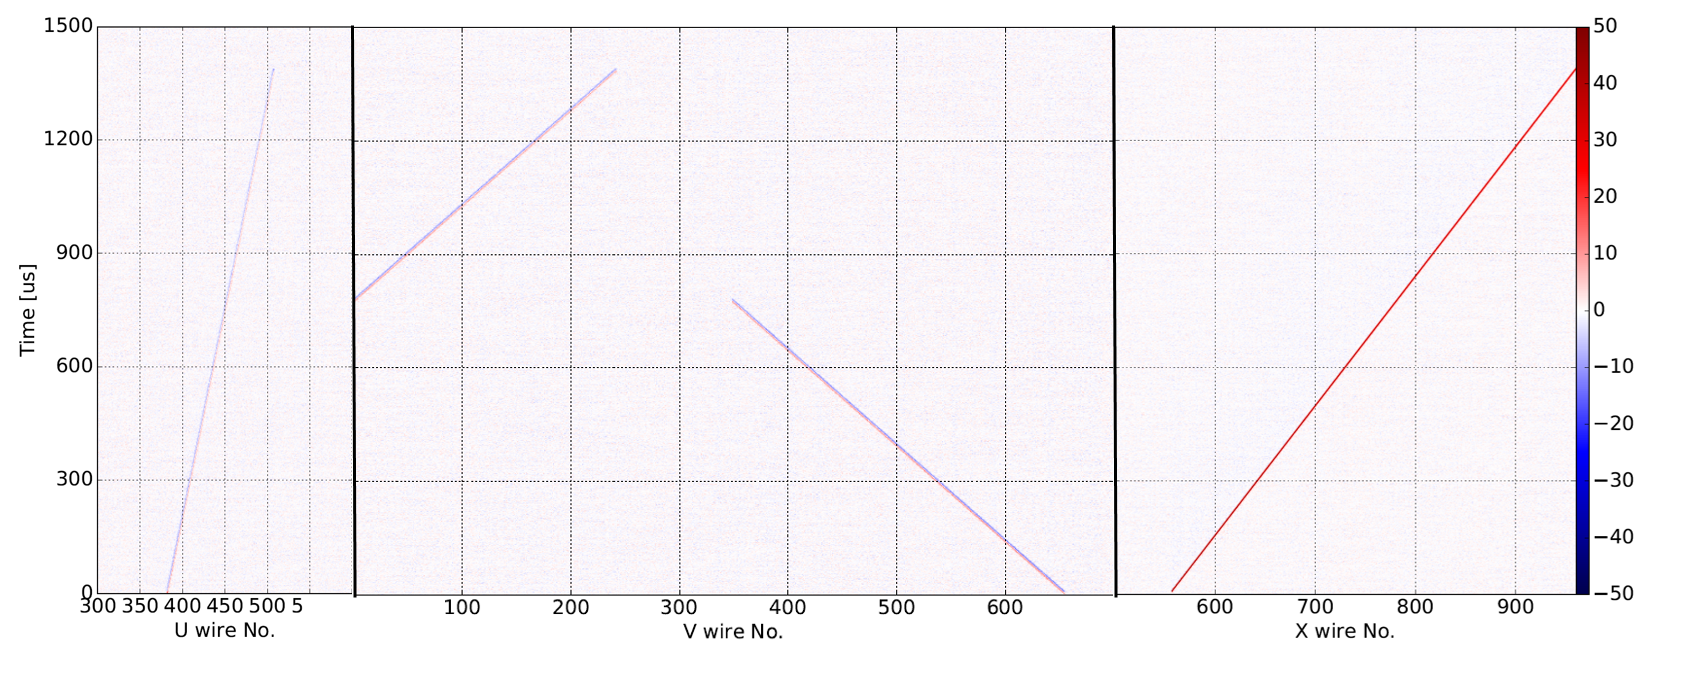
\includegraphics[width=0.95\textwidth]{track_sim.png}
    \caption{Simulated waveform for a \dword{mip} traveling through one \dword{apa}. The discontinuity of the 
    tracks in the V plane is caused by the wrapped wires.}
  \label{fig:simevent}
\end{figure}

The signal simulation, i.e., the \dword{adc} waveform on a given channel, 
\begin{equation}
  \label{eq:sim-convolution}
    M = (Depo \otimes Drift \otimes Duct + Noise) \otimes Digit, 
\end{equation}
%\footnote{symbol $\otimes$: circular convolution, also known as cyclic convolution or periodic convolution, arises in the context of the discrete-time Fourier Transform (DTFT).}
is conceptually a convolution of five functions:
\begin{description}
\item[$Depo$] represents the initial distribution of the ionization electrons created by energy depositions in space and time as
discussed in Section~\ref{sec:larg4}.
\item[$Drift$] represents a function that transforms an initial charge cloud to a distribution of electrons arriving at the wires. Physical processes related to drifting, including attenuation due to impurities, diffusion and possible distortions to the nominal applied \efield, are applied in this function.
\item[$Duct$] is a family of functions, each is a convolution $F \otimes E$ of the field response functions $F$ associated with the sense wire and the element of drifting charge and the electronics response function $E$ corresponding to the shaping and amplification of the \dword{fe} electronics. More details can be found in Section~\ref{sec:tools-mc-daq}.
\item[$Digit$] models the digitization electronics according to a given sampling rate, resolution, and dynamic voltage range and baseline offset resulting in an \dword{adc} waveform. 
\item[$Noise$] simulates the inherent electronics noise by producing a voltage level waveform from a random sampling of a Rayleigh distributed amplitude spectrum and uniformly distributed phase spectrum.  The noise spectra used are from measurements with the \dword{pdsp} detector after software noise filters, which have excess (non-inherent) noise effects removed.
\end{description}
%
These functions are defined over broad ranges and with fine-grained resolution. The resolutions are set by the variability (sub millimeter) and extent (several centimeters) of the field response functions and the sampling rate of the digitizer (\SI{0.5}{\micro\second}). Their ranges are set by the size of the detector (several meters) and the length of time over which one exposure is digitized (several milliseconds).  


%%%%%%%%%%%%%%%%%%%%%%%%%%%%%%%
\subsection{Data Acquisition Simulations and Assumptions}
\label{sec:tools-mc-daq}

%\begin{itemize}
%\item TPC electronics and noise simulation (Xin et al.) 
%\begin{itemize} \item Signal simulation/processing figure \end{itemize}
%\item Photon detector electronics simulation
%\end{itemize}

  The electrons on each wire are converted into raw wire signal (\dword{adc} vs Time) by convolution with the field response and electronics response. The \dword{asic} electronics response was simulated with the BNL SPICE~\cite{spice} simulation.  For most samples, the \dword{asic} gain was set to \SI{14}{mV/fC} and the shaping time was set to \SI{2}{\micro\second}. For the samples generated with 3 mm wire spacing, the \dword{asic} gain was set to \SI{25}{mV/fC}. The noise level was set to around 2.5 \dword{adc} RMS,based on extrapolation 
  from MicroBooNE experiment~\cite{Acciarri:2017sde}. This value was further validated in \dword{pdsp}. % experiment.
  Figure~\ref{elec_resp} shows the expected electronics shaping functions.

\begin{figure}[!h!tbp]
\centering
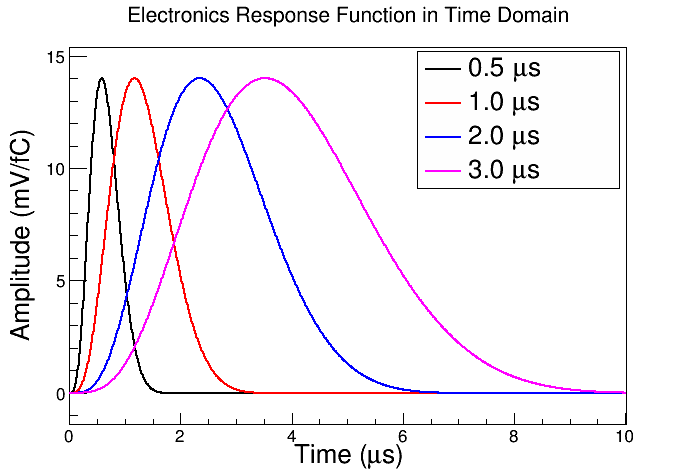
\includegraphics[width=0.7\textwidth]{elec.png}
\caption[\dword{asic}'s electronics shaping functions]{\dword{asic}'s electronics shaping functions
are shown for four shaping time settings at \SI{14}{mV/fC} gain.}
\label{elec_resp}
\end{figure}


The \dword{pd} electronics simulation separately generates waveform 
for each channel (\dword{sipm}) of a \dword{pd} that has been hit by photons.
Every detected photon %that has been detected 
appears as a single \phel{} pulse
(with the shape taken from~\cite{http://lss.fnal.gov/archive/2015/pub/fermilab-pub-15-488-nd-ppd.pdf:2015gov}) on a randomly selected channel
(belonging to the \dword{pd} in which the photon was registered).
Then dark noise (with the rate of \SI{10}{Hz}) and 
line noise (Gaussian noise with the RMS of $2.6$ \dword{adc} counts) are added.
Each photon (or a dark-noise pulse) has a probability of appearing
as $2$ \phel{}s on a waveform (the cross-talk probability is $16.5~\%$).
The final step of the digitization process is recording only fragments
of the full simulated waveform that have a signal in them.
This is accomplished by passing the waveform through a hit finder
described in Sec.~\ref{sec:gaushit} 
and storing parts of the waveform corresponding to the hits found.


%%%%%%%%%%%%%%%%%%%%%%%%%%%%%%%%%%%%%%%%%%%%%%%%%%%%%%%%%%%%%%%%
\section{Event Reconstruction in the \dword{fd}}
\label{sec:tools-fdreco}

This section describes various reconstruction algorithms used to reconstruct events in the \dword{fd} TPC. A successful \lartpc reconstruction needs to deliver reconstructed tracks and showers, particle and event identification, particle momentum and event energy. The reconstruction starts with finding signals on each wire above a threshold and building ``hits'' out of each pulse. All the LArTPC \threed reconstruction algorithms share the same principle. The $x$ coordinate is determined by the drift time and the $y$ and $z$ coordinates are determined by the intersection of two wires on different planes with coincident hits. There are currently three different reconstruction approaches in the DUNE reconstruction package. The \twod$\rightarrow$\threed reconstruction approach starts with clustering together nearby hits on each plane, %together 
followed by the use of time information to match \twod clusters between different planes to form \threed tracks and showers. Examples of this approach include TrajCluster and \dword{pandora}.  The direct \threed approach reconstructs \threed points directly from hits and then proceeds to perform pattern recognition using those \threed points. Examples of this approach include SpacePointSolver and \dword{wirecell}. The third approach uses a deep-learning technique, known as a \dword{cnn}. There are several tools needed to complete the task of LArTPC reconstruction. These tools include track fitter (\dword{pma} or KalmanFilter), calorimetry, \dword{pid} and track momentum reconstruction using range for contained tracks or multiple Coulomb scattering for exiting tracks. In addition to the TPC reconstruction, the \dword{pd} reconstruction provides trigger and $t_0$ information for non-beam physics. 

%\begin{itemize}
%\item TPC reconstruction methods
%\begin{itemize}
%\item Demo figure for each method below
%\item TPC signal processing (Xin et al.)
%\item Hit reconstruction
%\item Track/Shower CNN
%\item TrajCluster
%\item PMA
%\item Pandora (Lorena)
%\item Wirecell (Xin et al.)
%\item SpacePointSolver
%\end{itemize}
%\item TPC Reco performance
%\begin{itemize} 
%\item Track finding efficiency vs. position, angle
%\item Shower purity/completeness comparison figures 
%\end{itemize}
%\item Photon detector reconstruction methods
%\begin{itemize}
%\item Hit finding
%\item Flash finding
%\begin{itemize} \item SN, PDK photon `event displays' \end{itemize}
%\item Calorimetry
%\end{itemize}
%\item Photon Reco Performance
%\begin{itemize}
%\item Efficiency vs. energy/position figures
%\item Timing resolution figure
%\item Energy resolution figure
%\end{itemize}
%\end{itemize}

\subsection{TPC Signal Processing}\label{sec:tpc_sp}

The raw data are in the format of \dword{adc} counts as a function of TPC ticks (\SI{0.5}{\micro\second} on each channel. The signal has a 
unipolar shape for a collection wire and a bipolar shape for an induction wire. The first step 
in the reconstruction is to reconstruct the distribution of ionization electrons arriving at anode plane. 
This is achieved by passing the raw data through a deconvolution algorithm. In real detectors, excess 
noise may exist and require removal %need to be removed 
through a dedicated noise filter~\cite{Acciarri:2017sde}. 

The deconvolution technique was introduced to LArTPC signal processing in the context ArgoNeuT 
data analysis~\cite{Baller:2017ugz}. The goal of the deconvolution is to ``remove'' the impact of field and 
electronics responses from the measured signal along the time dimension in order to reconstruct the number of ionized
electrons. This technique has the advantages of being robust and fast, and is an essential step in the overall drifted-charge profiling process. This 1D deconvolution procedure was improved to a \twod deconvolution procedure 
by the MicroBooNE collaboration~\cite{Adams:2018dra,Adams:2018gbi}, which further took into account the long-range 
induction effects in the spacial dimension. Two-dimensional software filters (channel and time) are implemented to 
suppress high-frequency noise after deconvolution procedure. For induction plane signals, regions of interest 
(ROIs) are selected to minimize the impact of electronics noise. More details of this algorithm can be found in~\cite{Adams:2018dra}.

This procedure, implemented in the \dword{wirecell} toolkit software package~\cite{ref:wire_cell_toolkit},  has been used in the TPC signal processing in \dword{pdsp}. Figure~\ref{pDUNE_sp_wf}
shows an example induction U-plane waveform before and after the signal processing procedure. The bipolar 
shape is converted into a unipolar shape after the \twod deconvolution. Figure~\ref{pDUNE_sp_example}
shows full \twod image of induction U-plane signal from a \dword{pdsp} 
event~\cite{ref:pdune_signal_processing}. The measured signal (left) has a bipolar shape with red (blue) color 
representing positive (negative) signals. The deconvolved signal after 
the \twod deconvolution procedure (right) represents the reconstructed 
distribution of ionization electrons arriving at anode wire plane. The 
deconvolved signal becomes unipolar, and the long-range 
induction effect embedded in the field response is largely removed. 


\begin{figure}[!h!tbp]
\centering
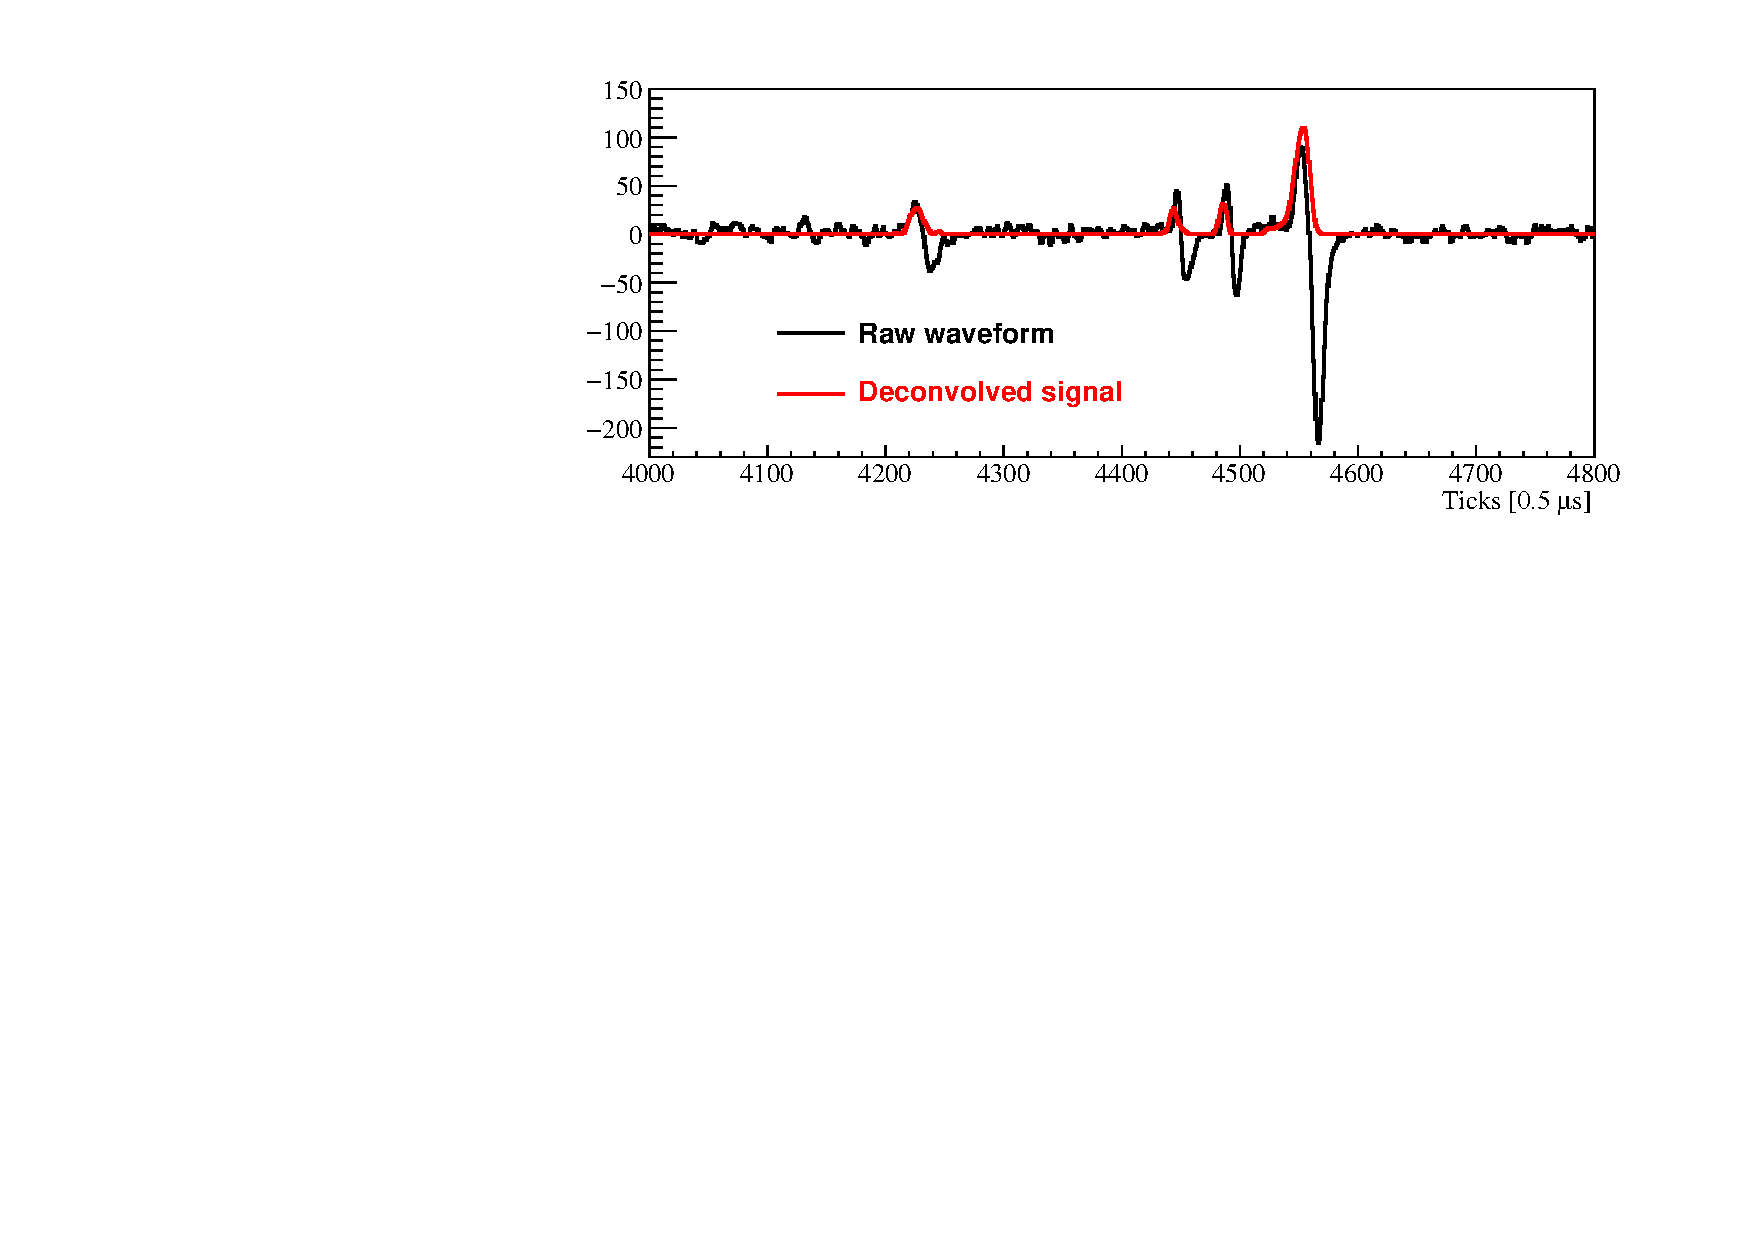
\includegraphics[width=0.95\textwidth]{sample_5141_23865.pdf}
\caption[Measured and deconvolved waveform from an induction U-plane channel of \dword{pdsp}]{An example of measured (black) and deconvolved waveform from an induction U-plane channel of \dword{pdsp}
before and after the signal processing procedure. For measured waveform, the unit is \dword{adc}. For deconvolved
waveform, the unit is number of electrons after scaling down by a factor of 125.
Bipolar signal shape is converted into a unipolar signal shape after \twod deconvolution.}
\label{pDUNE_sp_wf}
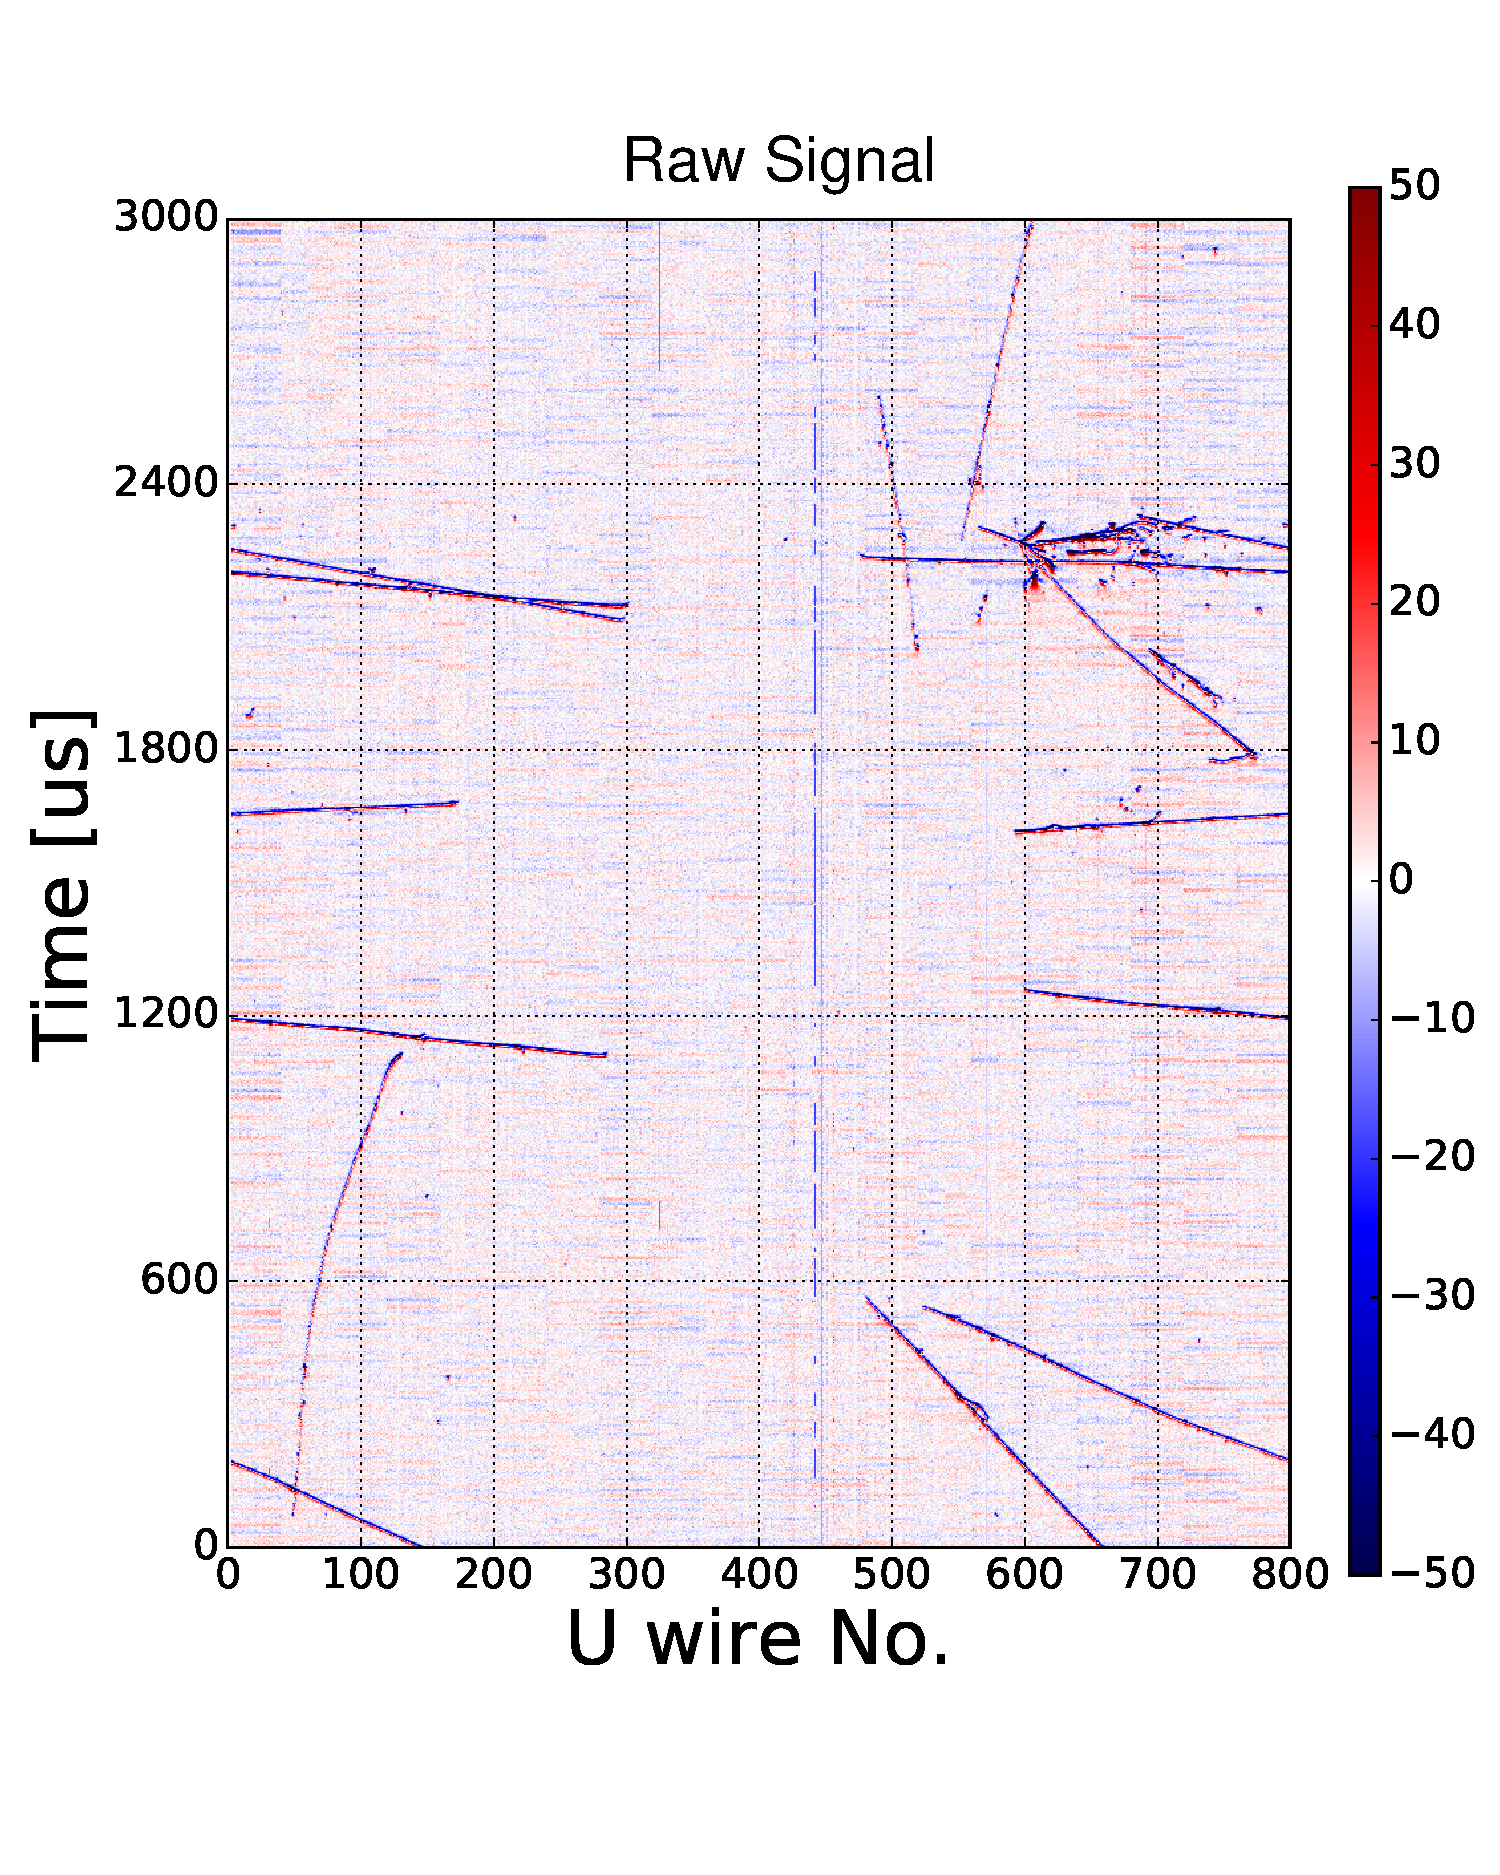
\includegraphics[width=0.49\textwidth]{protodune_raw_u.pdf}
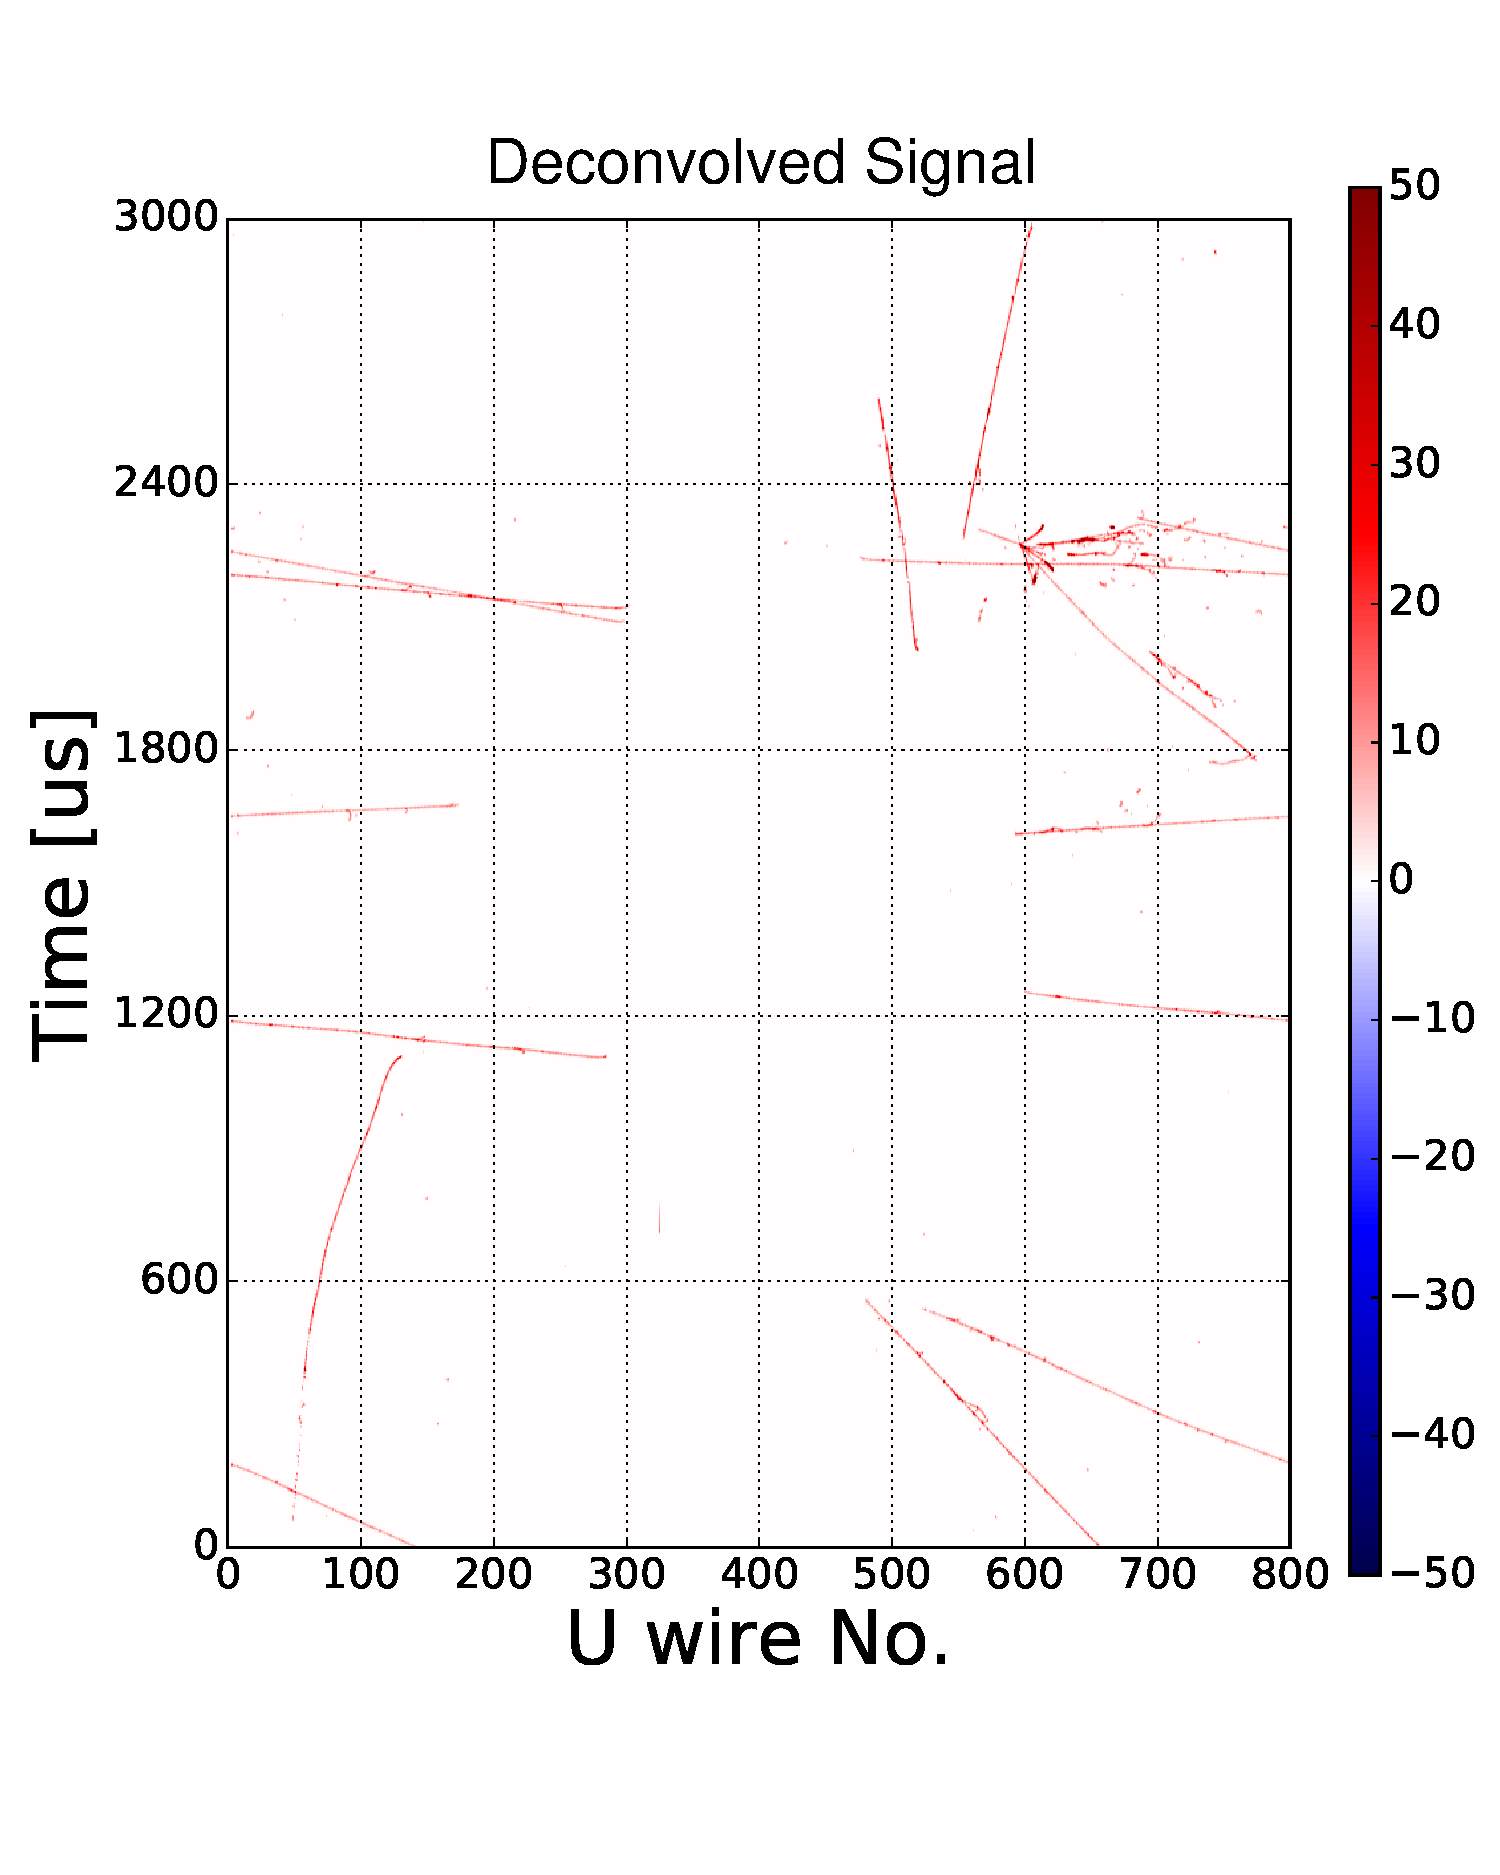
\includegraphics[width=0.49\textwidth]{protodune_decon_u.pdf}
\caption{Comparison of raw (left) and deconvolved induction U-plane signals (right) before and after 
the signal processing procedure from a \dword{pdsp} event. The bipolar shape with red (blue) color representing
positive (negative) signals is converted to the unipolar shape after the \twod deconvolution. }
\label{pDUNE_sp_example}
\end{figure}


\subsection{Hit and Space-Point Identification}

\subsubsection{Gaussian Hit Finder}\label{sec:gaushit}

The reconstruction algorithms currently employed by \larsoft are based on finding hits on the deconvolved waveforms for each plane. A key assumption is that the process of deconvolution will primarily result in gaussian shaped charged deposits on the waveforms and this drives the design of the gaussian hit finder module. Generally, the module loops over the input deconvolved waveforms and handles each in three main steps: first it searches the waveforms %are searched 
for candidate pulses, it then fits these candidates %are then fit 
to a gaussian shape and, finally, it places the resulting hit %is then placed 
in the output hit collection. Not all charge deposits will be strictly gaussian shaped, for example a track can emit a delta ray and it can take several wire spacings before the two charge depositions are %will be 
completely separated. Alternatively, a track can have a trajectory at large angles to the sense wire plane creating a charge deposition over a large number of waveform ticks. The candidate peak-finding stage of the hit finder attempts to resolve the individual hits in both of these cases, still under an assumption that the shape of each individual charge deposition is %will be 
gaussian. If this results in candidate peak trains that are ``too long'' then special handling  breaks these into a number of evenly spaced hits and bypasses the hit-fitting stage. 

Figure~\ref{pDUNE_sp_hits} displays the results of the gaussian hit finder for the case of two or three hits only barely separated in \dword{pdsp} data. In this figure the deconvolved waveform is shown in blue, the red line represents the fit of the candidate peak to two or three gaussian shapes, the crosses represent the centers of the fit peaks, the pulse heights above the waveform baseline and their fit widths. 
\begin{figure}[!h!tbp]
\centering
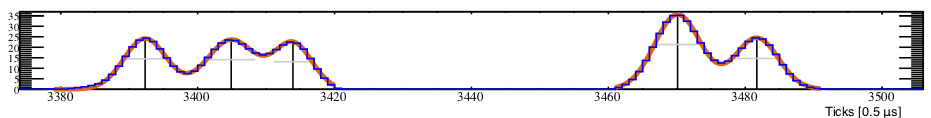
\includegraphics[width=\textwidth]{hits.png}
\caption[An example of reconstructed hits in \dword{pdsp} data]{An example of reconstructed hits in \dword{pdsp} data. The deconvolved waveform is shown in blue, the red line represents the fit of the candidate peak to two or three gaussian shapes, the crosses represent the centers of the fit peaks, the pulse heights above the waveform baseline and their fit widths.
}
\label{pDUNE_sp_hits}
\end{figure}

\subsubsection{Space Point Solver}

\begin{figure}
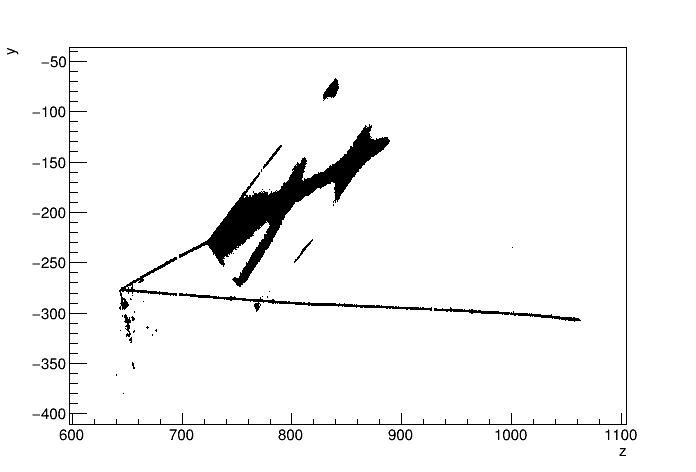
\includegraphics[width=.5\linewidth]{evd_zy_pre_2302}
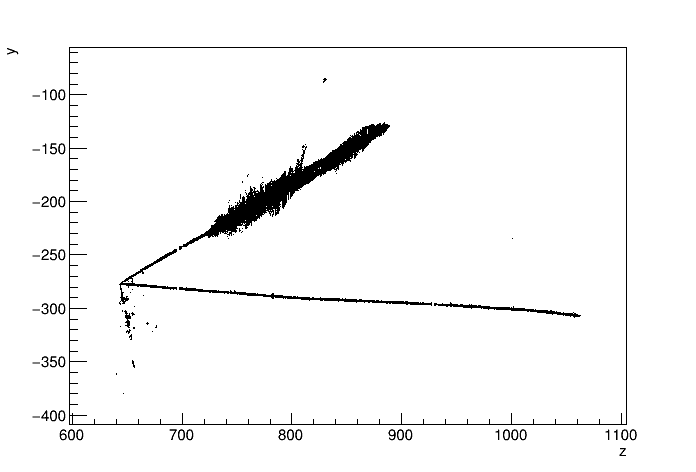
\includegraphics[width=.5\linewidth]{evd_zy_noreg_2302}\\
\makebox[.5\linewidth][c]{(a) All coincidences}
\makebox[.5\linewidth][c]{(b) Without regularization}\\
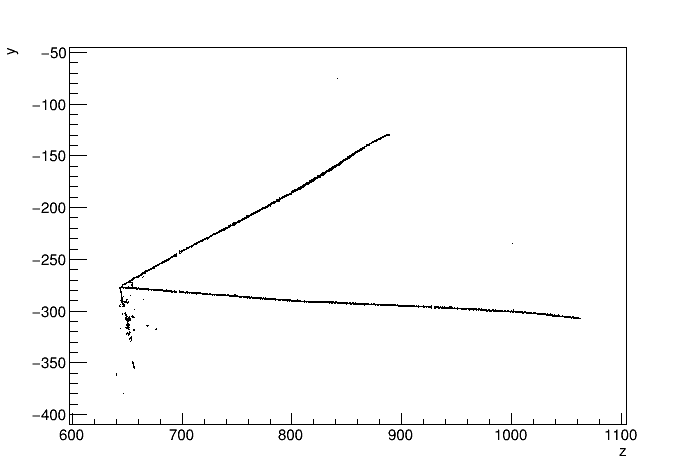
\includegraphics[width=.5\linewidth]{evd_zy_2302}
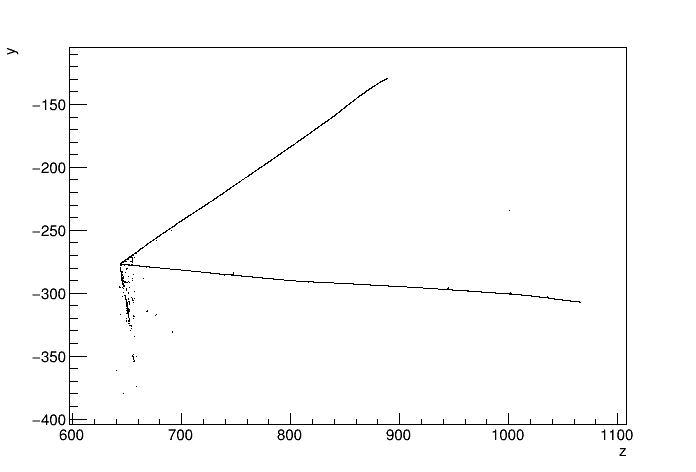
\includegraphics[width=.5\linewidth]{evd_zy_true_2302}
\makebox[.5\linewidth][c]{(c) With regularization}
\makebox[.5\linewidth][c]{(d) True charge distribution}\\

\caption[Event displays of SpacePointSolver performance]{Performance of SpacePointSolver on a simulated \dword{fd} neutrino interaction. The first panel shows the position of all triplet coincidences in the $zy$ view (looking from the side of the detector), displaying multiple ambiguous regions. The second and third panels show the solution with and without regularization, the regularization disfavouring various erroneous scattered hits. The final panel shows the true charge distribution, demonstrating %that 
the fidelity of the regularized reconstruction.}

\label{fig:spacepoint}
\end{figure}

The SpacePointSolver algorithm aims to transform the three \twod views provided by the wire planes into a single collection of \threed ``space points.''

First, triplets of wires are found with hits that are coincident in time within a small window (corresponding to \SI{2}{mm} in the drift direction) and where the crossing positions of the wires are consistent within \SI{3.55}{mm}. In some cases a collection wire hit may have only a single candidate pair of induction hits and the space point can be formed immediately. Often though, there are multiple candidate triplets, for example when two tracks are overlapped as seen in one view.

SpacePointSolver resolves these ambiguities by distributing the charge from each collection wire hit between the candidate space points so as to minimize the deviations between the expected and observed charges of the induction wire hits

\begin{equation}
\chi^2 = \sum_i^{\rm wires} \left(q_i - \sum_j^{\rm points}T_{ij}p_j\right)^2
\end{equation}

where $q_i$ is the charge observed in the $i^{\rm th}$ induction hit, $p_j$ is the solved charge at space point $j$, and $T_{ij}\in\{0,1\}$ encodes whether space point $j$ is coincident in space and time with wire hit $i$.

The minimization is subject to the condition that each predicted charge $p_j\ge0$, and that the total predicted charge for each collection wire hit exactly matches observations:

\begin{equation}
\sum_j^{\rm points}U_{jk}p_j=Q_k
\end{equation}

where $Q_k$ is the charge observed on the $k^{\rm th}$ collection wire, and $U_{jk}$ encodes the coincides of space point charges with the collection wires.

The problem as formulated is convex and can thus be solved exactly in a deterministic fashion. A single extra term can be added to the expression while retaining this property:

\begin{equation}
\chi^2 \to \chi^2 - \sum_{ij}^{\rm points}V_{ij}p_ip_j .
\end{equation}

By setting $V_{ij}$ larger for neighboring points this term acts as a regularization such that solutions with a denser collection of space points are preferred. The $V$ function is chosen empirically to have an exponential fall-off with constant \SI{2}{cm}.
%The algorithm is described more completely in \cite{spacepoint}.

Figure \ref{fig:spacepoint} shows the performance of this algorithm on a sample \dword{fd} \dword{mc} event, demonstrating good performance at eliminating spurious coincidences, and the importance of the regularization term.

SpacePointSolver was developed with the intention of acting as the first stage of a fully \threed reconstruction for \dword{fd} neutrinos, but it has been successfully put to use in a more restricted role to solve the disambiguation problem in \dword{protodune}. The full problem is solved, but for this application the information retained is restricted to the drift volume to which the corresponding space points for each induction hit are assigned. This technique correctly resolves more than 99\% of hits while requiring less CPU time than the standard disambiguation algorithm.

\subsubsection{Disambiguation}
The induction wires are wrapped in the \dword{fd} TPC design in order to save cost on electronics and minimize dead region between \dword{apa}s. The consequence is that multiple induction wire segments will be read out by the same electronic channel. We need to determine which wire segment corresponds to the energy deposited by the particle in the TPC. This process is called disambiguation. 

The \dword{fd} disambiguation algorithm was originally developed for the \dword{35t} geometry. It relies on the fact that the collection wires are not wrapped and the wire angles are slightly different for the two inductions views (44.3$^{\circ}$ versus 45.7$^{\circ}$) in the \dword{35t} so that any three wires from the three planes read out by the same three channels will never cross twice. The algorithm uses gaushit as input. All the collection hits are unambiguous. Each induction hit has one channel ID and several possible wire IDs corresponding to various wire segments read out by the same channel. We need to determine the correct wire ID % which wire ID is the correct one 
for each induction hit. The disambiguation algorithm first loops over all collection hits. For each collection hit, it loops over all induction hits and looks for one hit on each of the two induction planes that are in time with the collection hit. Once the triplet of hits is found (one on each plane with a common time), the algorithm checks all possible wire IDs and looks for three wires that intersect. Once one and only one intersection is identified, the two induction wire IDs are assigned to the two induction hits and the ambiguation is resolved. Finally the algorithm loops over all unresolved induction hits. For each hit, it loops over all possible wire segments for that channel and chooses the wire segment that is closest to a resolved induction hit as the correct wire segment. 

The \dword{protodune} disambiguation algorithm uses the outcome of the SpacePointSolver reconstruction, which associate a \threed point with three hits on three wire planes. The \threed point can be projected onto the induction plane and the ambiguity of the induction wire signal can be resolved by choosing the wire segment that is closest to the \threed point projection. 
%(RS: protoDUNE's APAs should see signals from single TPC only)

%\subsection{Blurred Cluster}\label{sec:BlurredCluster}
%The Blurred Cluster reconstruction method aims to construct two-dimensional shower-like clusters from deposits left in the detector by showers.  It specialises in shower reconstruction, especially in the separation of nearby showers in the reconstruction of, e.g., $\pi^0$ decay.  The algorithm first applies a weighted \twod Gaussian smearing to the hit map in order to introduce `fake hits' and distribute the charge deposited in the detector more realistically.  This proceeds by convolution of a Gaussian kernel, uniquely applied for each hit given information such as rough directionality of the showering particles and the width of the reconstructed hits in time in order to introduce the most accurate blurring possible.  Clustering follows by grouping neighbouring hits within the blurred region before removing any artificial hits and forming output clusters from the remaining hit collections.  BlurredCluster uses disambiguated gaushit as input and the output clusters are in turn used as input to the EMShower algorithm (see Section \ref{sec:EMShower}).  More details and detailed discussion are available in Ref~\cite{ref:blurredcluster}.

\subsection{Hit Clustering, and Track and Shower Reconstruction}

\subsubsection{Line Cluster}\label{sec:LineCluster}
The intent of the Line Cluster algorithm is to construct \twod line-like clusters using local information. The algorithm was originally known as Cluster Crawler. The ``Crawler'' name is derived from the similarity of this technique to ``gliders'' in \twod cellular automata. The concept is to construct a short line-like ``seed'' cluster of proximate hits in an area of low hit density where hit proximity is a good indication that the hits are indeed associated with each other. Additional nearby hits are attached to the leading edge of the cluster if they are similar to the hits already attached to it. The conditions are that the impact parameter between a prospective hit and the cluster projection is similar to those previously added and the hit charge is similar as well. These conditions are moderated to include high charge hits that are produced by large $dE/dx$ fluctuations and the rapid increase in $dE/dx$ at the end of stopping tracks while rejecting large charge hits from $\delta$-rays.
Seed clusters are formed at one end of the hit collection so that crawling in only one direction is sufficient. LineCluster uses disambiguated gaushits as input and produces a new set of refined hits. More details on the Line Cluster algorithm can be found in~\cite{ref:linecluster}.

\subsubsection{TrajCluster}\label{sec:TrajCluster}
TrajCluster reconstructs \twod trajectories in each plane. It incorporates elements of pattern recognition and Kalman Filter fitting. The concept is to construct a short ``seed'' trajectory of nearby hits. Additional nearby hits are attached to the leading edge of the trajectory if they are similar to the hits already attached to it. The similarity requirements use the impact parameter between the projected trajectory position and the prospective hit, the hit width and the hit charge. This process continues until a stopping condition is met such as lack of hits, an abnormally high or low charge environment, or encountering a \twod vertex or a Bragg peak.

\twod vertices are found between trajectories in each plane. The set of \twod vertices is matched between planes to create \threed vertices. A search is made of the ``incomplete'' \threed vertices, those that are only matched in two planes, to identify trajectories in the third plane that were poorly reconstructed.

Two recent additions to TrajCluster are matching trajectories in \threed and tagging of shower-like trajectories. More details on the TrajCluster algorithm can be found in~\cite{ref:trajcluster}.



\subsubsection{Pandora}\label{sec:Pandora}

The \dword{pandora} software development kit~\cite{Marshall:2015rfa} was created to address the problem of identifying energy deposits from individual particles in fine-granularity detectors, using a multi-algorithm approach to solving pattern-recognition problems. Complex and varied topologies in particle interactions, especially with the level of detail provided by \lartpc{}s, are unlikely to be solved successfully by a single clustering algorithm. Instead, the \dword{pandora} approach is to break the pattern recognition into a large number of decoupled algorithms, where each algorithm addresses a specific task or targets a particular topology. The overall event is then built up carefully using a chain of many tens of algorithms. The \dword{pandora} multi-algorithm approach has already been applied to \lartpc{} detectors, and has been successfully used in different analyses for the automated reconstruction of cosmic ray muons and neutrino interactions in the MicroBooNE experiment~\cite{Acciarri:2017hat} as well as test beam interactions in the \dword{pdsp} detector (see Section~\ref{sec:Pandora:ProtoDUNE}).


%\subsubsection{Pandora Inputs and Outputs}

%The sole input to the Pandora pattern recognition is a list of reconstructed and disambiguated 2D Hits, along with detector information (such as dimensions, unresponsive or dead material regions, etc.). Via the {\it larpandora} repository, which integrates Pandora pattern recognition algorithms into the LArSoft framework, these hits are translated into native Pandora 2D hits and separated into the different views and into ``drift volumes'', defined as the regions of the detector with a common drift readout. The specified chain of pattern recognition algorithms is then initialised and applied. 

%The results of the pattern recognition are output into the ART/LArSoft framework, again via {\it larpandora}. The output of the reconstruction is illustrated in Figure~\ref{larsoft_output}, being the main output a list of reconstructed 3D particles (termed ``PFParticles'', where ``PF'' stands for Particle Flow) for each event. A PFParticle corresponds to a distinct track or shower in the event, and has associated collections (Clusters) of 2D hits for each view, as well as an associated set of reconstructed 3D positions (SpacePoints) and a reconstructed Vertex position that defines its interaction point or first energy deposit. Navigation along PFParticle hierarchies is achieved using the PFParticle interface, which connects parent and daughter PFParticles, providing the Particle Flow describing the interaction. In the reconstruction of neutrino interactions, a neutrino PFParticle is also created and forms the top-level parent particle in each reconstructed neutrino hierarchy, with only a Vertex associated to it. Pandora also provides a second level of ART associations linking elements such as Clusters, Slices, SpacePoints, Tracks and Showers with their corresponding collection of Hits. 

%Pandora uses the concept of {\it slice} internally to represent and separate subsets of hits topological distinct, based on distance and pointing information, with the aim of avoiding merging together into one hierarchy particles produced by the interaction of a neutrino or test beam particle and those with cosmic ray origin. An ART/LArSoft product is now also available to identify PFParticles and Hits that belong to the same {\it slice}. For PFParticles, this information is also stored in the Metadata object, which contains as well information handled internally by Pandora that might be helpful for usage downstream, namely whether a particle was identified as a clear cosmic, or the scores of the multivariate analysis tools, such as Boosted Decision Trees (BDTs) or Support Vector Machines (SVMs) that were used to identify the test team particle or the neutrino interaction respectively. 

%The identity of each particle is currently not reconstructed by Pandora, but PFParticles are instead characterised as track-like or shower-like using the topological information available at this stage, according to the pattern of their hits. Then, for each PFParticle a higher level object will be created, either a Track or a Shower depending on its classification, containing extra information such as direction, opening angle, etc.  

%\begin{figure}[!h!tbp]
%\centering
%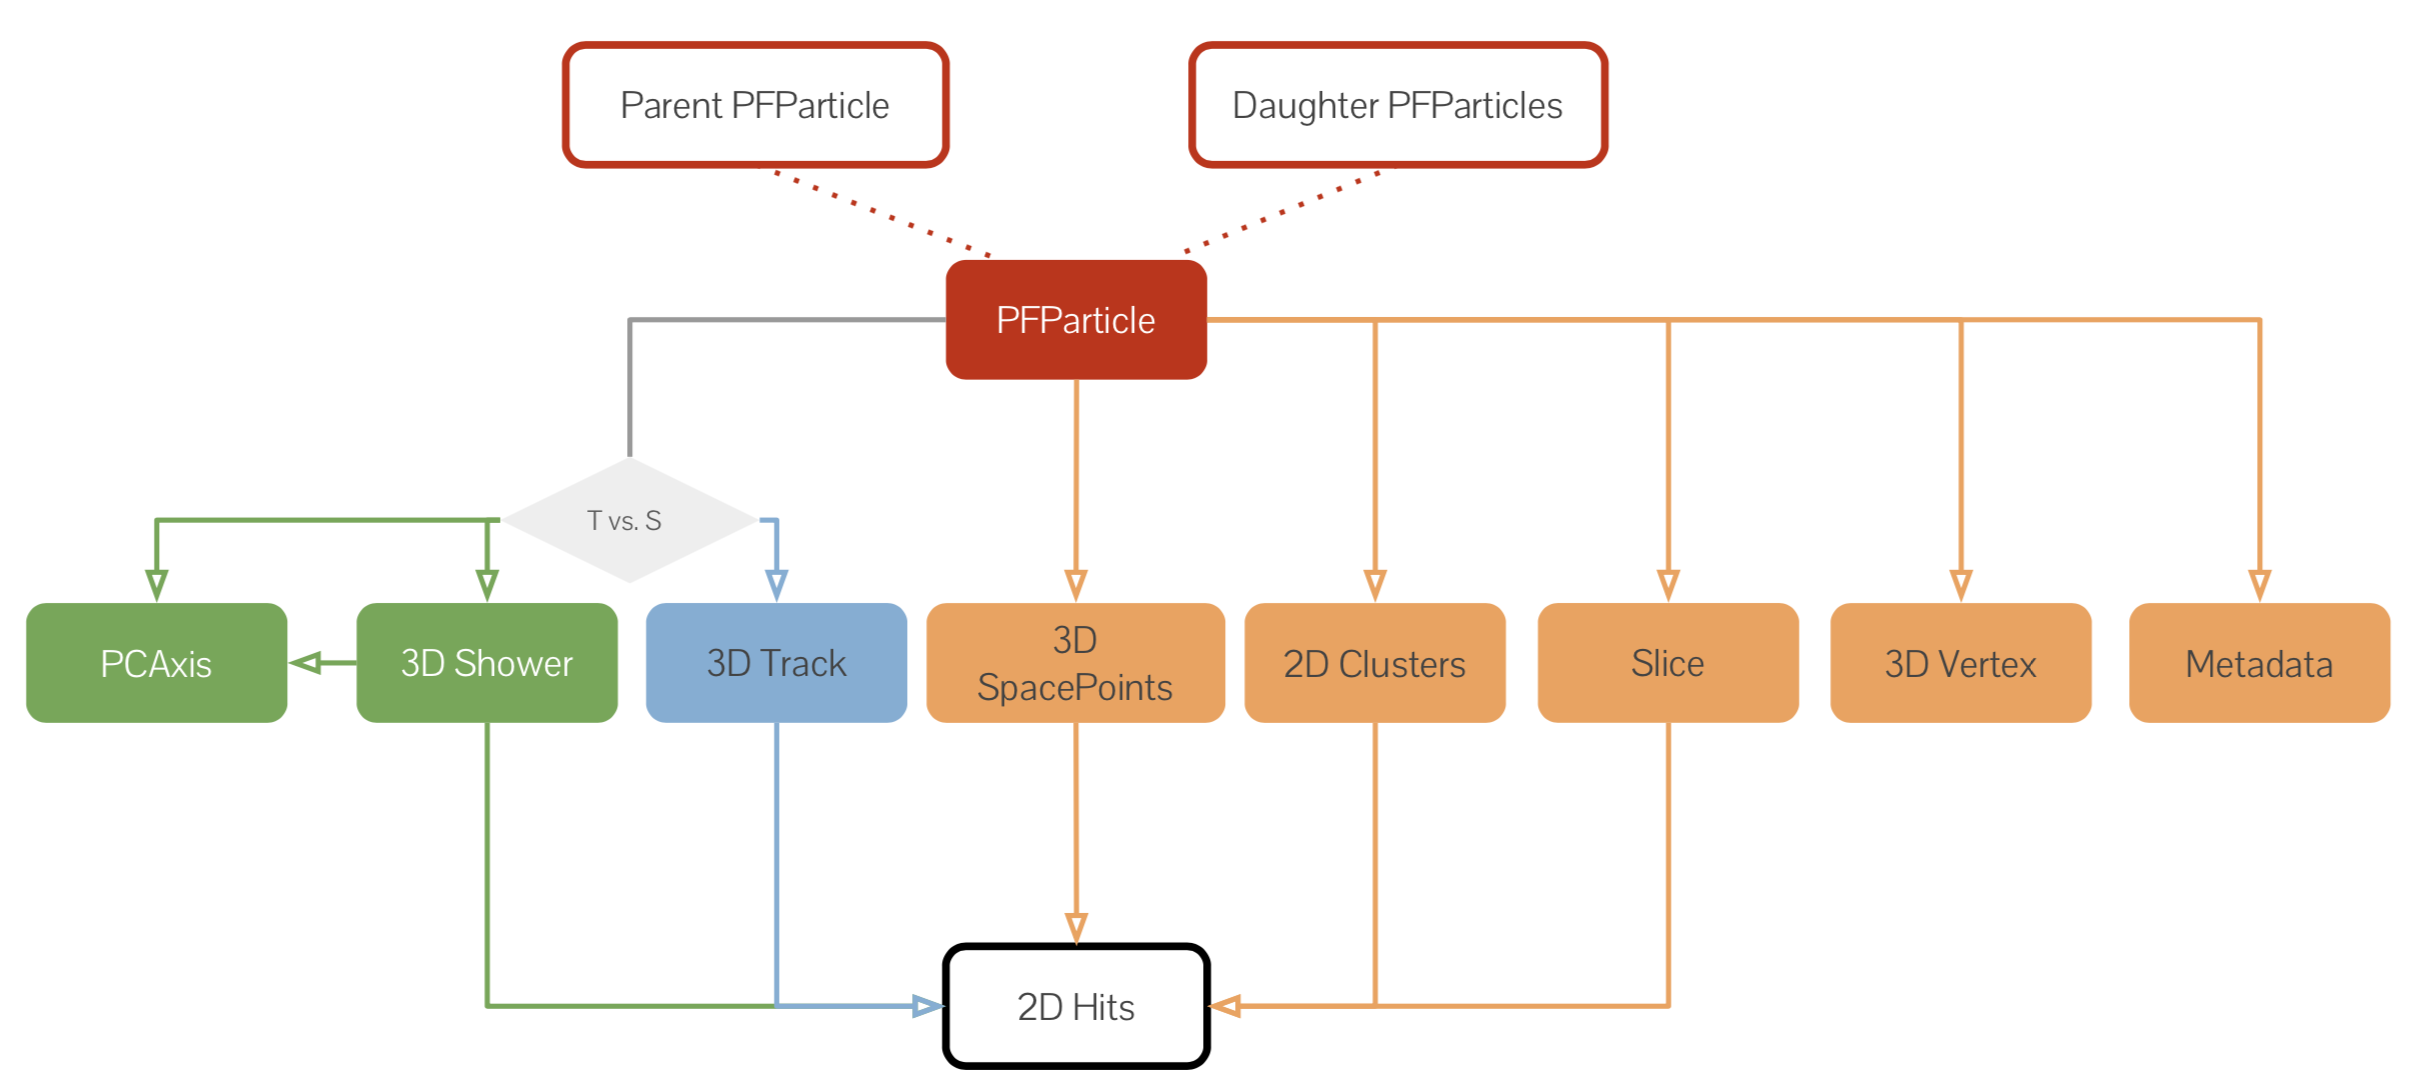
\includegraphics[width=0.8\textwidth]{./FIG_LArPandoraOutputNew.png}
%\caption{Illustration of the Pandora output in ART/LArSoft. Navigation along PFParticle hierarchies is achieved using the PFParticle interface, represented by dashed lines. Navigation from PFParticles to their associated objects is represented by solid arrows, as well as the second level of ART associations from these objects to the underlying Hits input to Pandora.}
%\label{larsoft_output}
%\end{figure}

%\subsubsection{Overview of the Pandora Pattern Recognition Algorithms}

The input to the \dword{pandora} pattern recognition is a list of reconstructed and disambiguated \twod hits, alongside detector information (such as dimensions, unresponsive or dead material regions). On these input hits (once translated into native \dword{pandora} \twod hits), the specified chain of pattern-recognition algorithms is applied. The results of the pattern recognition are persisted in the \dword{art}/\dword{larsoft} framework, with the major output being a list of reconstructed \threed particles (termed ``PFParticles'', where ``PF'' stands for particle flow). A PFParticle corresponds to a distinct track or shower in the event, and has associated objects such as collections of \twod hits for each view (Clusters), \threed positions (SpacePoints) and a reconstructed Vertex position that defines its interaction point or first energy deposit. Navigation along PFParticle hierarchies is achieved using the PFParticle interface, which connects parent and daughter PFParticles, providing a Particle Flow description of the interaction. The identity of each particle is currently not reconstructed by \dword{pandora}, but PFParticles are instead characterized as track-like or shower-like based on their topological features. 

The main stages of the \dword{pandora} pattern recognition chain are outlined below, and illustrated in Figure~\ref{reco_steps}. Note that both the individual pattern recognition algorithms and the overall reconstruction strategy are under continual development and will evolve over time, with a current emphasis %being the 
on the inclusion of machine-learning approaches to drive decisions in some key algorithms. The current chain of pattern-recognition algorithms has largely been tuned for neutrino interactions from the \fnal Booster Neutrino Beam; however, the algorithms are designed to be generic and easily reusable, and they are in the process of being adapted for neutrino interactions in the energy regime of DUNE. A more detailed description of the algorithms can be found in~\cite{Acciarri:2017hat}. 


\begin{enumerate}
\item{\bf Input hits:} The input list of reconstructed and disambiguated \twod hits are translated into native \dword{pandora} \twod hits and separated into the different views and into ``drift volumes'', defined as the regions of the detector with a common drift readout.
\item{\bf \twod track-like clusters:}  The first phase of the \dword{pandora} pattern recognition is track-oriented \twod clustering, creating ``proto-clusters'' that represent continuous, unambiguous lines of \twod hits. This early clustering phase is careful to ensure that the proto-clusters have high purity (i.e., represent energy deposits from exactly one true particle) even if this means they are initially of low completeness (i.e., only contain a small fraction of the total hits within a single true particle). A series of cluster-merging and cluster-splitting algorithms then examine the \twod proto-clusters and try to extend them, making decisions based on topological information, aiming to improve completeness without compromising purity.
\item{\bf \threed vertex reconstruction:} The neutrino interaction vertex is an important feature point. Once identified, any \twod clusters can be split at the projected vertex position, reducing chances of merging particles in any view. Cluster-merging operations also take proximity to the vertex into account, in order to protect primary particles emerging from the vertex region, and ensure good reconstruction performance for interactions with many final-state particles. Pairs of \twod clusters from different views are first used to produce lists of possible \threed vertex positions. These candidate vertices are examined and scored, and the best vertex is selected. \dword{pandora} has developed different algorithms for the selection of the neutrino vertex, including the use of machine-learning approaches in MicroBooNE. Similar approaches can be harnessed in the future for interactions in %DUNE FD
the \dword{fd}, where a score-based approach is currently used.
\item{\bf \threed track reconstruction:} The aim of the \threed track reconstruction is to identify the combinations of \twod clusters (from the different views) that represent the same true, track-like particle. These \twod clusters are formally associated by the construction of a \threed track particle. During this process, \threed information can also be used to improve the quality of the \twod clustering. A \dword{pandora} algorithm considers all possible combinations of \twod clusters, one from each view, and builds (what is loosely termed) a rank-three tensor to store a comprehensive set of cluster-consistency information. This tensor can be queried to identify and understand any cluster-matching ambiguities. \threed track particles are first built for any unambiguous combinations of \twod clusters. Cases of cluster-matching ambiguities are then addressed, with iterative corrections to the \twod clustering being made to resolve the ambiguities and so enable \threed particle creation.
\item{\bf \twod and \threed shower reconstruction:} A series of topological metrics (additional use of some calorimetric information would be desirable in the future) are used to characterize each \twod cluster as track-like or shower-like. This information is analyzed to identify the longest shower-like clusters, which form the ``seeds'' or ``spines'' for \twod and \threed shower reconstruction. A recursive algorithm is used to add shower branches onto each top-level shower seed, then branches onto branches, etc. The \twod showers are then matched between views to form \threed showers, reusing ideas from the \threed track-matching procedure.
\item{\bf \twod and \threed particle refinement and event building:} Following the \threed track and shower reconstruction, a series of algorithms is used to improve the completeness of the reconstructed particles by merging together any nearby particles that are just fragments of the same true particle. Both \twod and \threed approaches are used, %with a typical approach being to 
where a typical approach uses combinations of \twod clusters (from different views) to identify features in \threed, or projecting \threed features into each of the \twod views. This is a powerful demonstration of the \dword{pandora} rotational coordinate transformation system, which allows seamless use of \twod and \threed information to drive pattern-recognition decisions. Finally, \threed space points are created for each \twod input hit, and the \threed particle trajectories are used to organize the reconstructed particles into a hierarchy. Final-state particles can be navigated via parent-daughter links, thus reconstructing their subsequent interactions or decays. For neutrino interactions, a top-level reconstructed neutrino particle is created; it represents the primary particle in the hierarchy linking together the daughter final-state particles and provides the information about the neutrino interaction vertex.

\end{enumerate}

\begin{figure}[!h!tbp]
\centering
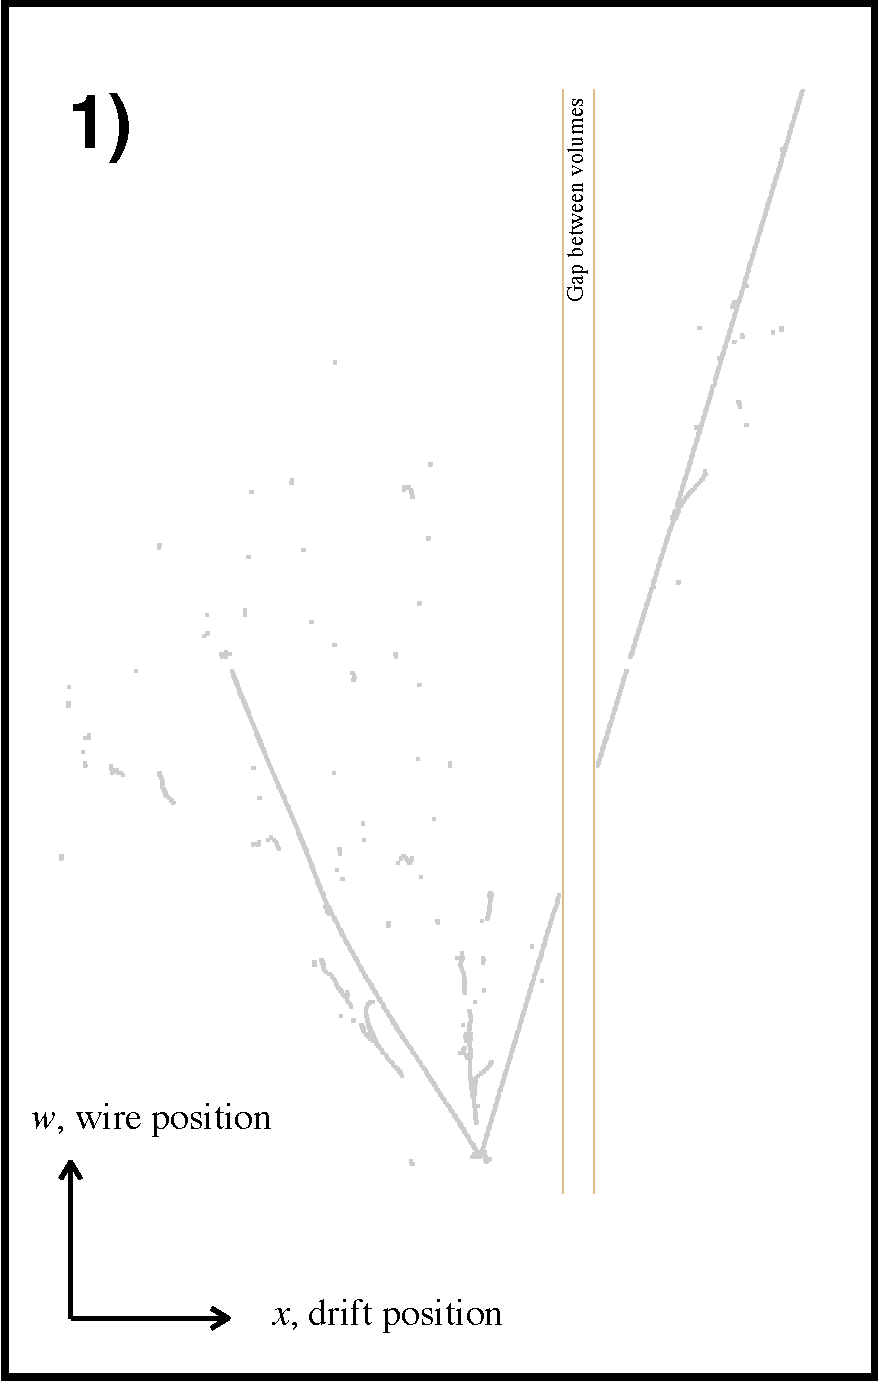
\includegraphics[width=5cm, height=7.5cm]{./Pandora/OneInputHits.pdf}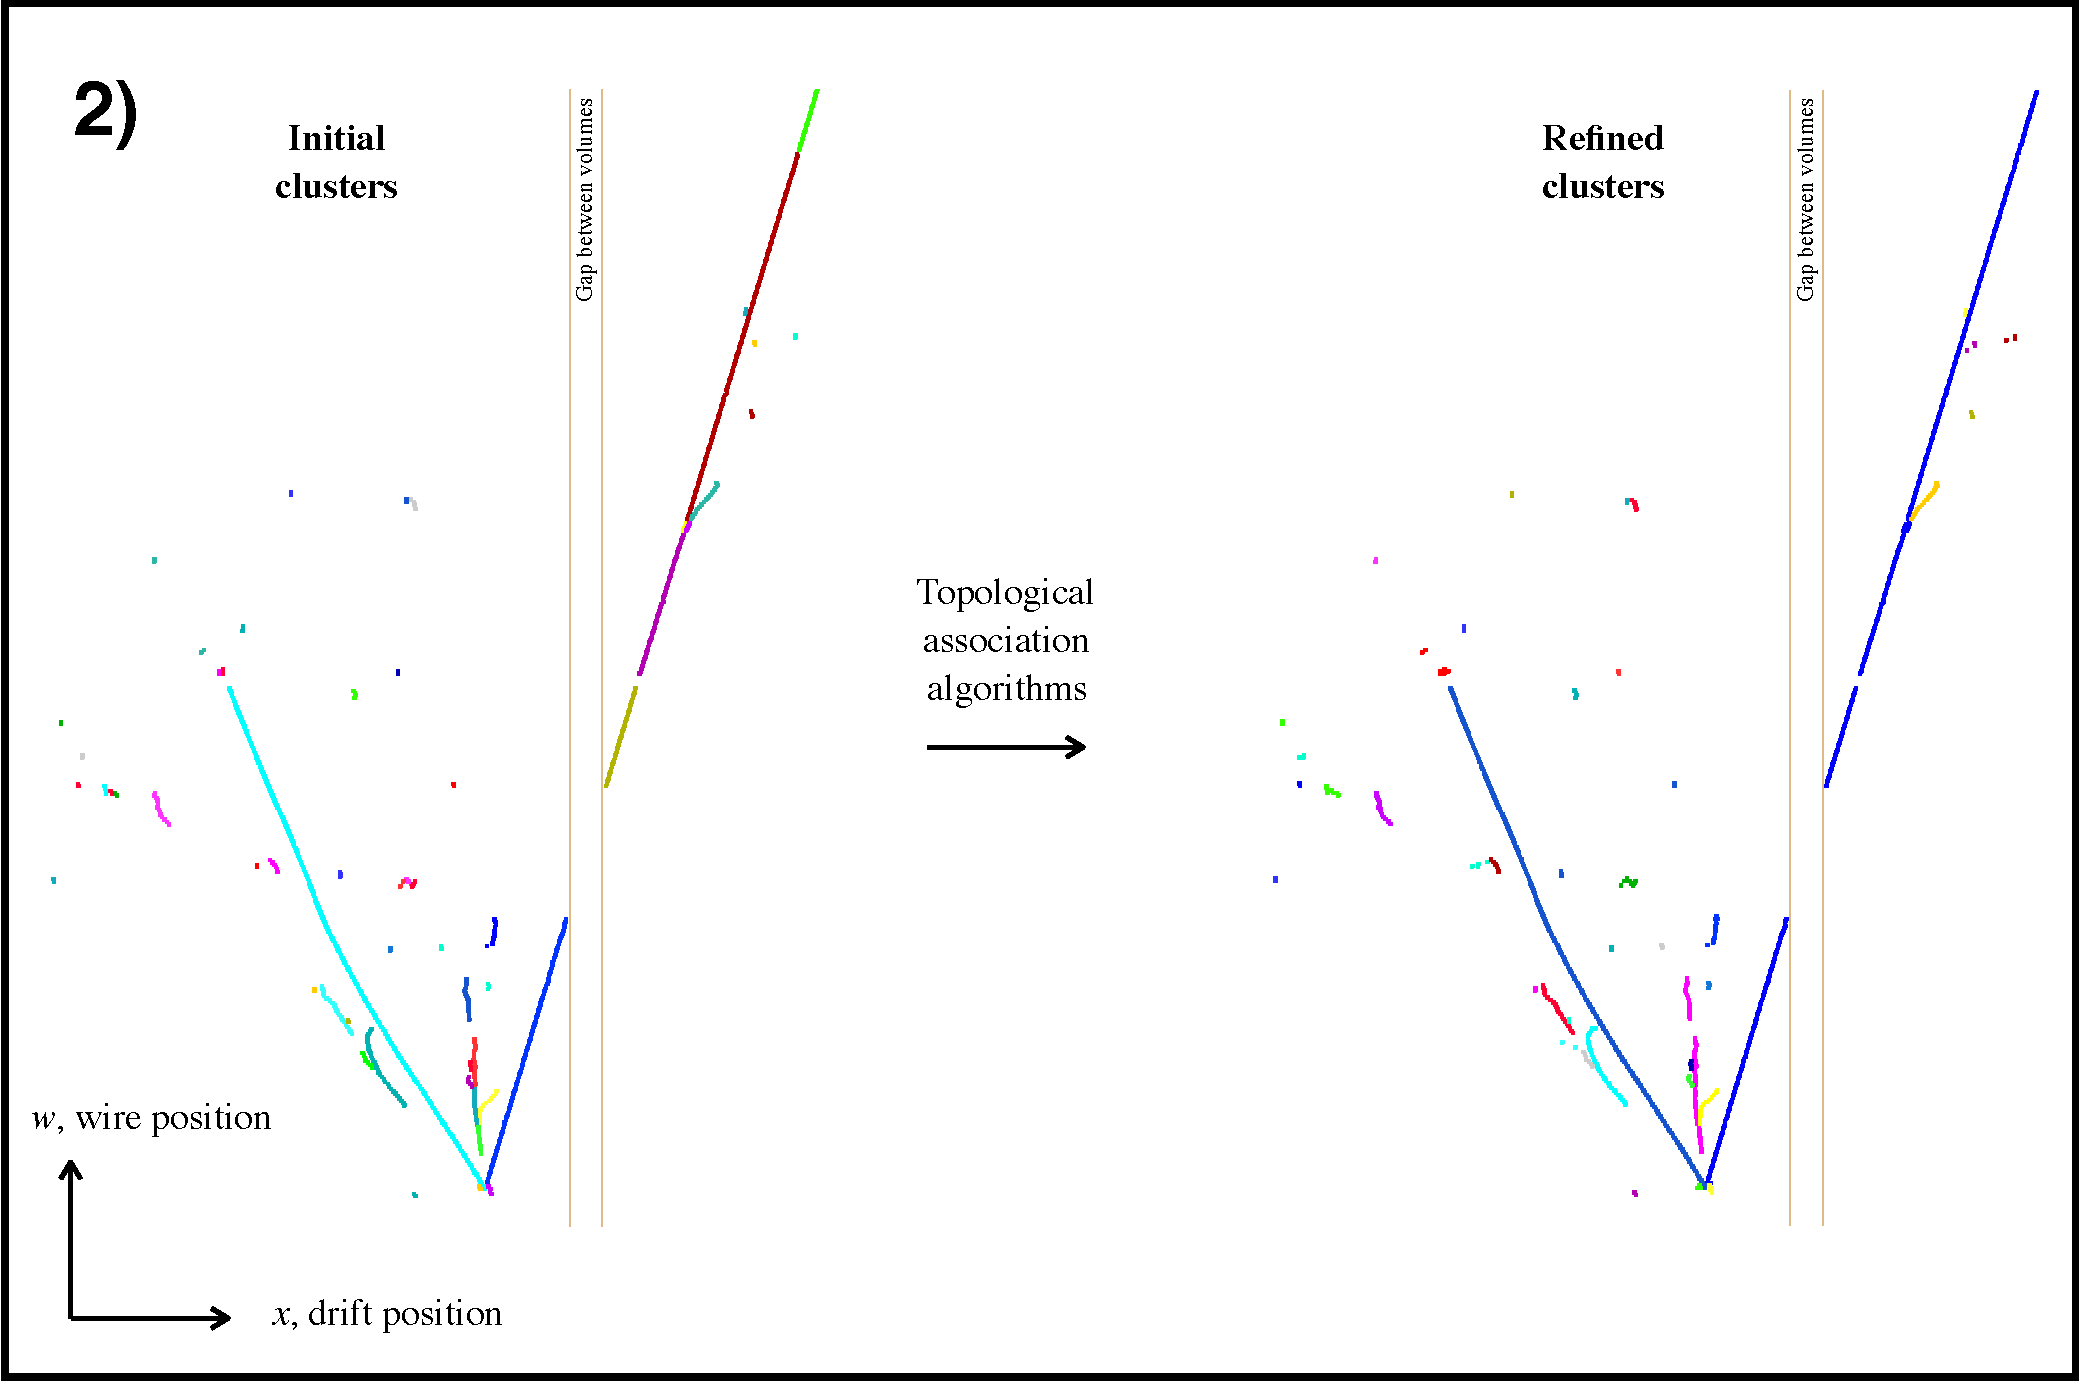
\includegraphics[width=13cm, height=7.5cm]{./Pandora/TwoPrePostTopAssoc.pdf}
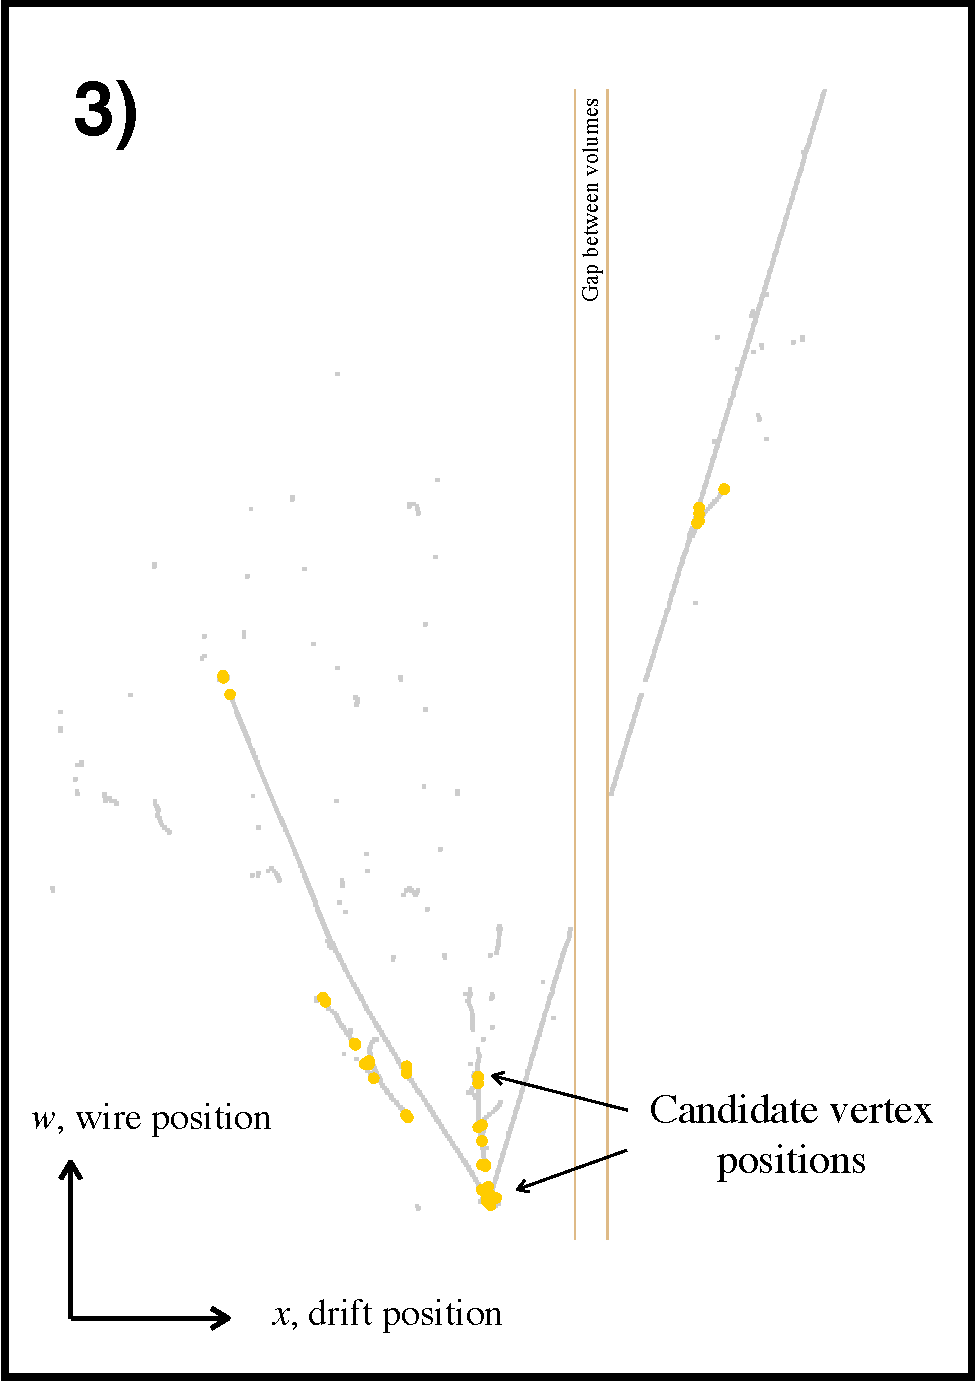
\includegraphics[width=5cm, height=7.5cm]{./Pandora/ThreeVertexCandidates.pdf}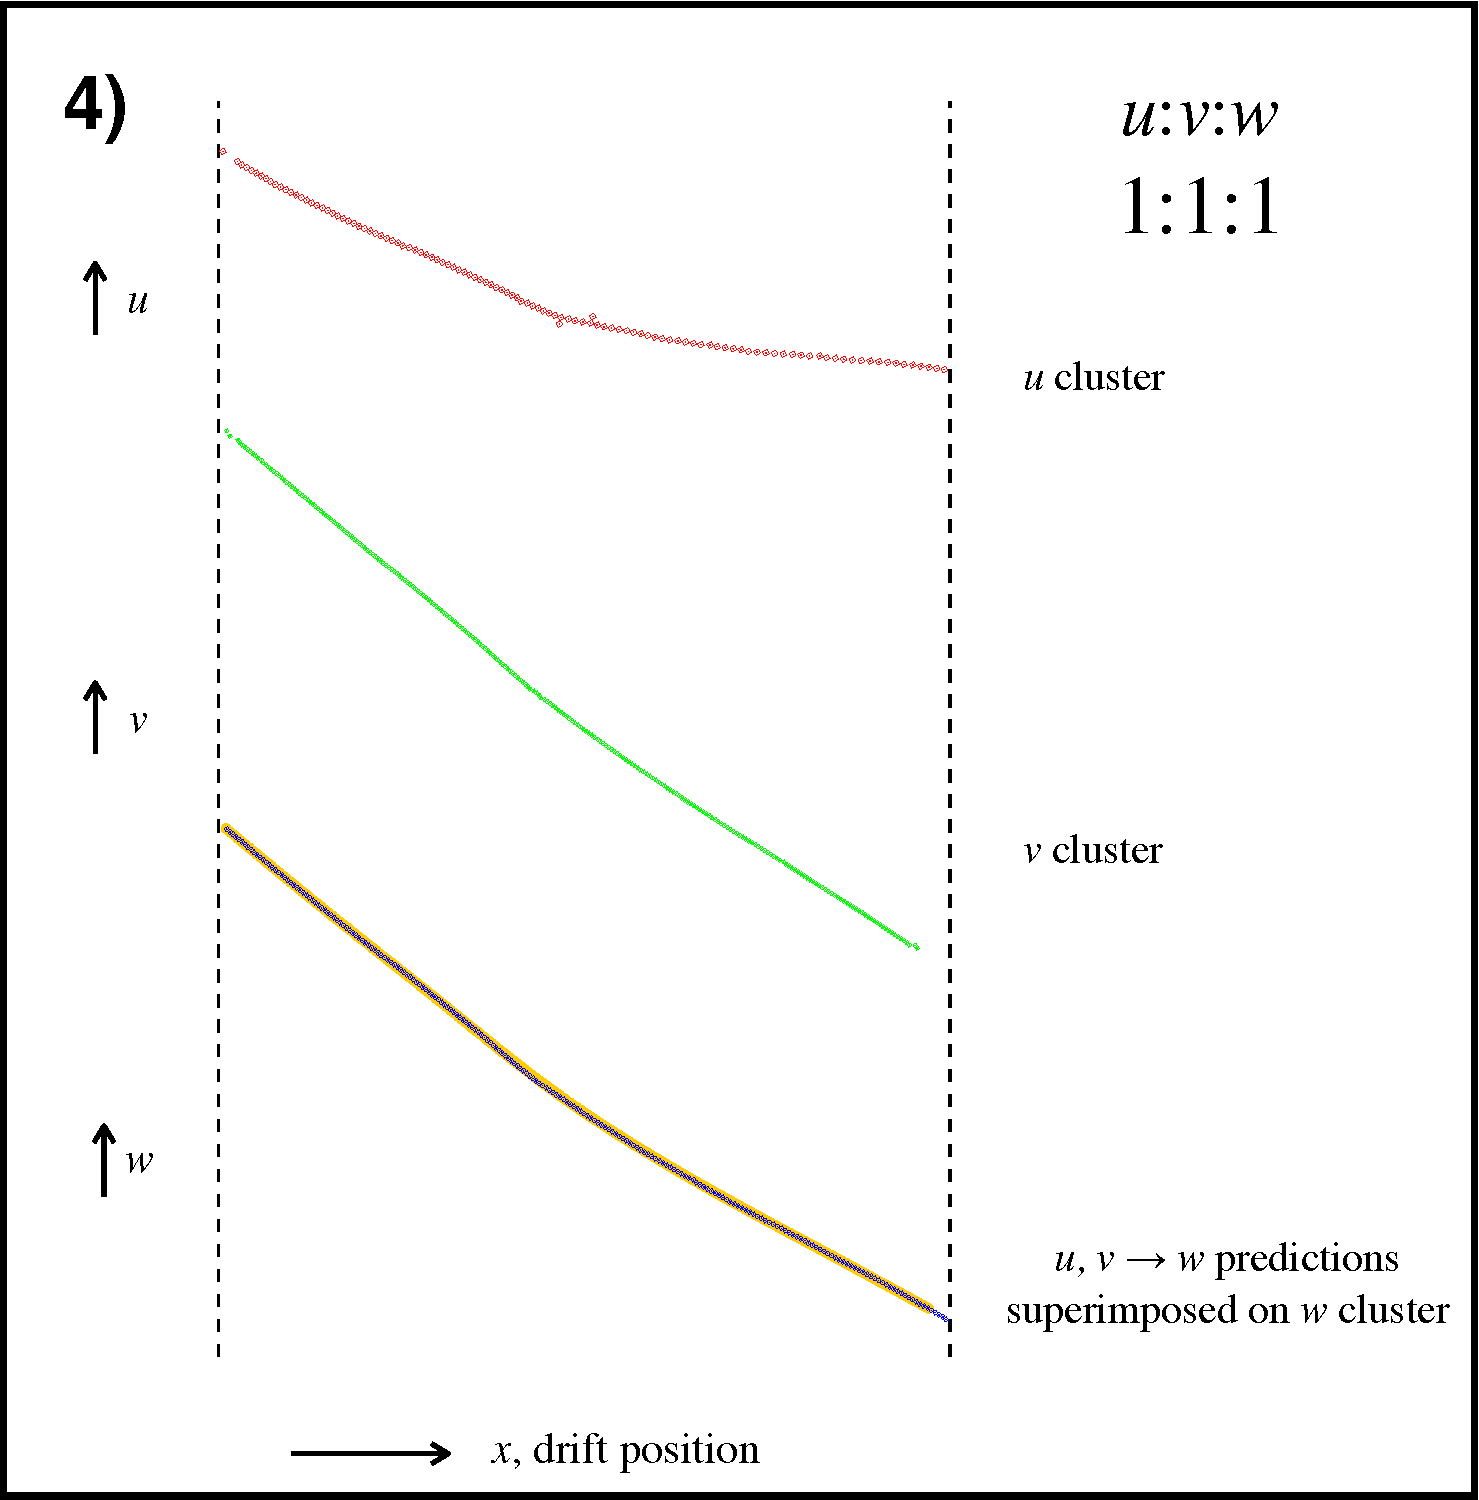
\includegraphics[width=7cm, height=7.5cm]{./Pandora/Four3DMatch.pdf}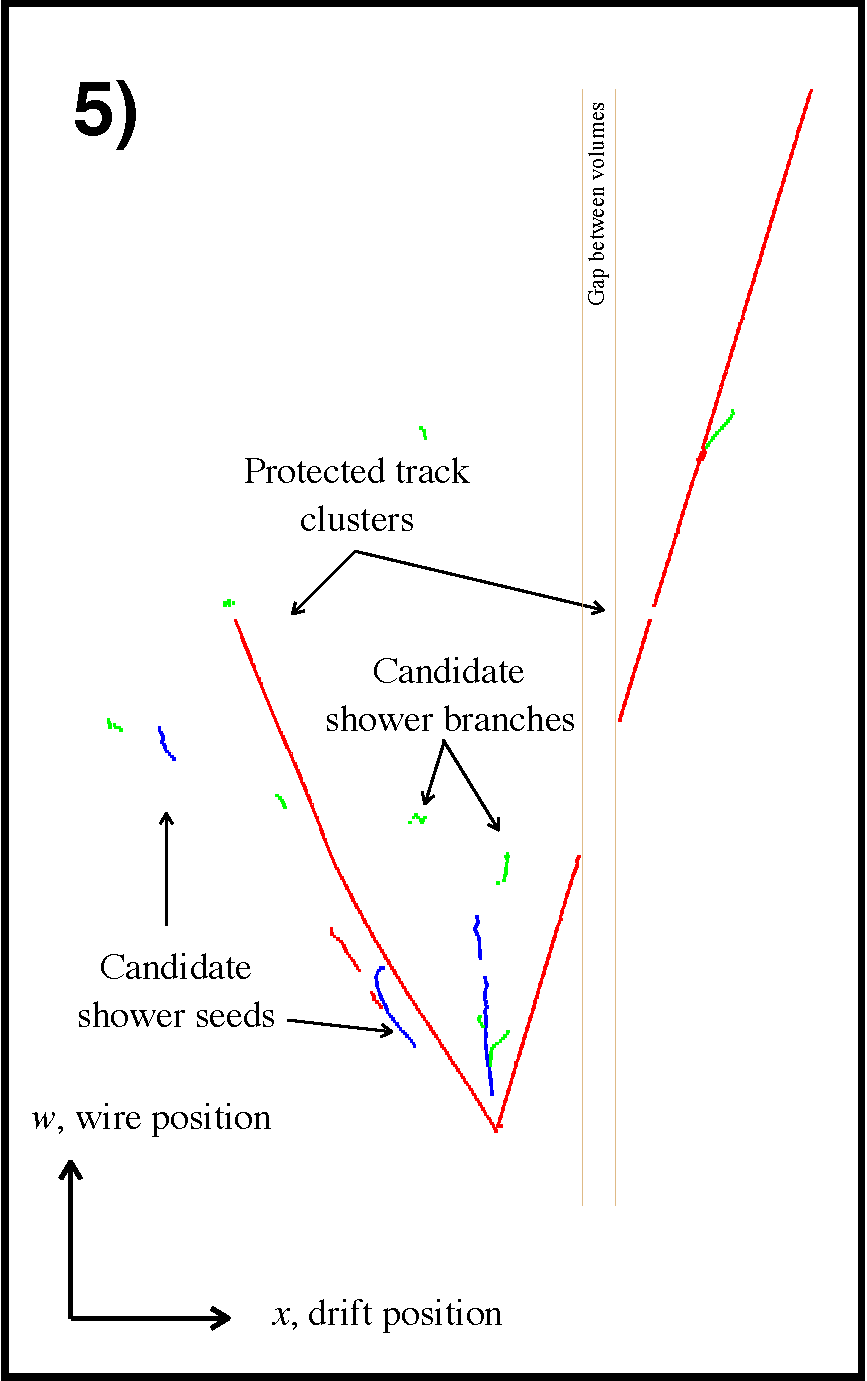
\includegraphics[width=6cm, height=7.5cm]{./Pandora/FiveTrackShower.pdf}
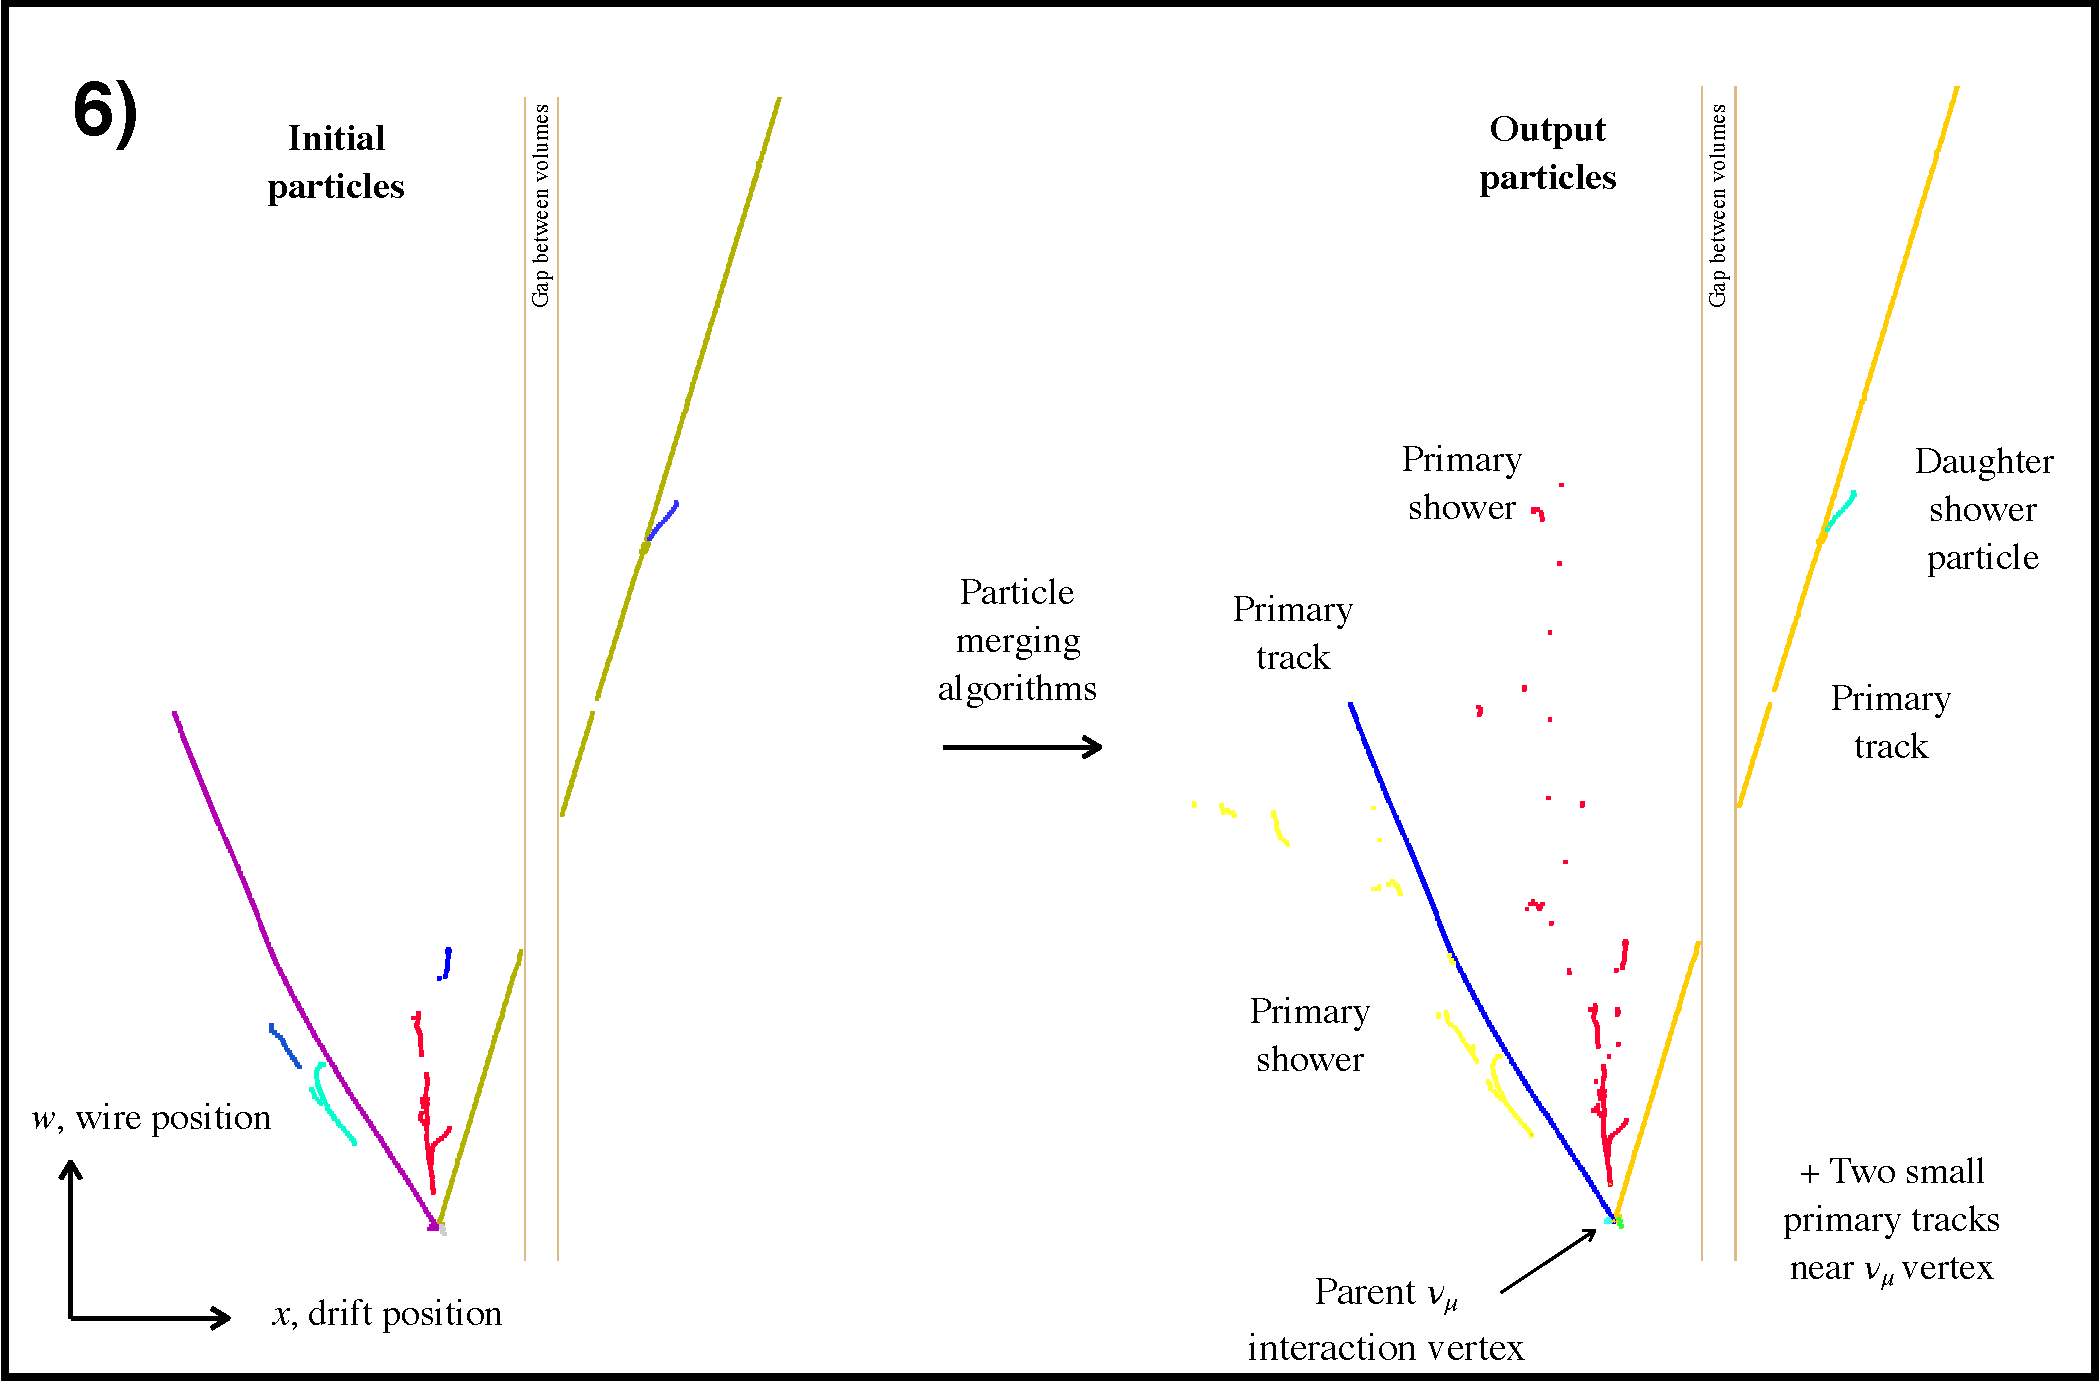
\includegraphics[width=12cm, height=7.5cm]{./Pandora/SixPrePostMopUp.pdf}
\caption{Illustration of the main stages of the \dword{pandora} pattern recognition chain: (1) Input Hits; (2) \twod track-like cluster creation and association; (3) \threed vertex reconstruction; (4) \threed track reconstruction; (5) Track/Shower separation; (6) \twod and \threed particle refinement and event building.}
\label{reco_steps}
\end{figure}

The algorithms forming the stages described above can be used in different ways, thanks to the multi-algorithm approach. Currently, two \dword{pandora} reconstruction paths ({\it PandoraCosmic} and {\it PandoraNu}) have been created, using chains of tens of algorithms each (note that over 130 algorithms and tools are used in total). Although many algorithms are shared between the two paths, the overall algorithm selection results in different key features:
\begin{enumerate}
\item PandoraCosmic: Strongly track-oriented, optimized for the reconstruction of cosmic-ray muons and their daughter (shower-like) delta rays. 
\item PandoraNu: Optimized for the reconstruction of neutrino or test beam particle interactions, carefully building the event using the reconstructed interaction vertex (protecting particles emerging from it) and including a careful treatment of tracks versus showers. 
\end{enumerate}

These two chains of algorithms are harnessed together to provide a consolidated output in the case of surface detectors exposed to cosmic rays, such as MicroBooNE and \dword{pdsp} (without significant cosmic-ray background, only the PandoraNu algorithm chain is necessary for the \dword{fd}). The overall reconstruction strategy in such detectors is illustrated in Figure~\ref{consolidated_reco}. It starts by running the PandoraCosmic reconstruction on the entire collection of input hits, then identifies ``clear'' cosmic rays. This identification uses a geometrical approach to tag through-going cosmic rays and examines the consistency of the cosmic rays with the $t_{0}$ appropriate to the neutrino beam spill. Clear cosmic rays are output already at this stage. For the remaining ambiguous hits, however, additional stages are required. A \textit{slicing} process is applied to the remaining hits, dividing them into smaller regions (slices) that represent separate, distinct interactions. Each slice is reconstructed using both the PandoraNu and PandoraCosmic reconstruction chains and the results are compared directly to identify whether the slice corresponds to a cosmic ray or a neutrino interaction (in the case of MicroBooNE) or test beam interaction (in the case of \dword{pdsp}). The consolidated event output is formed of three classes of reconstructed particles: (1) clear cosmic rays, (2) cosmic rays that are spatially and temporally consistent with being a neutrino interaction in the detector (remaining cosmic-rays) and (3) candidate neutrino or test beam interactions.

\begin{figure}[!h!tbp]
\centering
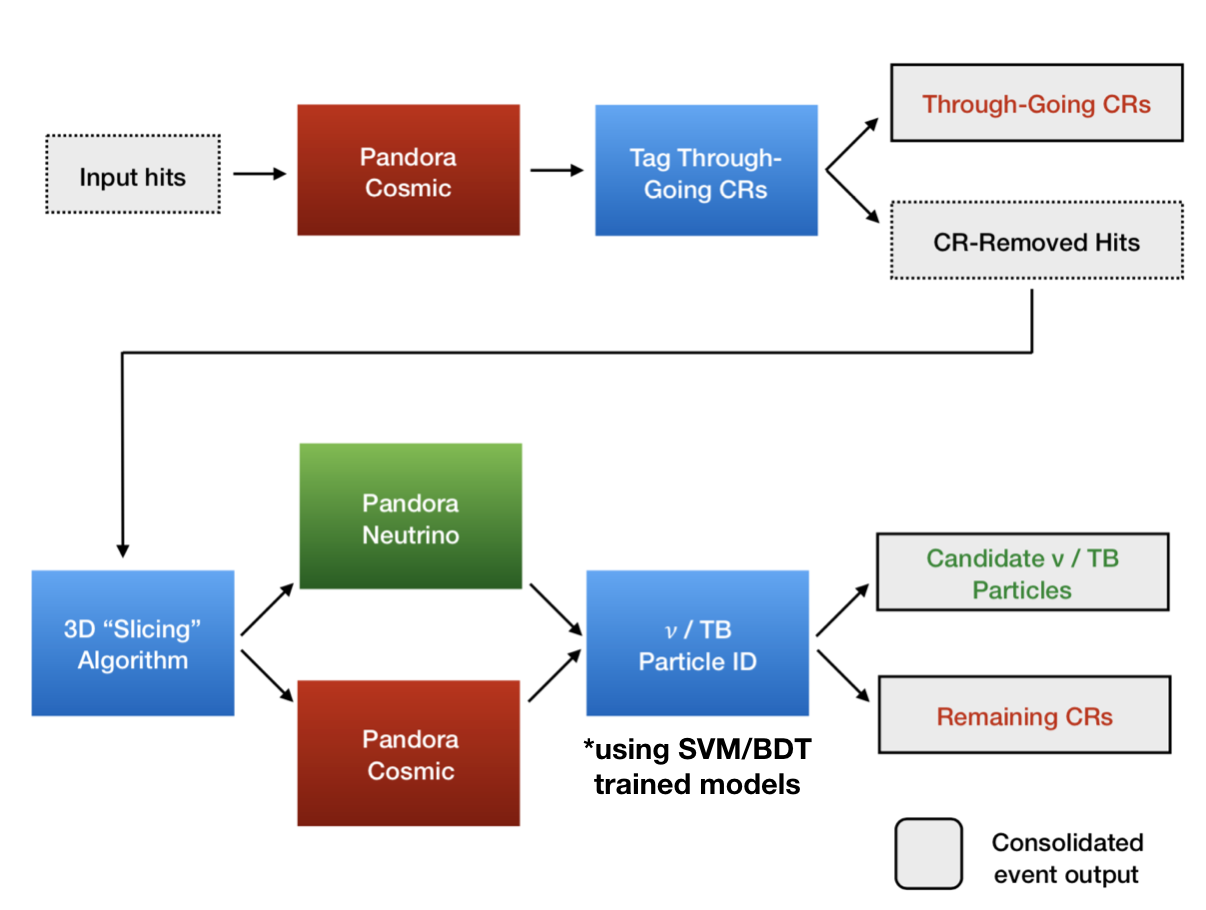
\includegraphics[width=0.65\textwidth]{./FIG_PandoraConsolidatedOutput.png}
\caption[Schema of the \dword{pandora} consolidated output and overall reconstruction strategy for surface LArTPCs]{Schema of the \dword{pandora} consolidated output and overall reconstruction strategy for surface LArTPCs such as MicroBooNE and \dword{pdsp}. See text for more details.}
\label{consolidated_reco}
\end{figure}

Of particular importance in this overall reconstruction strategy is the neutrino (MicroBooNE) or test beam particle (\dword{pdsp}) identification tool. This tool is responsible for deciding whether to output the cosmic ray or neutrino (or test beam) reconstruction outcomes for a given slice. For \dword{pdsp}, this decision is based on the output from adaptive \dwords{bdt}, trained to distinguish between cosmic-ray and test beam particles, which has proved to be highly efficient across the momentum range of \dword{pdsp} data (as it will be shown in Section ~\ref{sec:Pandora:ProtoDUNE}). %The variables used in this BDT model have proved to be highly efficient across the momentum range of ProtoDUNE-SP data (as it will be shown in Section ~\ref{sec:Pandora:ProtoDUNE}). These variables are: 

%\begin{itemize}
%\item The eigenvalues of the covariance matrix of the spatial position of the 3D LArTPC hits.
%\item The distance of the closest 3D hit to the beam spot.
%\item The vertical distance of the reconstructed 3D hit closest to the top of the detector.  
%\item The number of reconstructed particles.
%\item The angle and direction of a spatial fit to the reconstructed 3D hits with respect to the beam line.
%\end{itemize}

The performance obtained with the current algorithms are shown in Section~\ref{sec:performance}, both for the \dword{fd} and \dword{pdsp}.  As previously mentioned, both the individual pattern recognition algorithms and the overall reconstruction strategy are under continual development. Many algorithms %are still to be explicitly tuned 
still require explicit tuning for the DUNE energy ranges, and new algorithms, designed specifically for DUNE, will be added to the multi-algorithm pattern recognition. The performance presented in this document therefore represents a current snapshot and is expected to improve with future dedicated work. 


\subsubsection{Projection Matching Algorithm}\label{sec:PMA}
\dword{pma}  was primarily developed as a technique of \threed reconstruction of individual particle trajectories (trajectory fit) Ref~\cite{Antonello:2012hu}. \dword{pma} was designed to address a challenging issue of transformation from a set of independently reconstructed \twod projections of objects into a \threed representation. Reconstructed \threed objects are also providing  basic physics quantities like particle directions and $dE/dx$ evolution along the trajectories. \dword{pma} uses as its input the output from \twod pattern recognition: clusters of hits. For the purposes of the DUNE reconstruction chain the Line Cluster algorithm (Section~\ref{sec:LineCluster}) is used as input to \dword{pma}, however the use of hit clusters prepared with other algorithms may be configured as well. As a result of \twod pattern recognition, particles may be broken into several clusters of \twod projections, fractions of particles may be missing in individual projections, and clusters obtained from complementary projections % are not guaranteed to 
may not cover corresponding sections of trajectories. Such behavior is expected since ambiguous configurations of trajectories can be resolved only if the information from multiple \twod projections is used. Searching for the best matching combinations of clusters from all \twod projections was introduced to \dword{pma} implementation in the \dword{larsoft} framework. The algorithm also attempts to correct hit-to-cluster assignments using properties of \threed reconstructed objects. In this sense \dword{pma} is also a pattern-recognition algorithm.
The underlying idea of \dword{pma} is to build and optimize objects in \threed space (formed as polygonal lines with % an iteratively increased number of segments) 
the number of segments iteratively increased) by minimizing the cost function calculated simultaneously in all available \twod projections. %The cost function consists of the \twod distance of hits to the optimized object \twod projections, penalty of tracks curvature, and \threed distance of various feature points to the optimized object (used e.g., to improve performance for tracks with isochronous orientation).
%\fixme{please clarify prev sentence. anne} 
%The track can be reconstructed using clusters from two projections while the distance of hits to the track projection in the third plane is used to validate correct association of clusters. This method is used to score \threed track candidates in the three-plane TPC configurations, like the \dword{spmod}, %single-phase DUNE 
%MicroBooNE, %detectors 
%and prototypes. In this scenario clusters from all planes are used in the fine-tuning of the selected candidates. %In the two-plane configurations (\dual TPC detectors, \single LArIAT and ArgoNeut  detectors) the track candidates are scored by the value of the cost function, which is significantly increased if the trajectory fit is being optimized to spuriously associated clusters
 %\fixme{if we optimize the fit to do what with spuriously associated clusters? anne}(this is also a second-level criterion for the three-plane configurations %if 
 %in cases where the validation method shows no significant difference for track candidates).
%The approach of constructing entire objects in \threed %allows to avoid requirement of 
%avoids the need to find associations between \twod planes on the level of individual hits. Such associations are especially problematic if several hits on a single trajectory can be found with a similar drift time value, or, if  due to a low signal, for example, % (or any other reason) 
%hits are missed in one of projections. Unambiguous \threed position is calculated for each \twod hit, independently from other hits in the trajectory. Such \threed positions are more accurate than found with the ``standard'' calculation of a single \threed point using multiple \twod hits matched by drift time values, leading to the more accurate $dE/dx$ estimation. It also allows %to build 
%construction of \threed objects using the detector data from \twod planes directly, without an intermediate step of %a \threed points calculation which are subsequently 
%calculating \threed points for subsequent use in obtaining the final trajectory fit. Another advantage of the approach is the capability to estimate direction of small, few-hit tracks, %or estimation of 
%and to estimate the \threed PC axis of shower-like objects. \fixme{what's PC? anne}
Several features were developed in \dword{larsoft}'s \dword{pma} implementation to address detector-specific issues like stitching the particle fragments found in different TPCs or %an option for 
performing disambiguation at the \threed reconstruction stage. Since algorithms existing within or interfaced to the \dword{larsoft} framework (see Section \ref{sec:Pandora}) can provide pattern reconstruction results that include the particle hierarchy description, the mode for applying \dword{pma} to calculate %solely the 
trajectory fits alone was developed. In this mode the collections of clusters forming particles are taken from the ``upstream'' algorithm and  hit-to-cluster associations remain unchanged. %are not changed.


%Recent developments of PMA are relying on the same principle ideas and allow to build and optimize complex structures of \threed objects, i.e. multiple particle trajectories interconnected with interaction vertices. With such approach it is possible to employ in the vertex position reconstruction the local information from several tracks simultaneously, leading also to an improved fit of each individual trajectory. The track-vertex structure is constructed after the individual trajectories are found and stitched across TPC's. Vertex candidates are found as regions of intersection of two or more tracks (including regions found beyond the track endpoints), with the threshold on the allowed region size. Tracks shorter than $nn$ cm are treated separately; they can be associated to vertex candidates found using long tracks in the first pass of the algorithm or used to create vertex candidates in the second pass. Candidates are scored by the number of intersecting tracks, and if this number is equal for two candidates the maximum angle between intersecting tracks is used select candidate and create a better defined vertex as first. The entire track-vertex structure with the newly created vertex is re-optimized using PMA principles in order to accommodate additional information in the trajectory fits. Since the new vertices may connect structures that already contain vertices, a set of rules for splitting and flipping tracks was developed to ensure that the resulting structure is always tree-like (i.e. does not contain loops). The resulting structure is described as a particle hierarchy using data products available in \dword{larsoft}.

%\fixme{orig of next pgraph is commented above; I started rewording but I can't parse enough of it unambiguously. anne}
%Recent \dword{pma} developments rely on the same principle and allow building and optimizing complex structures of \threed objects, e.g., multiple particle trajectories interconnected with interaction vertices. This makes it possible to use the local information from several tracks simultaneously in the vertex position reconstruction, which leads to an improved fit for each individual trajectory. 
%
%\dword{pma} constructs the track-vertex structure after it finds the individual trajectories and stitches them across TPCs. Vertex candidates are found as regions of intersection of two or more tracks (including regions found beyond the track endpoints), with the threshold on the allowed region size. 
%\fixme{what threshold? and fix nn cm below}
%Tracks shorter than $nn$ cm are treated separately; they can be associated to vertex candidates found using long tracks in the first pass of the algorithm or \fixme{}used to create vertex candidates in the second pass. Candidates are scored by the number of intersecting tracks, and if this number is equal for two candidates the maximum angle between intersecting tracks is used select candidate and create a better defined vertex as first. The entire track-vertex structure with the newly created vertex is re-optimized using \dword{pma} principles in order to accommodate additional information in the trajectory fits. Since the new vertices may connect structures that already contain vertices, a set of rules for splitting and flipping tracks was developed to ensure that the resulting structure is always tree-like (i.e., does not contain loops). The resulting structure is described as a particle hierarchy using data products available in \dword{larsoft}.


%Two important reconstruction features are currently under development in \dword{larsoft}'s \dword{pma} implementation. The first is the integration of \dword{pma} input with the recognition 
%\fixme{integration with the `recognition'? Does that mean to add recognition capability to PMA? anne} of shower-like \twod objects (e.g., electromagnetic showers, electron tracks) and track-like objects (e.g., hadron and muon tracks). Such recognition is a prerequisite of obtaining robust \threed tracking with \dword{pma}, since different fitting strategies should be applied to track and shower objects. The second %feature under development %is the detection of kinks and decay points missed at the \twod pattern recognition level. First attempts were made %with the search 
%made by searching for outliers in the distribution of angles in the trajectory fit. It was found that the dependence on the track orientation in a \twod projection needs to be taken into account. In addition, a potential integration with an algorithm based on \twod \dword{adc} image analysis will be explored.


%\subsection{EMShower}\label{sec:EMShower}

%mode is used when reconstructing neutrino events.The EMShower reconstruction algorithm aims to find final 3D showers and all associated properties.  It is intentionally high-level by design and relies heavily on previous reconstruction, specifically BlurredCluster (Section \ref{sec:BlurredCluster}) and PMA (Section \ref{sec:PMA}).  The reconstruction proceeds in two general steps: first, the shower objects, including all associated hits in each of the views, are found; second, the properties of these showers, such as start point, direction, energy and initial dE/dx, are determined by multiple pattern recognition and calorimetric reconstruction algorithms.

%The shower objects are created by simply matching the previously found, well-formed, shower-like clusters (provided by BlurredCluster) between the different views to form 3D objects with associated hits in each plane.  This is achieved by associating hits between the \twod shower-like clusters and 3D tracks (provided by, e.g., PMA) in order to pull together clusters from different planes into one object.  These shower hits are then analysed by various successive algorithms in order to find relevant properties before the output shower objects are constructed for later use.

%EMShower can be configured to use hits from the shower-like PFParticles identified by the Pandora package. This mode is used when reconstructing neutrino events.

%Further details and detailed discussion can be found in Ref~\cite{ref:emshower}.


\subsection{Calorimetric Energy Reconstruction and Particle Identification}

As charged particles traverse a \lar{} volume, they deposit energy through ionization and scintillation. It is important to measure the energy deposition, as it provides information on particle energy and species. The algorithm for reconstructing the ionization energy in \dword{larsoft} is optimized for line-like tracks and is being extended to more complicated event topology such as showers. The algorithm takes all the hits associated with a reconstructed track and for %. For 
each hit, it converts the hit area or amplitude, in \dword{adc} counts, %is converted 
to the charge $Q_{det}$, in units of \si{\femto\coulomb}, on the wire using an \dword{adc}-to-\si{\femto\coulomb} conversion factor that was determined by muons or test stand measurements. To account for the charge loss along the drift due to impurities, a first correction is applied to $Q_{det}$ to get the free charge after recombination $Q_{free} = Q_{det}/e^{-t/\tau_{e}}$, where $t$ is the electron drift time for the hit and $\tau_{e}$ is the electron lifetime measured by the muons or purity monitors. The charge $Q_{\rm{free}}$ is divided by the track pitch $dx$, which is defined as wire spacing divided by the cosine of the angle between the track direction and the direction normal to the wire direction in the wire plane, to get the $dQ_{\rm{free}}/dx$ for the hit. Finally, to account for charge loss due to recombination, also known as ``charge quenching,'' a second correction is applied to convert $dQ_{\rm{free}}/dx$ to $dE/dx$ based on the modified Box's model~ \cite{Acciarri:2013met} or the Birks's model~\cite{Amoruso:2004dy}. The total energy deposition from the track is obtained by summing the $dE/dx$ from each hit: $\sum\limits_{i}^{all\ hits}(dE/dx)_{i}\cdot dx_{i}$.

If the incident particle stops in the LArTPC active volume, the energy loss $dE/dx$ as a function of the residual range ($R$), the path length to the endpoint of the track, is used as a powerful method for particle identification. There are two methods in \dword{larsoft} to determine particle species using calorimetric information. The first method calculates four $\chi^{2}$ values for each track by comparing measured $dE/dx$ %versus $R$ points to the proton, charged kaon, charged pion and muon hypotheses and identifies the track as the particle that gives the smallest $\chi^{2}$ value.
versus $R$ to hypotheses for the proton, charged kaon, charged pion and muon, and identifies the track as the particle that gives the smallest $\chi^{2}$ value. The second method calculates the quantity $PIDA = <A_{i}> = <(dE/dx)_{i}R_{i}^{0.42}>$ \cite{Acciarri:2013met}, which is defined to be the average of $A_{i} = (dE/dx)_{i}R_{i}^{0.42}$ over all track points where the residual range $R_{i}$ is less than \SI{30}{cm}. The particle species can be determined by making a selection on the $PIDA$ value. 

%Figure~\ref{dedx} shows the $dE/dx$ versus residual range and $PIDA$ distributions for reconstructed $K^{+}$, $\mu^{+}$ and $e^{+}$ tracks in proton decay events. The calorimetry information is very efficient in separating those three different particles.

%\begin{figure}[!ht]
%\subfloat[$K^{+}$]{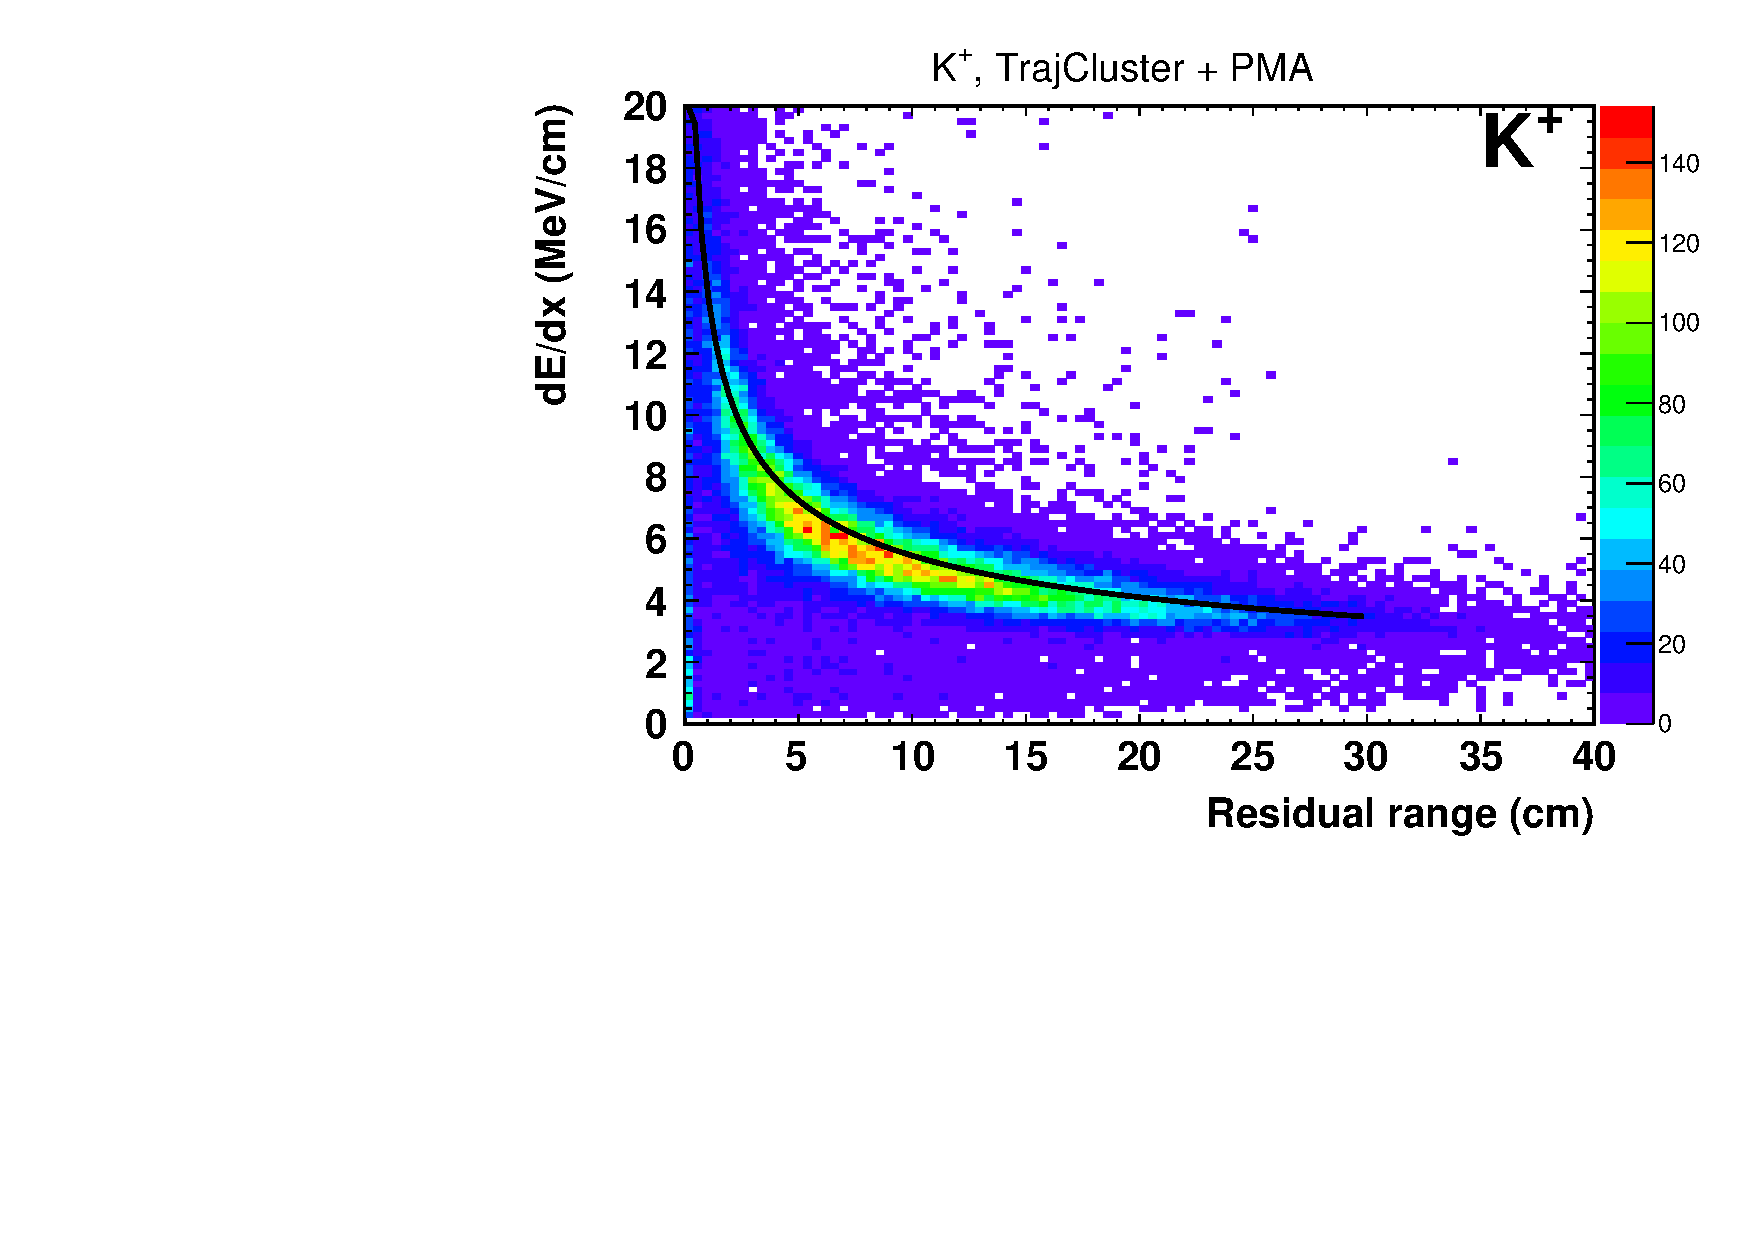
\includegraphics[width=0.5\textwidth]{dedxktc.pdf}}
%\subfloat[$\mu^{+}$]{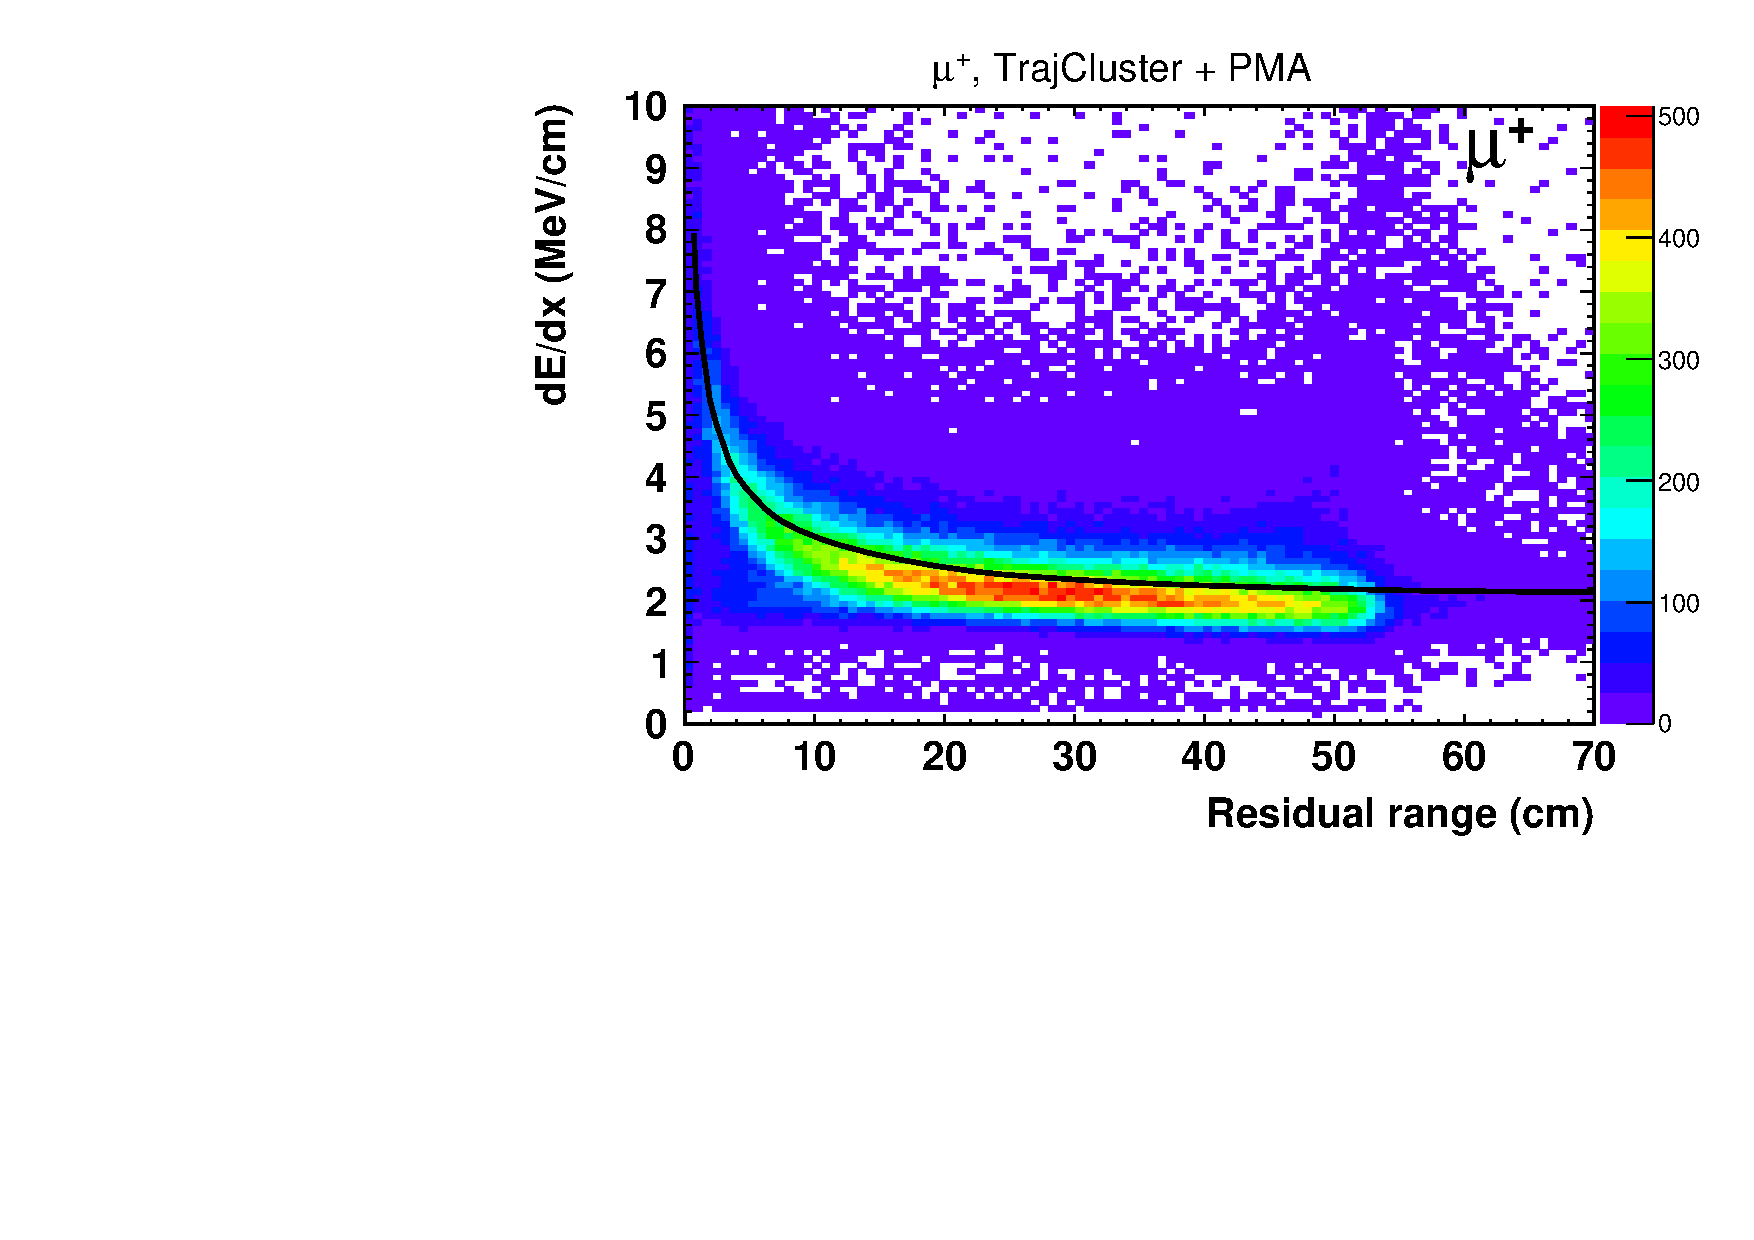
\includegraphics[width=0.5\textwidth]{dedxmutc.pdf}}\\
%\subfloat[$e^{+}$]{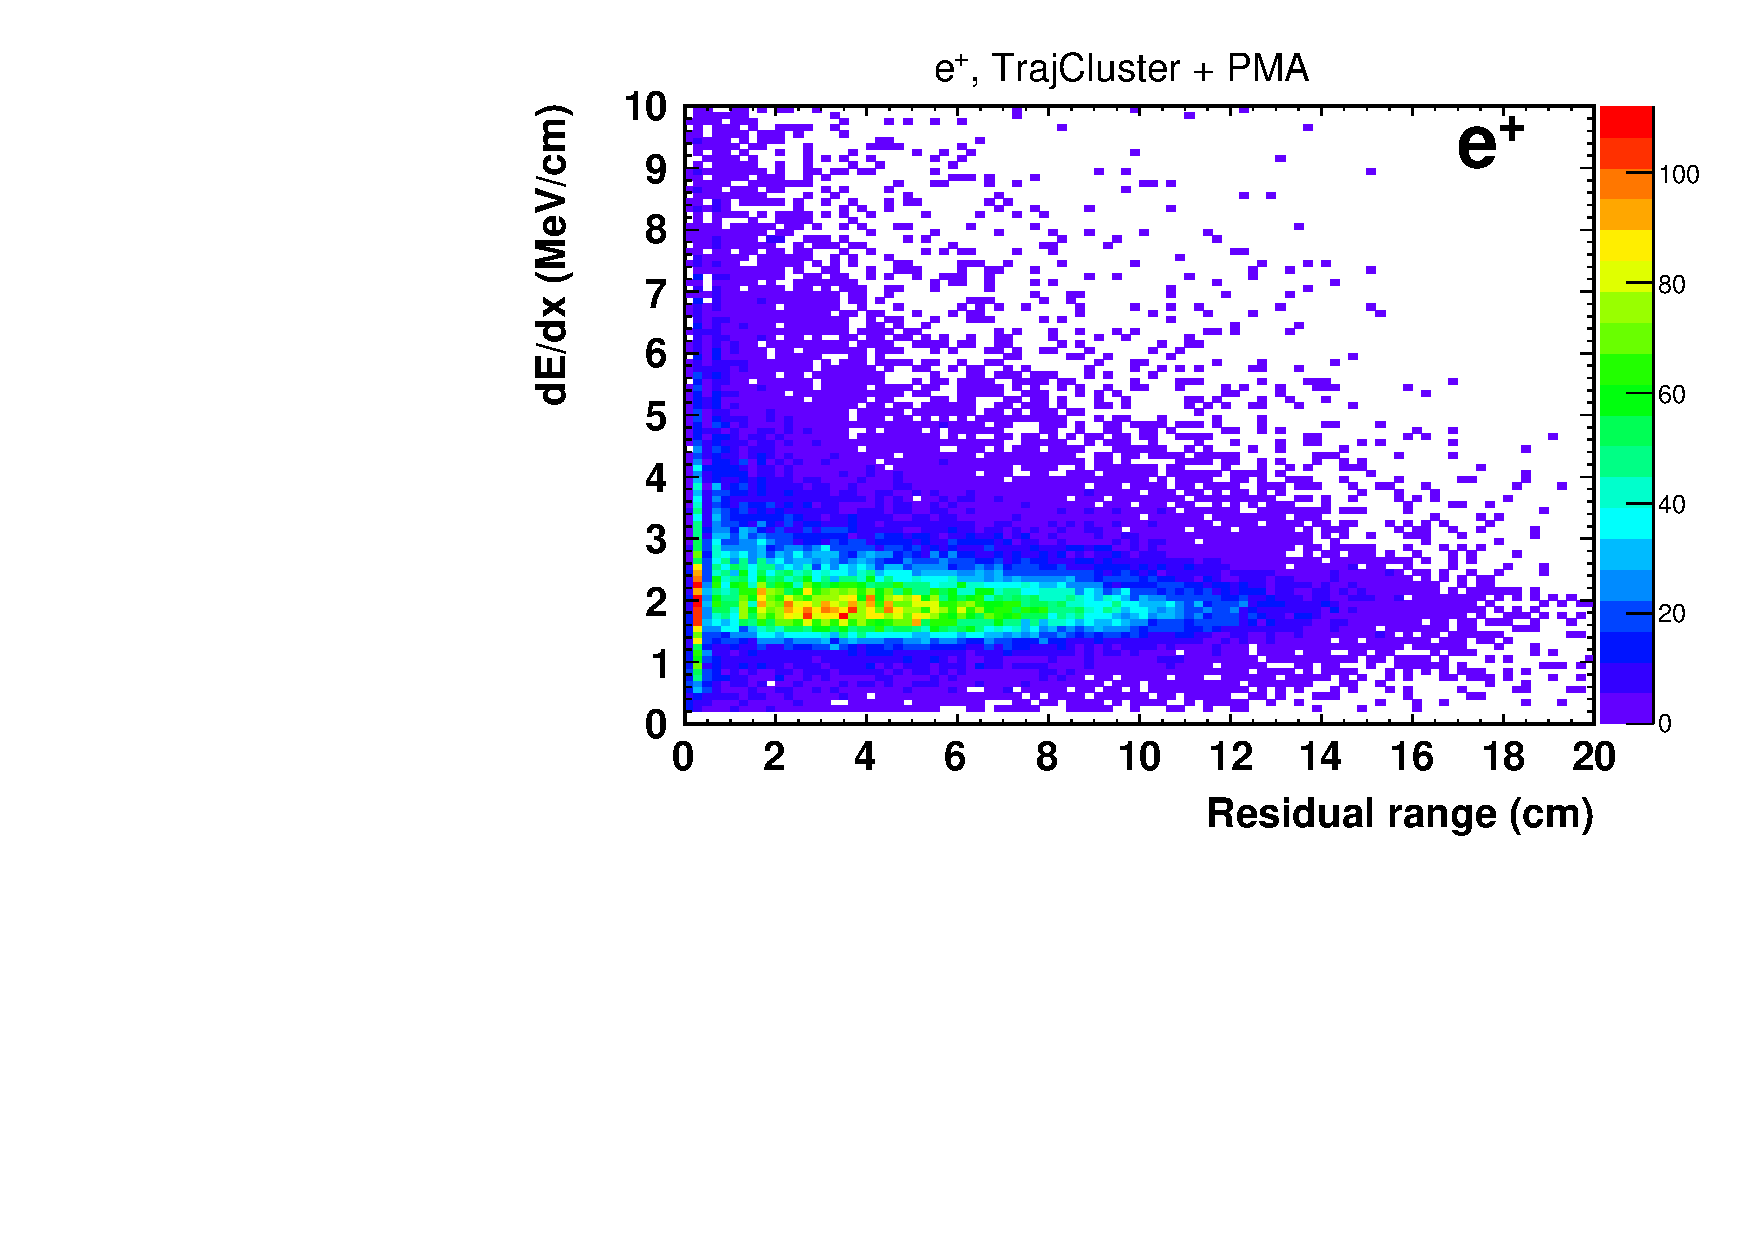
\includegraphics[width=0.5\textwidth]{dedxetc.pdf}}
%\subfloat[$PIDA$]{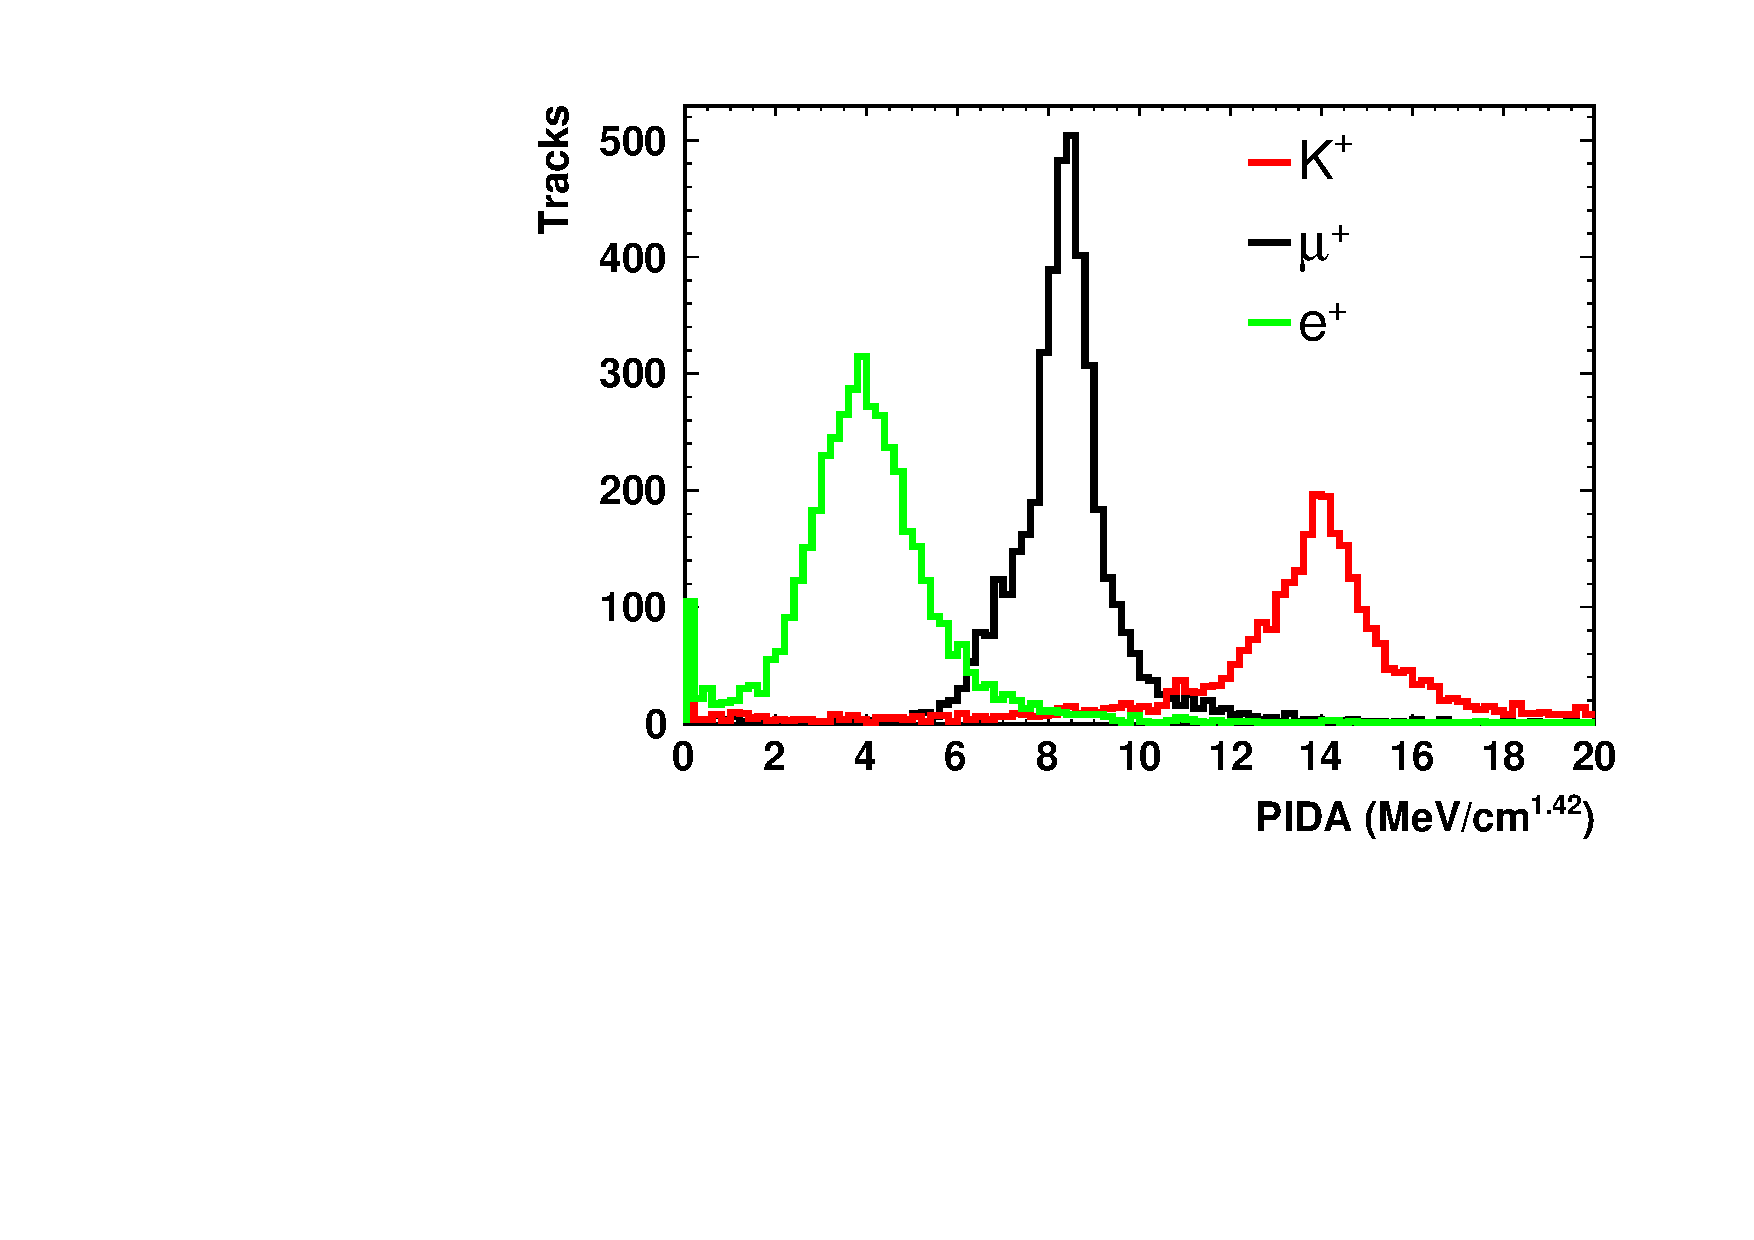
\includegraphics[width=0.5\textwidth]{pidakmue.pdf}}
%\caption{(a)(b)(c): $dE/dx$ as a function of the residual range for reconstructed $K^{+}$, $\mu^{+}$ and $e^{+}$ tracks in proton decay events ($p\rightarrow\bar{\nu}K^{+}$, $K^{+}\rightarrow\mu^{+}\rightarrow e^{+}$). The black curves are theoretical predictions. (d): $PIDA$ distributions of the reconstructed $K^{+}$, $\mu^{+}$ and $e^{+}$ tracks.}
%\label{dedx}
%\end{figure}

\subsection{Wire Cell}

\begin{figure}[!ht]
 \includegraphics[width=0.98\textwidth]{wire-cell-overview.png}
\caption[Overview of \dword{wirecell} reconstruction paradigm]{Overview of\dword{wirecell} reconstruction paradigm, taken from~\cite{ref:wc_talk}. 
See text for more details.}
\label{wire-cell-overview}
\end{figure}


\Dword{wirecell} is a new reconstruction package under development. The current 
status of this reconstruction paradigm is shown in Figure~\ref{wire-cell-overview}. The 
simulation of the induction signal in a LArTPC and the overall signal processing process,
which are general to all reconstruction methods, are described in Sections~\ref{sec:tpc_sim} 
and~\ref{sec:tpc_sp}, respectively. The subsequent reconstruction in \dword{wirecell} adopts 
a different approach from the aforementioned algorithms. Instead of directly performing pattern 
recognition on each of the \twod views (drift time versus wire number), \threed imaging of events 
is obtained with time, geometry, and charge information. This step is independent from 
the event topologies, and the usage of the charge information takes advantage of a unique 
feature of the projection views, as each of the wire plane detects the same 
amount of the ionization electrons under transparency condition. The strong requirement of the time, geometry, and charge 
information provides a natural way to suppress electronic noise
 while combining with successful signal processing maintains high hit efficiency. Details of this step is described in~\cite{Qian:2018qbv}. The subsequent reconstruction involves the object clustering and
TPC and light matching, which has been crucial for selecting neutrino interactions in the 
MicroBooNE experiment~\cite{uboone_wc_note}. The current focus of the \dword{wirecell} algorithm 
development is on the trajectory and $dQ/dx$ fitting, which aims at enabling precision particle
identification in a \lartpc. %Beside these, 
Development of \threed pattern recognition also needs
to be revisited before reaching a complete reconstruction chain. 


\begin{figure}[!ht]
\centering
 \includegraphics[width=0.85\textwidth]{bee_event.png}
\caption{This \threed display shows the full size of the \dword{pdsp} detector (white box) and 
the direction of the particle beam (yellow arrow). Particles from other sources (such as cosmic rays) 
can be seen throughout the white box, while the red box highlights the region of interest: 
in this case, an interaction resulting from the 7 GeV beam particle through the detector. 
The \threed points are obtained using the Space~Point~Solver reconstruction algorithm. This event
can be accessed through interactive web-based event display Bee at \url{https://www.phy.bnl.gov/twister/bee/set/protodune-gallery/event/0/}.}
\label{wire-cell-bee}
\end{figure}

\dword{wirecell} team also created an advanced web-based \threed event display, ``Bee''~\cite{wire-cell-bee}, to aid the reconstruction development and provide interactive visualizations to end users.  Bee, together with \twod Magnify event 
display tools, have played important roles in 
the development of various reconstruction algorithms, including signal processing, \threed event 
imaging, object clustering, TPC and light matching, and trajectory and $dQ/dx$ fitting. The Bee event display 
was also used during the ProtoDUNE data-taking period to stream real-time reconstructed events to the users.
Figure~\ref{wire-cell-bee} shows an example of a data event from the \dword{pdsp} detector~\cite{ref:wc_bee}. 
The full video of this event can be found in~\cite{ref:bee_video}.

%\fixme{The paragraph below is too much technical detail for a physics TDR.  I propose to comment it out.  -- JU}

%The primary software package hosting various \dword{wirecell} reconstruction algorithm is the 
%\dword{wirecell} toolkit (WCT)~\cite{ref:wire_cell_toolkit}, 
%which provides a consistent, 
%ull-featured configuration system based on the Jsonnet \cite{jsonnet} data templating 
%language and its C++ bindings.  Individual component construction and the application of
%configuration data are handled by the toolkit, which allows for dynamic
%construction patterns.  WCT supports a number of component execution models and in particular
%provides one powerful built-in  model that follows the data flow
%programming paradigm.  It connects toolkit components as nodes in a
%directed graph that exchange data along the graph edges.  A flow graph
%may be constructed in C++ or more simply via user configuration. The execution of a WCT 
%flow graph is itself an abstracted component.  Two implementations currently exist.
%One is single-threaded and minimizes memory usage.  The
%second, based on Intel TBB~\cite{tbb} allows for multi-threaded
%concurrent execution of components and exchanges data across graph edges
%%which are 
%implemented as thread-safe queues. The development of WCT follows a toolkit approach
%and is designed to be easily integrated into larger applications. The toolkit makes strong use of 
%abstractions for all public data objects and code units. With a shared library 
%plugin system, the abstract interface implementation is made available to the application
%using the toolkit. Currently, WCT has been integrated into the \dword{art} framework via a
%package in the \dword{larsoft} software suite.  It provides an \dword{art} tool as the primary 
%interface to the WCT as well as a number of WCT components which convert between \dword{larsoft} 
%and WCT data representations. This interface is in regular use to run both MicroBooNE and 
%\dword{pdsp} WCT jobs.



\subsection{Deep Learning}\label{sec:deeplearning}

Deep learning methods are used %There are 
in two main areas of the DUNE event reconstruction. % where . 
Both of these algorithms are based on \dwords{cnn}. 
In recent years \dwords{cnn} have become the method of choice for many image recognition tasks in commerce and industry, and lately have been applied to high energy physics. The \dwords{cnn} contain a series of filters that are applied to the input detector data images in order to extract the features required to classify the images.

\subsubsection{\dword{cnn} for track and shower separation}
The hit-level \dword{cnn} aims to classify each reconstructed hit as either track-like or shower-like by looking at the local region surrounding the hit in (charge, time) coordinates.  The \dword{cnn} is trained using a large number of simulated images with the known true origin of the energy deposits. Once trained, the \dword{cnn} provides the track-like or shower-like classification for each hit object in the event. This algorithm is applied to each readout view in each TPC separately. %The output from the algorithm is shown in Figure \ref{fig:trkshw_CNN_protodune} for a beam interaction in ProtoDUNE-SP. 

\subsubsection{\dword{cnn} for event selection}
The algorithm used for the classification of neutrino interaction types is called the \dword{cvn} and is  based on a \dword{cnn}. The primary goal of the \dword{cvn} is to provide a probability for each neutrino interaction to be \dword{cc}$\,\nu_\mu$, \dword{cc}$\,\nu_e$, \dword{cc}$\,\nu_\tau$ or \dword{nc}. The \dword{cvn} takes three $500\,\times\,500$ pixel images of the neutrino interactions as input, one from each view. The images contain the charge and the peak time of the reconstructed hits and does not use any information beyond the hit reconstruction. The \dword{cvn} is discussed in more detail in the \dword{lbl} chapter of the \dword{tdr} Physics Volume. 

\subsection{Optical Reconstruction}

\subsubsection{Optical Hit Finder}
\label{sec:OpticalHitFinder}
The first step of the DUNE optical reconstruction is reading
individual waveforms from the simulated \dword{pd} electronics
and finding optical hits -- regions of the waveforms containing pulses.
The optical hit contains the optical channel (\dword{sipm}) that the hit
was found on, time corresponding to the hit, its width,
area, amplitude, and number of \phel{}s.


The current DUNE optical-hit-finder algorithm then searches for regions of the waveform
exceeding a certain threshold ($13$ \dword{adc} counts), checking whether that region
is wider than $10$ optical time ticks, and, if it is, calculating the aforementioned
optical-hit parameters for the region (including parts of the waveform around it
that have \dword{adc} values greater than $1$) and recording it as an optical hit.
The number of \phel{}s is calculated by dividing the full area of the hit
by the area of a single-\phel{} pulse.
The pedestal is assumed to be constant and is specified in the hit finder as $1500$ \dword{adc} counts (always correct for the MC).


\subsubsection{Optical Flash Finder}
After optical hits are reconstructed, they are grouped into higher-level objects called optical flashes.
The optical flash contains the time and time width of the flash,
its approximate $y$ and $z$ coordinates (and spatial widths along those axes),
its location and size in the wire planes,
the distribution of \phel{}s across all \dwords{pd},
and the total number of \phel{}s in the flash, among other parameters.

The flash-finding algorithm searches for an increase in \dword{pd} activity
(the number of \phel{}s) in time using information from optical hits
on all photon detectors.
When a collection of hits with the total number of \phel{}s  
greater than or equal to $2$ is found, the algorithm begins creating an optical flash.
It starts with the largest hit and adds hits from the found hit collection 
that lie closer than half the combined widths of the flash under construction
a nd the hit being added to it.
The flash is stored after no more hits can be added to it
and if it has more than two \phel{}s.

The algorithm also estimates spatial parameters of the optical flash
by calculating the number-of-photoelectron-weighted mean and 
root mean square of locations of the optical hits
(defined as centers of \dwords{pd} where those hits were detected)
contained in the flash.

%%%%%%%%%%%%%%%%%%%%%%%%%%%%%%%%%%%%%%%%%%%%%%%%%%%%%%%%%%%%%%%%
\section{Reconstruction Performance}
\label{sec:performance}

An automated reconstruction of the neutrino interaction events in DUNE, often complex topologies with multiple final state particles, is a significant challenge. The currently used chain of \dword{pandora} pattern recognition algorithms %used 
has been tuned for neutrino interactions from the \fnal Booster Neutrino Beam, and it is in the process of being adapted for the wide range of energies of the DUNE \dword{fd}. Despite this fact, and thanks to the reusability of \dword{pandora} algorithms for different single phase \lartpc detectors,  good performance is already achieved with this first-pass pattern recognition. Significant improvements are expected  in the upcoming years with a more dedicated tune of the current algorithms, and the development of new ones, as needed. %according to the necessities of DUNE. 

%The following pages show figures assessing the performance of the current reconstruction. They are the result of the full reconstruction chain on the Monte Carlo simulations described in Section~\ref{sec:tools-mc}: i.e., signal processing, hit finder, disambiguation and Pandora pattern recognition. 
The current reconstruction performance, evaluated using metrics introduced in \ref{sec:Pandora:assessment}, is presented for simulated neutrino interactions in a \single \nominalmodsize \dword{fd} module in \ref{sec:Pandora:DUNEFD}, and for simulated and real data test beam events in \dword{pdsp} in \ref{sec:Pandora:ProtoDUNE}. These results outline the baseline performance on which improvements will continue to be made in the next years. In addition, current results on high-level reconstruction performance are presented in~\ref{sec:Pandora:High}.

\subsection{Pandora Performance Assessment}
\label{sec:Pandora:assessment}
The performance of the \dword{pandora} pattern recognition is assessed by matching reconstructed PFParticles to the simulated \dword{mc} particles (MCParticles). These matches are used to evaluate the efficiency with which MCParticles are reconstructed as PFParticles, and to calculate the completeness and purity of each reconstructed PFParticle. 

\fixme{mc and pfparticles in gloss?}

The following procedure is used to match reconstructed PFParticles with simulated MCParticles:

\begin{itemize}
\item \textit{Selection of MCParticles:} The full hierarchy of true particles is extracted from the simulated neutrino interaction. A list of ``target'' particles is then compiled by navigating through this hierarchy and selecting the final-state ``visible'' particles producing a minimum number of hits (allowed to be: $e^{\pm}$, $\mu^{\pm}$, $\gamma$, $\pi^{\pm}$, $\kappa^{\pm}$, $p$). Any downstream daughter particles are folded in these target particles.
\item \textit{Matching of reconstructed \twod hits to MCParticles:} Each reconstructed \twod hit is matched to the target MCParticle responsible for depositing the most energy within the region of space covered by the hit. The collection of \twod hits matched to each target MCParticle is known as its ``true hits''.
\item \textit{Matching of MCParticles to reconstructed PFParticles:} The reconstructed PFParticles are matched to target MCParticles by analyzing their shared \twod hits. A PFParticle and MCParticle will be matched if the MCParticle contributes the most hits to the PFParticle, and if the PFParticle contains the the largest collection of hits from the MCParticle. The matching procedure is iterative, such that once each set of matched particles has been identified, these PFParticles and MCParticles are removed from consideration when making the next set of matches. 
\end{itemize}

Using the output of this matching scheme, the following performance metrics can be calculated:

\begin{itemize}
\item \textit{Efficiency:} Fraction of MCParticles with a matched PFParticle,
\item \textit{Completeness:} The fraction of \twod hits in a MCParticle that are shared with its matched reconstructed PFParticle, and 
\item \textit{Purity:} The fraction of \twod hits in a PFParticle that are shared with its matched MCParticle.
\end{itemize}

\subsection{Reconstruction Performance in the DUNE \dword{fd}}
\label{sec:Pandora:DUNEFD}

The performance of the \dword{pandora} pattern recognition has been evaluated using a sample of accelerator neutrino interactions simulated using the reference DUNE neutrino energy spectrum and the \nominalmodsize \dword{detmodule} geometry. The following plots show that a good efficiency has already been achieved, and indicate particular regions and channels in which improvements can be made. 

\begin{figure}[!ht]
\centering
\includegraphics[width=0.5\textwidth]{Pandora-ALL_BUT_DIS_HitsEff_Tracks.png}\includegraphics[width=0.5\textwidth]{Pandora-ALL_BUT_DIS_HitsEff_Showers.png}
\includegraphics[width=0.5\textwidth]{Pandora-ALL_BUT_DIS_MomentumEff_Tracks.png}\includegraphics[width=0.5\textwidth]{Pandora-ALL_BUT_DIS_MomentumEff_Showers.png}

\caption[Reconstruction efficiency of \dword{pandora} pattern recognition for a range of final-state particles at the \dword{fd}]{The reconstruction efficiency of the \dword{pandora} pattern recognition obtained for a range of final-state particles produced in all types of accelerator neutrino interactions except deep inelastic ones at DUNE FD. The efficiency is plotted as a function of the total number of \twod hits associated with the final-state MCParticles (summed across all views) on the top row, and as a function of the true momentum of the particle on the bottom row. Plots are shown for track-like particles (left) and shower-like particles (right) of each type leading in the event (in addition to the sub-leading photon $\gamma_2$ added for reference to $\pi^0$ reconstruction).}
\label{pandora_particle_efficiency}
\end{figure}

Figure~\ref{pandora_particle_efficiency} shows the reconstruction efficiency as a function of the number of total true \twod hits and as a function of the true momentum for a range of final-state particles. The typical reconstruction efficiencies obtained for track-like MCParticles ($\mu^{\pm}$, $\pi^{\pm}$, $p$) rise from \SIrange{65}{85}{\%} for simulated particles depositing 100\,hits to \SIrange{85}{100}{\%} for particles with 1000\,hits. It should be emphasized that inefficiencies almost always result from accidental merging of multiple nearby true particles, rather than an inability to cluster hits from a true particle. The reconstruction efficiency for shower-like MCParticles ($e^{-}$,$\gamma$) is a bit lower than the equivalent for track-like particles at lower number of hits, but comparable with $>$100 hits. The case of the sub-leading photon, $\gamma_2$, is particularly challenging given the correlation with the leading photon, $\gamma_1$, in the $\pi^0$ decays, which may result in accidentally merging both photons; therefore a loss of efficiency is expected for this particular channel, subject to improvements. 

Figure~\ref{pandora_completeness_purity} shows distributions of completenesses and purities for a range of final-state particles. In the case of final-state track-like particles, good completeness and purity are %both 
achieved, indicating that the track-based pattern recognition algorithms currently provide a high-quality reconstruction. It can be seen that final-state shower-like particles are typically reconstructed with high purity, but somewhat lower completeness, indicating that, although the shower reconstruction is fairly good already, there is room for addition of new algorithms specifically targeting an increase in shower completeness at DUNE.

For deep inelastic interactions, in which tens of final-state particles are produced, a breakdown such as in Figures~\ref{pandora_particle_efficiency} and~\ref{pandora_completeness_purity} is less representative and informative. Instead, Figure~\ref{pandora_dis} presents an assessment of the reconstruction of such events %is presented 
by comparing the number of reconstructed particles as a function of the number of true final-state particles in the event for \dword{nc} (left) and \dword{cc} (middle) deep inelastic interactions. These distributions are more populated in the diagonal, as they should be for perfect 1:1 reconstruction, indicating a good level of reconstruction of such events up to >5 final-state particles. In addition, the number of reconstructed particles matching the leading lepton in \dword{cc} deep inelastic interactions is also presented (right), which shows a consistently predominant single match for the leading lepton. 

Figure~\ref{pandora_vertex_resolution} shows distributions of the displacements $\Delta x$, $\Delta y$ and $\Delta z$ between the reconstructed and simulated neutrino interaction positions for all types of accelerator neutrino events. It can be seen that, for the vast majority of events, the reconstructed neutrino  interaction vertex lies within $2$\,cm of the \dword{mc} truth in $x$, $y$ and $z$. While the $\Delta x$ and $\Delta y$ distributions are both symmetrical and sharply peaked around the origin, a small forward bias can be seen in the $\Delta z$ distribution. The reason for this bias comes from the fact that the neutrino interaction will be boosted in the forward $z$ direction, so vertex candidates are more likely created at $\Delta z>0$ than $\Delta z\,<\,0$.  

\begin{figure}[!ht]
\centering
\includegraphics[width=0.5\textwidth]{Pandora-ALL_BUT_DIS_Completeness_Tracks_Log.png}\includegraphics[width=0.5\textwidth]{Pandora-ALL_BUT_DIS_Completeness_Showers_Log.png}
\includegraphics[width=0.5\textwidth]{Pandora-ALL_BUT_DIS_Purity_Tracks_Log.png}\includegraphics[width=0.5\textwidth]{Pandora-ALL_BUT_DIS_Purity_Showers_Log.png}
\caption[Completeness (top) and purities (bottom) for a range of final-state track-like  and shower-like particles]{Distributions of completenesses (top) and purities (bottom) for a range of final-state particles divided into track-like (left) and shower-like (right), produced in all types of accelerator neutrino interactions except deep inelastic ones at DUNE FD. }
\label{pandora_completeness_purity}
\end{figure}

\begin{figure}[!ht]
\centering
\includegraphics[width=0.315\textwidth]{Pandora-NCDIS.png}
\includegraphics[width=0.315\textwidth]{Pandora-CCDIS.png}
\includegraphics[width=0.315\textwidth]{Pandora-CCDISLeptonMatches.png}
\caption[Number of reconstructed particles per number of true final-state particles, \dword{cc} and \dword{nc}]{Distributions of number of reconstructed particles as a function of number of true final-state particles in deep inelastic events for neutral-current (left) and charged-current (middle) interactions. In addition, the number of reconstructed particles matching the leading lepton in charged-current deep inelastic interactions is also presented (right).}
\label{pandora_dis}
\end{figure}


\begin{figure}[!ht]
\centering
\includegraphics[width=0.35\textwidth]{Pandora-ALL_INTERACTIONS_VtxDeltaX.png}\includegraphics[width=0.35\textwidth]{Pandora-ALL_INTERACTIONS_VtxDeltaY.png}\includegraphics[width=0.35\textwidth]{Pandora-ALL_INTERACTIONS_VtxDeltaZ.png}
\caption[Displacements between reconstructed and simulated $\nu$ interaction vertices]{The displacements between the reconstructed and simulated neutrino interaction vertices. The distributions are plotted for $x$ (left), $y$ (center) and $z$ (right) and include all types of accelerator neutrino interaction (also deep inelastic events).}
\label{pandora_vertex_resolution}
\end{figure}

\subsection{Reconstruction Performance in \dword{pdsp}}
\label{sec:Pandora:ProtoDUNE}

Further examination of the performance of the \dword{pandora} pattern recognition is provided through studies of the test beam data taken by \dword{pdsp}.  Figure \ref{pandora_protodune_tbrecoeff} shows the reconstruction efficiency for triggered test beam particles as a function of the momentum recorded by the trigger.  The reconstruction efficiency metric folds in many effects, including reconstruction, removal of cosmic ray background and identification of the reconstructed particle as originating from the test beam.  An example of the \dword{pandora} reconstruction output for ProtoDUNE \dword{mc} simulations is shown in Figure~\ref{pandora_protodune_reco}.  A broad agreement between the \dword{mc} simulations and the data can be observed in Figure~\ref{pandora_protodune_tbrecoeff} across the range of momenta considered.  The exceptions to this are: (1) low-momentum events, where the low efficiency for data is due to particles interacting between the trigger and the LArTPC before reaching its active volume, an effect that is not simulated in \dword{mc}, and (2) high-momentum events, where the effect of test beam halo particles appears to be overestimated in the simulation.

\begin{figure}[!ht]
\centering
\includegraphics[width=0.75\textwidth]{./Pandora/ProtoDUNE/BeamParticleEfficiencyVsMomentum.pdf}
\caption[Reconstruction efficiency for triggered test beam particle per particle momentum  and \dword{mc}.]{The efficiency of reconstruction for the triggered test beam particle as a function of the momentum of the test beam particle in (black) data and (red) Monte-Carlo.}
\label{pandora_protodune_tbrecoeff}
\end{figure}

\begin{figure}[!ht]
\centering
\subfloat[]{\label{fig:reco3d}\includegraphics[width=0.75\textwidth]{./Pandora/ProtoDUNE/Reconstruction.pdf}} \\ 
\subfloat[]{\label{fig:recou}\includegraphics[width=0.33\textwidth]{./Pandora/ProtoDUNE/ReconstructionU.pdf}}
\subfloat[]{\label{fig:recov}\includegraphics[width=0.33\textwidth]{./Pandora/ProtoDUNE/ReconstructionV.pdf}}
\subfloat[]{\label{fig:recow}\includegraphics[width=0.33\textwidth]{./Pandora/ProtoDUNE/ReconstructionW.pdf}}
\caption[Pandora reconstruction output for \SI{7}{GeV} \dword{mc} test beam event]{An example of the \dword{pandora} reconstruction output for a 7 GeV Monte Carlo test beam event.  Figure \protect\subref{fig:reco3d} shows the \threed reconstruction output for this event where the correctly reconstructed and tagged triggered test beam particle has been highlighted.  Figures \protect\subref{fig:recou}, \protect\subref{fig:recov} and \protect\subref{fig:recow} show the \twod hits for the reconstructed test beam particle where each coloured cluster of hits represents a different particle in the reconstructed particle hierarchy.}
\label{pandora_protodune_reco}
\end{figure}

The effect of cosmic ray backgrounds and the test beam particle halo on the reconstructed test beam particle efficiency is illustrated in Figure~\ref{fig:pandora_protodune_tbrecoeffbrkdwn}, where the efficiency is shown as a function of the momentum of the triggered particle (\ref{fig:pandora_protodune_tbrecoeffbrkdwn_p}) and the number of hits produced by the triggered particle (\ref{fig:pandora_protodune_tbrecoeffbrkdwn_nhits}).  These figures indicate that the primary loss mechanisms in the test beam particle reconstruction, accounting for $\approx 70\%$ of all inefficiencies, are due to irreducible cosmic ray and test beam halo backgrounds.

\begin{figure}[!ht]
\centering
\subfloat[]{\label{fig:pandora_protodune_tbrecoeffbrkdwn_p}\includegraphics[width=0.5\textwidth]{./Pandora/ProtoDUNE/BeamParticleEfficiencyBreakdownVsMomentum.pdf}}
\subfloat[]{\label{fig:pandora_protodune_tbrecoeffbrkdwn_nhits}\includegraphics[width=0.5\textwidth]{./Pandora/ProtoDUNE/BeamParticleEfficiencyBreakdownVsNHits.pdf}} \\
\subfloat[]{\label{fig:pandora_protodune_tbrecoeffbrkdwn_evt}\includegraphics[width=0.6\textwidth]{./Pandora/ProtoDUNE/EventComposition.pdf}}
\caption[Reconstruction efficiency for test beam particle in \dword{mc} per momentum and hits]{The efficiency of reconstruction for the triggered test beam particle in Monte-Carlo as a function of \protect\subref{fig:pandora_protodune_tbrecoeffbrkdwn_p} the triggered beam momenta and \protect\subref{fig:pandora_protodune_tbrecoeffbrkdwn_nhits} the number of hits made by the triggered particle.  The three curves show the reconstruction efficiency of the triggered test beam particle in isolation (blue), with beam particle halo overlaid (red) and with both beam particle halo and cosmic ray backgrounds overlaid (black).  Figure \protect\subref{fig:pandora_protodune_tbrecoeffbrkdwn_evt} shows the W plane view for a Monte-Carlo event where the triggered beam particle is shown in blue, the beam halo in red and the cosmic ray backgrounds in black.}
\label{fig:pandora_protodune_tbrecoeffbrkdwn}
\end{figure}

Alongside the test beam particle reconstruction metrics, the \dword{pandora} cosmic ray reconstruction has been studied using \dword{pdsp} data. 

Figure \ref{fig:pandora_protodune_cr_n} shows the number of reconstructed cosmic rays per event.  Both data and \dword{mc} have a consistent average number of cosmic rays per event ($\approx\,110$), however the \dword{mc} distribution seems to have a larger tail, which might be due to differences in the cosmic ray profile in the simulation with respect to the data. Figure~\ref{fig:pandora_protodune_cr_recovsmc} shows the number of reconstructed cosmic rays per event as a function of the number of ``target'' reconstructable (as explained in Section~\ref{sec:Pandora:assessment}) cosmic rays per event for \dword{mc} simulation, illustrating that the \dword{pandora} cosmic ray reconstruction is highly efficient.  The \dword{pandora} reconstruction is also able to tag the true time that a cosmic ray passes through the detector, $t_{0}$, should it cross a drift volume boundary, either \dword{cpa} or \dword{apa}.  This allows us to compare the $t_{0}$ distribution for tagged cosmic rays in data and \dword{mc}, shown in Figure \ref{fig:pandora_protodune_cr_t}.  There is excellent agreement between data and \dword{mc} in this instance.  For cosmic ray particles with a $t_{0} \approx 0$, the hits on either side of the \dword{cpa} or \dword{apa} boundary do not require shifting and therefore the algorithm tagging the $t_{0}$ is not activated; this explains the decrease in event fraction for the $t_{0} \approx 0$ bin.  Figure~\ref{fig:pandora_protodune_cr_tres} shows the resolution on the reconstructed $t_{0}$ for \dword{mc}, which indicates that the \dword{pandora} $t_{0}$ tagging is precise to the order of microseconds.  

\begin{figure}[!ht]
\centering
\subfloat[]{\label{fig:pandora_protodune_cr_n}\includegraphics[width=0.5\textwidth]{./Pandora/ProtoDUNE/NumberofReconstructedCosmicRays.pdf}}
\subfloat[]{\label{fig:pandora_protodune_cr_recovsmc}\includegraphics[width=0.357\textwidth]{./Pandora/ProtoDUNE/CRMatchesCosmicRayEvent.pdf}} \\
\caption[Reconstructed cosmic rays per event for data and \dword{mc}]{The number of reconstructed cosmic rays per event is shown in figure \protect\subref{fig:pandora_protodune_cr_n} for data and \dword{mc}.  Figure \protect\subref{fig:pandora_protodune_cr_recovsmc} shows the true number of reconstructable cosmic rays passing through the detector per event plotted against the number of reconstructed cosmic rays for \dword{mc}.}
\label{fig:pandora_protodune_cr_number}
\end{figure}

\begin{figure}[!ht]
\centering
\subfloat[]{\label{fig:pandora_protodune_cr_t}\includegraphics[width=0.5\textwidth]{./Pandora/ProtoDUNE/StitchedT0.pdf}}
\subfloat[]{\label{fig:pandora_protodune_cr_tres}\includegraphics[width=0.5\textwidth]{./Pandora/ProtoDUNE/Pandora_Resolution_T0_5GeV_Beam_Cosmic_SpaceChargeEffectOn.png}}
\caption[Distribution of reconstructed $t_{0}$ for cosmic rays]{Figure \protect\subref{fig:pandora_protodune_cr_t} shows the distribution of the reconstructed $t_{0}$ for cosmic rays crossing the \dword{cpa} in both data and \dword{mc}, while Figure \protect\subref{fig:pandora_protodune_cr_tres} shows the resolution on the reconstructed $t_{0}$ in \dword{mc}.}
\label{fig:pandora_protodune_cr_t0}
\end{figure}
%\subsection{Calorimetry Reconstruction in Single-Phase ProtoDUNE}
%\label{sec:caloprotodune}


\subsection{High-Level Reconstruction}
\label{sec:Pandora:High}

This section presents a series of studies to illustrate the results of current efforts on high-level reconstruction, analyzing different reconstructed quantities and calorimetric variables for tracks and showers. After the pattern recognition stage provided by \dword{pandora}, further fits to the reconstructed \threed particles can be made in order to characterize their properties. For the moment, the results presented here use only the output provided by \dword{pandora}, which includes a first pass of high-level reconstruction to build these objects. For tracks, \dword{pandora} sliding linear fits are used to calculate the trajectory of the particle, and for showers, a principal component analysis (PCA)\fixme{gloss?} is used to estimate directions and opening angles. 

\subsubsection{Tracks}
\label{sec:Pandora:High:Tracks}

Basic quantities that can be explored in the high-level reconstruction of track-like objects are length and direction (Figure~\ref{fig:pandora_dunefd_highlevel_reco}). Figure~\ref{fig:pandora_dunefd_highlevel_reco_length} shows the difference between reconstructed and true particle length (\threed distance between start and end positions) in simulated track-like particles of various types in the \dword{fd}. The same \dword{fd} simulated events are interrogated to produce Figure~\ref{fig:pandora_dunefd_highlevel_reco_angle}, which shows the angle between the reconstructed and the true \threed direction of the track.   

\begin{figure}[!ht]
\centering
\subfloat[]{\label{fig:pandora_dunefd_highlevel_reco_length}
%\includegraphics[width=0.25\textwidth]{./placeholder.png}
}
\subfloat[]{\label{fig:pandora_dunefd_highlevel_reco_angle}
%\includegraphics[width=0.25\textwidth]{./placeholder.png}
}
\caption[Distribution of reconstructed-true length for different track-like particles]{Distribution of reconstructed - true length (\threed distance between start and end positions) for different track-like particles \protect\subref{fig:pandora_dunefd_highlevel_reco_length}, and angle between the reconstructed and the true \threed direction of the tracks \protect\subref{fig:pandora_dunefd_highlevel_reco_angle} in simulated \dword{fd} events.}
\label{fig:pandora_dunefd_highlevel_reco}
\end{figure}

A number of these variables can be also explored in real data taken by the \dword{pdsp} detector. In the case of the direction, the distribution of the opening angle between the expected direction and a fit to the start of the reconstructed test beam particle in \dword{pdsp} is shown for both data and \dword{mc} in Figure~\ref{fig:pandora_protodune_openingangle}.    Figure~\ref{fig:pandora_protodune_vertex} presents a measurement of the test beam particle interaction vertex by comparing the end point of the primary test beam particle track and the interaction vertex, obtained using the start point of the reconstructed daughter particles emerging from the interaction point, for \dword{pdsp} data and \dword{mc} events. 

\begin{figure}[!ht]
\centering
\includegraphics[width=0.75\textwidth]{./Pandora/ProtoDUNE/BeamParticleOpeningAngle.pdf}
\caption[distribution of opening angle between expected direction and fit to reconstructed test beam particle, data and \dword{mc}]{The distribution of the opening angle between the expected direction and a fit to the start of the reconstructed test beam particle for both data and \dword{mc}.  For data, the expected direction is given by the trigger, while for the \dword{mc} the truth information is used.  The discrepancy between the opening angles for data and \dword{mc}, particularly for low angles, is likely to be due to deviations in the expected direction for data as the particle travels from the trigger to the TPC active volume.}
\label{fig:pandora_protodune_openingangle}
\end{figure}



\begin{figure}[!ht]
\centering
%\includegraphics[width=0.25\textwidth]{./placeholder.png}
\caption{Resolution on the test beam particle interaction vertex on \dword{protodune} data and \dword{mc} events, calculated comparing the end point of the primary test beam particle track and the interaction vertex, obtained using the start point of the reconstructed daughter particles emerging from the interaction point.}
\label{fig:pandora_protodune_vertex}
\end{figure}

 A data-driven measurement of the resolution of the reconstruction of track-like particles can be done by splitting the track in two parts, fitting both independently and comparing the results of both fits. This is presented in Figure~\ref{fig:pandora_protodune_trackres} for \dword{pdsp} cosmic tracks.
 
\begin{figure}[!ht]
\centering
%\includegraphics[width=0.25\textwidth]{./placeholder.png}
\caption[Data-driven resolution measurement of the track reconstruction for \dword{pdsp} cosmic ray data]{Data-driven measurement of the resolution of the track reconstruction for \dword{pdsp} cosmic ray data, done by splitting the cosmic ray muon track in two parts, fitting both independently and comparing the results of both fits.}
\label{fig:pandora_protodune_trackres}
\end{figure}

%Distributions of dEdx for stopping muons and protons are shown in Figures\ref{fig:pandora_protodune_mu} and \ref{fig:pandora_protodune_proton} respectively... 
Cosmic ray muons in the \dword{pdsp} detector are also used to calibrate the detector nonuniformity and determine the absolute energy scale. Cathode crossing cosmic-ray muons with $t_{0}$ information are used to correct for the attenuation effect caused by impurities in the \lar. Stopping cosmic ray muons are used to determine the calorimetry constants that convert the calibrated \dword{adc} counts to the number of electrons so that the $dE/dx$ versus residual distributions match the expectation, as shown in Figures~\ref{fig:muon_dedx_resrange_run5387} and~\ref{fig:muon_dedx_resrange_sce} for \dword{pdsp} data and \dword{mc} simulation with space charge effects after calibration. The data $dE/dx$ distribution has better resolution because the purity in data is better than in the simulation. 

\begin{figure}[!ht]
\centering
\subfloat[]{\label{fig:muon_dedx_resrange_run5387}\includegraphics[width=0.33\textwidth]{muon_run5387_dedx.pdf}}
\subfloat[]{\label{fig:muon_dedx_resrange_sce}\includegraphics[width=0.33\textwidth]{muon_sce_mc.pdf}}
\subfloat[]{\label{fig:muon_comparison_dedx_sce_data}\includegraphics[width=0.33\textwidth]{muon_dEdx.pdf}}
\caption[Stopping muon $dE/dx$ distributions for the \dword{pdsp} cosmic data and \dword{mc}]{Stopping muon $dE/dx$ distributions for the \dword{pdsp} cosmic data and \dword{mc}. The red curves in \protect\subref{fig:muon_dedx_resrange_run5387} and \protect\subref{fig:muon_dedx_resrange_sce} are the expected most probable value of $dE/dx$ versus residual range.}
\label{fig:pandora_protodune_mu}
\end{figure}

The same attenuation correction and calorimetry constants are applied to the beam proton data and \dword{mc} and the resulting $dE/dx$ distributions are shown in Figure~\ref{fig:pandora_protodune_proton}. The data and \dword{mc} $dE/dx$ distributions agree well. Discrepancy with expectation is observed in the large residual range region, which corresponds to the beam entering point on the TPC front face where space charge effects are large. Good progress is being made on the space charge effects calibration, which will lead to more accurate $dE/dx$ measurements.
\begin{figure}[!ht]
\centering
\subfloat[]{\label{fig:proton_dedx_resrange_run5387}\includegraphics[width=0.33\textwidth]{proton_dedx_resrange_run5387.pdf}}
\subfloat[]{\label{fig:proton_dedx_resrange_sce}\includegraphics[width=0.33\textwidth]{proton_dedx_resrange_sce.pdf}}
\subfloat[]{\label{fig:proton_comparison_dedx_sce_data}\includegraphics[width=0.33\textwidth]{proton_comparison_dedx_sce_data.pdf}}
\caption[Proton $dE/dx$ distributions for the \dword{pdsp} 1 GeV beam data and \dword{mc}]{Proton $dE/dx$ distributions for the \dword{pdsp} 1 GeV beam data and \dword{mc}. The red curves in \protect\subref{fig:proton_dedx_resrange_run5387} and \protect\subref{fig:proton_dedx_resrange_sce} are the expected most probable value of $dE/dx$ vs residual range.}
\label{fig:pandora_protodune_proton}
\end{figure}


\subsubsection{Showers}
\label{sec:Pandora:High:Showers}

For shower-like particles, different quantities are presented for DUNE \dword{fd} simulated events in Figure~\ref{fig:pandora_dunefd_showers}. The first row of plots shows $dE/dx$ calculated at the start of the shower (within the first \SI{2}{cm} from its start point) for electrons (Figure~\ref{fig:pandora_dunefd_showers_dEdx_e}) and photons (Figure~\ref{fig:pandora_dunefd_showers_dEdx_ph}) %This will need further explanation of features observed for sure - to do when I have the final plot (i.e. might be only non DIS events, collection plane, etc.  
The difference between the true and reconstructed energy is presented in Figure~\ref{fig:pandora_dunefd_showers_E_e} for electrons and in Figure~\ref{fig:pandora_dunefd_showers_E_ph} for photons. Finally the opening angle between the true and reconstructed direction of the shower is shown in Figure~\ref{fig:pandora_dunefd_showers_angle_e} for electrons and Figure~\ref{fig:pandora_dunefd_showers_angle_ph}  for photons. 

\begin{figure}[!ht]
\centering
\subfloat[]{\label{fig:pandora_dunefd_showers_dEdx_e}
%\includegraphics[width=0.25\textwidth]{./placeholder.png}
}
\subfloat[]{\label{fig:pandora_dunefd_showers_dEdx_ph}
%\includegraphics[width=0.25\textwidth]{./placeholder.png}
}

\subfloat[]{\label{fig:pandora_dunefd_showers_E_e}
%\includegraphics[width=0.25\textwidth]{./placeholder.png}
}
\subfloat[]{\label{fig:pandora_dunefd_showers_E_ph}
%\includegraphics[width=0.25\textwidth]{./placeholder.png}
}

\subfloat[]{\label{fig:pandora_dunefd_showers_angle_e}
%\includegraphics[width=0.25\textwidth]{./placeholder.png}
}
\subfloat[]{\label{fig:pandora_dunefd_showers_angle_ph}
%\includegraphics[width=0.25\textwidth]{./placeholder.png}
}
\caption[Distributions of $dE/dx$, energy and angle between true and reconstructed directions for $e^-$s and $\gamma$s]{Distributions of $dE/dx$ (top), energy (middle) and angle (bottom) between true and reconstructed directions for electrons (left) and photons (right).}
\label{fig:pandora_dunefd_showers}
\end{figure}


Using \dword{pdsp} electron test beam data, some of the previous quantities can be computed for real data as well. This is shown in Figure~\ref{fig:pandora_protodune_showers_dEdx_e} for $dE/dx$, and in Figure~\ref{fig:pandora_protodune_showers_dEdx_e} for energy in each of the different momentum ranges.   

\begin{figure}[!ht]
\centering
\subfloat[]{\label{fig:pandora_protodune_showers_dEdx_e}
%\includegraphics[width=0.25\textwidth]{./placeholder.png}
}
\subfloat[]{\label{fig:pandora_protodune_showers_E_e}
%\includegraphics[width=0.25\textwidth]{./placeholder.png}
}
\caption[Distributions of $dE/dx$, energy and angle between true and reconstructed directions for $e^-$s and $\gamma$s????]{
Distributions of $dE/dx$ (left) and energy (right) of showers for electron test beam data at ProtoDUNE single phase detector. }
\label{fig:pandora_protodune_showers}
\end{figure}

\clearpage
%%%%%%%%%%%%%%%%%%%%%%%%%%%%%%%%%%%%%%%%%%%%%%%%%%%%%%%%%%%
%%%%%%%%%%%%%%%%%%%%%%%%%%%%%%%%%%%%%%%%%%%%%%%%%%%%%%%%%%%
%placeholder
\section{DUNE Calibration Strategy}
\label{sec:phys-calib-strat}


The DUNE \dword{fd} presents a unique challenge for calibration in many ways. It differs from existing \dword{lbl} neutrino detectors and existing \dwords{lartpc} because of its size -- the largest \dword{lartpc} ever constructed -- but also because of its deep underground location. 
The DUNE \dword{nd}, which we expect to include a \dword{lartpc}, will also differ from previous experiments (e.g., MINOS and \nova). In particular, while the ND will be highly capable, pile-up and readout will be different, and this may complicate extrapolation of all relevant detector characteristics.

As for any \lartpc, full exploitation of DUNE's capability for precision tracking and calorimetry requires a detailed understanding of the detector response. The inherently highly convolved detector response model and the strong correlations that exist between various calibration quantities make this challenging. 
For example, the determination of energy associated with an event of interest will depend on the simulation model, associated calibration parameters, non-trivial correlations between the parameters, and spatial and temporal dependence of those parameters caused by the non-static nature of the \dword{fd}. 
Changes can be abrupt (e.g., noise, a broken resistor in the \dword{fc}), or ongoing (e.g., exchange of fluid through volume, ion accumulation).

Convincing physics measurements will require a demonstration that the overall detector response is well understood. The systematic uncertainties for the \dword{lbl} and low-energy (\dword{snb}) program will determine the required precision on dedicated calibration systems.
The calibration program must provide measurements at the few-percent-or-better level stably across an enormous volume and over a long period of time, and provide sufficient redundancy.

This section describes the current calibration strategy for DUNE that uses existing sources of particles, external measurements, and dedicated external calibration hardware systems. Existing calibration sources for DUNE include beam or atmospheric neutrino-induced samples, cosmic rays, argon isotopes, and instrumentation devices such as \lar purity and temperature monitors. Dedicated calibration hardware systems currently include laser and pulsed neutron system (PNS).
%and radioactive source deployment systems. %%KM removed
The responsibility of these hardware systems and assessment of alternative calibration system designs fall under the joint \dword{sp} and \dword{dp} calibration consortium. External measurements by \dword{protodune} and SBN will validate techniques, tools and the design of systems applicable to the DUNE calibration program;  \dword{protodune} will also perform essential measurements of charged particle interactions in \dword{lar}.
%and are essential to the success of the overall calibration program.  %%KM I removed essential SBN 

Under current assumptions, the calibration strategy described in this document is applicable to both \dwords{spmod} and \dwords{dpmod}. %Sections~\ref{sec:phys-calib-req} and \ref{sec:phys-calib-approach} briefly describe the physics-driven calibration requirements, including the calibration sources and the systems required at the different stages of the experiment. 
Section~\ref{sec:phys-calib-req} briefly describes the physics-driven calibration requirements. 
The nominal \dword{dune} \dword{fd} calibration design is described in Section~\ref{sec:phys-calib-sources}. Finally,
%Section~\ref{sec:phys-calib-sum} provides a summary along with future plans for calibration.
Section \ref{sec:phys-calib-approach} describes a staging plan for calibration
%the calibration development plan 
from after the \dword{tdr} through to the operation of the experiment including design validation at \dword{protodune}.
%, to provide context for the systems required at the different stages of the experiment.

%KM: Older text 
\begin{comment}
The DUNE \dword{fd} presents a unique challenge for calibration in many ways. It differs from existing \dword{lbl} neutrino detectors and existing \dwords{lartpc} because of its size -- the largest \dword{lartpc} ever constructed -- but also because of its deep underground location. 
The DUNE \dword{nd}, which we expect to include a \dword{lartpc}, will also differ from previous experiments (e.g., MINOS and \nova). Pile-up and readout issues  may complicate extrapolation of detector characteristics.

As for any \lartpc, full exploitation of DUNE's capability for precision tracking and calorimetry requires a detailed understanding of the detector response. The inherently highly convolved detector response model and the strong correlations that exist between various calibration quantities make this challenging. 
For example, the determination of energy associated with an event of interest will depend on the simulation model, associated calibration parameters, non-trivial correlations between the parameters, and spatial and temporal dependence of those parameters caused by the non-static nature of the \dword{fd}. 
Changes can be abrupt (e.g., noise, a broken resistor in the \dword{fc}), or ongoing (e.g., exchange of fluid through volume, ion accumulation).

Convincing physics measurements will require a demonstration that the overall detector response is well understood. The systematic uncertainties for the \dword{lbl} and low-energy (\dword{snb}) program will determine the required precision on each calibration parameter. 
The calibration program must provide measurements at the few-percent-or-better level stably across an enormous volume and over a long period of time, and provide sufficient redundancy.

This section describes the current calibration strategy for DUNE that uses existing sources of particles, external measurements, and dedicated external calibration hardware systems. Existing calibration sources for DUNE include beam or atmospheric neutrino-induced samples, cosmic rays, argon isotopes, and instrumentation devices such as \lar purity and temperature monitors. Dedicated calibration hardware systems currently include laser, neutron and radioactive source deployment systems. The responsibility of these hardware systems fall under the joint \dword{sp} and \dword{dp} calibration consortium. External measurements by \dword{protodune} and SBND  will validate techniques, tools and the design of systems applicable to the DUNE calibration program and are essential to the success of the overall calibration program. 

Under current assumptions, the calibration strategy described in this document is applicable to both \dwords{spmod} and \dwords{dpmod}. Sections~\ref{sec:phys-calib-req} and \ref{sec:phys-calib-approach} briefly describe the physics-driven calibration requirements, including the calibration sources and the systems required at the different stages of the experiment. The nominal \dword{dune} \dword{fd} calibration design is described in Section~\ref{sec:phys-calib-sources}. Finally, Section~\ref{sec:phys-calib-sum} provides a summary along with future plans for calibration.
\end{comment}

%%%%%%%%%%%%%%%%%%%%%%%%%%%%%%%%%%%%%%%%%%%%%%%%%%%%%%%


\subsection{Physics-driven Calibration Requirements}
\label{sec:phys-calib-req}


To perform adequate calibrations the physics processes that lead to the formation of the signals required for DUNE's broad physics program and detector effects that influence their propagation must be carefully understood, as they ultimately affect the detector's energy response. 
Other categories of effects, such as the neutrino interaction model or reconstruction pathologies, can impact measurements of physical quantities. These other effects are beyond the scope of the \dword{fd} calibration effort and would only lead to a higher overall error budget.

\subsubsection{\dword{lbl} physics}
\label{sec:phys-calib-lbl}
In the physics volume of the DUNE \dword{cdr}~\cite{Acciarri:2015uup}, Figure~3.23 shows that increasing the uncertainties on the \nue event rate from \num{2}\% overall to \num{3}\% results in a \num{50}\% longer run period to achieve a 5$\sigma$ determination of \dword{cpv} for 50\% of its possible values. 
The \dword{cdr} also assumes that the fiducial volume is known to the 1\% level. Thus, calibration information needs to provide an approximately 1-2\% understanding of normalization 
and position resolution within the detector. Later studies~\cite{ebias} expanded the simple treatment of energy  presented above. In particular, \num{1}\% bias on the lepton energy has a significant impact on the sensitivity to \dword{cpv}. 
%
A \num{3}\% bias in the hadronic state (excluding neutrons) is important, as the inelasticity  distribution for neutrinos and antineutrinos is quite different.  Different fractions of their energies go into the hadronic state. Finally, while studies largely consider a single, absolute energy scale, DUNE will need to monitor and correct relative spatial differences across the enormous DUNE \dword{fd} volume; this is also true for time-dependent changes. 

A number of in situ calibration sources will be required to address these broad range of requirements. 
Michel electrons, neutral pions and radioactive sources (both intrinsic and external) are needed for calibrating detector response to electromagnetic activity in the tens-to-hundreds of MeV energy range. Stopping protons and muons from cosmic rays or beam interactions form an important calibration source for calorimetric reconstruction and particle identification. 
\Dword{protodune}, as a dedicated test beam experiment, provides important measurements to characterize and validate particle identification strategies in a \SI{1}{kt}-scale detector and is an essential input to the overall program. Dedicated calibration systems, like lasers, will be useful to provide in situ full-volume measurements of \efield distortions. 
Measuring the strength and uniformity of the \efield is a key aspect of calibration, as  estimates of calorimetric response and \dword{pid} depend on the \efield through recombination. The stringent physics requirements on energy scale and fiducial volume also put similarly stringent requirements on detector physics quantities such as \efield, drift velocity, electron lifetime, and the time dependencies of these quantities; this is discussed in more detail in 
%the calibration chapter of the \dword{sp} volume of the \dword{tdr} \fixme{reference SP TDR; SG: chapters in different volumes cannot be cross linked, so we just need to mention the chapter and the volume of the TDR and that is it. I added this in.} and 
the dedicated laser system discussion under Section~\ref{sec:phys-calib-hardware}.

\subsubsection{\dword{snb} and low-energy neutrino physics}
%The supernova signal will include a electron, photon and neutron (capture) components. 
A combination of 6~MeV (direct neutron capture response), 9~MeV (peak visible $\gamma$-energy of interest to \dword{snb} and $^{8}B$/hep solar neutrinos), 15~MeV (upper visible energy of $^{8}B$/hep solar neutrinos) and $\sim$30~MeV (decay electrons) is needed to map the low energy response. Supernova signal events present specific reconstruction and calibration challenges, and observable energy is shared between different charge clusters and types of energy depositions. In particular, the supernova signal will have a low-energy electron, gamma and neutron capture component, and each needs to be characterized. As discussed further in Section~\ref{ch:snb-lowe}, primary requirements for this physics include 
(1) calibration of absolute energy scale and energy resolution, which is important for resolving spectral features of \dword{snb} events;
(2) calibration of time and light yield response of optical photon detectors;  
(3) absolute timing of events;  
(4) measurement of trigger efficiency at low energies;  and 
(5) understanding of detector response to radiological backgrounds. Further details on the the necessary energy scale, energy resolution and trigger efficiency targets needed can be in Ref\fixme{add citation from Kate S. after her section is done.}.
Potential calibration sources in this energy range include Michel electrons from muon decays (successfully utilized by ICARUS and \dword{microboone}~\cite{Acciarri:2017sjy}), which have a well known spectrum up to $\sim\,$\SI{50}{\MeV}.
Photons from neutral pion decay (from atmospheric and beam induced $\pi^0$) will provide an overall energy scale between \SI{50}{\MeV} and \SI{100}{\MeV}, in addition to cosmic ray muon energy loss. 
However, the limited statistical power of those samples (see Table~\ref{tab:cosmic-ray-calib-rates}) mean that it is not possible for these samples to provide the energy scale or resolution at the spatial and temporal granularity needed.
The pulsed neutron system can provides a source of direct neutron capture across the entire DUNE volume, providing a timing and energy calibration.
%removing the laser part here since not relevant?
%the laser system is timed as well. 
The proposed radioactive source system provides an in situ source of the electrons and de-excitation $\gamma$ rays, which are directly relevant for physics signals from \dword{snb} or $^{8}B$ solar neutrinos. These two systems (discussed in more detail in Section~\ref{sec:phys-calib-hardware}) can provide calibrations of photon, electron, and neutron response for energies below \SI{10}{\MeV}, where photons and electrons may have very different characteristics in \dword{lar}.
%It is more challenging to find ``standard candles'' between \SI{50}{Mev} and \SI{100}{\MeV}, beyond cosmic ray muon energy loss.
%SG removing the below sentence since this is mentioned in at least two other places so no need to mention it here under SNB.
%\Dword{protodune} is a test bed for the planned systems and any additional systems or alternative designs being considered.
%, alternative calibration strategies. 

%One can imagine also ancillary studies of detector response using detectors such as \lariat~\cite{Cavanna:2014iqa}, \dword{microboone}~\cite{Acciarri:2016smi}, and SBND~\cite{Antonello:2015lea}.

\subsubsection{Nucleon decay and other exotic physics}
The calibration needs for nucleon decay and other exotic physics are comparable to those for the \dword{lbl} program, as listed in Section~\ref{sec:phys-calib-lbl}. Signal channels for light \dword{dm} and sterile neutrino searches will be \dword{nc} interactions that are background to the \dword{lbl} physics program. 
Based on the widths of $dE/dx$-based metrics of \dword{pid}, qualitatively, we need to calibrate $dE/dx$ across all drift and track orientations at the few-percent level, similar to the \dword{lbl} effort.


%Older text
\begin{comment}

To perform adequate calibrations the physics processes that lead to the formation of the signals required for DUNE's broad physics program, and the detector effects that influence their propagation, must be carefully understood, as they ultimately affect the detector's energy response. 
Other categories of effects, such as the neutrino interaction model or reconstruction pathologies, can impact measurements of physical quantities. These other effects are beyond the scope of the \dword{fd} calibration effort and would only lead to a higher overall error budget.


\subsubsection{Physics Case Studies}

\paragraph{\dword{lbl} physics}
\label{sec:phys-calib-lbl}
In the physics volume of the DUNE \dword{cdr}~\cite{Acciarri:2015uup}, Figure~3.23 shows that increasing the uncertainties on the \nue event rate from \num{2}\% overall to \num{3}\% results in a \num{50}\% longer run period to achieve a 5$\sigma$ determination of \dword{cpv} for 50\% of its possible values. 
The \dword{cdr} also assumes that the fiducial volume is known to the 1\% level. Thus, calibration information needs to provide an approximately 1-2\% understanding of normalization 
and position resolution within the detector. Later studies~\cite{ebias} expanded the simple treatment of energy  presented above. In particular, \num{1}\% bias on the lepton energy has a significant impact on the sensitivity to \dword{cpv}. 
%
A \num{3}\% bias in the hadronic state (excluding neutrons) is important, as the inelasticity  distribution for neutrinos and antineutrinos is quite different.  Different fractions of their energies go into the hadronic state. Finally, while studies largely consider a single, absolute energy scale, DUNE will need to monitor and correct relative spatial differences across the enormous DUNE \dword{fd} volume; this is also true for time-dependent changes. 

A number of in situ calibration sources will be required to address these broad range of requirements. 
Michel electrons, neutral pions and radioactive sources (both intrinsic and external) are needed for calibrating detector response to electromagnetic activity in the tens-to-hundreds of MeV energy range. Stopping protons and muons from cosmic rays or beam interactions form an important calibration source for calorimetric reconstruction and particle identification. 
\Dword{protodune}, as a dedicated test beam experiment, provides critical measurements to characterize and validate particle identification strategies in a \SI{1}{kt}-scale detector and is an essential input to the overall program. Dedicated calibration systems, like lasers, will be useful to provide in situ full-volume measurements of \efield distortions. 
Measuring the strength and uniformity of the \efield is a key aspect of calibration, as  estimates of calorimetric response and \dword{pid} depend on the \efield through recombination. The stringent physics requirements on energy scale and fiducial volume also put similarly stringent requirements on detector physics quantities such as \efield, drift velocity, electron lifetime, and the time dependencies of these quantities. 

\paragraph{\dword{snb} and low-energy neutrino physics}
These signal events present specific reconstruction and calibration challenges, and observable energy is shared between different charge clusters and types of energy depositions. Primary requirements for this physics include 
(1) calibration of absolute energy scale and an understanding and improvement to the nominal 20\% energy resolution, which is important for resolving spectral features of \dword{snb} events;
(2) calibration of time and light yield response of optical photon detectors;  
(3) absolute timing of events;  
(4) measurement of trigger efficiency at low energies;  and 
(5) understanding of detector response to radiological backgrounds. 
Potential calibration sources in this energy range include Michel electrons from muon decays (successfully utilized by ICARUS and \dword{microboone}~\cite{Acciarri:2017sjy}), which have a well known spectrum up to $\sim\,$\SI{50}{Mev}. Radiological sources provide calibrations of photon, electron, and neutron response for energies below \SI{10}{\MeV}. 
It is more challenging to find ``standard candles'' between \SI{50}{Mev} and \SI{100}{\MeV}, beyond cosmic ray muon energy loss. \Dword{protodune} could potentially be a test bed for various calibration strategies. One can imagine also ancillary studies of detector response using detectors such as \lariat~\cite{Cavanna:2014iqa}, \dword{microboone}~\cite{Acciarri:2016smi}, and SBND~\cite{Antonello:2015lea}.


\paragraph{Nucleon decay and other exotic physics}
The calibration needs for nucleon decay and other exotic physics are comparable to those for the \dword{lbl} program, as listed in Section~\ref{sec:phys-calib-lbl}. Signal channels for light \dword{dm} and sterile neutrino searches will be \dword{nc} interactions that are background to the \dword{lbl} physics program. 
Based on the widths of $dE/dx$-based metrics of \dword{pid}, qualitatively, we need to calibrate $dE/dx$ across all drift and track orientations at the few-percent level or better, similar to the \dword{lbl} effort.
\end{comment}


\subsection{Calibration Sources, Systems and External Measurements}
\label{sec:phys-calib-sources}
%\subsubsection{Calibration sources and systems}
Calibration sources and systems provide measurements of the detector response model parameters, or provide tests of the response model itself. Calibration measurements can also provide corrections to data, data-driven efficiencies, systematics and particle responses. 
Figure~\ref{fig:calibneeds} shows the broad range of categories of measurements that calibrations can provide, and lists 
%the critical 
important calibration parameters for DUNE's detector response model applicable to both \dword{sp} or \dword{dp}. Due to the significant interdependencies of many parameters (e.g., recombination, \efield, and \lar purity), a calibration strategy will either need to  measure parameters iteratively, or find sources that break these correlations.

Table~\ref{tab:calibsystem} provides a list of the calibration sources and dedicated calibration systems, along with their primary usage, that will comprise the current
%currently envisioned 
nominal DUNE \dword{fd} calibration design. 
The next sections provide more details on each of them. \Dword{protodune} and previous measurements provide independent tests of the response model, indicating that the choice of parameterization and values correctly reproduces real detector data. 
Not all of the ex situ measurements can be directly extrapolated to DUNE, however, due to other detector effects and conditions -- only those considered to be universal (e.g., argon ionization energy). 

Each of the many existing calibration sources comes with its own challenges. For example, while electrons from muon decay (Michel electrons) are very useful for studying the detector response to low-energy electrons (\SI{50}{\MeV}), these low-energy electrons present reconstruction challenges due to the loss of charge from radiative photons, as demonstrated in \dword{microboone}~\cite{Acciarri:2017sjy}.  
Michel electrons are therefore considered an important, independent, and necessary test of the TPC energy response model, but they will not provide a measurement of a particular response parameter.

\begin{dunefigure}[Categories of measurements provided by calibration.]{fig:calibneeds}{Categories of measurements provided by calibration.}
%\includegraphics[width=.9\textwidth]{CalibNeeds_Final.png}
\includegraphics[width=.9\textwidth]{graphics/CalibNeedsFig_TDR_cropped.pdf}
\end{dunefigure}

\begin{dunetable}[Calibration systems and sources of the nominal DUNE FD calibration design]
{p{.4\textwidth}p{.55\textwidth}}{tab:calibsystem}{Primary calibration systems and sources that comprise the nominal DUNE FD calibration design along with their primary usage.}
%{ll}
% &  \\ \textbf{Usage} \toprowrule
System & \textbf{Primary Usage}  \\ \toprowrule 
& \\
\textbf{Existing Sources} & \textbf{Broad range of measurements} \\ \toprowrule
$\mu$, predominantly from cosmic ray & Position (partial), angle (partial), %velocity (timing), 
electron lifetime, wire response, $dE/dx$ calibration etc.\\ \colhline % also timing offsets listed, related to drift velocity based on our discussion?
Decay electrons, $\pi^0$ from beam, cosmic, atm $\nu$ & Test of electromagnetic response model \\ \colhline
$^{39}$Ar beta decays &  electron lifetime (x,y,z,t), diffusion, wire response \\  \colhline
& \\ 
\textbf{External Measurements} & \textbf{Tests of detector model, techniques and systems} \\ \toprowrule
ArgoNeuT~\cite{Acciarri:2013met}, ICARUS~\cite{Amoruso:2004dy, Antonello:2014eha, Cennini:1994ha}, MicroBooNE & Model parameters (e.g., recombination, diffusion) \\ \colhline 
DUNE \dword{35t}~\cite{Warburton:2017ixr} & Alignment and \textit{t0} techniques\\ \colhline 
ArgonTUBE~\cite{Ereditato:2014tya}, MicroBooNE~\cite{Acciarri:2016smi}, SBND, ICARUS~\cite{Auger:2016tjc},  \Dword{protodune}~\cite{Abi:2017aow} & Test of systems (e.g. Laser) \\ \colhline
ArgoNeuT~\cite{Acciarri:2015ncl}, MicroBooNE~\cite{bib:uBlifetime, MICROBOONE-NOTE-1018-PUB, MICROBOONE-NOTE-1028-PUB, Acciarri:2017sjy, Abratenko:2017nki, Acciarri:2013met}, ICARUS~\cite{Ankowski:2008aa,  Ankowski:2006ts,Antonello:2016niy},  \Dword{protodune} & Test of calibration techniques and detector model (e.g., electron lifetime, Michel electrons, $^{39}$Ar beta decays) \\ \colhline
\Dword{protodune}, LArIAT~\cite{Cavanna:2014iqa}, CAPTAIN~\cite{Bhandari:2019rat} & Test of particle response models and fluid flow models \\  \colhline
\dword{lartpc} test stands~\cite{Cancelo:2018dnf, Moss:2016yhb, Moss:2014ota, Li:2015rqa} & Light and LAr properties; signal processing techniques \\ \colhline 
& \\
\textbf{Monitoring Systems} & \textbf{Operation, Commissioning and Monitoring} \\ \toprowrule
Purity monitors & Electron lifetime \\ \colhline
Photon detection monitoring System & \dword{pds} response \\ \colhline
Thermometers & Temperature, velocity; test of fluid flow model \\ \colhline
Charge injection & Electronics response \\ \colhline
& \\
\textbf{Dedicated Calibration Systems} & \textbf{Targeted (near) independent, precision calibration}\\ \toprowrule
Direct ionization via laser & Position, angle, electric field (x,y,z,t) \\ \colhline
Photoelectric ejection via laser & Position, electric field (partial) \\ \colhline
Neutron injection & Test of \dword{snb} signal, neutron capture model \\ \colhline
Proposed Radioactive source deployment & Test of \dword{snb} signal model \\ \colhline
%External Muon Tracker (if deployed) & Position, angle, muon reconstruction efficiency \\ \colhline
\end{dunetable}  





%%%%%%%%%%%%%%%%%%%%%%%%%%%%%%%%%%%%%%%%%%%%%%%%%%%%%%%

%The nominal calibration design includes existing sources, external measurements, monitors, as well as dedicated calibration systems intended to provide information beyond the reach of the other systems. The dedicated systems include a laser system, a neutron-injection system and a radioactive source deployment system. 


\subsubsection{Existing sources} 
\label{sec:phys-calib-exis}
Cosmic rays and neutrino-induced interactions provide commonly used ``standard candles,'' e.g., electrons from muon decays, and photons from neutral pions, which have characteristic energy spectra. Cosmic ray muons are also used to determine detector element locations (alignment), timing offsets or drift velocity, electron lifetime, and channel-by-channel response, and to help constrain \efield distortions. 
Table~\ref{tab:cosmic-ray-calib-rates} summarizes the rates for cosmic ray events. Certain measurements (e.g., channel-to-channel gain uniformity and cathode panel alignment) are estimated to take several months of data. Table~\ref{tab:atmos_rates} gives the atmospheric $\nu$ interaction rates, which  
 are comparable to beam-induced events -- neither occurs at sufficient rates to provide meaningful spatial or temporal calibration; they will likely provide supplemental measurements only. (The beam will not yet be operational for calibration of the first \dword{detmodule} during early data taking.) Instead, we can use the reconstructed energy spectrum of ${}^{39}$Ar beta decays to make a precise measurement of electron lifetime with spatial and temporal variations. 
 This can also provide other necessary calibrations, such as measurements of wire-to-wire response variations and diffusion measurements using the signal shapes associated with the beta decays. The ${}^{39}$Ar beta decay rate in commercially-provided argon is about \SI{1}{\becquerel\per\kilo\gram}, so $O(\mathrm{50k})$ ${}^{39}$Ar beta decays are expected in a single \SI{5}{\milli\s} event readout in an entire \nominalmodsize \detmodule. 
 The ${}^{39}$Ar beta decay cutoff energy is \SI{565}{\keV},  which is close to the energy deposited on a single wire by a \dword{mip}. However, several factors can impact the observed charge spectrum from ${}^{39}$Ar beta decays, such as electronics noise, electron lifetime and recombination fluctuations; more details can be found in the Appendix~\ref{app:ar39}. MicroBooNE~\cite{MICROBOONE-NOTE-1050-PUB} and ProtoDUNE are actively pursuing this technique, thus providing valuable inputs for DUNE.

\begin{dunetable}
[Annual rates for classes of cosmic-ray events useful for calibration]
{lrl}
{tab:cosmic-ray-calib-rates}
{Annual rates for classes of cosmic-ray events described in this section assuming 100\% reconstruction efficiency.  Energy, angle, and fiducial requirements
have been applied. Rates and geometrical features apply to the single-phase far detector design. }
Sample & Annual Rate & Detector Unit \\ \colhline
Inclusive & $1.3\times 10^6$ & Per \nominalmodsize module \\ \colhline
Vertical-Gap crossing & 3300 & Per gap \\ \colhline
Horizontal-Gap crossing & 3600 & Per gap \\ \colhline
\dword{apa}-piercing & 2200 & Per \dword{apa} \\ \colhline
\dword{apa}-\dword{cpa} piercing & 1800 & Per active \dword{apa} side \\ \colhline
\dword{apa}-\dword{cpa} piercing, \dword{cpa} opposite to \dword{apa} & 360 & Per active \dword{apa} side \\ \colhline
Collection-plane wire hits & 3300 & Per wire \\ \colhline
Stopping Muons & 11000 & Per \nominalmodsize module \\ \colhline
$\pi^0$ Production & 1300 & \nominalmodsize module \\ \colhline
\end{dunetable}

\subsubsection{Monitors} 
 
Chapter~8 of \voltitlesp{} and \voltitledp{} discuss several instrumentation and detector monitoring devices in detail. These devices, including liquid argon temperature monitors, \lar purity monitors, gaseous argon analyzers, cryogenic (cold) and inspection (warm) cameras, and liquid level monitors, will provide valuable information for early calibrations and for tracking the space-time dependence of the \dwords{detmodule}. 
The \dword{cfd} simulations play a key role for calibrations initially in the design of the cryogenics recirculation system, and later for physics studies when the cryogenics instrumentation data can be used to validate the simulations. Chapters~4 and~5 of the \dword{detmodule} volumes discuss other instrumentation devices essential for calibration, such as drift \dword{hv} current monitors and external charge injection systems. 

\subsubsection{External measurements} 

DUNE will use external measurements from past experimental runs (e.g., ArgoNeuT, the DUNE \dword{35t}, ICARUS, and \lariat), from ongoing and future experiments (e.g., \dword{microboone}, \dword{protodune}, and SBND), and from small scale \dword{lartpc} test stands. External measurements provide a test bed for dedicated calibration hardware systems and techniques for the \dword{fd}. In particular, \dword{protodune} will provide validation of the fluid flow model using cryogenic instrumentation data. 
Early calibration for physics in DUNE will utilize \lar physical properties from \Dword{protodune} or SBN  for tuning detector response models in simulation. Table~\ref{tab:calibsystem} provides  references for specific external measurements. The usability of ${}^{39}$Ar has been demonstrated with \microboone data~\cite{MICROBOONE-NOTE-1050-PUB}. 
Use of  ${}^{39}$Ar  and other radiological sources and, in particular, the \dword{daq} readout challenges associated with their use, will be tested on the \dword{protodune} detectors. Dedicated systems for DUNE, 
including the laser system, have been used by previous experiments (ARGONTUBE~\cite{Zeller:2013sva,Ereditato:2014aa}, CAPTAIN, and MicroBooNE experiments) and at SBND in the future, and will provide more information on use of the system and optimization of the design.  The small-scale \lar test stand planned at Brookhaven National Lab, USA, will provide important information on simulation and calibration of field response for DUNE.

External measurements of particle response (e.g. pion interactions in \dword{lar}) are also important inputs to the detector model. These include dedicated measurements made with ProtoDUNE, LArIAT, and CAPTAIN~\cite{Bhandari:2019rat}; the DUNE ND, with both a \dword{lar} and low density gas detector, will also make measurements which characterize the relevant cross sections and outgoing final state particles.


%KM: older text
\begin{comment}
\subsubsection{Calibration sources and systems}

Calibration sources and systems provide measurements of the detector response model parameters, or provide tests of the response model itself. Calibration measurements can also provide corrections to data, data-driven efficiencies, systematics and particle responses. 
Figure~\ref{fig:calibneeds} shows the broad range of categories of measurements that calibrations can provide, and lists the critical calibration parameters for DUNE's detector response model applicable to both \dword{sp} or \dword{dp}. Due to the significant interdependencies of many parameters (e.g., recombination, \efield, and \lar purity), a calibration strategy will either need to  measure parameters iteratively, or find sources that break these correlations.

Table~\ref{tab:calibsystem} provides a list of the calibration sources and proposed calibration systems, along with their primary usage, that will comprise the currently envisioned nominal DUNE \dword{fd} calibration design. 
The next sections provide more details on each of them. \Dword{protodune} and previous measurements provide independent tests of the response model, indicating that the choice of parameterization and values correctly reproduces real detector data. 
Not all of the ex situ measurements can be directly extrapolated to DUNE, however, due to other detector effects and conditions -- only those considered to be universal (e.g., argon ionization energy). 

Each of the many existing calibration sources comes with its own challenges. For example, whereas electrons from muon decay (Michel electrons) are very useful for studying the detector response to low-energy electrons (\SI{50}{\MeV}), these low-energy electrons present reconstruction challenges due to the loss of charge from radiative photons, as demonstrated in \dword{microboone}~\cite{Acciarri:2017sjy}.  
Michel electrons are therefore considered an important, independent, and necessary test of the TPC energy response model, but they will not provide a measurement of a particular response parameter.
\begin{dunefigure}[Categories of measurements provided by calibration.]{fig:calibneeds}{Categories of measurements provided by calibration.}
\includegraphics[width=.9\textwidth]{CalibNeeds_Final.png}
\end{dunefigure}

\begin{dunetable}[Calibration systems and sources of the nominal DUNE FD calibration design]
{p{.4\textwidth}p{.55\textwidth}}{tab:calibsystem}{Primary calibration systems and sources that comprise the nominal DUNE FD calibration design along with their primary usage.}
%{ll}
% &  \\ \textbf{Usage} \toprowrule
System & \textbf{Primary Usage}  \\ \toprowrule 
& \\
\textbf{Existing Sources} & \textbf{Broad range of measurements} \\ \toprowrule
$\mu$, predominantly from cosmic ray & Position (partial), angle (partial), %velocity (timing), 
electron lifetime, wire response, $dE/dx$ calibration etc.\\ \colhline % also timing offsets listed, related to drift velocity based on our discussion?
Decay electrons, $\pi^0$ from beam, cosmic, atm $\nu$ & Test of electromagnetic response model \\ \colhline
$^{39}$Ar &  electron lifetime (x,y,z,t), diffusion \\  \colhline
& \\ 
\textbf{External Measurements} & \textbf{Tests of detector model, techniques and systems} \\ \toprowrule
ArgoNeuT~\cite{Acciarri:2013met}, ICARUS~\cite{Amoruso:2004dy, Antonello:2014eha, Cennini:1994ha}, MicroBooNE & Model parameters (e.g., recombination, diffusion) \\ \colhline 
DUNE \dword{35t}~\cite{Warburton:2017ixr} & Alignment and \textit{t0} techniques\\ \colhline 
ArgonTUBE~\cite{Ereditato:2014tya}, MicroBooNE~\cite{Acciarri:2016smi}, SBND, ICARUS~\cite{Auger:2016tjc},  \Dword{protodune}~\cite{Abi:2017aow} & Test of systems (e.g. Laser) \\ \colhline
ArgoNeuT~\cite{Acciarri:2015ncl}, MicroBooNE~\cite{bib:uBlifetime, MICROBOONE-NOTE-1018-PUB, MICROBOONE-NOTE-1028-PUB, Acciarri:2017sjy, Abratenko:2017nki, Acciarri:2013met}, ICARUS~\cite{Ankowski:2008aa,  Ankowski:2006ts,Antonello:2016niy},  \Dword{protodune} & Test of calibration techniques and detector model (e.g., electron lifetime, Michel electrons, $^{39}$Ar beta decays) \\ \colhline
\Dword{protodune}, LArIAT~\cite{Cavanna:2014iqa} & Test of particle response models and fluid flow models \\  \colhline
\dword{lartpc} test stands~\cite{Cancelo:2018dnf, Moss:2016yhb, Moss:2014ota, Li:2015rqa} & Light and LAr properties; signal processing techniques \\ \colhline 
& \\
\textbf{Monitoring Systems} & \textbf{Operation, Commissioning and Monitoring} \\ \toprowrule
Purity monitors & Electron lifetime \\ \colhline
Photon detection monitoring System & \dword{pds} response \\ \colhline
Thermometers & Temperature, velocity; test of fluid flow model \\ \colhline
Charge injection & Electronics response \\ \colhline
& \\
\textbf{Dedicated Calibration Systems} & \textbf{Targeted (near) independent, precision calibration}\\ \toprowrule
Direct ionization via laser & Position, angle, electric field (x,y,z,t) \\ \colhline
Photoelectric ejection via laser & Position, electric field (partial) \\ \colhline
Neutron injection & Test of SN signal, neutron capture model \\ \colhline
Radioactive source deployment (if deployed) & Test of SN signal model \\ \colhline
%External Muon Tracker (if deployed) & Position, angle, muon reconstruction efficiency \\ \colhline
\end{dunetable}  
\end{comment}


%%%%%%%%%%%%%%%%%%%%%%%%%%%%%%%%%%%%%%%%%%%%%%%%%%%%%%%


%KM Older text and also strategy moved to the end.
\begin{comment}
\subsection{A Staged Approach}
\label{sec:phys-calib-approach}

The calibration strategy for DUNE will need to address the evolving operational and physics needs at every stage of the experiment in a timely manner using the primary sources and systems listed in Table~\ref{tab:calibsystem}. 
At the \dword{tdr} stage, a clear and complete calibration strategy with necessary studies must be provided to demonstrate how the existing sources and dedicated systems meet the physics requirements.  
This \dword{tdr} presents the baseline calibration systems and strategy. Post-\dword{tdr}, once the calibration strategy is set, the calibration consortium will need to develop the necessary designs for calibration hardware along with tools and methods to be used with various calibration sources. 
To allow for flexibility in this process, the physical interfaces for calibration such as flanges or ports on the cryostat must be designed to accommodate the calibration hardware. As described in the calibration \dword{sp} detector volume, the calibration task force has provided the necessary feedthrough penetration design updates for the \dword{spmod} and will soon finalize the design for the \dword{dpmod}. 

As DUNE physics turns on at different rates and times, a calibration strategy at each stage for physics and data taking is required. This strategy described in this section assumes that all systems are commissioned and deployed according to the nominal DUNE run plan.


\textit{Commissioning:} When a \dword{detmodule} is filled, data from various instrumentation devices validate the argon fluid flow model and purification system. Once filled and at the desired high voltage, the \dword{detmodule} immediately becomes live for \dword{snb} and proton decay signals (beam and atmospheric neutrino physics will require a few years of data accumulation)
at which point it is critical that early calibration track the space-time dependence of the detector. Noise data 
and pulser data (taken with signal calibration pulses injected into the electronics) are needed to understand the TPC electronics response. Essential systems at this stage include temperature monitors, purity monitors, \dword{hv} monitors, robust \dword{fe} charge injection system for cold electronics, and a \dword{pds} monitoring system. 
In addition, as the $^{39}$Ar data is available immediately, DUNE must be ready (in terms of reconstruction tools and methods) to utilize $^{39}$Ar decays for understanding both low-energy response and space-time uniformity. 
Dedicated calibration systems as listed in Table~\ref{tab:calibsystem} are deployed and commissioned at this stage. Commissioning data from these systems must verify the expected configuration for each system and identify any needed adjustments to tune for data taking.
 
\textit{Early data taking:} Since DUNE will not yet have all in situ measurements of \lar physical properties at this stage, early calibration of the detector will use \lar measurements from \dword{protodune} or SBND, and \efield{}s from calculations tuned to measured \dword{hv} values.
This early data will most likely need to be recalibrated at a later stage with dedicated calibration runs when in situ measurements are available and as data taking progresses. It will be necessary to tune the detector response models in the simulation on \Dword{protodune} or SBND data during this early phase, requiring that the mechanism for performing this tuning be ready. 
This, together with cosmic ray muon analysis, will provide an approximate energy-response model to use for early physics. The early physics will also require analysis of cosmic ray muon data to develop methods and tools for muon reconstruction from MeV to TeV and a well validated cosmic ray event generator with data. 
Dedicated early calibration runs using calibration hardware systems will develop and tune calibration tools to beam data taking and correct for any space-time irregularities observed in the TPC. Given the expected low rate of cosmic ray events at the underground location (see Section~\ref{sec:phys-calib-sources}), calibration with cosmic rays is not possible over short time scales and will proceed from coarse-grained to fine-grained over the course of years, as statistics accumulate. 
The experiment will rely on calibration hardware systems, such as a laser system, for calibrations that require an independent probe with reduced or removed interdependencies, fine-grained measurements (both in space and time), and detector stability monitoring on the time scales required by physics. Some measurements are simply not possible with cosmic rays (e.g., \dword{apa} flatness, global alignment of all \dword{apa}s). Calibration systems such as radioactive sources or neutron-injection sources will provide low-energy electromagnetic response at the precision required for low-energy \dword{snb} physics. 


\textit{Stable operations:} Once the detector is running stably, dedicated calibration runs, ideally before, during and after each run period, will ensure that detector conditions have not significantly changed.
As statistics accumulate, DUNE can use standard-candle data samples (e.g., Michel electrons and neutral pions) from cosmic rays and beam-induced and atmospheric neutrinos to validate and improve the detector response models needed for precision physics. 
As DUNE becomes systematics-limited, dedicated precision-calibration campaigns using the calibration hardware systems will become crucial for meeting the stringent physics requirements on energy scale reconstruction and detector resolution. For example, the very high energy cosmic ray muons that initiate electromagnetic showers  at that depth 
will provide information to study the electromagnetic  response at high energies. 
\Dword{protodune} and the SBND program initially, and later the DUNE \dword{nd}, will determine other calibration needs. Studies described in Section~\ref{sec:phys-calib-devplan} as part of the calibration development plan may also point toward additional systems to deploy in DUNE.
\end{comment}
%%%%%%%%%%%%%%%%%%%%%%%%%%%%%%%%%%%%%%%%%%%%%%%%%%%%%%%




%%%%%%%%%%%%%%%%%%%%%%%%%%%%%%%%%%%%%%%%%%%%%%%%%%%%%%%

%Older text
\begin{comment}


\subsection{Calibration Sources, Systems and External Measurements}
\label{sec:phys-calib-sources}

%The nominal calibration design includes existing sources, external measurements, monitors,  and dedicated calibration systems. The dedicated systems include a laser system, a neutron-injection system and a radioactive source deployment system. The dedicated systems are motivated as they supply necessary information beyond the reach of the external measurements,  existing sources, and monitors.
The nominal calibration design includes existing sources, external measurements, monitors, as well as dedicated calibration systems intended to provide information beyond the reach of the other systems. The dedicated systems include a laser system, a neutron-injection system and a radioactive source deployment system. 


\subsubsection{Existing sources} 
\label{sec:phys-calib-exis}
%Cosmic rays and neutrino-induced interactions provide commonly used ``standard candles'' like electrons from muon and pion decays, and neutral pions, which have characteristic energy spectra. Cosmic ray muons are also used to determine detector element locations (alignment), timing offsets or drift velocity, electron lifetime, and channel-by-channel response, and help constrain electric field distortions. The rates for cosmic-ray events are summarized in Table~\ref{tab:cosmic-ray-calib-rates}, and certain measurements (e.g. channel-to-channel gain uniformity and cathode panel alignment) are estimated to take several months of data. The rates for atmospheric $\nu$ interactions can be found in Table~\ref{tab:atmnu-rates} \todo{this is Table 1.3 in the non-accelerator physics chapter of the physics volume, need to link it} and are comparable to beam-induced events; both atmospheric and beam induced interactions do not have sufficient rates to provide meaningful spatial or temporal calibration and are expected to provide supplemental measurements only. Also, beam neutrinos may not contribute to the first module calibration during early data taking as the beam is expected to arrive later. The reconstructed energy spectrum of ${}^{39}$Ar beta decays can be used to make a precise measurement of electron lifetime with spatial and temporal variations. It can also provide other necessary calibrations, such as measurements of wire-to-wire response variations and diffusion measurements using the signal shapes associated with the beta decays. The ${}^{39}$Ar beta decay rate in commercially-provided argon is about \SI{1}{\becquerel\per\kilo\gram}, so $O(\mathrm{50k})$ ${}^{39}$Ar beta decays are expected in a single \SI{5}{\milli\s} event readout in an entire \SI{10}{\kt} \detmodule. The ${}^{39}$Ar beta decay cut-off energy is \SI{565}{\keV} which is close to the energy deposited on a single wire by a \dword{mip}. However, there are several factors that can impact the observed charge spectrum from ${}^{39}$Ar beta decays such as electronics noise, electron lifetime and recombination fluctuations. This technique is currently being actively pursued in MicroBooNE~\cite{MICROBOONE-NOTE-1050-PUB} and ProtoDUNE thus providing valuable inputs for DUNE.
Cosmic rays and neutrino-induced interactions provide commonly used ``standard candles,'' e.g., electrons from muon and pion decays, and neutral pions, which have characteristic energy spectra. Cosmic ray muons are also used to determine detector element locations (alignment), timing offsets or drift velocity, electron lifetime, and channel-by-channel response, and to help constrain \efield distortions. 
Table~\ref{tab:cosmic-ray-calib-rates} summarizes the rates for cosmic ray events. Certain measurements (e.g., channel-to-channel gain uniformity and cathode panel alignment) are estimated to take several months of data. Table~\ref{tab:atmos_rates} gives the atmospheric $\nu$ interaction rates, which  
%\todo{this is Table 1.3 in the non-accelerator physics chapter of the physics volume, need to link it. Anne put it in.} 
 are comparable to beam-induced events -- neither occurs at sufficient rates to provide meaningful spatial or temporal calibration; they will likely provide supplemental measurements only. (The beam will not yet be operational for calibration of the first \dword{detmodule} during early data taking.) Instead, we can use the reconstructed energy spectrum of ${}^{39}$Ar beta decays to make a precise measurement of electron lifetime with spatial and temporal variations. 
 This can also provide other necessary calibrations, such as measurements of wire-to-wire response variations and diffusion measurements using the signal shapes associated with the beta decays. The ${}^{39}$Ar beta decay rate in commercially-provided argon is about \SI{1}{\becquerel\per\kilo\gram}, so $O(\mathrm{50k})$ ${}^{39}$Ar beta decays are expected in a single \SI{5}{\milli\s} event readout in an entire \nominalmodsize \detmodule. 
 The ${}^{39}$Ar beta decay cutoff energy is \SI{565}{\keV},  which is close to the energy deposited on a single wire by a \dword{mip}. However, several factors can impact the observed charge spectrum from ${}^{39}$Ar beta decays, such as electronics noise, electron lifetime and recombination fluctuations. MicroBooNE~\cite{MICROBOONE-NOTE-1050-PUB} and ProtoDUNE are actively pursuing this technique, thus providing valuable inputs for DUNE.

\begin{dunetable}
[Annual rates for classes of cosmic-ray events useful for calibration]
{lrl}
{tab:cosmic-ray-calib-rates}
{Annual rates for classes of cosmic-ray events described in this section assuming 100\% reconstruction efficiency.  Energy, angle, and fiducial requirements
have been applied. Rates and geometrical features apply to the single-phase far detector design. }
Sample & Annual Rate & Detector Unit \\ \colhline
Inclusive & $1.3\times 10^6$ & Per \nominalmodsize module \\ \colhline
Vertical-Gap crossing & 3300 & Per gap \\ \colhline
Horizontal-Gap crossing & 3600 & Per gap \\ \colhline
\dword{apa}-piercing & 2200 & Per \dword{apa} \\ \colhline
\dword{apa}-\dword{cpa} piercing & 1800 & Per active \dword{apa} side \\ \colhline
\dword{apa}-\dword{cpa} piercing, \dword{cpa} opposite to \dword{apa} & 360 & Per active \dword{apa} side \\ \colhline
Collection-plane wire hits & 3300 & Per wire \\ \colhline
Stopping Muons & 11000 & Per \nominalmodsize module \\ \colhline
$\pi^0$ Production & 1300 & \nominalmodsize module \\ \colhline
\end{dunetable}

\subsubsection{Monitors} 
%Several instrumentation and detector monitoring devices discussed in detail in Chapter 8 of \voltitlesp{} and \voltitledp{} of the \dword{tdr} will provide valuable information for early calibrations and to track the space-time dependence of the detector. The instrumentation devices include liquid argon temperature monitors, \lar purity monitors, gaseous argon analyzers, cryogenic (cold) and inspection (warm) cameras, and liquid level monitors. The computational fluid dynamics (CFD) simulations play a key role for calibrations initially in the design of the cryogenics recirculation system, and later for physics studies when the cryogenics instrumentation data is used to validate the simulations. Other instrumentation devices essential for calibration such as drift \dword{hv} current monitors and external charge injection systems are discussed in detail in Chapters 4 and 5, %\todo{check with Anne the chapter numbers are correct; we want to refer to HV and TPC-CE chapters here} 
%respectively, of \voltitlesp{} and \voltitledp{} of the \dword{tp}, respectively. 
Chapter~8 of \voltitlesp{} and \voltitledp{} discuss several instrumentation and detector monitoring devices in detail. These devices, including liquid argon temperature monitors, \lar purity monitors, gaseous argon analyzers, cryogenic (cold) and inspection (warm) cameras, and liquid level monitors, will provide valuable information for early calibrations and for tracking the space-time dependence of the \dwords{detmodule}. 
The \dword{cfd} simulations play a key role for calibrations initially in the design of the cryogenics recirculation system, and later for physics studies when the cryogenics instrumentation data can be used to validate the simulations. Chapters~4 and~5 of the \dword{detmodule} volumes discuss other instrumentation devices essential for calibration, such as drift \dword{hv} current monitors and external charge injection systems. 
%\todo{check with Anne the chapter numbers are correct for HV and TPC-CE} 

\subsubsection{External measurements} 
%External measurements here include both past measurements (e.g., ArgoNeuT, DUNE \dword{35t}, ICARUS, \lariat), anticipated measurements from ongoing and future experiments (e.g., \dword{microboone}, SBND, \dword{protodune}) as well as from small scale \dword{lartpc} test stands. External measurements provide a test bed for dedicated calibration hardware systems and techniques which are applicable to the DUNE FD. In particular, \dword{protodune} will provide validation of the fluid flow model using instrumentation data. Early calibration for physics in DUNE will utilize liquid argon physical properties from \Dword{protodune} or SBN  for tuning detector response models in simulation. Table~\ref{tab:calibsystem} provides  references for specific external measurements. The usability of ${}^{39}$Ar has been demonstrated with \microboone data~\cite{MICROBOONE-NOTE-1050-PUB}. 
%Use of  ${}^{39}$Ar  and other radiological sources, including the DAQ readout challenges associated with their use, will be tested on the \dword{protodune} detectors. Dedicated systems for DUNE, including the laser system, have been used by previous experiments (ARGONTUBE~\cite{Zeller:2013sva}, \dword{Ereditato:2014aa}, CAPTAIN, and SBND experiments), and will provide increased information of the use of the system and optimization of the design. Measurements from small-scale liquid argon test stands can also provide valuable information for DUNE. The liquid argon test stand planned at Brookhaven National Lab will provide important information for how field response is simulated and calibrated at DUNE.
%\fixme{KM: We should reach out to Chao for any referencing on TDR timescale. SG: contacted him for CPAD on this, unfortunately none yet at this stage}
DUNE will use external measurements from past experimental runs (e.g., ArgoNeuT, the DUNE \dword{35t}, ICARUS, and \lariat), from ongoing and future experiments (e.g., \dword{microboone}, SBND, and \dword{protodune}), and from small scale \dword{lartpc} test stands. External measurements provide a test bed for dedicated calibration hardware systems and techniques for the \dword{fd}. In particular, \dword{protodune} will provide validation of the fluid flow model using instrumentation data. 
Early calibration for physics in DUNE will utilize \lar physical properties from \Dword{protodune} or SBN  for tuning detector response models in simulation. Table~\ref{tab:calibsystem} provides  references for specific external measurements. The usability of ${}^{39}$Ar has been demonstrated with \microboone data~\cite{MICROBOONE-NOTE-1050-PUB}. 
Use of  ${}^{39}$Ar  and other radiological sources and, in particular, the \dword{daq} readout challenges associated with their use, will be tested on the \dword{protodune} detectors. Dedicated systems for DUNE, 
including the laser system, have been used by previous experiments (ARGONTUBE~\cite{Zeller:2013sva}, \cite{Ereditato:2014aa}, CAPTAIN, and SBND experiments), and will provide more information on use of the system and optimization of the design.  The small-scale \lar test stand planned at Brookhaven National Lab, USA, will provide important information on simulation and calibratio of field response  DUNE.
\end{comment}


\subsubsection{Dedicated Calibration Hardware Systems}
\label{sec:phys-calib-hardware}

This section briefly describes the physics motivation and measurement goals for the calibration hardware systems and the designs currently envisioned. The calibration chapters in \voltitlesp{} and \voltitledp{} of the \dword{tdr} provide further details on the design and development plan for these systems. We plan to deploy prototype designs of these systems in 
%a potential 
the phase 2 of \dword{protodune} to demonstrate proof-of-principle.

\textbf{Laser systems} 

The primary purpose of a laser system is to provide an independent, fine-grained estimate of the \efield in space or time, which is a critical parameter for physics signals as it ultimately impacts the spatial resolution and energy response of the detector. External measurements, e.g.,  MicroBooNE's, use both a laser system and cosmic rays to estimate the \efield, however the expected cosmic rate at the deep underground installation of the \dword{fd} will not provide sufficient spatial or temporal granularity to study local distortions.

\efield distortions can arise from multiple sources. Current simulation studies indicate that positive ion accumulation and drift (space charge) due to ionization sources such as cosmic rays or ${}^{39}$Ar are small in the \dword{fd}; however, the fluid flow pattern in the \dword{fd} is not yet sufficiently understood to exclude the possibility of stable eddies that may amplify the effect for both \single and \dual modules. The \dword{dpmod} risks significant further amplification due to  accumulation in the liquid of ions created by the electron multiplication process in the gas phase.
%SG: above sentence is a direct edit from Bo
%due to ion accumulation at the liquid-gas interface. 
Detector imperfections can also cause localized \efield distortions. Examples include \dword{fc} resistor failures, non-uniform resistivity in the voltage dividers, \dword{cpa} misalignment, \dword{cpa} structural deformations, and \dword{apa} and \dword{cpa} offsets and  deviations from flatness. Individual \efield distortions may add in quadrature with other effects, and can reach 4-5\% under certain conditions, which corresponds to a 1-2\% impact on charge, 
%(dQ), 
and a $\sim 2$ cm impact on position (and fiducial volume). Both charge and position distortions affect energy scale. Understanding all these effects requires an in situ calibration of the E field with a precision of about 1\% with a coverage of at least 75\% of the detector volume.
%proper in situ calibration of the \efield{}. 

The laser calibration system offers secondary uses, e.g., alignment (especially modes that are weakly constrained by cosmic rays, see Figure~\ref{fig:apacurtainalign}), stability monitoring, and diagnosing detector failures in systems such as \dword{hv}.  

\begin{dunefigure}[Sample distortion that may be difficult to detect with cosmic rays]{fig:apacurtainalign}
{An example of a distortion that may be difficult to detect with cosmic rays.  The \dword{apa} frames are shown as rotated rectangles, as viewed from the top.}
\includegraphics[width=0.8\textwidth]{apacurtainalign.png}
\end{dunefigure}

Two systems are under consideration to extract the \efield map: \phel{}s from the \lartpc cathode and direct ionization of the \dword{lar}, both driven by a \SI{266}{\nano\m} laser.  The reference design from \dword{microboone}~\cite{bib:uBlaser2019} and SBND uses direct ionization laser light with multiple laser paths. This can provide field map information in $(x, y, z, t)$; a \phel laser only provides an integrated measurement of the \efield along the drift direction.
The ionization-based system can characterize the \efield with fewer dependencies compared to other systems. If two laser tracks enter the same spatial voxel in a \dword{detmodule}, the relative position of the tracks provides an estimate of the local \threed \efield. The deviation from straightness of single ``laser tracks'' can also be used to constrain local \efield{}s. Comparison of the known laser track path against the path reconstructed from cosmic or beam data, assuming uniform \efield, can also be used to estimate local \efield distortions. A schematic of the ionization laser setup and a laser track from \dword{microboone} is shown in Figure~\ref{fig:uB_laser_schematic}.


\begin{dunefigure}[\dword{microboone} laser calibration system schematics]{fig:uB_laser_schematic}
{Left: Schematics of the ionization laser system in \dword{microboone}~\cite{Antonello:2015lea}. Right: A UV laser event in the MicroBooNE detector~\cite{ref:ub-laser-event}. The laser track can be identified by the endpoint on the cathode (larger charge visible at the top of the image) and the absence of charge fluctuations along the track. The charge released at the cathode comes from photoelectric effect. Other tracks seen in the display are from cosmic muons.}
\includegraphics[width=0.45\linewidth]{uB_laser_schematic}
\includegraphics[width=0.45\linewidth]{graphics/run1306_ev134-2.png}
\end{dunefigure}


A \phel{}-based calibration system was used in the T2K gaseous (predominantly Ar), TPCs~\cite{Abgrall:2010hi}. 
Thin metal surfaces placed at surveyed positions on the cathode provided point-like and line sources of \phel{}s when illuminated by a laser. The T2K \phel system provided measurements 
of adjacent electronics modules' relative timing response, drift velocity with a few \si{\nano\s} resolution over their \SI{870}{\milli\m} drift distance, electronics gain, 
transverse diffusion, and an integrated measurement of the \efield along the drift direction. DUNE would use the system similarly to diagnose electronics or TPC response issues on demand, and to provide an integral field measurement across drift as well as measure relative distortions of $y$, $z$ positions with time, $x$ and/or drift velocity. \microboone has also observed ejection of \phel{}s from the cathode using the direct ionization laser system. 

\textbf{Pulsed neutron source} 

An external neutron generator system would provide a triggered, well defined energy deposition from neutron capture in $^{40}$Ar detectable throughout the \dword{detmodule} volume. Neutron capture is a critical component of signal processes for \dword{snb} and \dword{lbl} physics; this system would enable direct testing of the detector response  spatially and temporally for the low-energy program.  This is important to measure energy scale, energy resolution and detection threshold spatially and temporally across the enormous DUNE volume.

\begin{dunefigure}[x-sections enabling the PNS concept]{fig:pns_xsec}
{Illustration of interference anti-resonance dip in the cross-section of  \isotope{Ar}{40}. Elastic scattering cross-section data is obtained from ENDF VIII.0}
\includegraphics[width=8cm]{graphics/Calib_pns_ES_xsec_Ar40.pdf}
\end{dunefigure}

A triggered pulse of neutrons can be generated outside the TPC and injected into the \dword{lar}, where it spreads through the entire volume to produce a mono-energetic cascade of photons via the $^{40}$Ar(n,$\gamma$)$^{41}$Ar capture process. The uniform population of neutrons throughout the \dword{detmodule} volume exploits a remarkable property of argon -- the near transparency to neutrons of energy near \SI{57}{\keV}. 
This is due to a deep minimum in the cross section caused by the destructive interference between two high-level states of the \isotope{Ar}{40} nucleus (see Fig.~\ref{fig:pns_xsec}). This cross section ``anti-resonance'' is approximately  \SI{10}{\keV} wide, and \SI{57}{keV} neutrons consequently have a scattering length of \SI{859}{m}; the scattering length averaged over the isotopic abundance in natural Ar is approximately \SI{30}{m}. 
For neutrons moderated to this energy the DUNE \dword{lartpc} is essentially transparent. The \SI{57}{keV} neutrons that do scatter quickly leave the anti-resonance and thermalize, at which time they capture. Each neutron capture releases exactly the binding energy difference between \isotope{Ar}{40} and \isotope{Ar}{41}, about \SI{6.1}{\MeV}, in the form of gamma rays. 
%In November 2017, the ACED~\cite{aced-svoboda} collaboration took several hundred thousand neutron capture events at the DANCE\cite{Reifarth:2013xny} facility at LANSCE, which are currently being analyzed to characterize the neutron capture gamma spectrum. 
The neutron capture cross-section and the $\gamma$ spectrum have been measured and characterized. Recently, the ACED Collaboration performed a neutron capture experiment using  the Detector  for Advanced  Neutron  Capture  Experiments  at DANCE (ACED)  at the  Los  Alamos  Neutron  Science  Center  (LANSCE). The result of neutron capture cross-section was published~\cite{Fischer:2019qfr} and will be used to prepare a database for the neutron capture studies. The data analysis of the energy spectrum of correlated gamma cascades from neutron captures is underway.

DUNE plans
%would plan 
to place a fixed, shielded deuterium-deuterium ($DD$) neutron generator  above a penetration in the hydrogenous insulation of the \dword{detmodule} cryostat. Between the generator and the cryostat, layers of water or plastic and intermediate fillers would provide sufficient degradation of the neutron energy. 

\textbf{Additional Systems}

There are 
%alternative designs or 
additional systems under consideration for DUNE calibration. Radioactive source deployment provides an in situ source of low energy electrons and de-excitation gamma rays at a known location and with a known activity, which are directly relevant for detection of \dword{snb} or $^{8}B$ solar neutrinos. As shown in Section~\ref{ch:snb-lowe}, the electron and photon response in the TPC is quite different (electrons leave worm-like tracks, photons leave `blips'). The PNS source will provide a 6.1 MeV multi-photon signal; radioactive sources can provide a single photon signal to measure detection threshold and demonstrate sufficient uncertainty on energy resolution at the peak of the \dword{snb} photon signal.  The radioactive source system is under study, and feasibility and safety of deployment would be established with a dedicated run using a prototype system in ProtoDUNE.

The utility of internal source injection (e.g., ${}^{222}$Rn or ${}^{220}$Rn injection) for mapping electron lifetime and fluid flow in the \dword{tpc}, used in dark matter experiments, will also be considered in the future. The major challenge for this system is if the 
coverage of the \dword{pds} is sufficient, and whether or not it will be able to identify a signal and trigger over the massive amount of ${}^{39}$Ar present. Recognizing that the presence of radioactive impurities can also impact such a system, the newly formed DUNE \dword{fd} Background Task Force will address this concern. This system would not require any cryostat penetrations or affect major \dword{daq} requirements.



\begin{comment}
\subsubsection{Dedicated Calibration Hardware Systems}
\label{sec:phys-calib-hardware}
%This section briefly describes the physics motivation and measurement goals for the external calibration hardware systems along with a brief description of the designs currently envisioned. Further details on the design and development plan for these systems can be found in the calibration chapters in the \voltitlesp{} and \voltitledp{} of the \dword{tdr}. For all the systems listed here, the goal is to deploy Prototype designs in a potential phase 2 of ProtoDUNE to demonstrate proof of principle before they are installed in the FD.
This section briefly describes the physics motivation and measurement goals for the calibration hardware systems and the designs currently envisioned. The calibration chapters in \voltitlesp{} and \voltitledp{} of the \dword{tdr} provide further details on the design and development plan for these systems. We plan to deploy prototype designs of these systems in a potential phase 2 of \dword{protodune} to demonstrate proof-of-principle.

\textbf{Laser systems} 

%The primary purpose of a laser system is to provide an independent, fine-grained estimate of the \efield in space or time, which is a critical parameter for physics signals as it ultimately impacts the spatial resolution and energy response of the detector. External measurements, such as MicroBooNE, use both laser and copious cosmic rays to estimate the \efield, but the expected cosmic rate at DUNE does not provide sufficient spatial or temporal granularity to probe distortions of interest or unforeseen ones. 
The primary purpose of a laser system is to provide an independent, fine-grained estimate of the \efield in space or time, which is a critical parameter for physics signals as it ultimately impacts the spatial resolution and energy response of the detector. External measurements, e.g.,  MicroBooNE's, use both a laser system and cosmic rays to estimate the \efield, however the expected cosmic rate at the deep underground installation of the \dword{fd} will not provide sufficient spatial or temporal granularity to be useful.

%There are multiple sources which may distort the electric field temporally or spatially in the detector. Current simulation studies indicate that positive ion accumulation and drift (space charge) due to ionization sources such as cosmic rays or ${}^{39}$Ar is small in the DUNE \dword{fd}; however, not enough is known yet about the fluid flow pattern in the FD to exclude the possibility of stable eddies which may amplify the effect for both \single and \dual modules. This effect can get further amplified significantly in \dword{dpmod} due to ion accumulation at the liquid-gas interface. 
%Additionally, other sources in the detector (especially detector imperfections) can cause \efield distortions. For example, field cage resistor failures, non-uniform resistivity in the voltage dividers, CPA misalignment, CPA structural deformations, and APA and CPA offsets and  deviations from flatness can create localized \efield distortions. Each individual \efield distortion may add in quadrature with other effects, and can reach 4\% under certain conditions. Understanding all these effects require in-situ measurement of \efield for proper calibration. Many useful secondary uses of laser include alignment (especially modes that are weakly constrained by cosmic rays), stability monitoring, and diagnosing detector failures (e.g., \dword{hv}).  
\efield distortions can arise from multiple sources. Current simulation studies indicate that positive ion accumulation and drift (space charge) due to ionization sources such as cosmic rays or ${}^{39}$Ar are small in the \dword{fd}; however, the fluid flow pattern in the \dword{fd} is not yet sufficiently understood to exclude the possibility of stable eddies that may amplify the effect for both \single and \dual modules. The \dword{dpmod} risks significant further amplification due to ion accumulation at the liquid-gas interface. 
Detector imperfections can also cause localized \efield distortions. Examples include \dword{fc} resistor failures, non-uniform resistivity in the voltage dividers, \dword{cpa} misalignment, \dword{cpa} structural deformations, and \dword{apa} and \dword{cpa} offsets and  deviations from flatness. Individual \efield distortions may add in quadrature with other effects, and can reach 4\% under certain conditions. Understanding all these effects requires proper in situ calibration of the \efield{}. 

The laser calibration system offers secondary uses, e.g., alignment (especially modes that are weakly constrained by cosmic rays), stability monitoring, and diagnosing detector failures in systems such as \dword{hv}.  

%\todo{fix figure; Ask Anne for figure, can't find in IDR overleaf link?}
%\begin{dunefigure}[Sample distortion that may be difficult to detect with cosmic rays]{fig:apacurtainalign}{An example of a distortion that may be difficult to detect with cosmic rays.  The \dword{apa} frames are shown as rotated rectangles, as viewed from the top.}
%\includegraphics[width=0.8\textwidth]{apacurtainalign.png}
%\end{dunefigure}

%Two laser-based systems have been considered to extract the electric field map: photoelectrons from the \lartpc cathode and direct ionization of the \dword{lar}, both driven by a \SI{266}{\nano\m} laser.  The reference design from \dword{microboone} and SBND experiments uses direct ionization laser light with multiple laser paths. This can provide field map information in $(x, y, z, t)$; \phel laser only provides integral field across the drift. The ionization-based system can characterize the electric field with fewer dependencies compared to other systems. If two laser tracks enter the same spatial voxel  ($10 \times 10 \times 10~\textrm{cm}^3$ volume)\fixme{Include text connecting the 1\% FV requirement to the required laser measurement granularity? Jose has written up some argument on why 10x10x10cm voxels was enough, and maybe even 20x20x20cm, based on the estimate of maximum 4\% expected field distortions.} in the \dword{detmodule}, the relative position of the tracks provides an estimate of the local \threed \efield. The deviation from straightness of single ``laser tracks'' can also be used to constrain local \efield{}s. Comparison of the known laser track path with the path reconstructed from cosmic or beam data assuming uniform field can also be used to estimate local \efield distortions. 
Two systems are under consideration to extract the \efield map: \phel{}s from the \lartpc cathode and direct ionization of the \dword{lar}, both driven by a \SI{266}{\nano\m} laser.  The reference design from \dword{microboone} and SBND uses direct ionization laser light with multiple laser paths. This can provide field map information in $(x, y, z, t)$; a \phel laser only provides an integrated measurement of the \efield along the drift direction.
%\fixme{integral field across the drift is not clear to me. anne; SG: clarified} 
The ionization-based system can characterize the \efield with fewer dependencies compared to other systems. If two laser tracks enter the same spatial voxel  
%($10 \times 10 \times 10~\textrm{cm}^3$ volume)
%\fixme{Include text connecting the 1\% FV requirement to the required laser measurement granularity? Jose has written up some argument on why 10x10x10cm voxels was enough, and maybe even 20x20x20cm, based on the estimate of maximum 4\% expected field distortions.} 
in a \dword{detmodule}, the relative position of the tracks provides an estimate of the local \threed \efield. The deviation from straightness of single ``laser tracks'' can also be used to constrain local \efield{}s. Comparison of the known laser track path against the path reconstructed from cosmic or beam data, assuming uniform field, can also be used to estimate local \efield distortions. 


%A \phel{}-based calibration system was used in the T2K gaseous (predominantly Ar), TPCs~\cite{Abgrall:2010hi}.
%Thin metal surfaces placed at surveyed positions on the cathode provided point-like and line sources of \phel{}s when illuminated by a laser. The T2K \phel system provided measurements of adjacent electronics modules' relative timing response, drift velocity with few \si{\nano\s} resolution of \SI{870}{\milli\m} drift distance, electronics gain, transverse diffusion, and an integrated measurement of the electric field along the drift direction. For DUNE, the system would be similarly used as on T2K to diagnose electronics or TPC response issues on demand, and provide an integral field measurement and relative distortions of $y$, $z$ positions with time, and of either $x$ or drift velocity. Ejection of \phel{}s from the cathode using the direct ionization laser system has also been observed in MicroBooNE.
%\todo{link uB laser event display showing this here: https://microboone-docdb.fnal.gov/cgi-bin/private/ShowDocument?docid=4687\&version=6}. SG: maybe not, since there is no public reference to use or too much emphasis on not so important thing here?
A \phel{}-based calibration system was used in the T2K gaseous (predominantly Ar), TPCs~\cite{Abgrall:2010hi}. 
Thin metal surfaces placed at surveyed positions on the cathode provided point-like and line sources of \phel{}s when illuminated by a laser. The T2K \phel system provided measurements 
of adjacent electronics modules' relative timing response, drift velocity with a few \si{\nano\s} resolution over their \SI{870}{\milli\m} drift distance, electronics gain, 
%\fixme{but have they used it for anything? If not, this seems irrelevant. anne; SG: they haven't, but most don't know this can be done and it conveys redundancy.}

\textbf{Pulsed neutron source} 

%An external neutron generator system would provide a triggered, well defined energy deposition from neutron capture in $^{40}$Ar that can be detected throughout the volume. Neutron capture is a critical component of signal processes for \dword{snb} and \dword{lbl} physics; this system enables direct testing of the response of the detector spatially and temporally for the low energy program. 
An external neutron generator system would provide a triggered, well defined energy deposition from neutron capture in $^{40}$Ar detectable throughout the \dword{detmodule} volume. Neutron capture is a critical component of signal processes for \dword{snb} and \dword{lbl} physics; this system would enable direct testing of the detector response  spatially and temporally for the low-energy program. 

%A triggered pulse of neutrons can be generated outside the TPC, then injected into the \dword{lar}, where it spreads through the entire volume to produce mono-energetic a cascade of photons via the $^{40}$Ar(n,$\gamma$)$^{41}$Ar capture process. The uniform population of neutrons throughout the detector module volume exploits a remarkable property of argon -- the near transparency to neutrons with an energy near \SI{57}{\keV} due to a deep minimum in the cross section caused by the destructive interference between two high-level states of the \isotope{Ar}{40} nucleus. This cross section ``anti-resonance'' is about \SI{10}{\keV} wide, and 57 keV neutrons consequently have a scattering length of 859 m; the scattering length averaged over the isotopic abundance in natural Ar is approximately 30~m. For neutrons moderated to this energy the DUNE \dword{lartpc} is essentially transparent. The 57 keV neutrons that do scatter quickly leave the anti-resonance and thermalize, at which time they capture. Each neutron capture releases exactly the binding energy difference between \isotope{Ar}{40} and \isotope{Ar}{41}, about \SI{6.1}{\MeV} in the form of gamma rays. In Nov 2017, the ACED~\cite{aced-svoboda} Collaboration took several hundred thousand neutron capture events at the DANCE\cite{Reifarth:2013xny} facility at LANSCE which are currently being analyzed to characterize neutron capture gamma spectrum. 
A triggered pulse of neutrons can be generated outside the TPC and injected into the \dword{lar}, where it spreads through the entire volume to produce a mono-energetic cascade of photons via the $^{40}$Ar(n,$\gamma$)$^{41}$Ar capture process. The uniform population of neutrons throughout the \dword{detmodule} volume exploits a remarkable property of argon -- the near transparency to neutrons of energy near \SI{57}{\keV}. 
This is due to a deep minimum in the cross section caused by the destructive interference between two high-level states of the \isotope{Ar}{40} nucleus. This cross section ``anti-resonance'' is approximately  \SI{10}{\keV} wide, and \SI{57}{keV} neutrons consequently have a scattering length of \SI{859}{m}; the scattering length averaged over the isotopic abundance in natural Ar is approximately \SI{30}{m}. 
For neutrons moderated to this energy the DUNE \dword{lartpc} is essentially transparent. The \SI{57}{keV} neutrons that do scatter quickly leave the anti-resonance and thermalize, at which time they capture. Each neutron capture releases exactly the binding energy difference between \isotope{Ar}{40} and \isotope{Ar}{41}, about \SI{6.1}{\MeV}, in the form of gamma rays. 
In November 2017, the ACED~\cite{aced-svoboda} collaboration took several hundred thousand neutron capture events at the DANCE\cite{Reifarth:2013xny} facility at LANSCE, which are currently being analyzed to characterize the neutron capture gamma spectrum. 


%In terms of design, the fixed, shielded deuterium-deuterium ($DD$) neutron generator would be located above a penetration in the hydrogenous insulation. Between the generator and the cryostat, layers of water or plastic and intermediate fillers will be included for sufficient degradation of the neutron energy. 
DUNE would plan to place a fixed, shielded deuterium-deuterium ($DD$) neutron generator  above a penetration in the hydrogenous insulation of the \dword{detmodule} cryostat. Between the generator and the cryostat, layers of water or plastic and intermediate fillers would provide sufficient degradation of the neutron energy. 


\textbf{Radioactive source system}

%Radioactive source deployment provides an in-situ source of the electrons and de-excitation gamma rays, which are directly relevant for physics signals from supernova or $^{8}B$ solar neutrinos. Secondary measurements from the source deployment include electromagnetic (EM) shower characterization for long-baseline $\nu_e$ CC events, electron lifetime as a function of \dword{detmodule} vertical position, and help determine radiative components of the electron energy spectrum from muon decays.
Radioactive source deployment provides an in situ source of the electrons and de-excitation gamma rays, which are directly relevant for physics signals from \dword{snb} or $^{8}B$ solar neutrinos. 
Secondary measurements from the source deployment include electromagnetic  shower characterization for \dword{lbl} $\nu_e$ \dword{cc} events and electron lifetime as a function of \dword{detmodule} vertical position. Source deployment would also help determine radiative components of the electron energy spectrum from muon decays.

%A composite source can be used that consists of $^{252}$Cf, a strong neutron emitter, and $^{58}$Ni, which, via the $^{58}$Ni(n,$\gamma$)$^{59}$Ni process, converts one of the $^{252}$Cf decay neutrons, suitably moderated, to a mono-energetic 9 MeV photon~\cite{Rogers:1996ks}. The source is envisaged to be inside a cylindrical teflon moderator such that it can be deployed using one of the instrumentation ports. The activity of the radioactive source is chosen such that no more than one \SI{9}{\MeV} capture $\gamma$-event occurs during a single drift period. This allows one to use the arrival time of the measured light as a $t0$ and then measure the average drift time of the corresponding charge signal(s). The sources would be deployed outside the \dword{fc} within the cryostat and would be removed and stored outside the cryostat when not in use. The design and deployment of radioactive source calibration system for the DUNE FD is currently being studied actively by the calibration consortium. 
DUNE could implement a composite source that consists of $^{252}$Cf, a strong neutron emitter, and $^{58}$Ni, which, via the $^{58}$Ni(n,$\gamma$)$^{59}$Ni process, converts one of the $^{252}$Cf decay neutrons, suitably moderated, to a mono-energetic \SI{9}{MeV} photon~\cite{Rogers:1996ks}. We envisage placement of the source inside a cylindrical teflon moderator so as to deploy it using one of the instrumentation ports. The activity of the radioactive source is chosen such that no more than one \SI{9}{\MeV} capture $\gamma$-event occurs during a single drift period. We can then use the arrival time of the measured light as a $t0$ and measure the average drift time of the corresponding charge signals. The sources would be deployed  within the cryostat but outside the \dword{fc}, and would be removed and stored outside the cryostat when not in use. The calibration consortium is actively studying  the design and deployment of a radioactive source calibration system for the\dword{fd}. 
\end{comment}

%%%%%%%%%%%%%%%%%%%%%%%%%%%%%%%%%%%%%%%%%%%%%%%%%%


\subsection{Calibration Staging Plan}
%\subsection{Calibration  Plan}
\label{sec:phys-calib-approach}

%\fixme{KM: I felt the previous summary was not really full of content, and that ending on seeing the entire system working was better.}

The calibration strategy for DUNE will need to address the evolving operational and physics needs at every stage of the experiment in a timely manner using the primary sources and systems listed in Table~\ref{tab:calibsystem}. 
%Here we describe the development plan of calibration during the phases of the experiment: design validation, commissioning, early data taking, and stable operation. 
Here we describe the validation plan for calibration systems at ProtoDUNE and a staging plan to deploy calibration systems during different phases of the experiment: commissioning, early data taking, and stable operations. 

This \dword{tdr} presents the baseline calibration systems and strategy. Post-\dword{tdr}, once the calibration strategy is set, the calibration consortium will need to develop the necessary designs for calibration hardware along with tools and methods to be used with various calibration sources. To allow for flexibility in this process, the physical interfaces for calibration such as flanges or ports on the cryostat will be designed to accommodate the calibration hardware. As described in the calibration \dword{sp} detector volume, the calibration task force has provided the necessary feedthrough penetration design 
%updates 
for the \dword{spmod} and will soon finalize the design for the \dword{dpmod}.  As DUNE physics turns on at different rates and times, a calibration strategy at each stage for physics and data taking is required. The strategy described in this section assumes that all systems are commissioned and deployed according to the nominal DUNE run plan.

\textit{Design Validation:} A second run of ProtoDUNE will be used to validate the designs of dedicated calibration systems, including the laser, PNS, and possibly the proposed radioactive source. In addition, ProtoDUNE data (and the SBN program) will provide data analysis techniques, tools, and detector model simulation improvements in advance of DUNE operation.


\textit{Commissioning:} When a \dword{detmodule} is filled, data from various instrumentation devices validate the argon fluid flow model and purification system. Once filled and at the desired high voltage, the \dword{detmodule} immediately becomes live for \dword{snb} and proton decay signals (beam and atmospheric neutrino physics will require a few years of data accumulation)
at which point it is critical that early calibration track the space-time dependence of the detector. Noise data 
and pulser data (taken with signal calibration pulses injected into the electronics) are needed to understand the TPC electronics response. Essential systems at this stage include temperature monitors, purity monitors, \dword{hv} monitors, robust \dword{fe} charge injection system for cold electronics, and a \dword{pds} monitoring system. 
In addition, as the $^{39}$Ar data is available immediately, DUNE must be ready (in terms of reconstruction tools and methods) to utilize $^{39}$Ar decays for understanding both low-energy response and space-time uniformity. 
Dedicated calibration systems as listed in Table~\ref{tab:calibsystem} are deployed and commissioned at this stage. Commissioning data from these systems must verify the expected configuration for each system and identify any needed adjustments to tune for data taking.

\textit{Early data taking:} Since DUNE will not yet have all in situ measurements of \lar physical properties at this stage, early calibration of the detector will use \lar measurements from \dword{protodune} or SBN, and \efield{}s from calculations tuned to measured \dword{hv} values.
This early data will most likely need to be recalibrated at a later stage with dedicated calibration runs when in situ measurements are available and as data taking progresses.
%It will be necessary to tune the detector response models in the simulation on \Dword{protodune} or SBN data during this early phase, requiring that the mechanism for performing this tuning be ready. 
%This, together with cosmic ray muon analysis, will provide an approximate energy-response model to use for early physics. 
The early physics will also require analysis of cosmic ray muon data to develop methods and tools for muon reconstruction from MeV to TeV and a well validated cosmic ray event generator with data. 
Dedicated early calibration runs using calibration hardware systems will develop and tune calibration tools to beam data taking and correct for any space-time irregularities observed in the TPC. Given the expected low rate of cosmic ray events at the underground location (see Section~\ref{sec:phys-calib-sources}), calibration with cosmic rays is not possible over short time scales and will proceed from coarse-grained to fine-grained over the course of years, as statistics accumulate. 
The experiment will rely on calibration hardware systems, such as a laser system, for calibrations that require an independent probe with reduced or removed interdependencies, fine-grained measurements (both in space and time), and detector stability monitoring on the time scales required by physics. Some measurements are simply not possible with cosmic rays (e.g., \dword{apa} flatness, global alignment of all \dword{apa}s). %Calibration systems such as %radioactive sources or the PNS,  will provide low-energy electromagnetic response at the precision required for low-energy \dword{snb} physics. 

\textit{Stable operations:} Once the detector is running stably, dedicated calibration runs, ideally before, during and after each run period, will ensure that detector conditions have not significantly changed.
As statistics accumulate, DUNE can use standard-candle data samples (e.g., Michel electrons and neutral pions) from cosmic rays and beam-induced and atmospheric neutrinos to validate and improve the detector response models needed for precision physics. 
As DUNE becomes systematics-limited, dedicated precision-calibration campaigns using the calibration hardware systems will become crucial for meeting the stringent physics requirements on energy scale reconstruction and detector resolution. For example, understanding electromagnetic (EM) response in the FD will require both cosmic rays
and external systems. The very high energy muons from cosmic rays at that depth that initiate
EM showers (which would be rare at ProtoDUNE or SBND), will provide information to study EM response at high energies. External systems such as the pulsed neutron source system or the proposed radioactive source system will provide low energy EM response at the precision required for low energy supernovae
physics. Dedicated measurements of charged hadron interactions, initially in \Dword{protodune} and later with DUNE \dword{nd} will also be important in this phase.


%KM Older text:
\begin{comment}
\subsubsection{Calibration Development Plan}
\label{sec:phys-calib-devplan}
\fixme{{\bf placeholder:} Update with studies by the final TDR deadline}

%\fixme{This top pgraph moved up from bottom of section, and split into 3 by anne}
Studies are underway to clarify the physics use limitations of the existing sources presented in Section~\ref{sec:phys-calib-exis}:
\begin{itemize}
\item The relative importance of electromagnetic shower photons below pair production threshold and quantifying what can be achieved for both electron lifetime measurements and the overall energy-scale calibration from cosmic rays, ${}^{39}$Ar beta decays, \dword{lbl} interactions and atmospheric neutrinos is being determined, in terms of spatial and temporal granularity using decay electrons and $\pi^0$ samples. We expect that combining information from cosmic ray events with proposed and existing systems (laser-based, neutrino-induced events, and dedicated muon systems) will reduce the total uncertainties on misalignment.  

\item The impact of misalignments on the physics case is being studied, especially for alignment modes that are weakly constrained due to cosmic ray direction, including global shifts and rotations of all detector elements, as well as crumpling modes where the edges of the \dwords{apa} hold together but angles are slightly different from nominal. Misalignment can be studied in two steps: 1. using a parameterization in the simulation that produces distorted muons which can then be reconstructed using nominal reconstruction to study impact on the multiple-coloumb scattering (MCS) momentum measurement. 2. constrain all of the APA (and CPA) locations with cosmic rays and apply these as alignment constants during reconstruction so that downstream algorithms are minimally impacted by misalignment. The second step is what the end goal is for the operating far detector. The motivation for step 1 is to estimate the impact on the physics of residual uncorrected misalignment once the second step is done.

%The impact of misalignment on physics can be studied in two steps: 1. a parameterization is needed to estimate the impact of misalignment on the physics. This can be done using what is called a charge drift distortion service that the simulation module can use to produce distorted simulation. The plan is to reconstruct distorted muons with nominal reconstruction and see if it distorts the multiple-coloumb scattering (MCS) momentum measurement. 2. The second step is what the end goal is for the operating far detector. We would like to constrain all of the APA (and CPA) locations with cosmic rays and apply these as alignment constants to the reconstruction step so that downstream algorithms are minimally impacted by misalignment. The reason for doing the first step is to estimate the impact on the physics of residual uncorrected misalignment once the second step is done.

\item The impact of the fluid model on physics needs requires quantification through \dword{cfd} simulations (e.g., overall temperature variation in the cryostat and impact on drift velocity, overall impurity variation across the \detmodule{}, and impact on energy scale especially for \dword{dp}, which has a \SI{12}{\m} long single drift path). The \dword{cfd} studies will also be important for understanding how \lar flow can impact space charge from both ionization and non-ionization sources, and ion accumulation (both positive and negative), separately for the \dword{spmod} and \dword{dpmod} designs. 

%\item Simulation tools to quantify \efield distortions from various sources are being developed to study impact on physics. Maps of electric field distortions are produced from expectations for both ionization (e.g. cosmic rays, ${}^{39}$Ar) and non-ionization sources (e.g. deformations of \dword{hv} components) and are propagated in simulation with appropriate knobs to turn on\slash off the spatial and recombination effects~\cite{MICROBOONE-NOTE-1050-PUB}. The former arises as \efield distorts the reconstructed positions of ionization electron clusters detected by the TPC wire planes and the latter arises due to the dependence of electron-ion recombination on \efield.
\end{itemize}

%As part of the calibration development plan, additional systems are being explored for the DUNE FD. One of the primary systems that is currently being investigated by the calibration group is the utility of internal source injection (e.g. ${}^{222}$Rn or ${}^{220}$Rn injection) for mapping electron lifetime and fluid flow in the TPC. Initial considerations and challenges for such a system include  efficiency\slash coverage of PDS impacting the ability to tag t$_{0}$ for such events, and the visibility of signal and triggering relative to the massive amount of ${}^{39}$Ar present in the detector. These are currently being studied by the calibration group. The presence of radioactive impurities can also impact such a system. This concern will be addressed within the newly formed DUNE FD Background Task Force. As this system does not require any cryostat penetrations or major \dword{daq} requirements, no accommodations will need to be made for this system.

Beyond the dedicated calibration systems described in earlier sections, the calibration consortium is exploring additional systems for the \dword{fd}:
\begin{itemize}
\item The consortium is also exploring an external muon tagger (EMT) system. A dedicated fast-tracking EMT system would provide track position, direction, and time information independent of the TPC and \dword{pds}. Rock muons from beam interactions in the rock surrounding the \dwords{detmodule} have similar energy  and angular  spectra as \dword{cc} \numu events and an EMT covering the front face of the detector can tag these muons. 

\item The utility of internal source injection (e.g., ${}^{222}$Rn or ${}^{220}$Rn injection) for mapping electron lifetime and fluid flow in the TPC is currently under investigation.  Initial considerations and challenges for such a system include impacts to the efficiency and coverage of the \dword{pds} and its ability to tag $t_{0}$, and the visibility of signal and triggering relative to the massive amount of ${}^{39}$Ar present. Recognizing that the presence of radioactive impurities can also impact such a system, the newly formed DUNE \dword{fd} Background Task Force will address this concern. This system would not require any cryostat penetrations or affect major \dword{daq} requirements.
\end{itemize}

%An external muon tagger (EMT) system is another system that is currently being explored. A dedicated fast tracking EMT system would provide track position, direction, and time information independent of TPC and PDS systems. Rock muons from beam interactions in the rock surrounding the cryostat have similar energy  and angular  spectrum as CC \numu events. A nominal design of the EMT would cover the front face of the detector (approximately $14\textrm{m} \times 12\textrm{m}$) to provide an estimate of the initial position, and the time for a subset of these events, independent of the TPC and PDS systems. A second, similarly sized panel, \SI{1}{\m} away from the cryostat would provide directional information. Additional measurements are possible elsewhere in the detector if the system is portable; it could be positioned on top of the cryostat to capture (nearly downward-going) cosmic ray particles during commissioning, or positioned along the side for rock muon-induced tracks along the drift direction. Optimization of EMT size and pixelization, possible cost-saving options including re-use of existing scintillators (e.g. MINOS) or counter systems (e.g., \dword{protodune} or SBN), and the available space for the EMT around the cryostat are currently being investigated by the calibration group. 

%The consortium is also exploring an external muon tagger (EMT) system. A dedicated fast-tracking EMT system would provide track position, direction, and time information independent of the TPC and \dword{pds}. Rock muons from beam interactions in the rock surrounding the \dwords{detmodule} have similar energy  and angular  spectra as \dword{cc} \numu events. A nominal design of the EMT would cover the front face of a \dword{detmodule} (approximately \cryostatwdth $\times$ \tpcheight) and provide an estimate of the initial position and the time for a subset of these events, independent of the TPC and \dword{pds}. A second, similarly sized panel, \SI{1}{\m} away from the cryostat would provide directional information. Additional measurements are possible elsewhere around a \dword{detmodule} if the system is portable. Positioned on top of the cryostat, it could capture (nearly downward-going) cosmic ray particles during commissioning, or positioned along the side it could capture rock muon-induced tracks along the drift direction. 

%Optimization of the EMT size and pixelization, possible cost-saving options including re-use of existing scintillators (e.g., MINOS) or counter systems (e.g., \dword{protodune} or SBN), and the available space for the EMT around the cryostat are currently under investigation. 

%Studies are also underway to clarify the physics use limitations of the various existing sources presented in Section~\ref{sec:phys-calib-exis}. For example, determining the relative importance of electromagnetic shower photons below pair production threshold and quantification of what can be achieved for electron lifetime measurements and the overall energy scale calibration from cosmic rays, ${}^{39}$Ar beta decays, long baseline interactions and atmospheric neutrinos, in terms of spatial and temporal granularity using decay electrons, $\pi^0$ samples. It is expected that combinations of information from cosmic-ray events with dedicated and existing systems (laser-based, neutrino-induced events, and dedicated muon systems) will reduce the total uncertainties on misalignment.  The impact of misalignments on the physics case needs to be studied, especially for alignment modes which are weakly constrained due to cosmic ray direction, including global shifts and rotations of all detector elements, and crumpling modes where the edges of the \dwords{apa} hold together but angles are slightly different from nominal. The impact of the fluid model on physics needs require quantification through \dword{cfd} simulations (e.g., overall temperature variation in the cryostat and impact on drift velocity; overall impurity variation across the \detmodule{}, and impact on energy scale especially for \dword{dp} which has a \SI{12}{\m} long single drift path). The CFD studies will also be important in understanding how \lar flow can impact space charge from both ionization and non-ionization sources and ion accumulation (both positive and negative ions), separately for \dword{spmod} and \dword{dpmod} designs. 

%\fixme{anne moved edited pgraph to top of this section}
%%%%%%%%%%%%%%%%%%%%%%%%%%%%%%%%%%%%%%%%%%%%%%%%%%%%%%%
\subsection{Summary and Future Plans}
\label{sec:phys-calib-sum}

\fixme{{\bf placeholder:} Currently very generic; update with specific conclusions once studies converge}

The physics requirements for the broad DUNE physics program places stringent requirements on calibration systems and sources. DUNE has identified the dedicated calibration systems discussed in section~\ref{sec:phys-calib-hardware} as important to its physics program. The calibration consortium will develop and test the full designs of the these systems as well as develop plans for \dword{daq}, costing, risk mitigation, integration and installation efforts. The multi-purpose ports on the \dword{fd} cryostats enable deployment of additional calibrations systems in the future.
%The formation of the calibration consortium in October 2018 was a major step forward in terms of developing and testing the full designs of the external hardware systems discussed in Section~\ref{sec:phys-calib-hardware} as well as developing plans for \dword{daq}, costing, risk mitigation, integration and installation efforts. 

As presented in Section~\ref{sec:phys-calib-devplan} the calibration task force is developing the necessary tools and techniques in collaboration with other physics groups to propagate detector physics effects into the physics analyses and is studying the impact of calibrations on DUNE physics at a preliminary level. The task force will further improve and expand upon
these studies in the near future as tools and techniques continue to mature. 

\end{comment}

%-- Copied from IDR %%
%\fixme{KM: What is our development plan//any other core pieces? Connect to deetector volumes and refernce any specific physics studies there. Global program of protoDUNE. Timescale TBD for when this is finalized, and include milestones for assembling // consortium.}

%Table~\ref{tab:TDRsteps} lists some of the key upcoming milestones for the DUNE calibration effort. 
\begin{comment}
\begin{dunetable}[Key calibration milestones leading to first detector installation]{ll}{tab:TDRsteps}{Key calibration milestones leading to first detector installation.}
Date & \textbf{Milestone}\\ \toprowrule
May 2018 & \dword{tp} \\ \colhline
June 2018 & Finalize process of integrating calibration into consortium structure\\ \colhline
Jan. 2019 & Design validation of calibration systems using \dword{protodune}\slash SBN data  \\
&(where applicable) and incorporate lessons learned into designs \\ \colhline
Apr. 2019 & Technical design report \\ \colhline
Sep. 2022 & Finish construction of calibration systems for Cryostat \#1 \\ \colhline
May 2023 & Cryostat 1 ready for TPC installation \\ \colhline
Oct. 2023 & All calibration systems installed in Cryostat \#1 \\
\end{dunetable} 
\end{comment}

%%%%%%%%%%%%%%%%%%%%%%%%%%%%%%%%


\subsection{APPENDIX: $^{39}$Ar beta decays}
\label{app:ar39}

%The reconstructed energy spectrum of $^{39}$Ar beta decays serve as one of the tests of the detector model, i.e. it compares a ``known'' source to the detector simulation. 
%The technique of reconstructing these events has been recently demonstrated with MicroBooNE data~\cite{MICROBOONE-NOTE-1050-PUB}.
Assuming the $^{39}$Ar beta decays are uniformly distributed in the drift direction, one is able to precisely determine the expected reconstructed energy spectrum 
%for 
provided a given set of well measured detector response parameters.  This can be done independently of using timing information (e.g.~from prompt scintillation light). 

A number of factors can impact accurately measuring the end point energy, including noise, wire response, electron lifetime, recombination (and electric field), cosmogenic activity, and other radiological backgrounds.
%In addition to the mentioned detector response effects, cosmogenic activity and other radiological backgrounds can contribute to the high energy tail of the observed signal.  
Many of the detector effects may be determined in-situ.  For instance, measuring the electronics response can be done in situ with pulser data (charge injection on the front-end ASICs); measuring the wire field response can be done with cosmic tracks and other dedicated measurements ex-situ. There are also plans to measure recombination parameters ex-situ (e.g. ProtoDUNE, MicroBooNE). Figure~\ref{fig:ar39} illustrates the different possible reconstructed $^{39}$Ar beta decay electron energy spectra one might see in the SP DUNE far detector after correcting for all other detector effects except for electron lifetime.
%, for $^{39}$Ar beta decays occurring in the single-phase DUNE far detector.  
Also shown in Figure~\ref{fig:ar39} is the impact of varying the 
recombination model.
%true recombination model from the one assumed in energy reconstruction of the $^{39}$Ar beta decay electron, with infinite electron lifetime.  
The impact on the reconstructed energy spectrum is very different for the two detector effects, allowing for simultaneous determination of both quantities.


%\begin{figure}[tb]
%\centering
%\includegraphics[width=.49\textwidth]{graphics/Ar39_energyPlot_DUNESPFD_lifetime.pdf}
%\includegraphics[width=.49\textwidth]{graphics/Ar39_energyPlot_DUNESPFD_recomb.pdf}
%\caption{Illustration of the impact of different detector effects on the reconstructed \Ar39 beta decay electron energy spectrum for decays observed in the single-phase DUNE far detector.  On the left are examples of the reconstructed energy spectrum for various different electron lifetimes, as well as the nominal \Ar39 beta decay spectrum (corresponding to an infinite electron lifetime).  On the right are examples of the reconstructed energy spectrum when the true recombination model is different from the one assumed in energy reconstruction (varying the $\alpha$ parameter of the modified Box model, $\mathcal{R} = \ln(\alpha + \xi)/\xi$, where $\xi = \beta\frac{dE}{dx}/{\rho}E_{\mathrm{drift}}$ and with fixed $\beta = 0.212$) and the electron lifetime is infinite.  All curves have been normalized to have the same maximal value.}
%\label{fig:ar39}
%\end{figure}

This method is one foreseeable way to obtain a fine-grained (spatially and temporally) electron lifetime measurement in the DUNE FD.  It can also provide other necessary calibrations, such as measurements of wire-to-wire response variations and diffusion measurements, 
%using the signal shapes associated with the beta decays, 
and could serve as an online monitor of 
%electric field 
\efield distortions in the detector by looking at the relative number of decays 
%in the detector 
near the edges of the 
%LArTPC
detector.  
%Currently, the plan is to study this calibration technique with data from \dword{protodune}.
%, well in advance of first operations with the DUNE far detector.

One important consideration is whether or not the DUNE 
%far detector 
\dword{daq} can provide the necessary rate and type of data 
%in order 
to successfully carry out this calibration at the desired frequency and level of spatial precision.  Knowing that the $^{39}$Ar beta decay rate is about 1~Bq/kg in natural (atmospheric) argon, one finds that $O(\mathrm{50k})$ $^{39}$Ar beta decays are expected in a single 5~ms event readout in an entire 10~kt module.  
%From studies at MicroBooNE, an estimate of the number of decays necessary to carry out a percent-level calibration of electron lifetime is $O(\mathrm{250k})$.  This means that in order to make a single measurement of electron lifetime in an entire DUNE far detector module, one would only need roughly five readout events. 
From studies at MicroBooNE, $O(\mathrm{250k})$ will be needed 
%to carry out 
for percent-level calibration of electron lifetime which means that for DUNE one would only need roughly five readout events in order to make a single measurement. 
%However, one must also allow for the electron lifetime to spatially vary throughout the entire 10~kt module; as a consequence, it may be necessary to collect much more data in order to obtain a precise electron lifetime measurement throughout the detector.  
However, to allow for the electron lifetime to spatially vary throughout the entire 10~kt module, it may be necessary to collect much more data in order to obtain a precise electron lifetime measurement throughout the detector.  
Studies of data rates and alternative methods for recording special $^{39}$Ar calibration data are currently in progress.

%It should be mentioned that $^{39}$Ar beta decays closer to the cathode will be more likely to be below threshold (and thus undetected) in comparison to ones closer to the anode.  While this is folded into the electron lifetime measurement and so would not bias the result, it does impact the interpretation of the result; this is because the extracted electron lifetime would be more representative of regions of the detector closer to the anode.  Extrapolating this to regions closer to the cathode requires making the assumption that the electron lifetime is constant as a function of the drift coordinate, which may not be the case, though it is more likely to be uniform in the drift coordinate (total drift length of 3.6~m in $x$) than in the other two directions, along which the detector has greater extent (12~m in $y$, 58~m in $z$).  In the case that there is variation in $x$, one could make use of an auxiliary measurement using $t_{0}$-tagged cosmic muon tracks to determine the dependence of electron lifetime on $x$.  However, this would require integrating over a much larger period of time in order to obtain the appropriate level of statistics; a pulsed neutron source may be able to provide this auxiliary measurement more rapidly.

\begin{dunefigure}[Impact of different detector effects on the reconstructed \Ar39 beta decay energy spectrum]{fig:ar39}{Illustration of the impact of different detector effects on the reconstructed \Ar39 beta decay electron energy spectrum for decays observed in the SP DUNE far detector.  On the left are examples of the reconstructed energy spectrum for various different electron lifetimes, as well as the nominal 
\Ar39 beta decay spectrum (corresponding to an infinite electron lifetime).  On the right are examples of the reconstructed energy spectrum when the true recombination model is different from the one assumed in energy reconstruction (varying the $\alpha$ parameter of the modified Box model, $\mathcal{R} = \ln(\alpha + \xi)/\xi$, where $\xi = \beta\frac{dE}{dx}/{\rho}E_{\mathrm{drift}}$ and with fixed $\beta = 0.212$) and the electron lifetime is infinite.  All curves have been normalized to have the same maximal value.}
\includegraphics[width=.49\textwidth]{graphics/Ar39_energyPlot_DUNESPFD_lifetime.pdf}
\includegraphics[width=.49\textwidth]{graphics/Ar39_energyPlot_DUNESPFD_recomb.pdf}
\end{dunefigure}



\clearpage
%%%%%%%%%%%%%%%%%%%%%%%%%%%%%%%%%%%%%%%%%%%%%%%%%%%%%%%%%%%%%%%%
\section{Tools and Assumptions use for Evaluation of \dword{nd} Capabilities}
\label{sec:tools-nd-eval}

\fixme{This section is intended to provide some common descriptions with application to later chapters.  For now, the relevant chapters contain sufficiently complete standalone descriptions.  We may leave it that way.}

%%%%%%%%%%%%%%%%%%%%%%%%%%%%%%%%%%%%%%%%%%%%%%%%%%%%%%%%%%%%%%%%
\section{Appendix: Tools and Methods}
\label{sec:tools-appendix}

\subsection{Additional Simulation Details}

%%%%%%%%%%%%%%%%%%%%%%%%%%%%%%%%%%%%%%%%%%%%%%%%%%%%%%%%%%%%%%%%
\subsubsection{Additional Flux Modeling Details}
\label{sec:tools-app-flx}

\subsubsection{Off-axis Neutrino Flux and Uncertainties}
\label{sec:tools-app-flx-offaxis}

The neutrino flux has a broad angular distribution and extends outward at the \dword{nd} hall. At an ``off-axis'' angle relative to the initial beam direction, the subsequent neutrino energy spectrum is narrower and peaked at a lower energy than the on-axis spectrum.
The relationship between the parent pion energy and neutrino energy is shown in Figure~\ref{fig:OAAFluxFigs}.  At \SI{575}{m}, the location of the \dword{nd} hall, a lateral shift of \SI{1}{m} corresponds to approximately a \ang{0.1} change in off-axis angle.

\begin{dunefigure}[$\nu$ energy as  function of parent pion energy for different angles away from the pion momentum vector]{fig:OAAFluxFigs}
{(left) The neutrino energy as a function of parent pion energy for different angles away from the pion momentum vector. Figure from Ref.~\cite{Duffy:2016owt}. (right) The DUNE near detector flux predictions over a range of off-axis positions for a near detector at \SI{575}{m} downstream of the target station. }
%is subfig package included? I don't think subfloat is working (ZP)
%  \subfloat[C][Off-axis pion decay kinematics]{
    \includegraphics[width=0.4\textwidth]{OATrick}
%    \label{fig:OATrick}
%  }
%  \subfloat[][DUNE near detector flux predictions]{
    \raisebox{0.5em}{\includegraphics[width=0.45\textwidth]{OffAxisFluxes_1D}}
%    \label{fig:OffAxisFluxes_1D}
%  }
\end{dunefigure}

The intrinsic neutrino flavor content of the beam varies with off-axis angle. Figure~\ref{fig:OffAxisFluxes_1D_AllSpec} shows the neutrino-mode and anti-neutrino-mode predictions for the four neutrino flavors at the on-axis position, and a moderately off-axis position. At the \SI{30}{m} position, a second, smaller energy peak at approximately \SI{4}{\GeV} is due to the charged kaon neutrino parents. 
%As both the pion and kaon-parent peaks are significantly narrower in observed neutrino energy at greater off-axis angle, this which may allow for off-axis kaon-parent analyses.

%\fixme{Fig~\ref{fig:OffAxisFluxes_1D_AllSpec} is partly redundant with earlier figure, nice if it can be merged? }
%ZP: Changed previous plot. Unlike this one it shows all of the neutrino species broken by parent and it is on linear scale. Here useful to have comparison on vs offaxis and on log scale
\begin{dunefigure}[The predicted muon neutrino energy spectra at two near detector positions, on axis and \SI{30}{m} off axis.]{fig:OffAxisFluxes_1D_AllSpec}
{The predicted muon neutrino energy spectra at two \dword{nd} positions, on axis and \SI{30}{m} off axis. (a) The predicted neutrino flavor-content of the neutrino-mode (FHC) and anti-neutrino-mode (RHC) beam. (b) The neutrino-mode, muon-flavor predicted flux, separated by the particle that decayed to produce the neutrino. The off-axis spectrum displays a double peak structure due to charged kaon parent decay kinematics. The on-axis kaon-peak occurs at higher neutrino energy and will have a significantly broader energy spread. Top: Beam neutrino flavor content, middle: Beam neutrino flavor content; bottom: Beam neutrino decay-parent species}
   % \includegraphics[width=0.8\textwidth]{OffAxisFluxes_1D_AllSpec}
    \includegraphics[width=0.8\textwidth]{OffAxisFluxes_1D_AllSpec}
  \includegraphics[width=0.8\textwidth]{OffAxisFluxes_1D_Parents}    
    \end{dunefigure}

%\fixme{one label per dunefigure; I didn't use label fig:OffAxisFluxes\_1D\_Parents or fig:OAAFluxFigsDetail - may need to fix refs}
%ZP: not sure what was the issue. looks fine to me now

The same sources of systematic uncertainty that affect the on-axis spectra also modify the off-axis spectra. 
Figure \ref{fig:onvsoff_flux_uncertainty} shows the on-axis and off-axis hadron production and focusing uncertainties. 
Generally, the size of the off-axis uncertainties is comparable to the on-axis uncertainties and the uncertainties are highly correlated across off-axis and on-axis positions. While the hadron production uncertainties are similar in size, the focusing uncertainties, are smaller for the off-axis flux. The systematic effects have different shape as function of neutrino energy at different off-axis locations making off-axis flux measurements useful to diagnose beamline physics. Measuring on-axis and off-axis flux breaks degeneracy between various systematics and allows better flux constraint.

%\fixme{DISCUSS FIGURE: Plot of extreme off-axis angle 1D uncertainty profiles? Can be relative off-axis to on-axis or just off-axis only. }

\begin{dunefigure}[On-axis and off-axis flux uncertainties]{fig:onvsoff_flux_uncertainty}
{The flux uncertainty for the on-axis flux, and several off-axis positions. Shown is the total hadron production uncertainty and several major focusing uncertainties.}
    \includegraphics[width=0.8\textwidth]{graphics/onaxis_vs_offaxis_uncertainties.png}
\end{dunefigure}

%%%%%%%%%%%%%%%%%%%%%%%%%%%%%%%%%%%%%%%%%%%%%%%%%%%%%%%
\subsubsection{Additional Physics Generator Details}
\label{sec:tools-app-generator}

\paragraph{Nucleon Decay Channels}

The nucleon decay channels simulated by \dword{genie} are listed in Table~\ref{tab:genie_ndk}.
%while those used in the simulation of neutron-antineutron oscillations are given in 
%Table~\ref{tab:genie_antineutron}.

%\fixme{ TODO: replace raster version - was in table \ref{costas_table1} caption}
\begin{table}
  \includegraphics[width=\linewidth]{costas_table1}
  
  \caption[\dword{genie} nucleon decay topologies]{Decay topologies considered in \dword{genie} nucleon decay simulation.}
  \label{tab:genie_ndk}
\end{table}

%\begin{table}
%	\begin{centering}
%		\includegraphics[width=.8\linewidth]{costas_table2}\\
%    \end{centering}
%  
%  \caption[\dword{genie} antineutron annihilation topologies]{Antineutron annihilation topologies considered in the \dword{genie} neutron-antineutron oscillation simulation. TODO: replace raster version}
%  \label{tab:genie_antineutron}
%\end{table}



